


\documentclass [11pt, twoside] {uwthesis}[2020/02/24]
\usepackage{graphicx}
\usepackage{caption}
\usepackage{subcaption}
\usepackage{blindtext}
\usepackage{hyperref}
\usepackage{amsmath} % for better math
\usepackage[shortcuts]{extdash} % for dash without line break
% Setup fnsymbols with both numbers and symbols for author list footnotes:
\usepackage[symbol*]{footmisc}
\DefineFNsymbolsTM{author_list}{
  1 1
  2 2
  3 3
  \textdagger    \dagger
  \textasteriskcentered *
  \textdaggerdbl \ddagger
  \textsection   \mathsection
  \textbardbl    \|%
  \textparagraph \mathparagraph
}
\setfnsymbol{author_list}


\hypersetup{
    colorlinks=true,
    linkcolor=blue,
    filecolor=magenta,      
    urlcolor=cyan,
    pdfpagemode=FullScreen,
}


\setcounter{tocdepth}{1}  % Print the chapter and sections to the toc
 

% ==========   Local defs and mods
%

% --- sample stuff only -----
% These format the sample code in this document

\usepackage{alltt}  % 
\newenvironment{demo}
  {\begin{alltt}\leftskip3em
     \def\\{\ttfamily\char`\\}%
     \def\{{\ttfamily\char`\{}%
     \def\}{\ttfamily\char`\}}}
  {\end{alltt}}
 
% metafont font.  If logo not available, use the second form
%
% \font\mffont=logosl10 scaled\magstep1
\let\mffont=\sf
% --- end-of-sample-stuff ---





%%%% Shortcuts %%%%%

\newcommand{\natlog}{\text{ln}}
\newcommand{\Asn}{\text{Asn}}
\newcommand{\UAsn}{\text{U-\textsuperscript{13}C Asn}}
\newcommand{\Flin}{J_{\text{in}}}
\newcommand{\Flout}{J_{\text{out}}}
\newcommand{\Flsyn}{J_{\text{syn}}}
\newcommand{\Flprot}{J_{\text{prot}}}
\newcommand{\hCi}{\textsuperscript{13}C}
\newcommand{\hNi}{\textsuperscript{15}N}





 



\begin{document}
 
% ==========   Preliminary pages
%
% ( revised 2012 for electronic submission )
%

\prelimpages
 
%
% ----- copyright and title pages
%
\Title{Tools to investigate aspartate limited proliferation\\ of cancer cells}
\Author{Kristian Davidsen}
\Year{2024}
\Program{Molecular and cellular biology}

\Chair{Lucas B Sullivan}{Assistant Professor}{Fred Hutch Cancer Center, Human Biology}
\Signature{Arvind R Subramaniam}
\Signature{Dana L Miller}

\copyrightpage
\titlepage  


%
% ----- abstract
%





\setcounter{page}{-1}
\abstract{%
Aspartate is a central metabolite for cell mass.
bla.
Asp-sensor.
Bla.
tRNAseq
}
 
%
% ----- contents & etc.
%
\tableofcontents
\listoffigures
\listoftables
 
% Generally, better to write in a way such that no glossary is necessary
%\chapter*{Glossary}      % starred form omits the `chapter x'
\addcontentsline{toc}{chapter}{Glossary}
\thispagestyle{plain}
%
\begin{glossary}
\item[ISR] integrated stress response.
\item[ETC] electron transport chain.
\item[Total cell conc.] the total molar uptake divided by the total increase in cell volume.
 
\end{glossary}

% end of the preliminary pages
 
 
 
%
% ==========      Text pages
%

\textpages

\acknowledgments{% \vskip2pc

Erick Matsen, Previous PI
Matsen lab, 
Duncan Ralph, Previous lab mate
Amrit Dhar, Previous lab mate
David Shaw, Previous lab mate
Giang Tra Le, Dear wife
Lucas Sullivan, PI
Oliver Newsom, Lab mate, Lipid specialist
Madeleine Hart, Lab mate, SDH expert
David Sokolov, Lab mate, Long term proliferator
Jen Crainic, Lab mate, Cysteiner
Anna-Lena Vigil, Lab mate, Molecular discoverer
Ayaha Itokawa, Lab mate, Keeping everything in order
Ian Engstrom, Lab mate, Label maker
Adam Krol, Undergraduate student, Rowing faster than you
Evan Quon, Lab mate, Lifting a ton
Sullivan lab
Liangcai Gu, Rotation lab PI
Smita Yadav, Rotation lab PI
Taran Gujral, Committee member
Dana Miller, Committee member
Arvind (Rasi) Subramaniam, Committee member
Daniel Raftery, Committee member
Alicia Darnell, Collaborator, tRNA-Seq
Vander Heiden lab, Collaborators, tRNA-Seq
Jonathan Marvin, Collaborator, Asp-sensor
Kristin Anderson, Collaborator, CAR T-cell engineering
Brian Milles, LCMS guru

}


%%% Overview:
% 1. Introduction/background into aspartate metabolism
% 2. Molecular mechanisms of aspartate limitation
%%%% This is where I try to structure all the data I have collected
%%%% on aspartate limitation and get to the conclusion that new tools
%%%% are necessary
% 3. Aspartate sensor manuscript
% 4. Introduction to tRNA biology
% 5. tRNA-seq manuscript
% 6. Closing chapter on future directions



% General introduction to aspartate metabolism,
% starting with the bascis then moving into aspartate limitation
% and the relevant papers:
\chapter{Aspartate in cellular metabolism}
blaa

\section{Introduction}
More blaa

\subsection{Intro subject 1}
qwerty

\subsection{Intro subject 2}
qwerty
\subsection{Details}
qwerty1


\begin{figure}
    \centering
    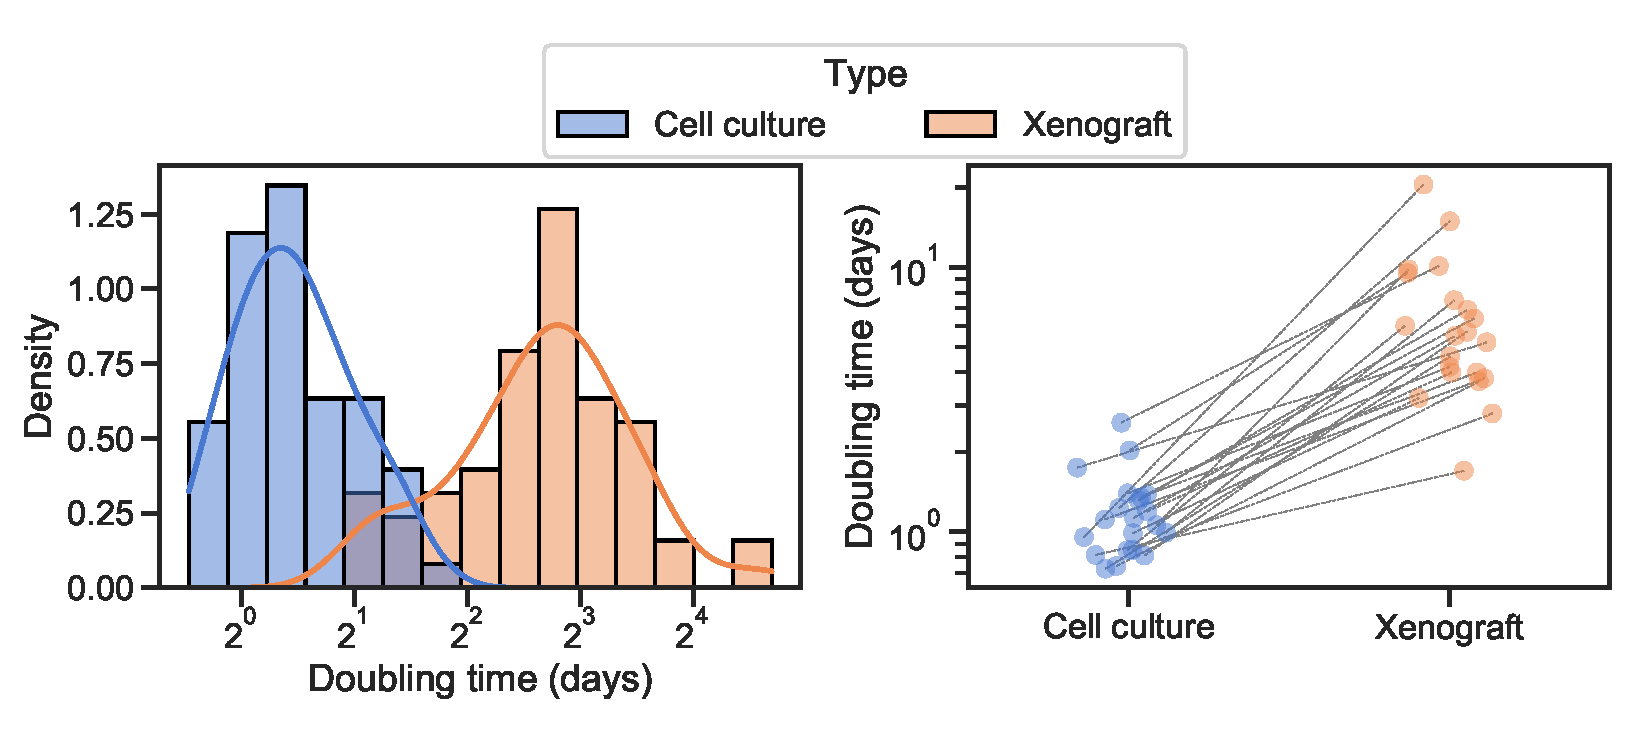
\includegraphics[width=0.70\textwidth]{figures/chap1/prlfr_contr.pdf}
    \caption[gggg]{
    gggg
    }
    \label{fig:ch1:prlfr_contr}
\end{figure}











\begin{figure}
    \centering
    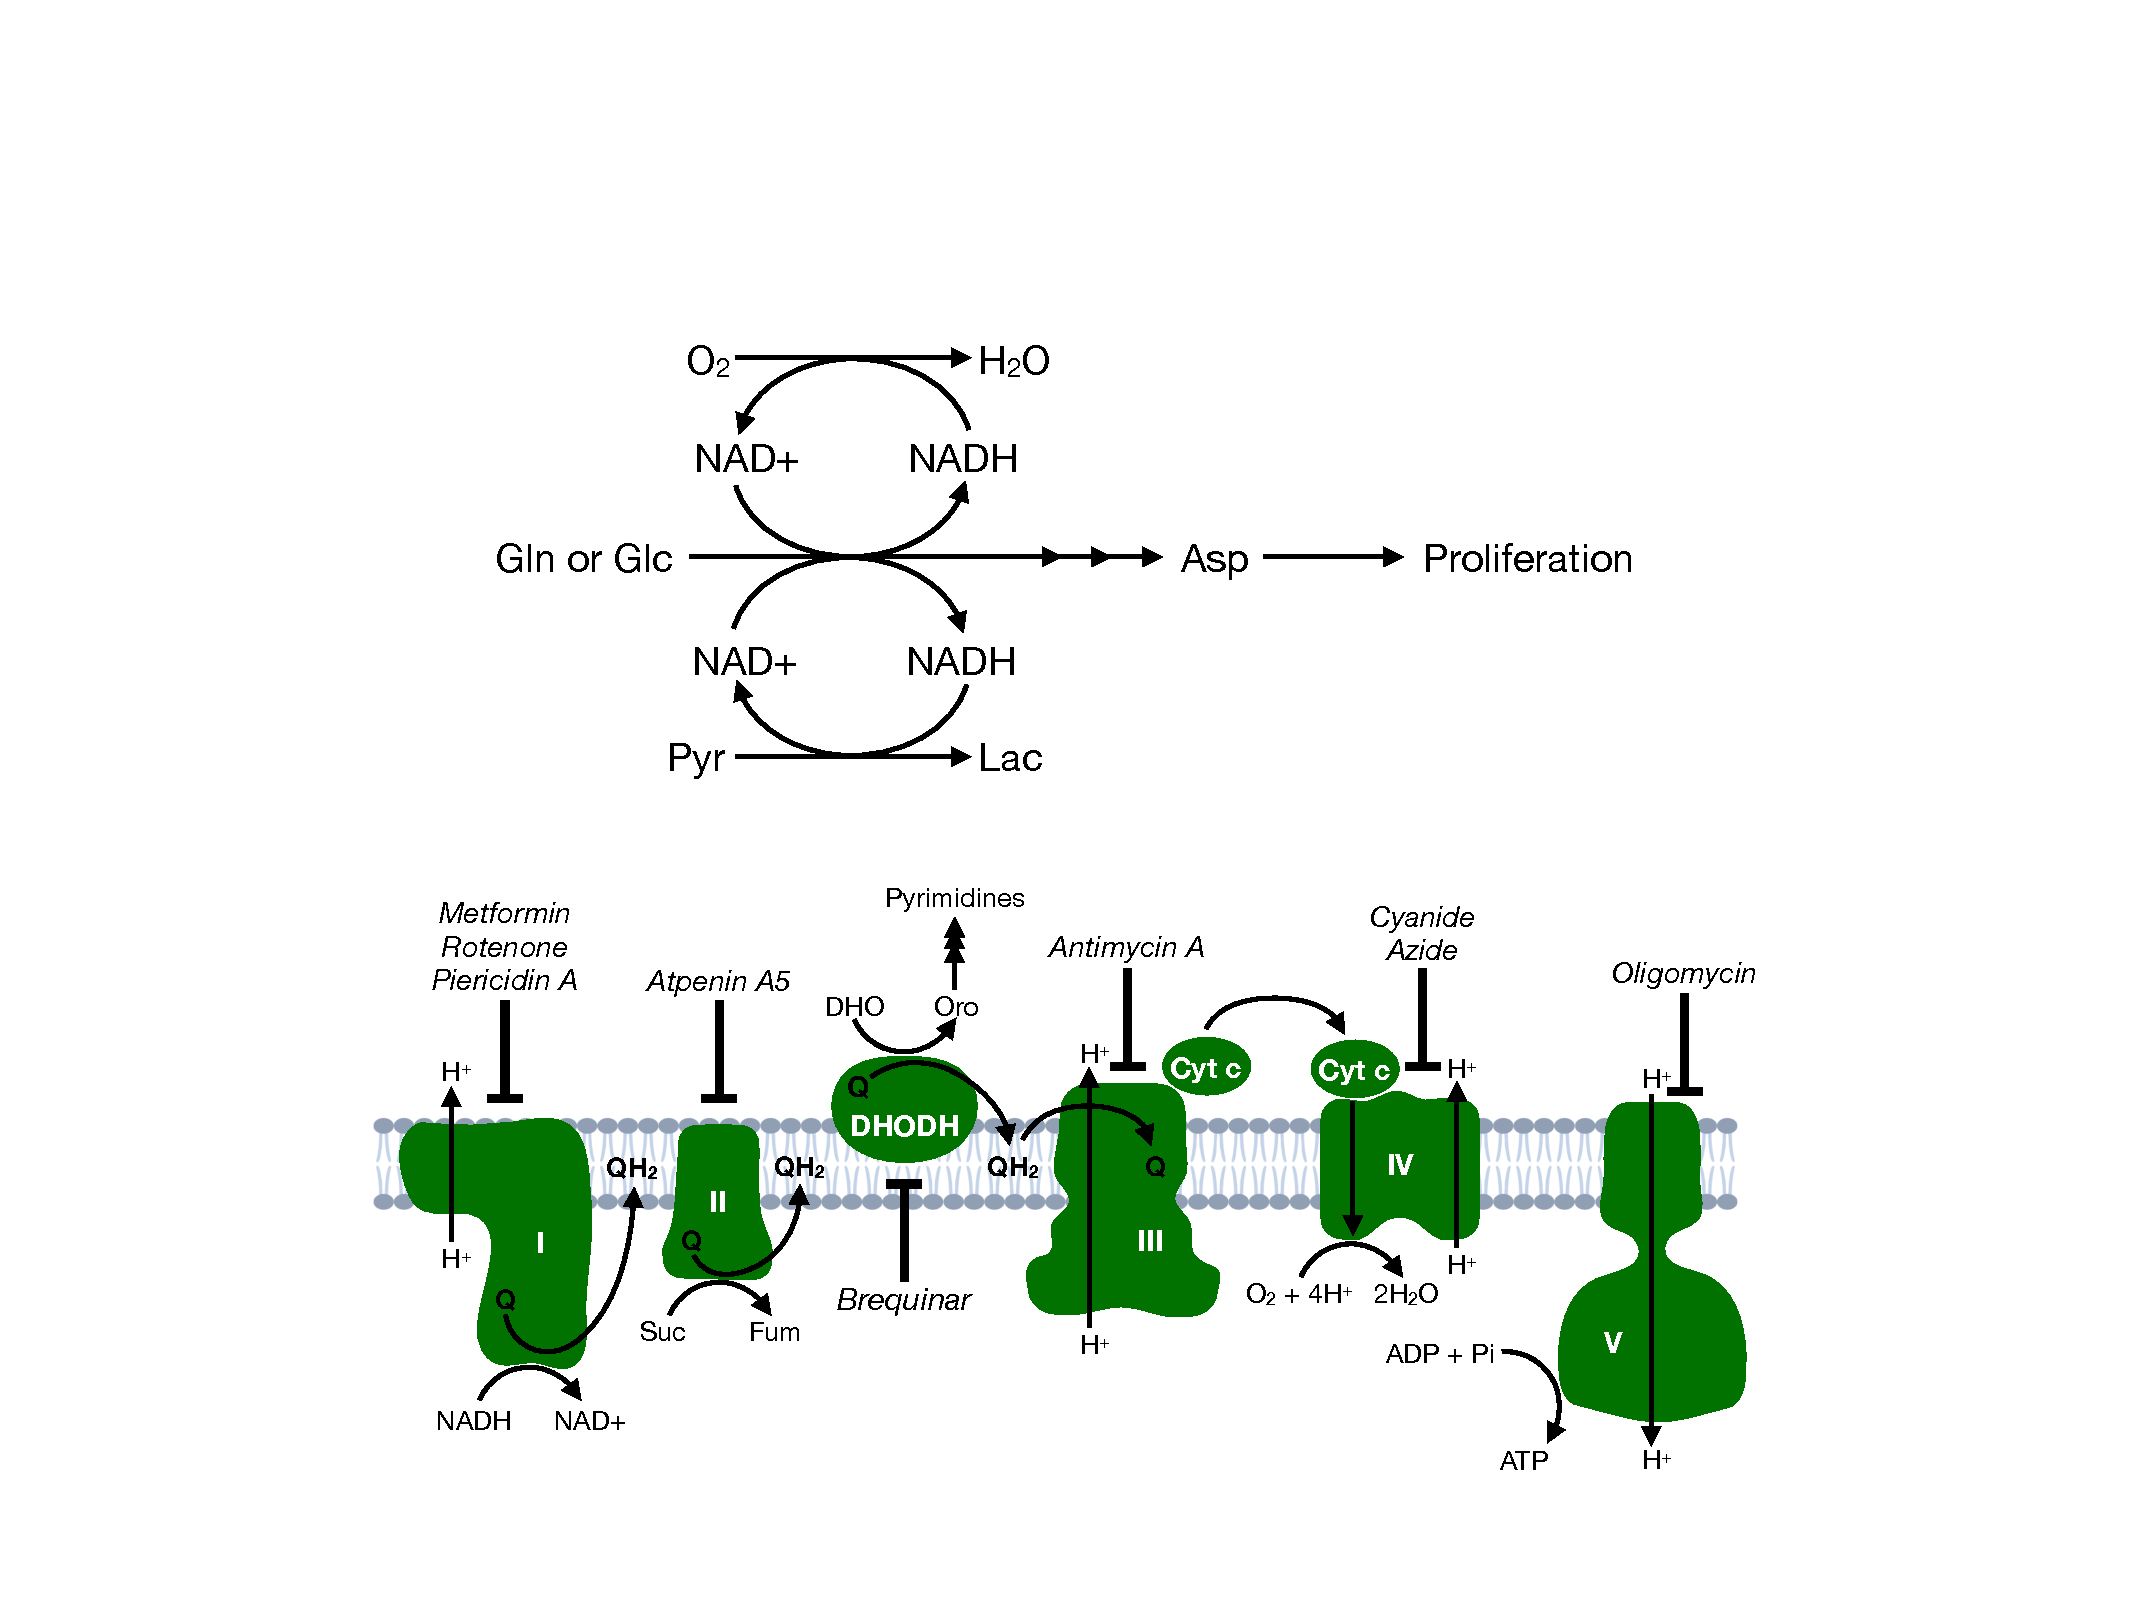
\includegraphics[width=0.70\textwidth]{figures/chap1/redox_biomass.pdf}
    \caption[Biomass accumulation requires NAD+ regeneration]{
    gggg
    }
    \label{fig:ch1:redox_biomass}
\end{figure}







Aspartate is typically coupled to NAD+/NADH ratio and thus if one is changed the other one is changed proportionally an vice versa.
Therefore it could be compelling to think that aspartate levels correlate with proliferation only indirectly through the NAD+/NADH ratio.
However, we have evidence against this:
Lucas' previous papers
My NAD+/NADH experiment with 143B SLC1A3 cells
Maddie's paper on SHDB which shows the opposite trend i.e. increased cytoplasmic NAD+/NADH ratio (due to media pyruvate) but are still aspartate limited



\begin{figure}
    \centering
    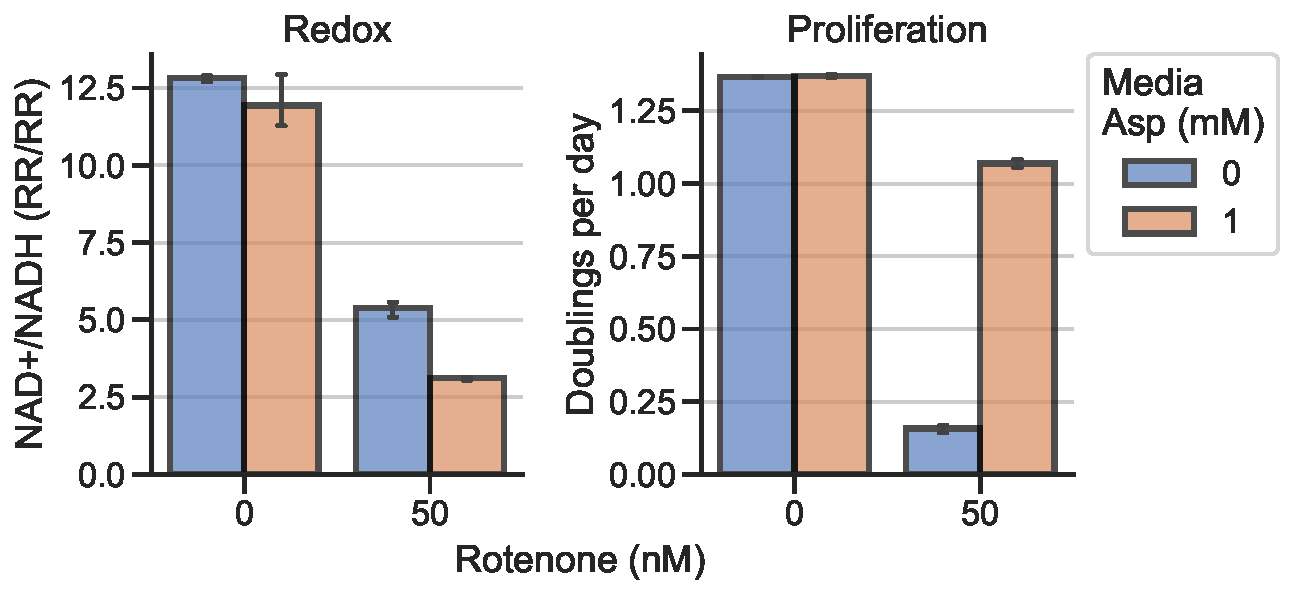
\includegraphics[width=0.70\textwidth]{figures/chap1/redox-prlfr_uncpl.pdf}
    \caption[Aspartate rescues proliferation but not the NAD+/NADH ratio]{
    Aspartate rescues proliferation but not the NAD+/NADH ratio.
    Uncoupling NAD+/NADH and aspartate's effect on proliferation using 143B cells with stable expression of the Glu/Asp transporter SLC1A3, treated with/without 1 mM media aspartate and with/without 50 nM rotenone.
    NAD+/NADH ratio measured using LCMS as a ratio between two internal standard normalized response ratios (RR/RR).
    }
    \label{fig:ch1:redox-prlfr_uncpl}
\end{figure}







\begin{figure}
    \centering
    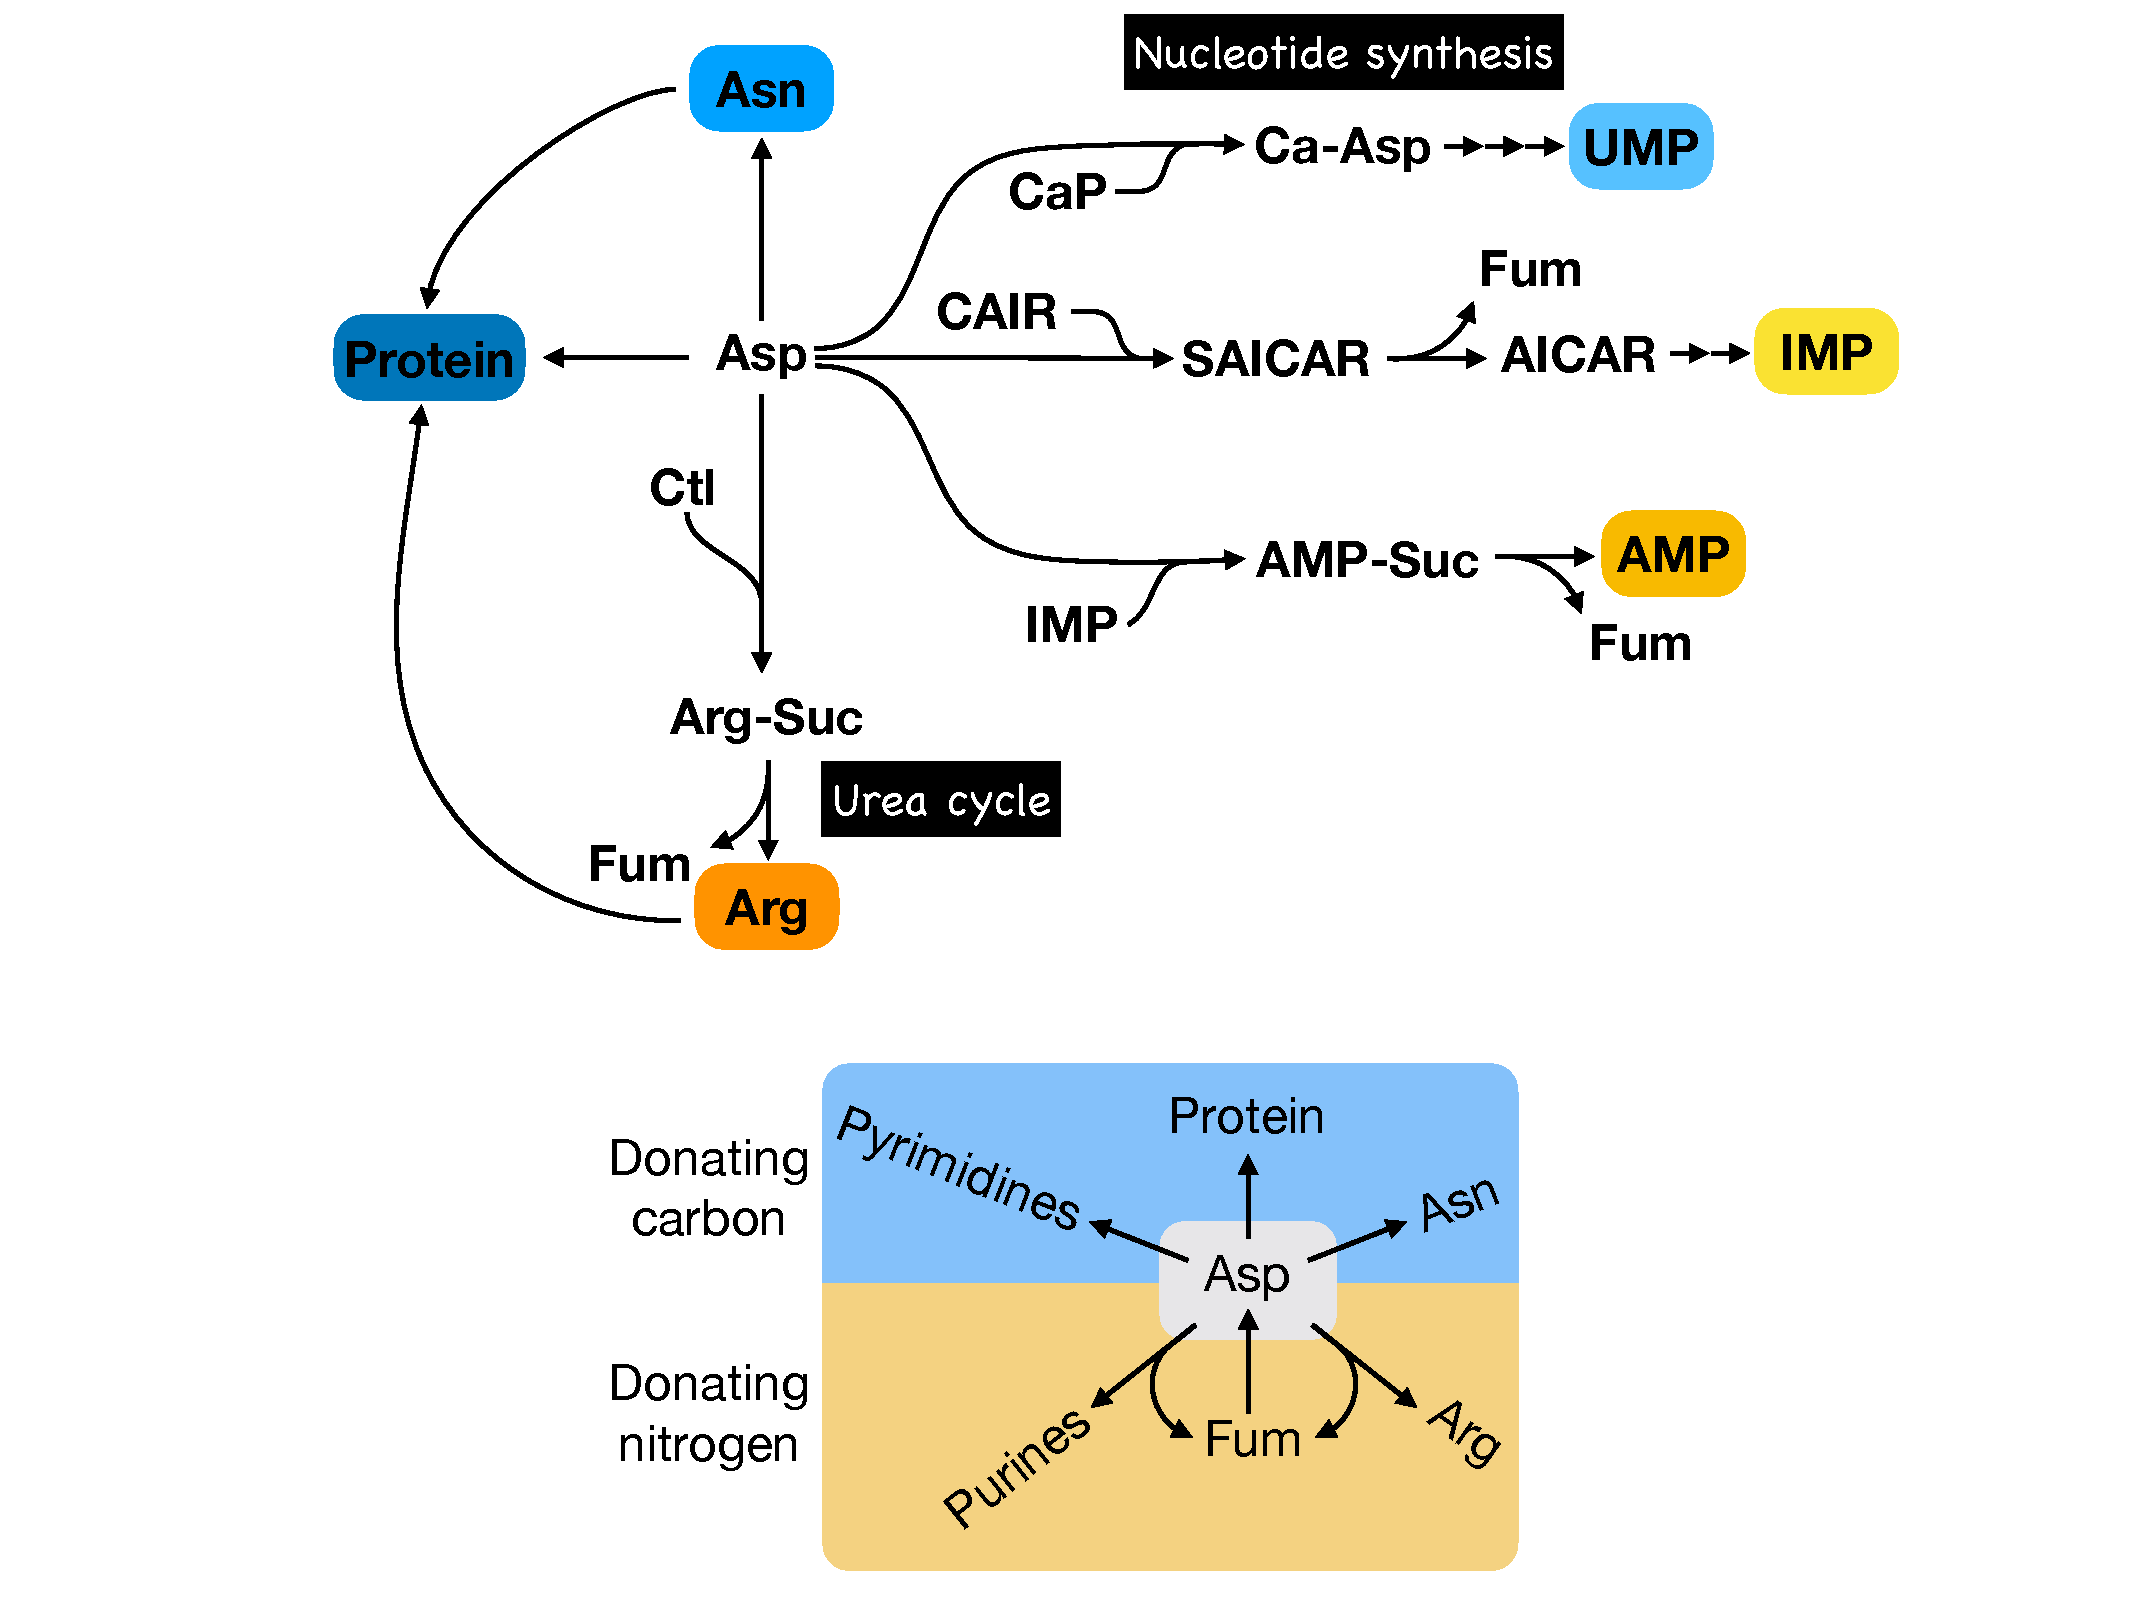
\includegraphics[width=0.70\textwidth]{figures/chap1/asp_fates.pdf}
    \caption[Metabolic fates of aspartate]{
    gggg
    }
    \label{fig:ch1:asp_fates}
\end{figure}




\begin{figure}
    \centering
    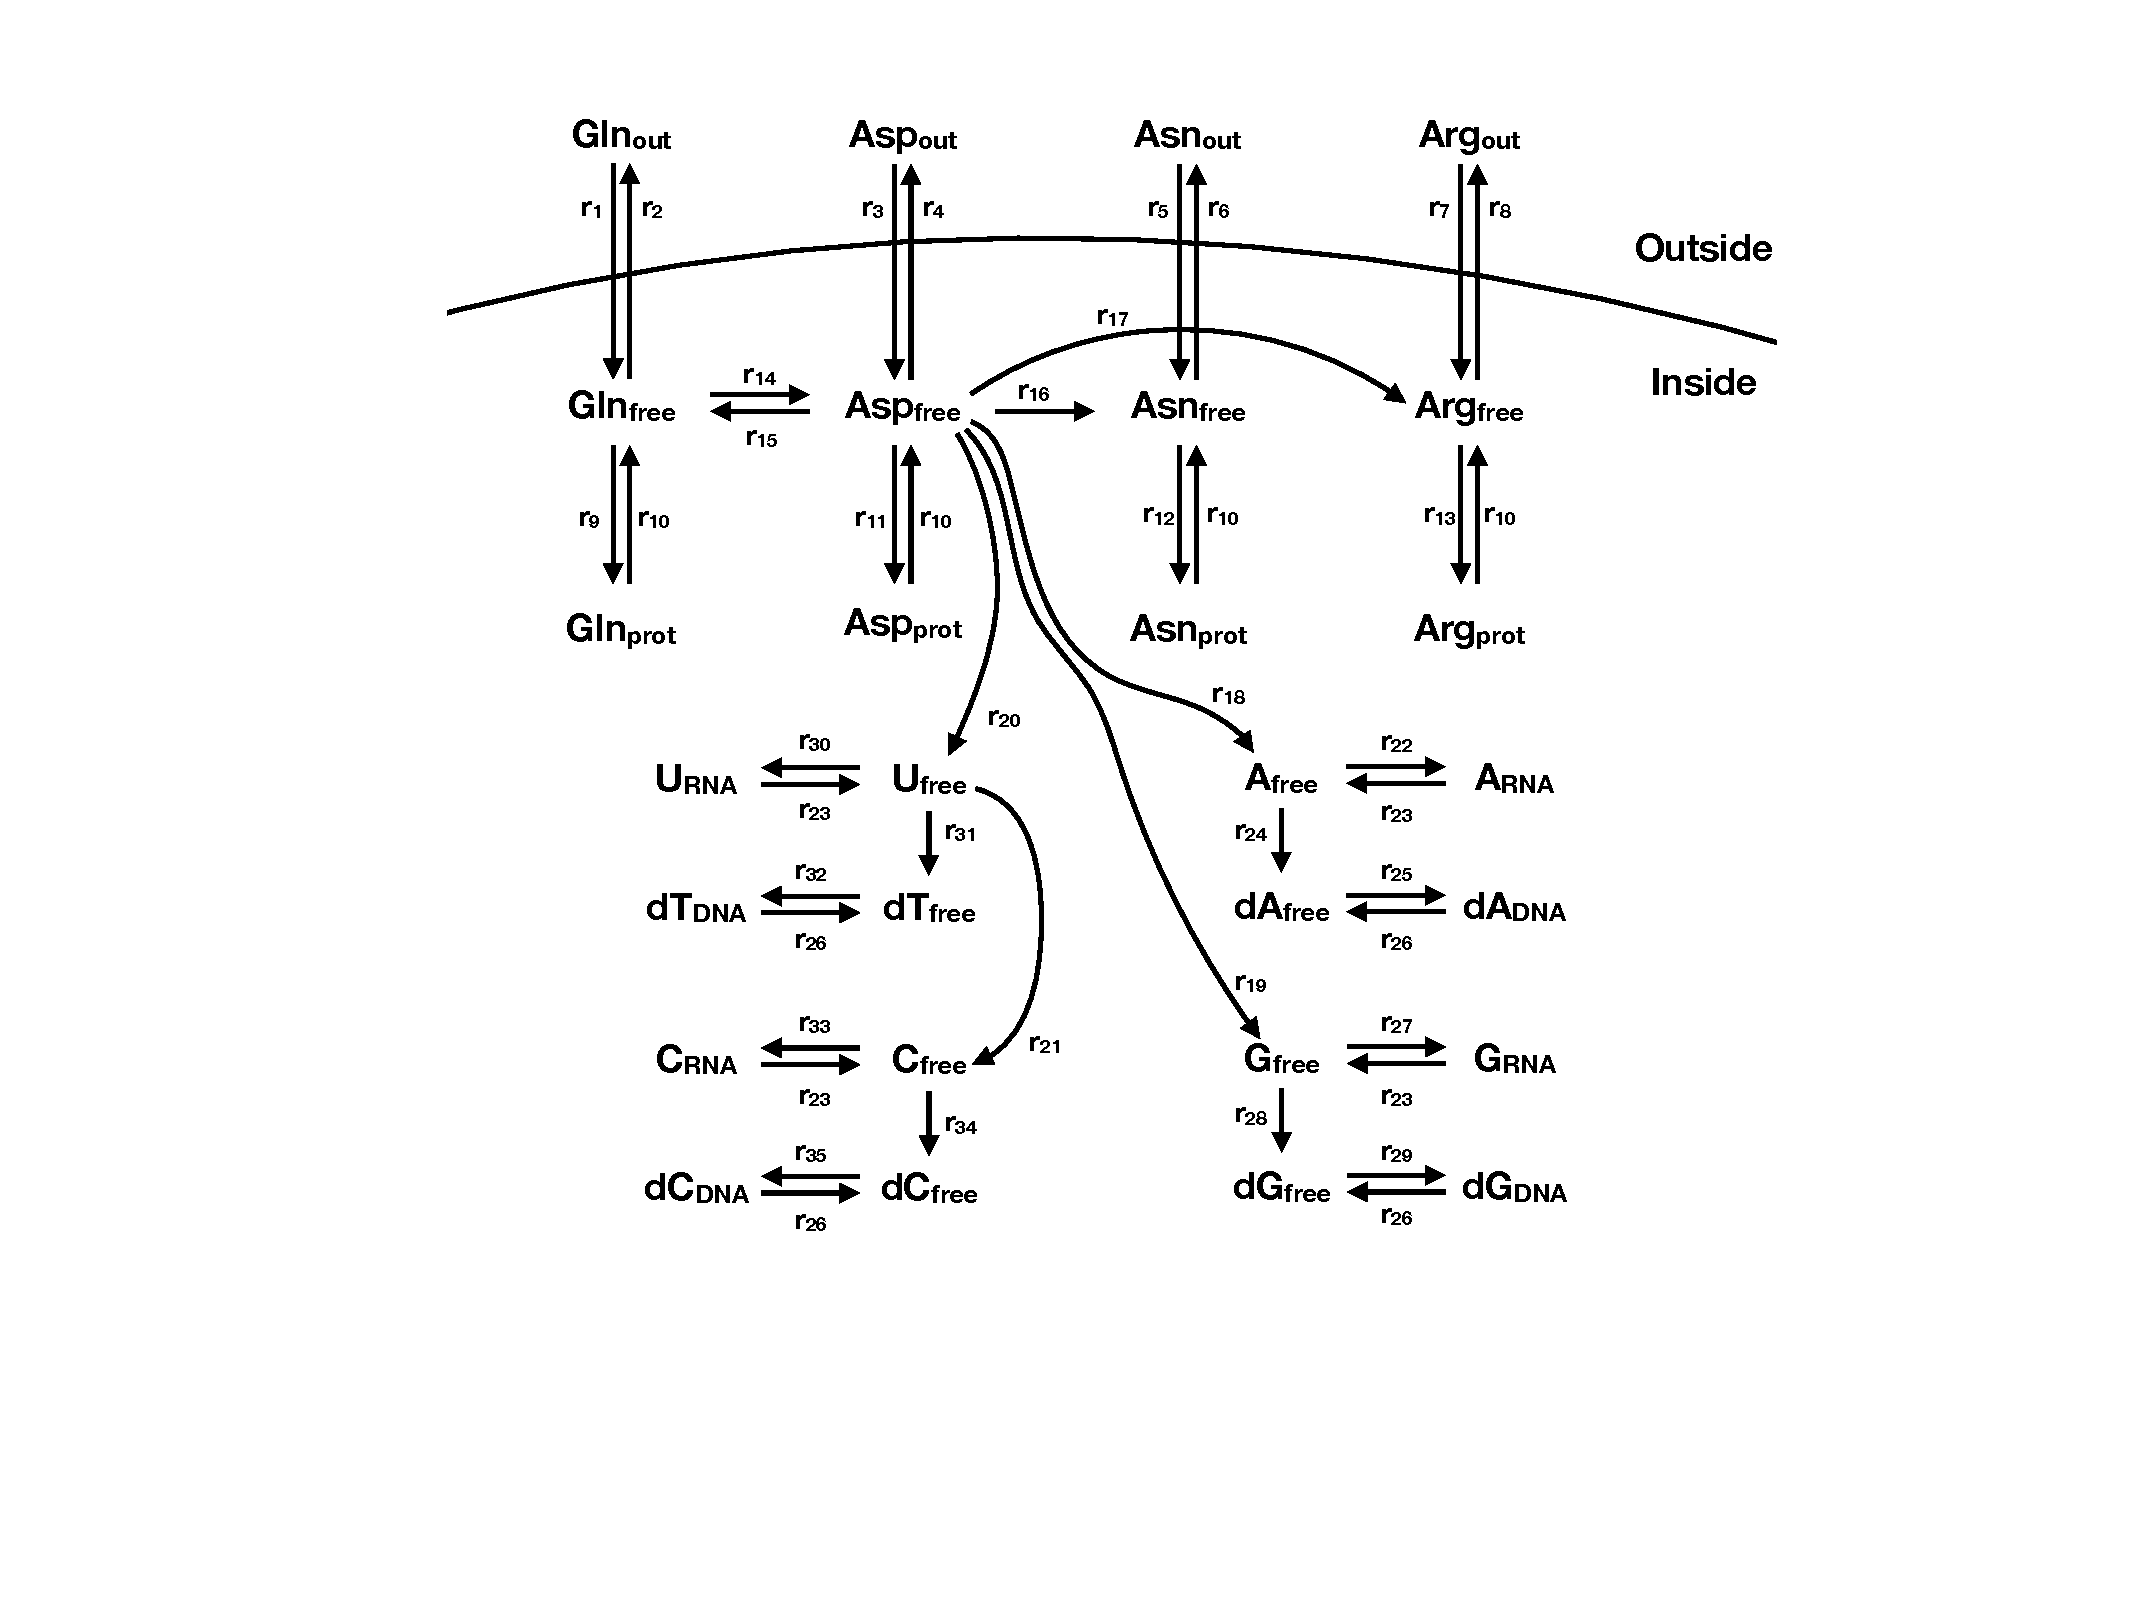
\includegraphics[width=0.70\textwidth]{figures/chap1/asp_fluxes.pdf}
    \caption[Aspartate metabolism fluxes]{
    gggg
    }
    \label{fig:ch1:asp_fluxes}
\end{figure}



\begin{figure}
    \centering
    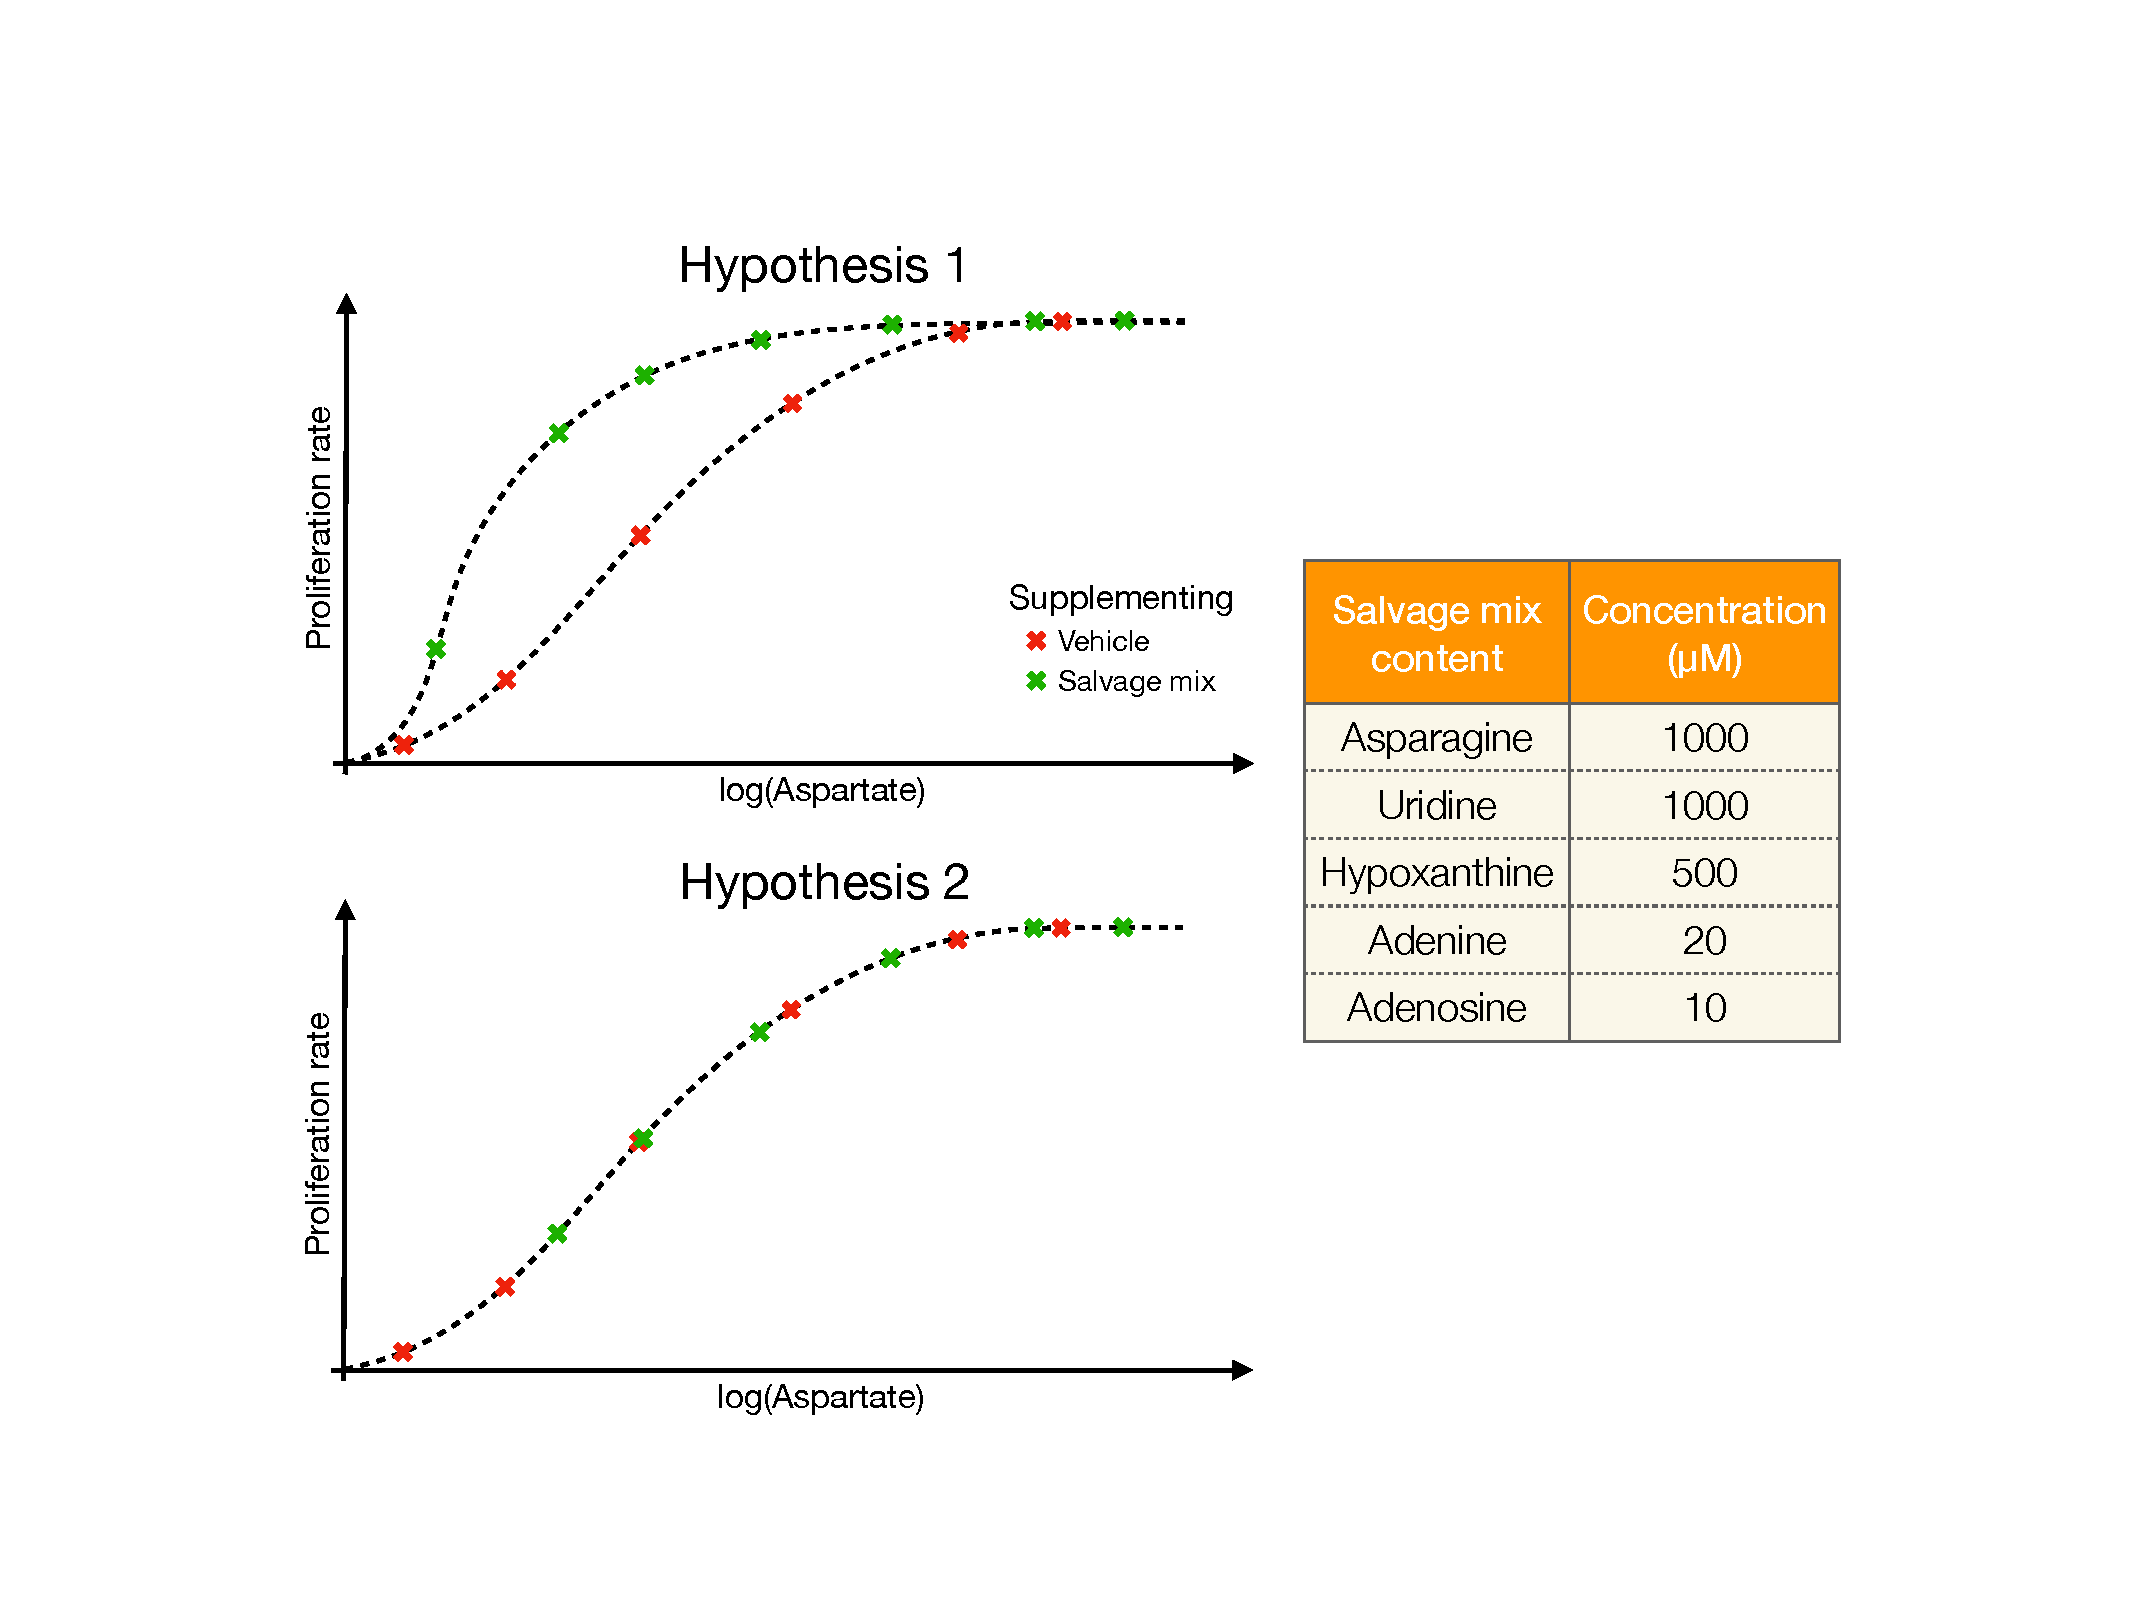
\includegraphics[width=0.70\textwidth]{figures/chap1/asp_fates_suppl_hypo.pdf}
    \caption[Two hypotheses for aspartate to proliferation correlation]{
    gggg
    }
    \label{fig:ch1:asp_fates_suppl_hypo}
\end{figure}









 % Aspartate in cellular metabolism

% All the negative data collected throughout the years:
\chapter{Molecular mechanisms of aspartate limitation}
blaa

\section{Introduction}
More blaa




\section{Mitochondrial inhibition induces a stable relationship between aspartate levels and proliferation rate}
%%% Experiments with H1299 and count/metabolites per day
%% Under ETCinhib_timeseries in lab-work







\section{Quantifying the metabolic fates of aspartate}


\begin{figure}
     \centering
     \begin{subfigure}[b]{0.75\textwidth}
         \centering
         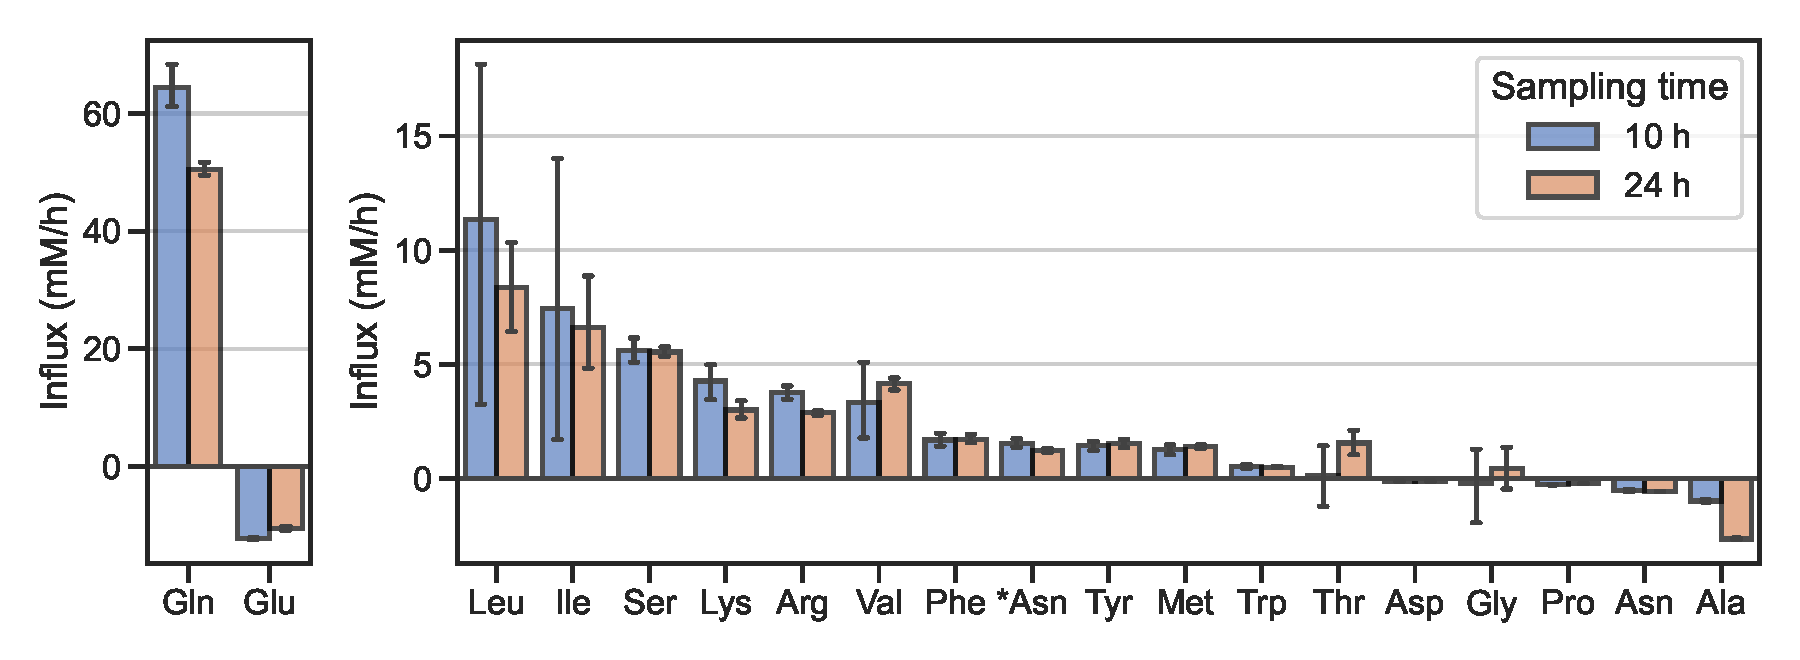
\includegraphics[width=\textwidth]{figures/chap2/flux_143wt.pdf}
         \caption{Media uptake 143B WT}
         \label{fig:ch2:flux_143wt}
     \end{subfigure}
     \begin{subfigure}[b]{0.75\textwidth}
         \centering
         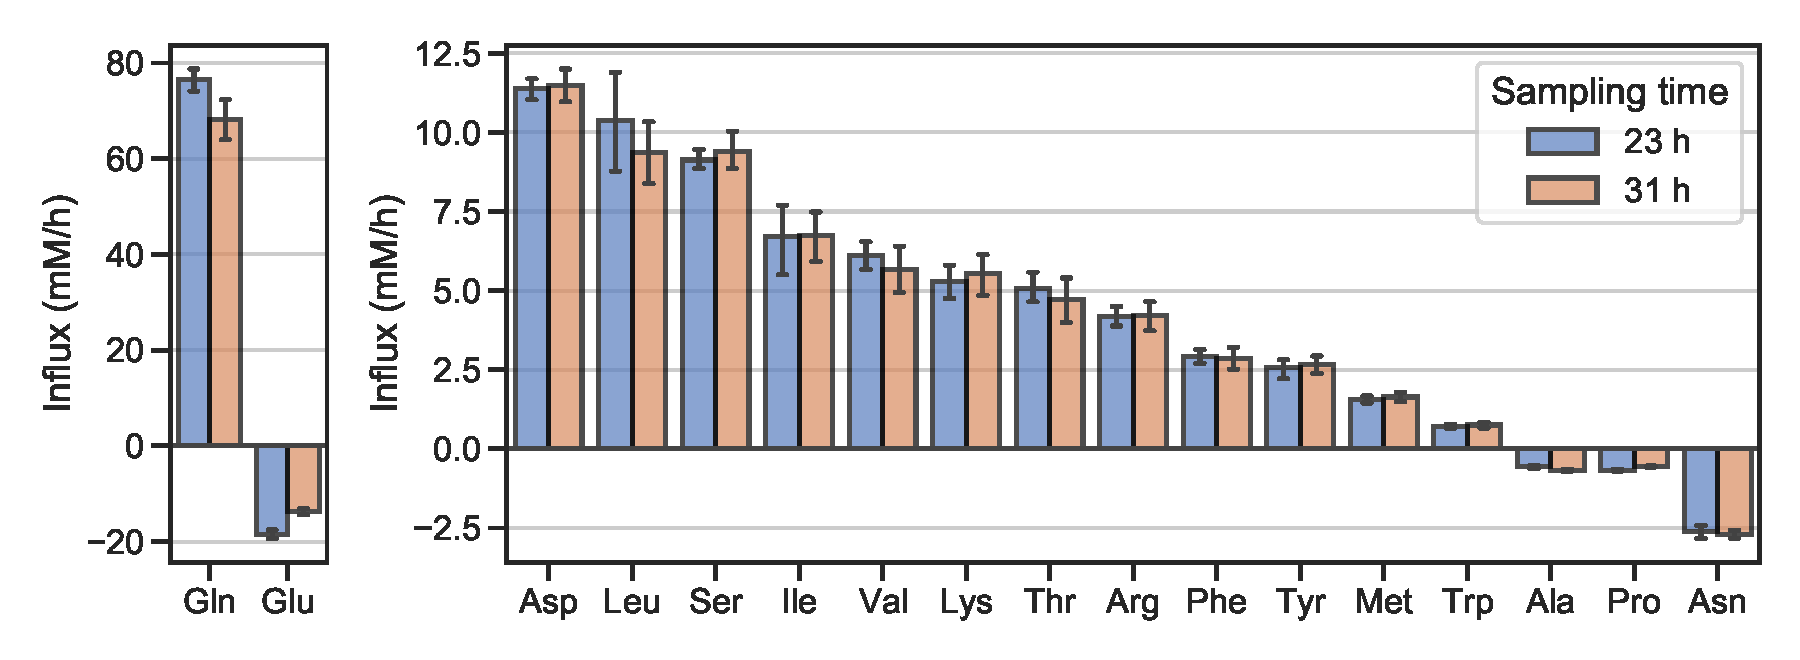
\includegraphics[width=\textwidth]{figures/chap2/flux_143dko.pdf}
         \caption{Media uptake 143B GOT DKO}
         \label{fig:ch2:flux_143dko}
     \end{subfigure}
        \caption[Media amino acid uptake]{
        Amino acid influx/efflux from DMEM.
        For 143B WT in (a), media was spiked with U-\hCi{} Asn (*Asn in the plot) to measure asparagine uptake which, taken together with the labelling fraction, was used to calculate the net asparagine consumption.
        For 143B GOT DKO in (b), cell expressed Glu/Asp transporter SLC1A3 and media was spiked with aspartate to measure its uptake.
        }
\end{figure}



Good correspondence between Asn efflux estimated through labelled Asn in 143B WT (figure \ref{fig:ch2:Asn_flux}) and measured Asn efflux in 143B GOT DKO (figure \ref{fig:ch2:flux_143dko}).
\begin{figure}
     \centering
     \hspace{0.05\textwidth}
     \begin{subfigure}[b]{0.35\textwidth}
         \centering
         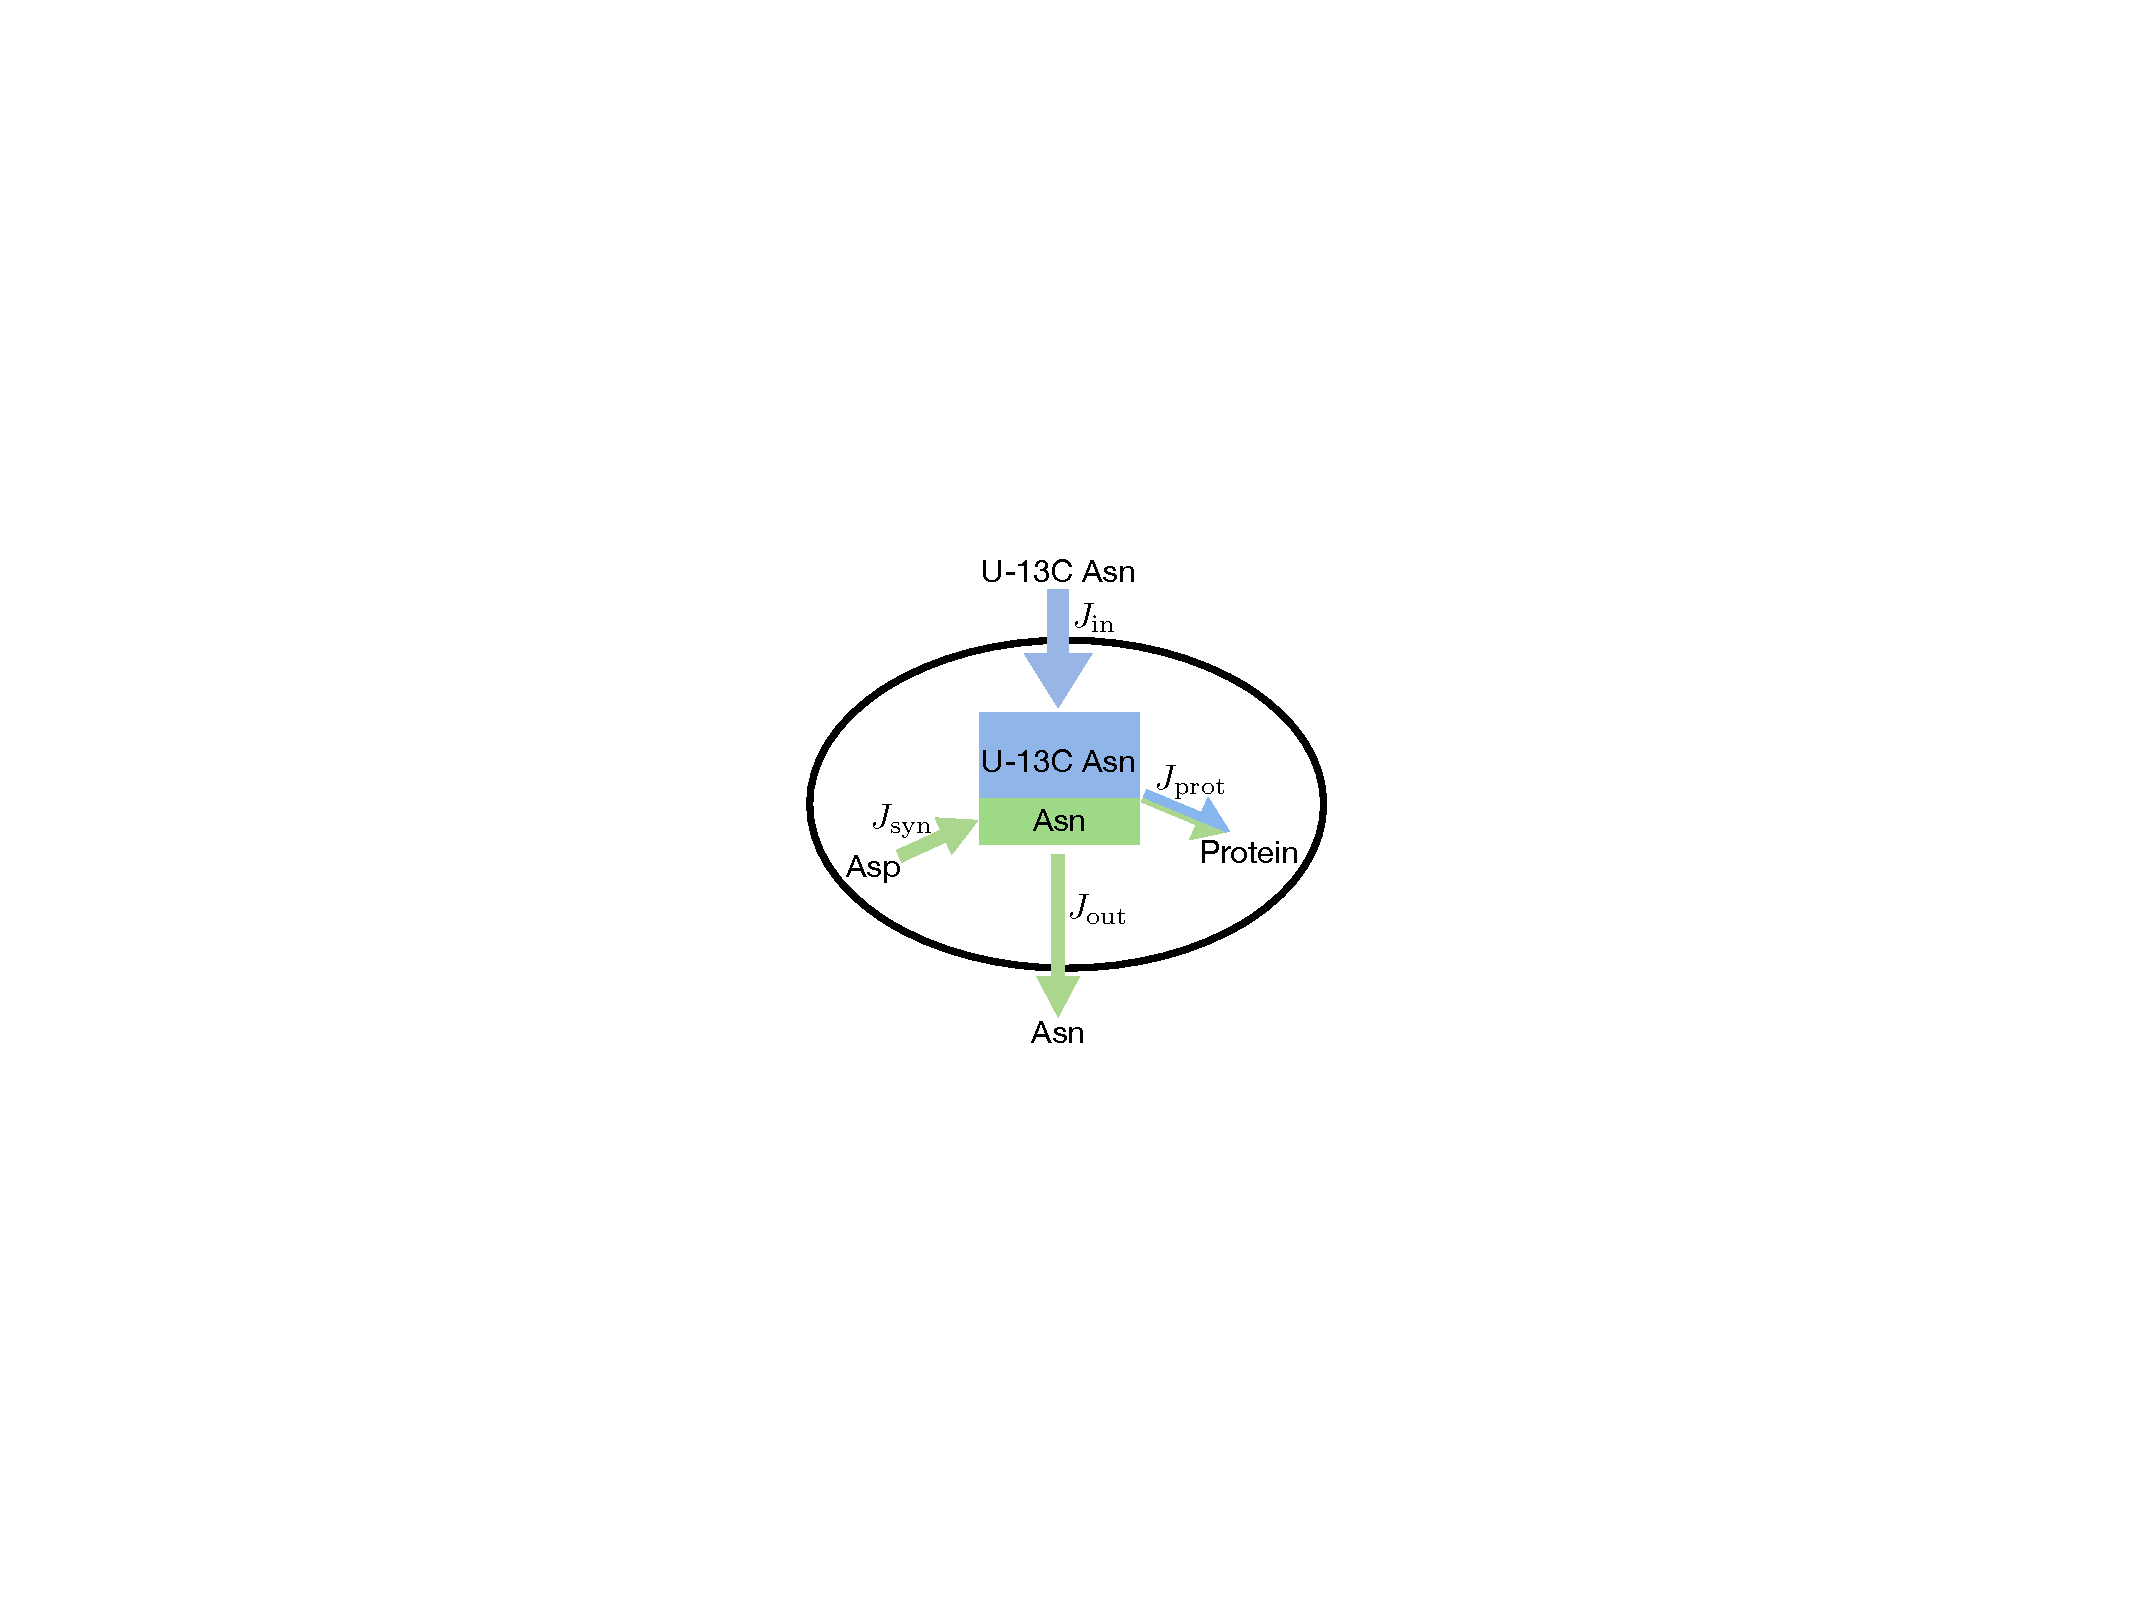
\includegraphics[width=\textwidth]{figures/chap2/asn_Jprot.pdf}
         \caption{Flux diagram}
         \label{fig:ch2:asn_Jprot}
     \end{subfigure}
     \hfill
     \begin{subfigure}[b]{0.4\textwidth}
         \centering
         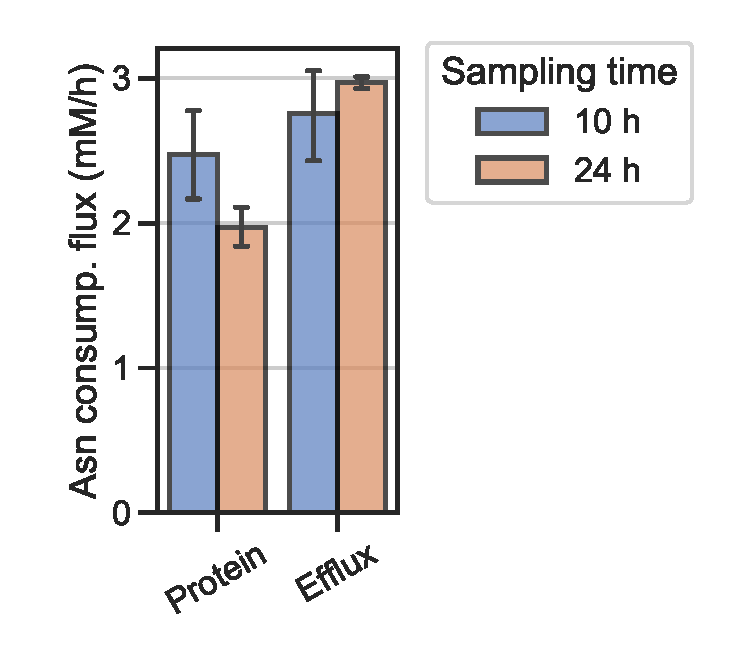
\includegraphics[width=\textwidth]{figures/chap2/Asn_flux.pdf}
         \caption{Asn consumption}
         \label{fig:ch2:Asn_flux}
     \end{subfigure}
     \hspace{0.05\textwidth}
        \caption[Asparagine consumption fluxes]{
        (a) Diagram of asparagine fluxes in a cell.
        Net influx of U-\hCi{} labelled Asn ($\Flin$), net efflux of unlabelled Asn ($\Flout$), net deposition of Asn into protein ($\Flprot$) and Asn synthesis from Asp ($\Flsyn$).
        Asn symbolized by green and U-\hCi{} Asn symbolized by blue.
        (b) Measured asparagine consumption fluxes in 143B cells using the media uptake data from figure \ref{fig:ch2:flux_143wt}.
        Asn is consumed into protein synthesis (Protein) and leaked into the media (Efflux).
        Efflux is calculated assuming no Asn is provided in the media.
        }
\end{figure}



Most of cellular biomass is amino acids \cite{Hosios2016-us}

\begin{figure}
    \centering
    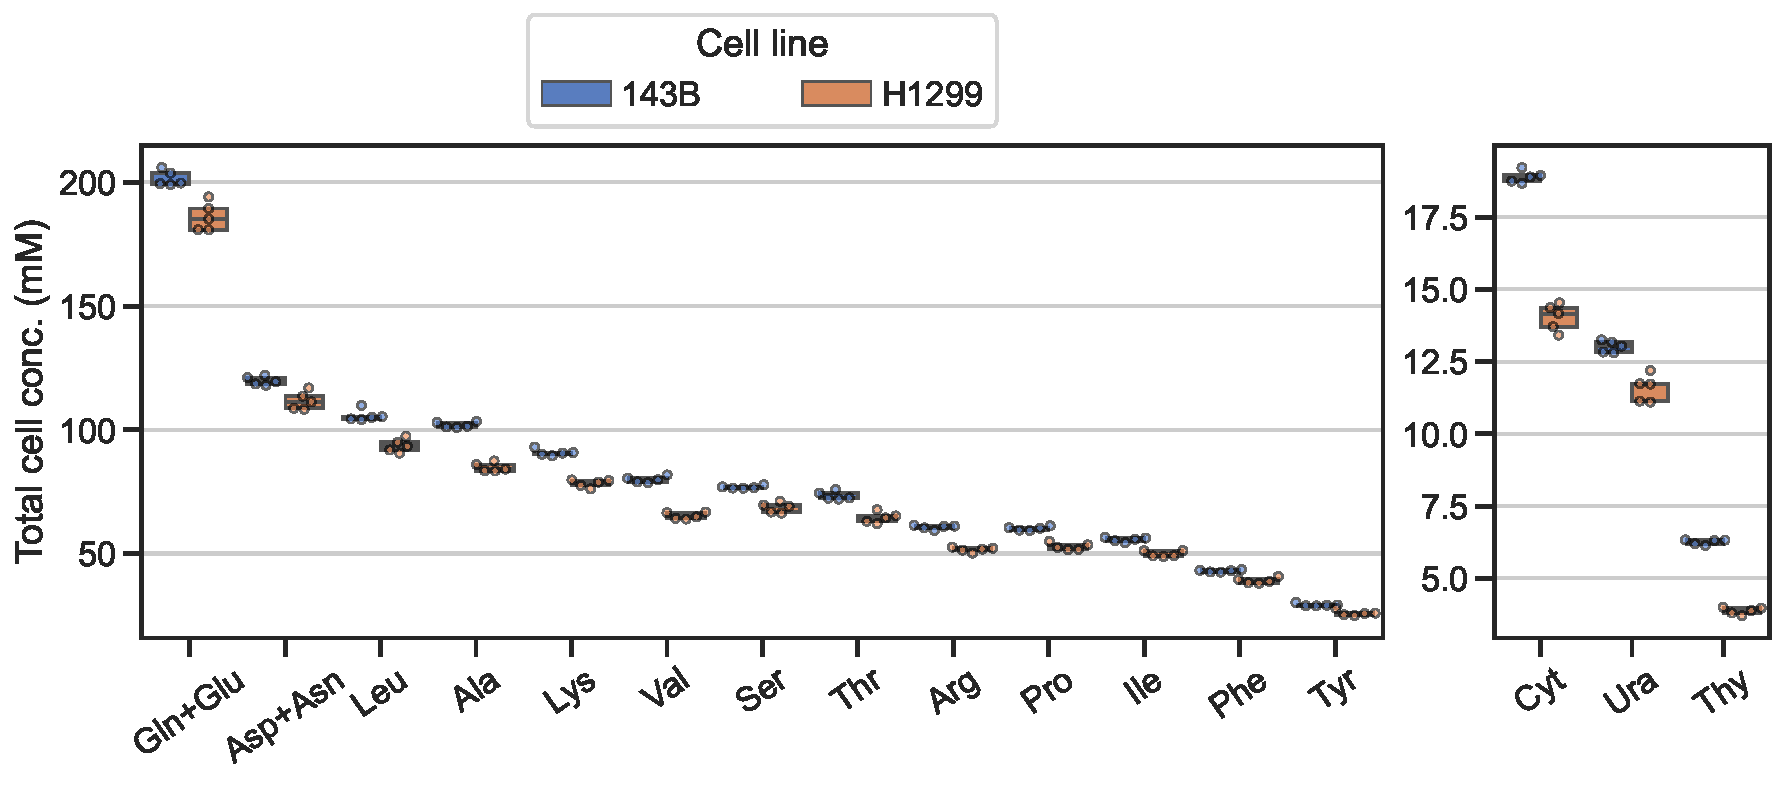
\includegraphics[width=0.80\textwidth]{figures/chap2/ah_cell_comp.pdf}
    \caption[Amino acid and pyrimidine total cell concentration]{
    Total amino acids and pyrimidines liberated by acid hydrolysis of 143B and H1299 cells, normalized by total cell volume (Total cell conc.).
    Gln and Asn is converted during acid hydrolysis to Glu and Asp respectively.
    }
    \label{fig:ch2:ah_cell_comp}
\end{figure}






The total Asp consumption flux expected in DMEM i.e. with Arg but without Asn, is estimated to be 9.25 mM/h.
This is close to Asp uptake in 143B GOT DKO which was measured at 11.43 mM/h (figure \ref{fig:ch2:flux_143dko}).
The difference is directionally as would be expected because total pyrimidine/purine levels underestimate synthesis flux by discounting recycling (figure ]\ref{fig:ch2:pur_tr_ov}) and because 143B GOT DKO maintain a higher intracellular concentration of aspartate due to expression of Glu/Asp transporter SLC1A3.
\begin{figure}
    \centering
    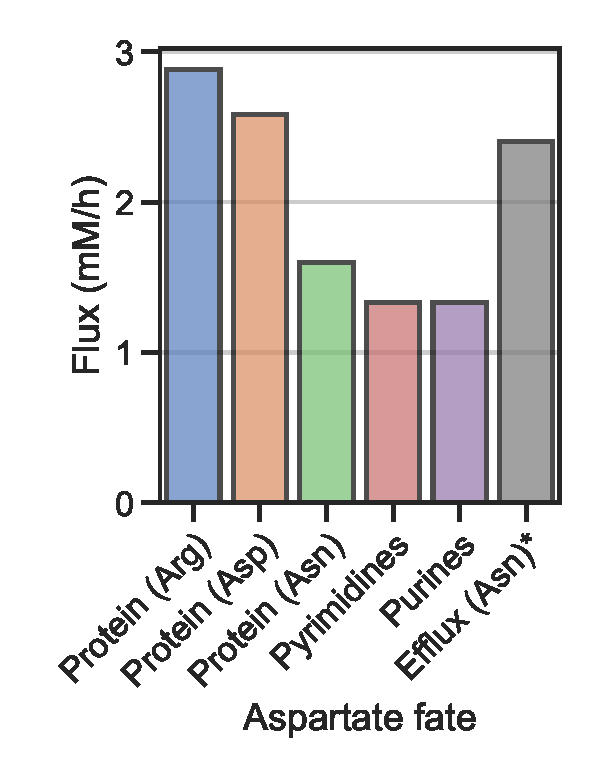
\includegraphics[width=0.36\textwidth]{figures/chap2/asp_fate.pdf}
    \caption[Relative consumption towards each fate of aspartate]{
    Relative consumption towards each fate of aspartate estimated using best estimates from figure \ref{fig:ch2:Asn_flux} and \ref{fig:ch2:ah_cell_comp}.
    Aspartate consumption towards purines was estimated equal to consumption towards pyrimidines.
    * Asn efflux is calculated based on the assumption that cells are grown in asparagine free media, prior to substantial media conditioning.
    }
    \label{fig:ch2:asp_fate}
\end{figure}






\section{Salvage of the metabolic fates of aspartate}

\subsection{Salvage mix fulfills all the metabolic fates of aspartate}

metabolic fates of aspartate i.e. aspartate conversion 


\begin{figure}
    \centering
    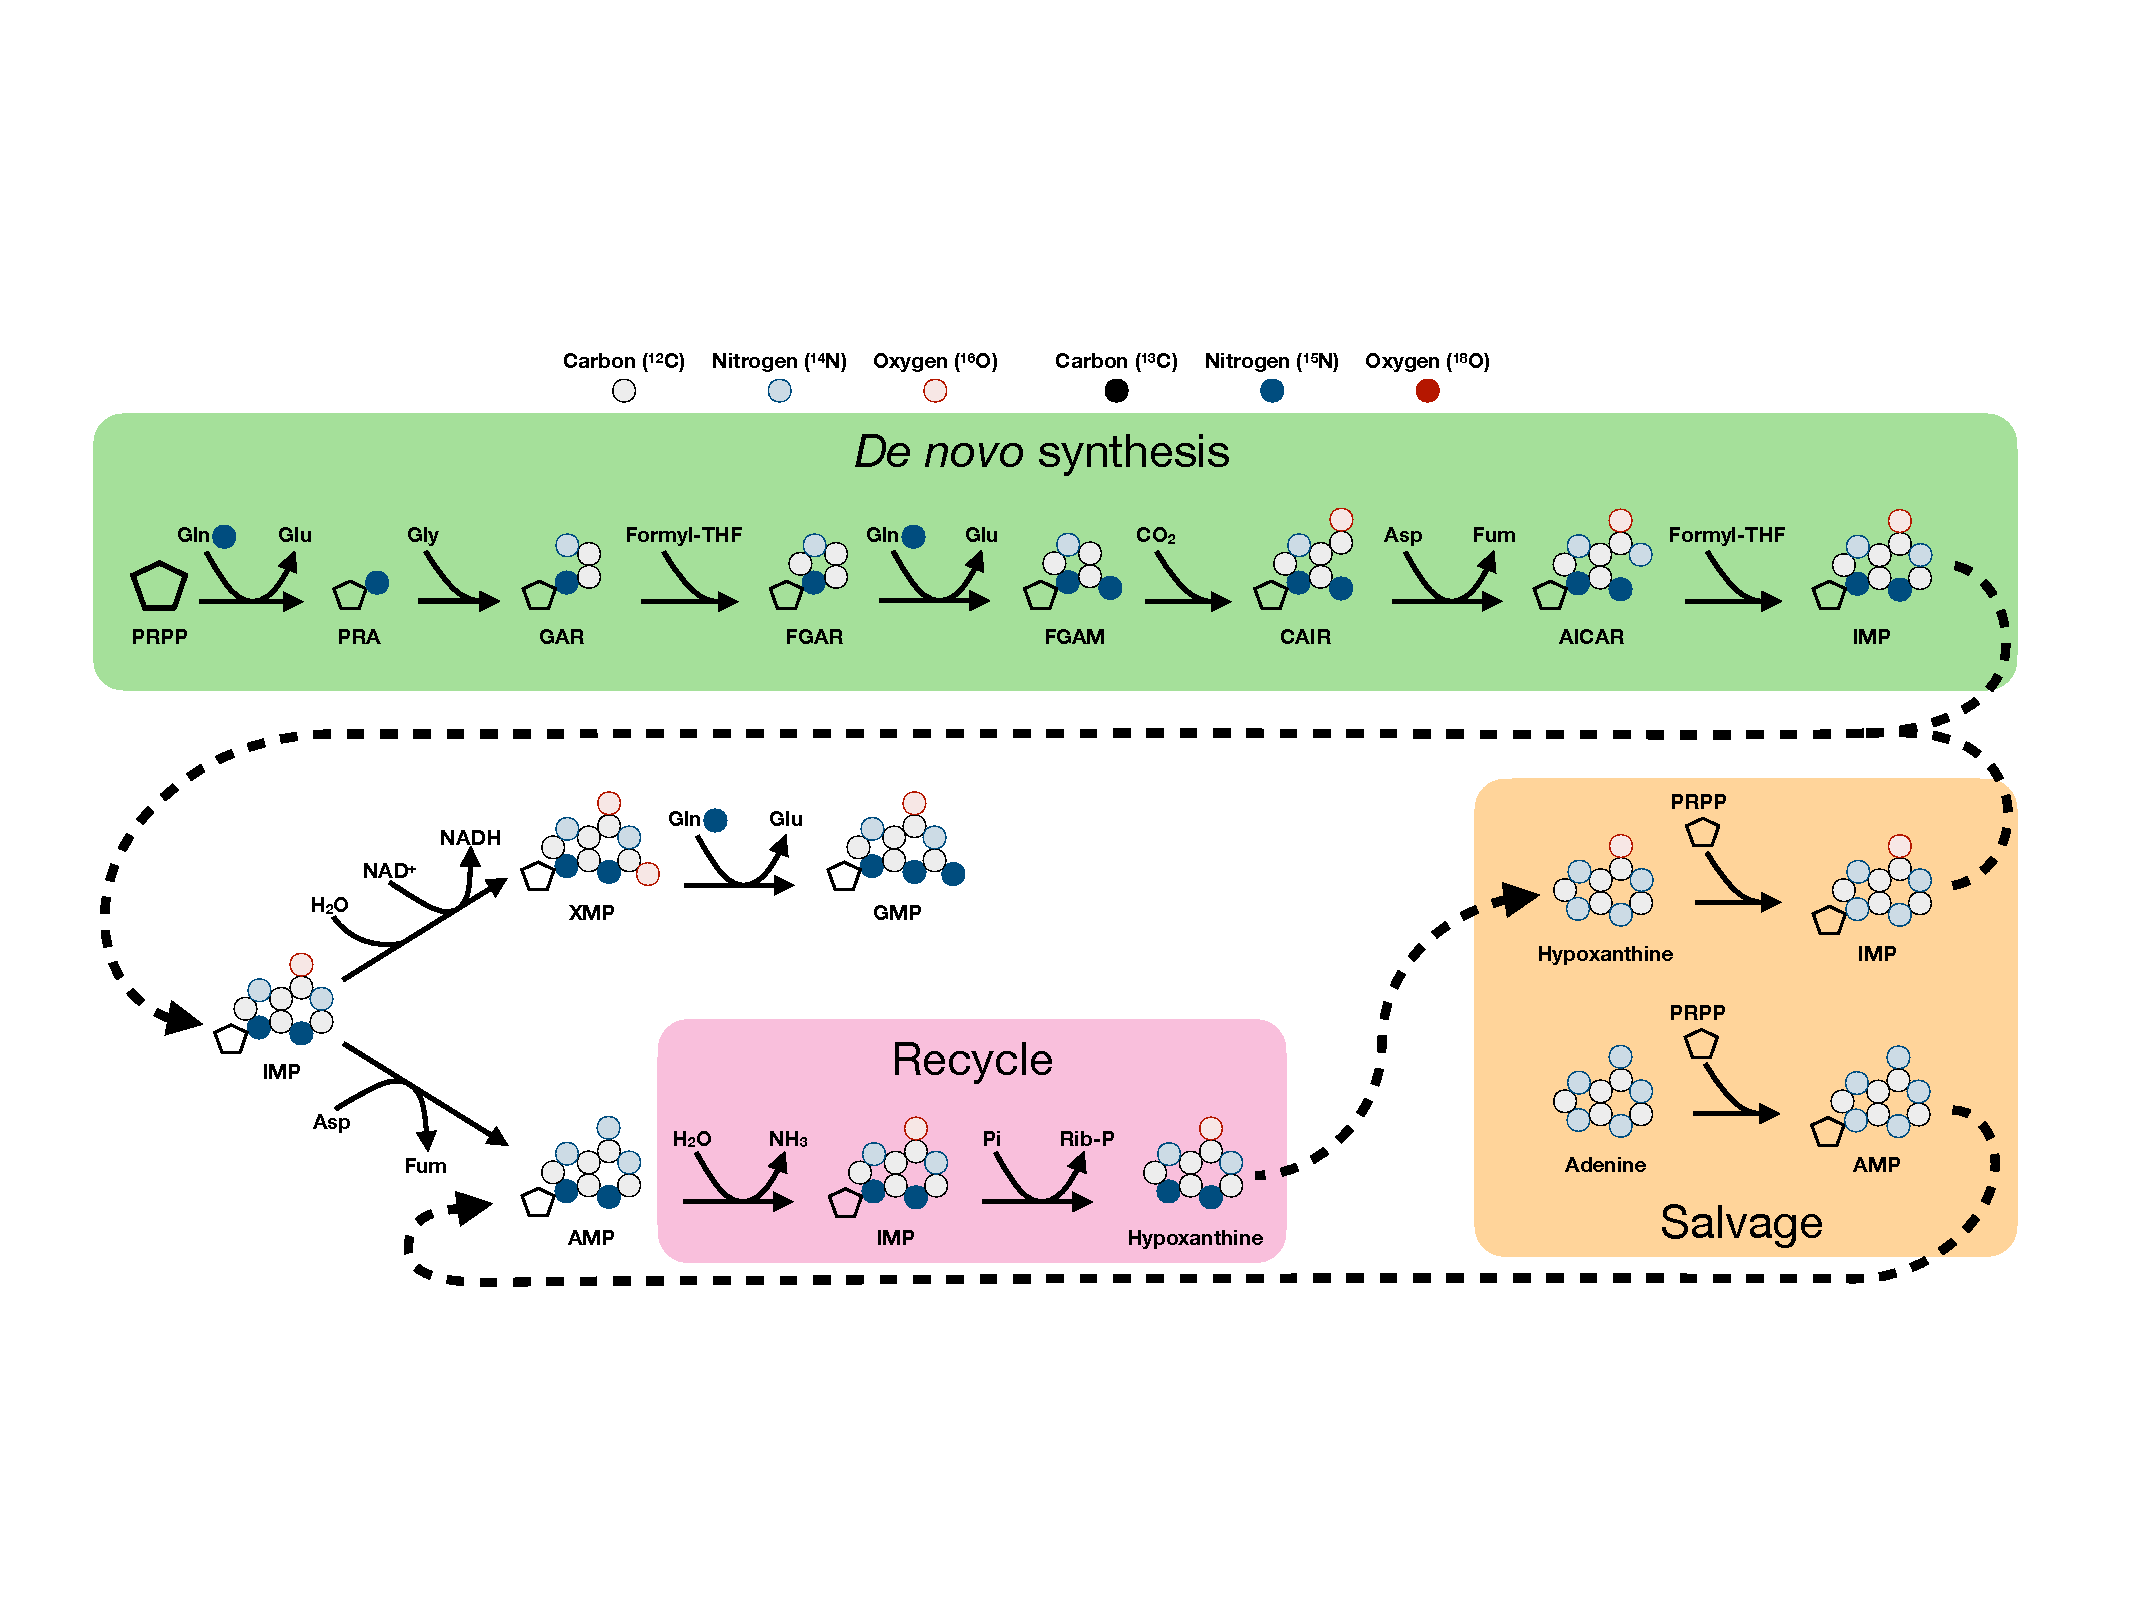
\includegraphics[width=0.95\textwidth]{figures/chap2/purine_tracing_overvew.pdf}
    \caption[Purine metabolism \hNi-amide Gln tracing overview]{
    Overview of \hNi-amide Gln label incorporation in \textit{de novo} purine synthesis.
    Label incorporation can be effected by salvage of unlabelled hypoxanthine or adenine and recycling as it appears on the overview.
    }
    \label{fig:ch2:pur_tr_ov}
\end{figure}





\begin{figure}
    \centering
    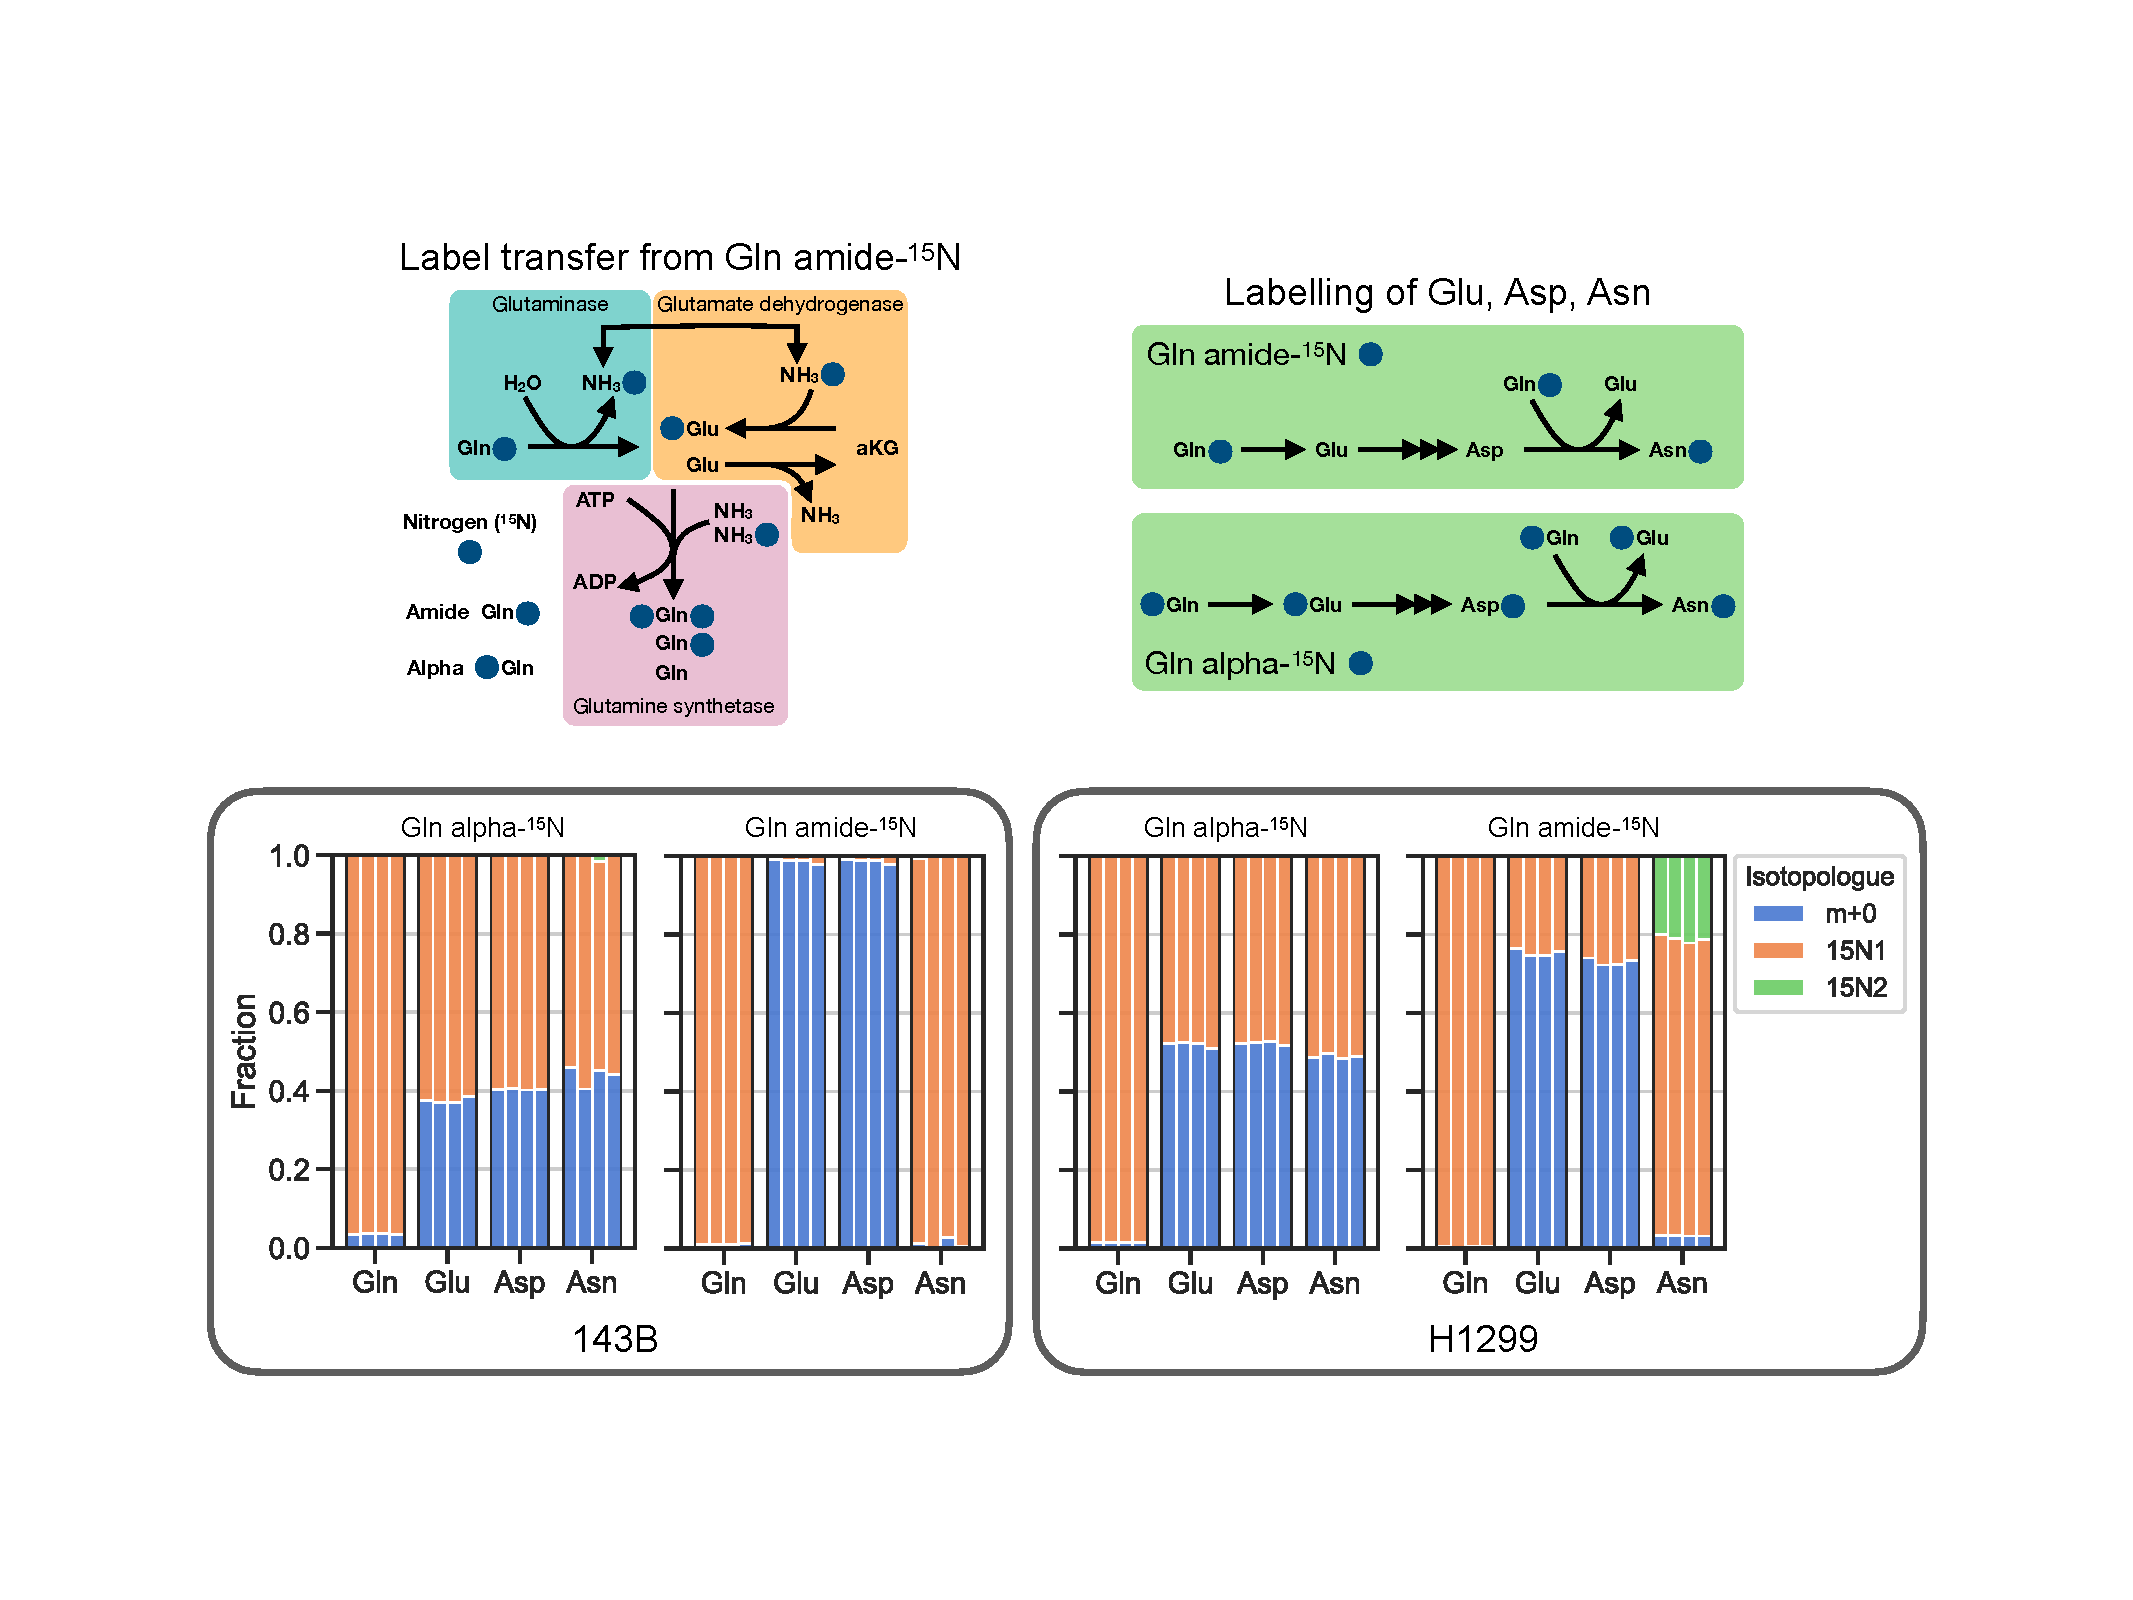
\includegraphics[width=0.95\textwidth]{figures/chap2/gln_lab_tranfr.pdf}
    \caption[Gln amide to alpha \hNi{} transfer]{
    Gln \hNi{} on the amide nitrogen can transfer to the alpha nitrogen in H1299 cells but not in 143B cells.
    Upper left diagram shows how Gln amide and alpha nitrogen labels can transfer.
    Transfer of amide labelled nitrogen can be achieved by glutaminase catalyzed release of labelled ammonia and its subsequent use as a substrate in the conversion of alpha-ketoglutarate (aKG) to Glu alpha-\hNi by glutamate dehydrogenase.
    The signature of glutamine synthetase activity is the appearance of doubly labelled Gln.
    Upper right diagram shows how Gln amide and alpha nitrogen labels are transferred to downstream metabolites Glu, Asp and Asn.
    Lower panel shows the nitrogen isotopologue distribution of Gln, Glu, Asp and Asn in 143B and H1299 at steady-state.
    The alpha nitrogen label is frequently lost in Glu and downstream, presumably due to transaminase catalyzed exchange with unlabelled amino groups on amino acids such as leucine, isoleucine, valine etc.
    The amide nitrogen label is partially transferred to the alpha position in H1299, but not in 143B, also indicated by the doubly labelled Asn.
    }
    \label{fig:ch2:gln_lab_tranfr}
\end{figure}


\begin{figure}
    \centering
    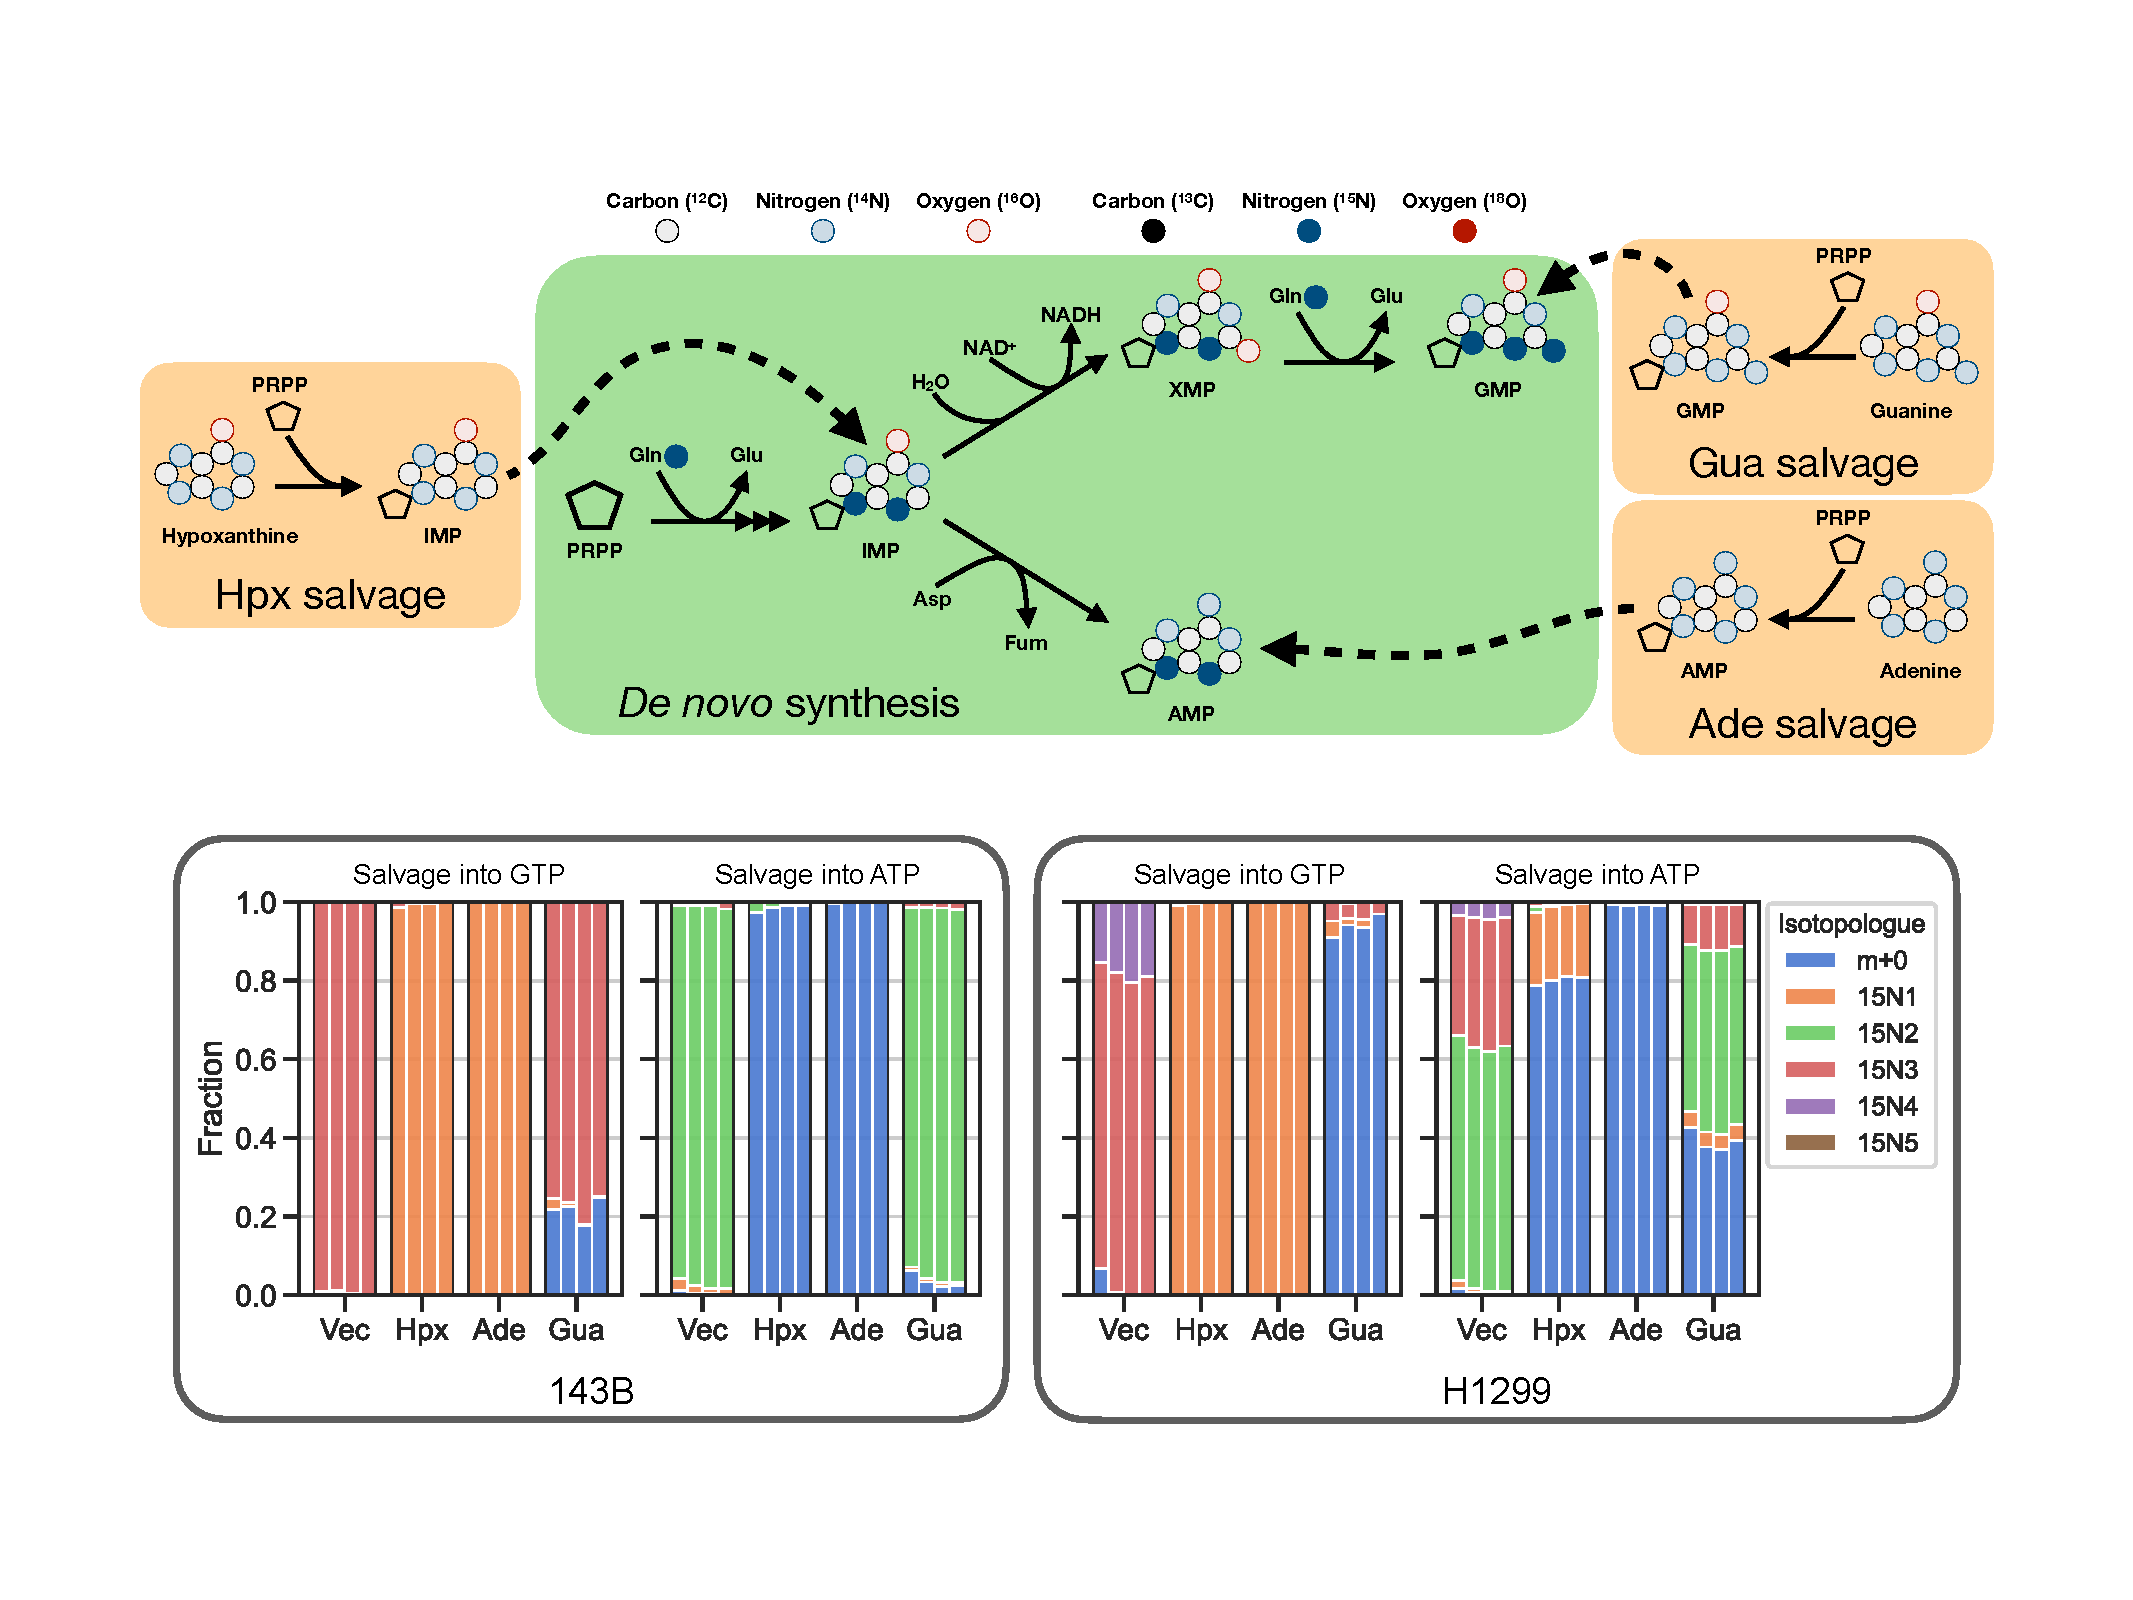
\includegraphics[width=0.98\textwidth]{figures/chap2/sal_frac_pur.pdf}
    \caption[Salvage into purines]{
    ggg
    }
    \label{fig:ch2:sal_frac_pur}
\end{figure}


\begin{figure}
    \centering
    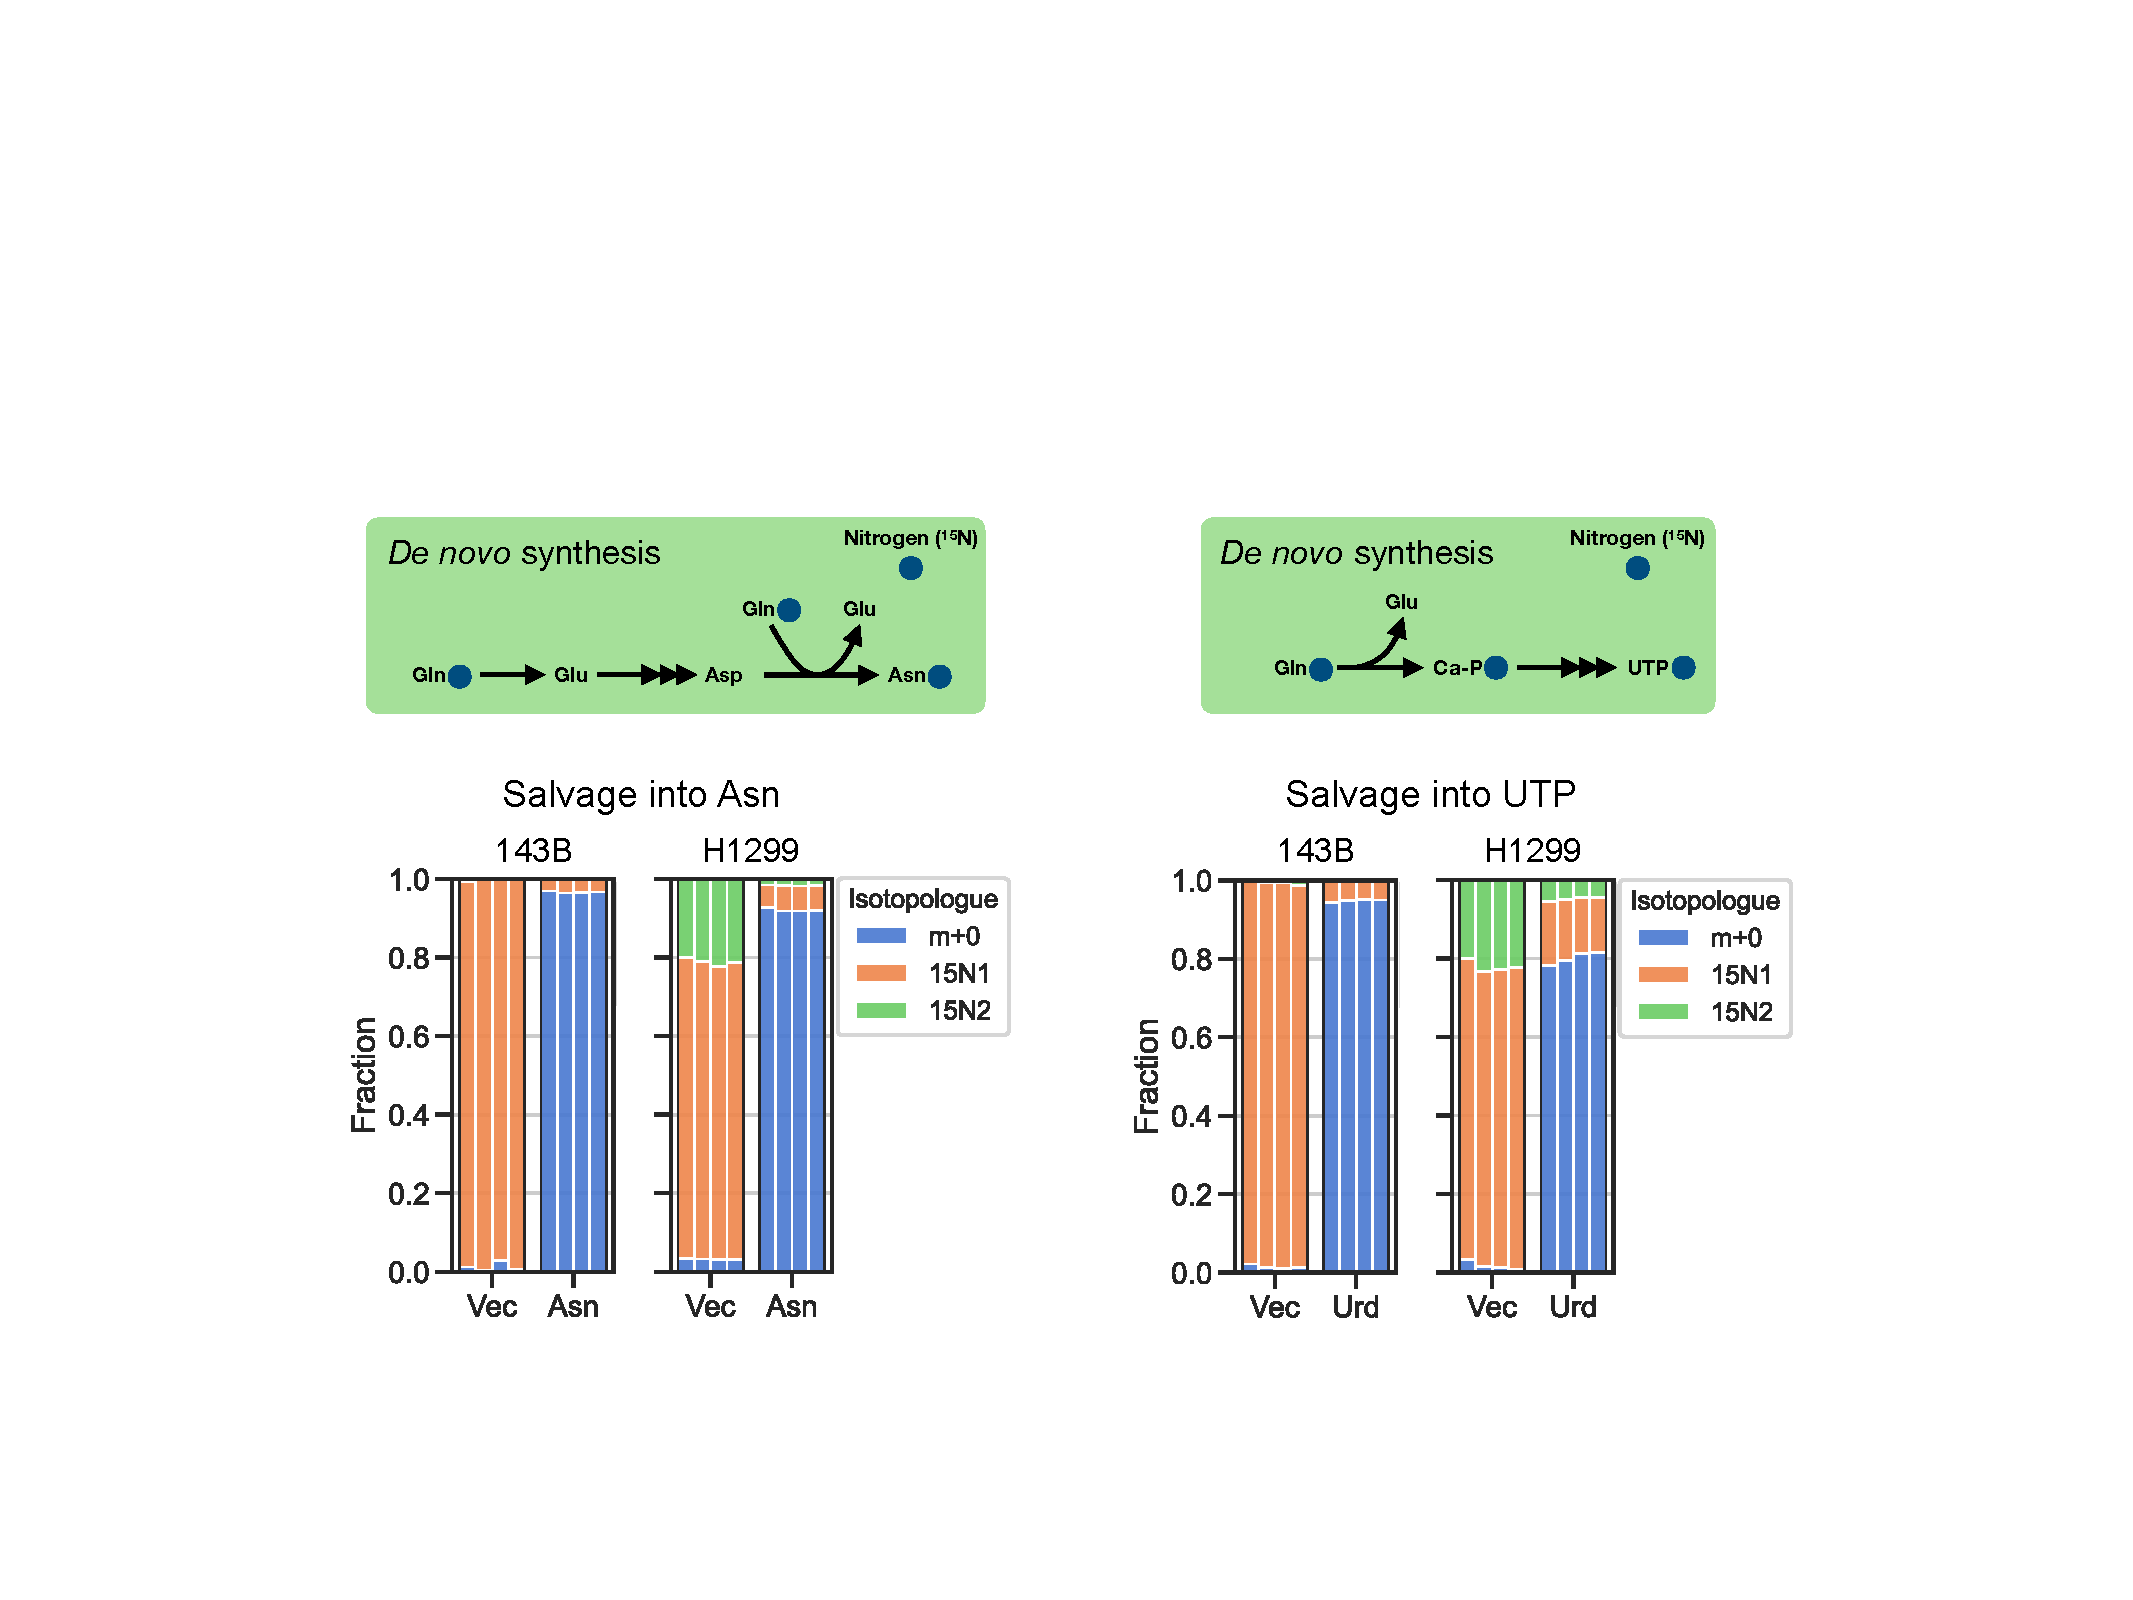
\includegraphics[width=0.8\textwidth]{figures/chap2/sal_frac_pyr-asn.pdf}
    \caption[Salvage into asparagine and pyrimidines]{
    ggg
    }
    \label{fig:ch2:sal_frac_pyr-asn}
\end{figure}









\begin{figure}
    \centering
    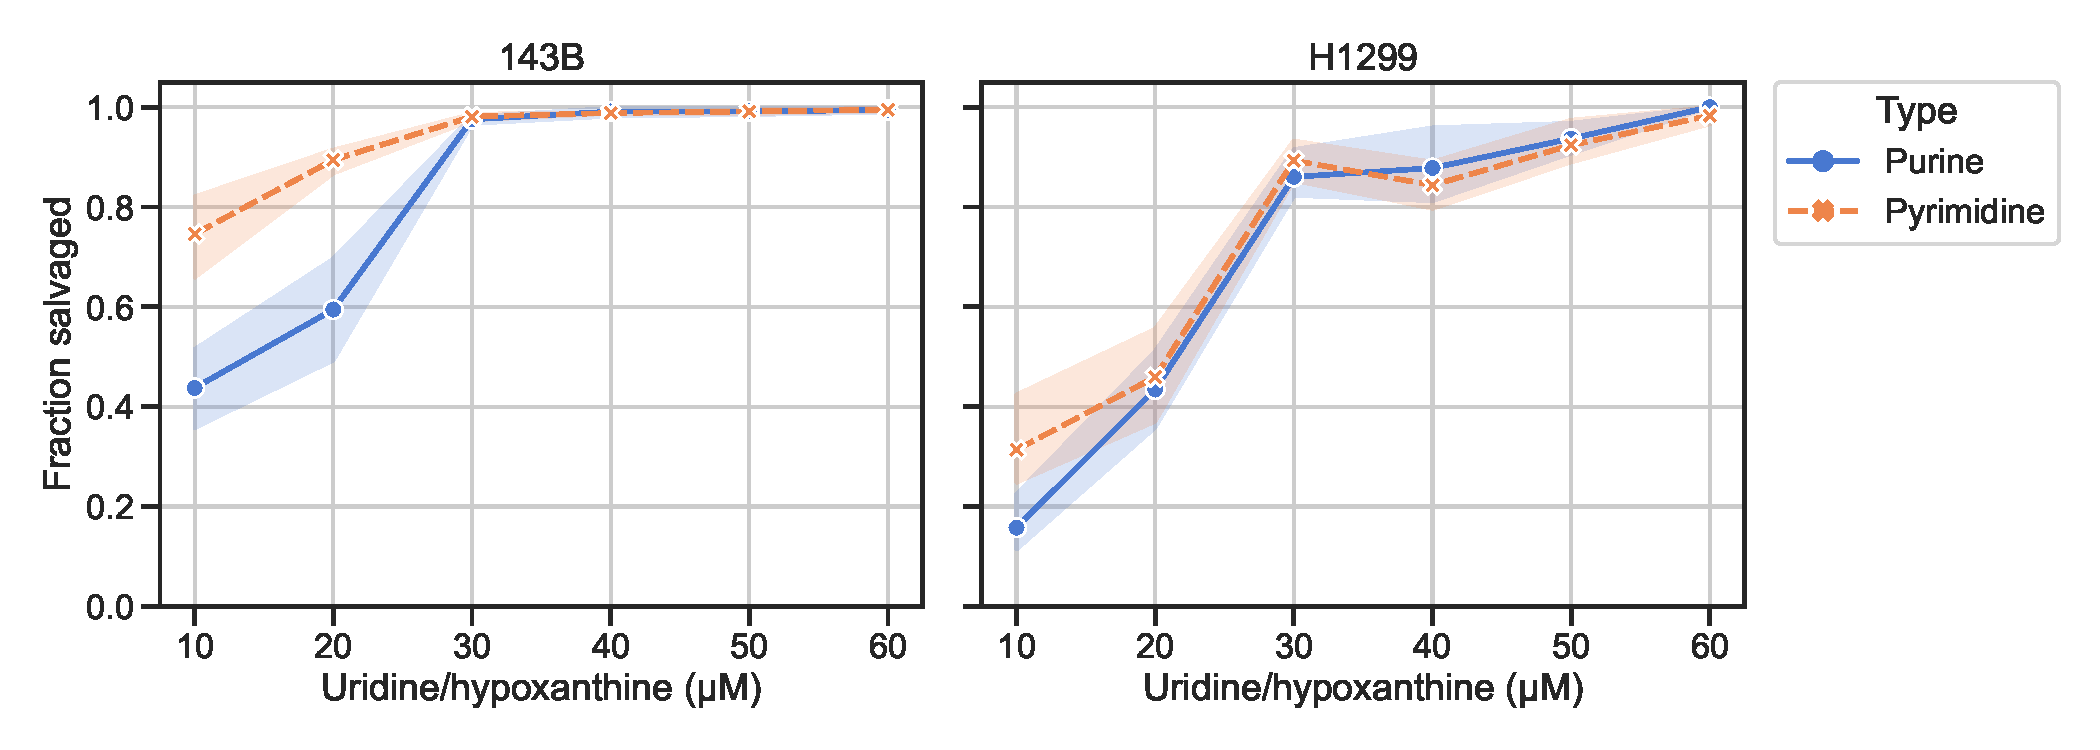
\includegraphics[width=0.95\textwidth]{figures/chap2/sal_frac_conc.pdf}
    \caption[Salvage as a function of Urd/Hpx concentration]{
    Fraction of purines (GDP, GMP, ADP and AMP) and pyrimidines (UDP, UMP, CDP and CMP) derived from salvage when 143B or H1299 cells are cultured in increasing concentrations of uridine/hypoxanthine.
    }
    \label{fig:ch2:sal_frac_conc}
\end{figure}







\section{Aspartate to proliferation curves}

%%% Experiments with individual components under "ETCrescue" folder in lab-work

%%% Experiments with H1299 (Metformin and Rotenone) and HT1080




\section{Integrated stress response}

Overlap between perturbations eliciting ISR by GCN2 and HRI \cite{Taniuchi2016-nc}









\section{Methods and Materials}

\subsection{Cell culture}
Cell lines were acquired from ATCC (143B, H1299, HT1080) and tested to be free from mycoplasma (MycoProbe, R\&D Systems).
Cells were maintained in Dulbecco’s Modified Eagle’s Medium (DMEM) (Gibco, 50-003-PB) supplemented with 3.7 g/L sodium bicarbonate (Sigma, S6297), 10\% fetal bovine serum (FBS) (Gibco, 26140079) and 1\% penicillin-streptomycin solution (Sigma, P4333).
Cells were incubated in a humidified incubator at 37°C with 5\% CO2.


\subsection{Western blots}
Protein lysates were harvested in RIPA buffer (Sigma, R0278) supplemented with Halt protease and phosphatase inhibitor cocktail (Fisher, PI78443) and 5 mM EDTA.
Protein concentration was determined using a bicinchoninic acid assay (Fisher, 23225) using bovine serum albumin (BSA) as a protein standard.
Equal amounts of protein were added to LDS sample buffer (ThermoFisher, B0008) and 5\% 2-Mercaptoethanol (Sigma, M3148), denatured at 95°C for 5 min, loaded onto 4–12\% SDS-polyacrylamide gels (Invitrogen, NW04122BOX) along with a prestained protein ladder (ThermoFisher, 26616) and run 35 min at 180V in MES buffer (ThermoFisher, B000202).
Proteins were dry transferred onto a 0.22 mm nitrocellulose membranes using the iBlot2 device (ThermoFisher, IB21001) with the P0 system setting and associated transfer stacks (Fisher, IB23001).
Membranes were blocked with 5\% bovine serum albumin; Sigma, A4503 in tris-buffered saline with 0.1\% Tween-20 (TBS-T) and incubated at 4°C overnight with the following antibodies:
anti-ATF4 (Cell Signaling, 11815S, 1:500),
anti-ASNS (Cell Signaling, 92479T, 1:1000),
anti-Phospho-eIF2alpha (Cell Signaling, 3398S, 1:500),
anti-eIF2alpha (Cell Signaling, 5324S, 1:500),
anti-Phospho-GCN2 (Cell Signaling, 94668S, 1:500),
anti-GCN2 (Cell Signaling, 3302S, 1:500),
anti-OMA1 (Cell Signaling, 95473, 1:1000),
anti-GADD34 (Proteintech, 10449-1-AP, 1:500),
anti-DARS2 (Proteintech, 13807-1-AP, 1:500),
anti-HRI (Sigma, HPA016496, 1:1000),
anti-FLAG (Sigma, F1804; 1:1000),
anti-SLC1A3 (Genetex, GTX20262; 1:500),
anti-GOT2 (Proteintech, 14800–1-AP, 1:750),
anti-GOT1 (Cell Signaling, 34423 S, 1:1000),
anti-Vinculin (Sigma, SAB4200729; 1:10,000) and anti-Tubulin (Sigma, T6199; 1:10,000).
Membranes were washed with TBS-T and the following secondary antibodies were added in blocking buffer: 800CW Goat anti-Mouse IgG (LiCOR, 926–32210; 1:15,000), 680RD Goat anti-Rabbit IgG (LiCOR, 926–68071; 1:15,000) and incubated for 1 hour.
Membranes were washed with TBS-T, incubated for 10 min in TBS-T, washed in deionized water and imaged on a LiCOR Odyssey Near-Infrared imaging system.


\subsection{Proliferation assays}
Cells were trypsinized (Corning, 25,051 CI), resuspended in seeding media, counted (Beckman Coulter Counter Multisizer 4) and seeded overnight onto 6/12/24-well dishes (Corning, 3516;3513:3524) with an initial seeding density of 10,000 cells/mL and a volume of 4, 2 and 1 mL, respectively.
After overnight incubation, 3–6 wells were counted for a starting cell count at the time of treatment.
Treatment was initiated either by media switch or by spike-in of drug/metabolite from a 20-50x stock.
Experiments were conducted in (both for seeding and treatment) DMEM without pyruvate (Corning 50–013-PB) supplemented with 3.7 g/L sodium bicarbonate 10\% dialyzed fetal bovine serum (FBS) (Sigma, F0392) and 1\% penicillin-streptomycin solution, with or without sodium pyruvate (Pyr) (Sigma, P8574),
2-ketobutyric acid (AKB) (Sigma, K401),
aspartate (Asp) (Sigma, A7219),
asparagine (Asn) (Sigma, A7094),
uridine (Urd) (Sigma, U3003), hypoxanthine (Cayman Chemical, 22254),
adenine (Ade) (Sigma, A2786),
guanine (Gua) (Sigma, 51030) or sodium formate (Sigma, 71539) with concentration noted when relevant.
Drug treatments included rotenone (Sigma, R8875),
metformin (Sigma, D150959),
atpenin A5 (Cayman Chemical, 11898; AdipoGen, AG-CN2-0110; Abcam, ab144194; or Enzo Life Sciences, ALX-380–313),
doxycycline hydrochloride (Sigma, D3447),
antimycin A (Sigma, A8674),
oligomycin A (Sigma, 495455),
GCN2iB (MedChemExpress, HY-112654),
FCCP (Cayman Chemical, 15218-10),
BAM15 (Cayman Chemical, 17811),
UCPH (HelloBio, HB0630) and DMSO vehicle (Sigma, D2650).
Cells were incubated in a humidified incubator at 37°C with 5\% CO2, then counted after 4–6 days.
Proliferation rate was reported as doublings per day and determined using the time and fold count difference between the starting and final counts and assuming a constant proliferation rate throughout the assay.


\subsection{Generation of nuclear RFP cell lines}
Nuclear RFP cell lines were generated using 1e5 transducing units of EF1A-nuclear RFP lentivirus (Cellomics Technology, PLV-10205-50) by spinfection.
Cells were seeded at 50\% confluency on 6 well dishes, lentivirus was added to fresh media with 8 µg/µL polybrene, then added to cells and followed by centrifugation (900g, 90 mins, 30°C).
Two days after infection, cells were sorted for high RFP expression using fluorescence-activated cell sorting (FACS).
High RFP cells were then expanded and single-cell cloned by limiting dilution, plating 0.5 cells/well on a 96 well plate.
Plates were then screened for RFP expression and localization using Incucyte S3 (Sartorius) and a suitable clone chosen, expanded, and used for all subsequent experiments.


\subsection{Incucyte measurements}
Proliferation assay using Incucyte



\subsection{Lentiviral production and stable cell line generation}
The following plasmids were obtained: pLenti6.3-V5 DEST\_SLC1A3 (DNASU Plasmid Repository), ATF4 reporter pXG237 (Addgene, 141281), pLHCX-gpASNase1 (Addgene, 121526) and pDONR221\_EGFP (Addgene, 25899).
ASNS was cloned by PCR from HEK293T reverse transcribed mRNA.
Genes were first cloned into entry vector pENTR1A (Fisher, A10462) using NEBuilder HiFI DNA Assembly Cloning Kit (New England BioLabs, E2621).
These donor constructs were then used to transfer their insert into destination vectors: pLX304-CMV-Blast (Addgene, 25890) or pLenti-CMV-Hygro (w117-1) (Addgene, 17454 a gift from Eric Campeau \& Paul Kaufman) using LR Clonase II (Fisher, 11791100).
Each plasmid sequence was verified by whole plasmid sequencing (Plasmidsaurus).
Lentivirus was generated by co-transfection of HEK293T cells with destination vector plasmid DNA and the packaging plasmids pMDLg/pRRE (Addgene, 12251), pRSV-Rev, (Addgene, 12253) and pMD2.G (Addgene, 12259) using FuGENE transfection reagent (Fisher, PRE2693) in DMEM (Fisher, MT10017CV) without FBS or penicillin-streptomycin.
The supernatant containing lentiviral particles was filtered through a 0.45 µM membrane (Fisher, 9720514) and was supplemented with 8 µg/µL polybrene (Sigma, TR-1003-G) prior to infection.
For infection, cells were seeded at 50\% confluency in 6 well dishes and centrifuged with lentivirus (900g, 90 mins, 30°C).
After 24 hours the media was replaced with fresh media and after 48 hours cells were treated with either 1 µg/mL blasticidin (Fisher, R21001) or 150 µg/mL hygromycin (Sigma, H7772-1G) and maintained in selection media until all uninfected control cells died.
After selection, cells were expanded and single-cell cloned by limiting dilution, plating 0.5 cells/well using 96 well plates.
These clones were expanded and screened by either western blot or presence of GFP or RFP signal using Incucyte S3 (Sartorius) to validate expression.
From this a single clone was chosen, expanded and used for all subsequent experiments.


\subsection{Generation of knockout cells}
Protocol and guide RNA generation was identical to that described in Hart et al. \cite{Hart2023-gp}.
Briefly, three chemically synthesized 2'-O-methyl 3’phosphorothioate-modified single guide RNA (sgRNA) sequences targeting the gene of interest were purchased (Synthego; table \ref{tab:ch2:guides}).
A pool of all three sgRNAs (or all six for GOT1/GOT2 double knockout) were resuspended in nuclease-free water, combined with SF buffer (Lonza, V4XC-2032), and sNLS-spCas9 (Aldevron, 9212).
200,000 H1299 cells were resuspended in the resulting solution containing ribonucleoprotein complexes (RNPs) and electroporated using a 4D-Nucleofector (Amaxa, Lonza).
Nucleofected cells were then expanded and single-cell cloned by limiting dilution by plating 0.5 cells/well in a 96 well plate.
Gene knockout was confirmed using western blots.

\begin{spacing}{1}
\begin{table}[ht]
\caption{\label{tab:ch2:guides}CRISPR guides.}
\begin{tabular}{|l|l|}
\hline
Gene & sgRNA   sequence (5’-3’) \\
\hline
GOT1 & \begin{tabular}[c]{@{}l@{}}\texttt{CAGUCAUCCGUGCGAUAUGC}\\\texttt{GCACGGAUGACUGCCAUCCC}\\\texttt{CGAUCUUCUCCAUCUGGGAA}\end{tabular} \\
\hline
GOT2 & \begin{tabular}[c]{@{}l@{}}\texttt{UUUCUCAUUUCAGCUCCUGG}\\\texttt{CGGACGCUAGGCAGAACGUA}\\\texttt{UCCUUCCACUGUUCCGGACG}\end{tabular} \\
\hline
OMA1 & \begin{tabular}[c]{@{}l@{}}\texttt{ACACAUUAGCAUCCACCUCA}\\\texttt{GAGUAAAUCAGUGUGACAGG}\\\texttt{GCCAACCCAAGAUGCCAGAA}\end{tabular} \\
\hline
HRI & \begin{tabular}[c]{@{}l@{}}\texttt{GUUUGCAACUGCAAAAGGGA}\\\texttt{UGAUGUUCCAGCAGAAAUCC}\\\texttt{CCAGCACCUUCACUUCCCGU}\end{tabular} \\
\hline
GCN2 & \begin{tabular}[c]{@{}l@{}}\texttt{AAAACUAAAUUGAUUUCAGG}\\\texttt{AGCUCGGUCAUCCUUGGCCA}\\\texttt{GAACUGGCCAAGAAACACUG}\end{tabular} \\
\hline
SLC25A10 & \begin{tabular}[c]{@{}l@{}}\texttt{GCAUCUGCAGACGCAGCAGG}\\\texttt{GCAACACCUUCUCGUGGAAG}\\\texttt{GAAGCUGCGCAUGACGGGCA}\end{tabular} \\
\hline
DARS2 & \begin{tabular}[c]{@{}l@{}}\texttt{ACAUAAAAUCUUCUUCACAG}\\\texttt{UGGUUAAGUCAGCUGUACAG}\\\texttt{GUGGAUGGAUUCAGUACCGA}\end{tabular} \\
\hline
\end{tabular}
\end{table}
\end{spacing}

\subsection{Polar metabolite extraction}
For polar metabolite extraction, a plate was move to ice and the media was thoroughly aspirated.
Wells were washed thrice with cold saline (Fisher, 23293184), 1 mL 80\% HPLC grade methanol in HPLC grade water was added, cells were scraped with the back of a P1000 pipet tip and transferred to Eppendorf tubes.
Tubes were centrifuged (17,000g, 15 mins, 4°C) and a fraction of the supernatant containing polar metabolites was transferred to a new centrifuge tube and placed in a centrivap until dry.
The fraction of supernatant transferred was adjusted to correspond to that extracted from a 1 µL cell volume e.g. 50\% was transferred if the total cell volume extracted from was 2 µL.
The total cell volume extracted from was determined by counting cells on a parallel plate using a coulter counter.
Dried samples were reconstituted with 40 µL 80\% HPLC grade methanol, containing internal standards if appropriate, and transferred to vials for measurement by LCMS.

\subsection{Media metabolite extraction}
For media metabolite extraction, 10 µL media was sampled, added to 990 µL 80\% HPLC grade methanol in HPLC grade water and incubated at -20°C for 30 min or until ready.
Tubes were centrifuged (17,000g, 15 mins, 4°C) and 400 µL of the supernatant containing media metabolites was transferred to a new centrifuge tube and placed in a centrivap until dry.
Dried samples were reconstituted with 40 µL 80\% HPLC grade methanol, containing internal standards if appropriate, and transferred to vials for measurement by LCMS.


\subsection{Absolute quantification by isotope dilution}
Dried samples were reconstituted with 40 µL 80\% HPLC grade methanol containing 5 µM U-\hCi, U-\hNi{} labelled canonical amino acid mix (Cambridge Isotope Laboratories, MSK-CAA-1) and transferred to vials for measurement by LCMS.
For pyrimidine nucleobase/nucleoside quantification a U-\hCi{} internal standard was made by partial hydrolysis (12 h in 6 M HCl at 90°C) of U-\hCi{} spirulina whole cells lyophilized powder (Cambridge Isotope Laboratories, CLM-8400-PK).
The peak area for each compound was divided by its labelled standard to derive the response ratio.
The response ratio was then mapped to a calibration curve to infer the compound concentration in the vial.
The sample concentration was calculated by correcting for each step introducing a dilution, for the intracellular concentrations this included using of the total cell volume.
To make the calibration curves a non-labelled amino acid mixture was made from an analytical amino acid standard without glutamine and asparagine (Sigma, A9906-1ML) and added glutamine (Sigma, 76523-100MG) and asparagine (Sigma, 51363-100MG) to match the concentration of the other amino acids.
For pyrimidine nucleobase/nucleoside quantification this pool was also mixed with equimolar uracil (Sigma, U1128), uridine (Sigma, U3003), 2′-deoxyuridine (Sigma, D5412), thymine (Sigma, T0376), cytosine (Sigma, C3506) and cytidine (Cayman Chemical, 29602).
Using this mix, three replicates of a 12 point 2-fold dilution series was made with a max concentration of 500 µM and a volume per dilution of 40 µL.
These were placed in a centrivap until dry and reconstituted with 40 µL 80\% HPLC grade methanol containing the appropriate isotopic internal standard and transferred to vials for measurement by LCMS.
The peak area for each compound was divided by its labelled standard to derive the response ratio, then the best fitting calibration curves for each compound were chosen among either linear, power or a second-degree polynomial.
Each calibration curve was manually inspected for proper fit and measurements below or above the concentration range of the dilution series were discarded.


\subsection{Liquid Chromatography-Mass Spectrometry (LCMS)}
Metabolite quantitation was performed using a Q Exactive HF-X Hybrid Quadrupole-Orbitrap Mass Spectrometer equipped with an Ion Max API source and H-ESI II probe, coupled to a Vanquish Flex Binary UHPLC system (Thermo Scientific).
Mass calibrations were completed at a minimum of every 5 days in both the positive and negative polarity modes using LTQ Velos ESI Calibration Solution (Pierce).
Polar Samples were chromatographically separated by injecting a sample volume of 1 µL into a SeQuant ZIC-pHILIC Polymeric column (2.1 x 150 mm 5 mM, EMD Millipore).
The flow rate was set to 150 mL/min, autosampler temperature set to 10°C, and column temperature set to 30°C.
Mobile Phase A consisted of 20 mM ammonium carbonate and 0.1\% (v/v) ammonium hydroxide, and Mobile Phase B consisted of 100\% acetonitrile.
The sample was gradient eluted (\%B) from the column as follows: 0-20 min.: linear gradient from 85\% to 20\% B; 20-24 min.: hold at 20\% B; 24-24.5 min.: linear gradient from 20\% to 85\% B; 24.5 min.-end: hold at 85\% B until equilibrated with ten column volumes.
Mobile Phase was directed into the ion source with the following parameters: sheath gas = 45, auxiliary gas = 15, sweep gas = 2, spray voltage = 2.9 kV in the negative mode or 3.5 kV in the positive mode, capillary temperature = 300°C, RF level = 40\%, auxiliary gas heater temperature = 325°C.
Mass detection was conducted with a resolution of 240,000 in full scan mode, with an AGC target of 3,000,000 and maximum injection time of 250 msec.
Metabolites were detected over a mass range of 70-850 m/z.
Quantitation of all metabolites was performed using Tracefinder 4.1 (Thermo Scientific) referencing an in-house metabolite standards library using ≤5 ppm mass error.
For samples subjected to stable isotope tracing, peak areas were natural abundance corrected with IsoCor \cite{Millard2019-hv}, using experimentally determined tracer purity values.



\subsection{Media uptake flux}
The cells were first passaged in DMEM with dialyzed FBS and the tracer and/or metabolites used during the uptake experiment.
For 143B GOT DKO cells expressing SLC1A3, 500 µM sodium aspartate was added to adjust intracellular aspartate levels.
For 143B WT cells, 100 µM U-\hCi{} Asn was added to achieve a steady-state label fraction in the proteome.
To start the experiment, cells were seeded on six well dishes at 1e5 cells/well.
On the next day fresh media was added and t=0 media samples were collected.
Then cells were incubated and subsequent media samples collected.
After the last media collection the residual media volume was quantified to correct for evaporation
For U-\hCi{} Asn tracing the labelling ratio was determined by extracting intracellular metabolites after the last media collection.
Two dishes were run in parallel and used for counting to determine proliferation rates and cell volume measurement using a coulter counter.

\subsubsection{Flux calculation}
Cell counts over time is assumed an exponential function ($y(t)$) with proliferation rate $K$ and cell count at $t=0$ being $y_0$:
\begin{equation}
    y(t) = y_0 2^{K t}
\end{equation}

Assuming amino acid uptake into a cell is constant, the uptake rate (also called influx) can be defined as the total molar uptake over a time range divided by the total area under the cell count curve of the same time range.
Formally, the flux of a compound $i$ is:
\begin{equation}
    F_i = \frac{n_i(t_1) - n_i(t_2)}{\int_{t_1}^{t_2} y(t) dt}
\end{equation}
With $F_i$ being the flux, $n_i(t)$ being the molar quantity of a compound $i$, and $t_1$ and $t_2$ being the first and second timepoint, respectively.

Using $\Delta$ to indicate the difference between $t_1$ and $t_2$, we can simplify the above:
\begin{equation}
    F_i = \frac{\Delta n_i}{\int_{t_1}^{t_2} y(t) dt} = \frac{\Delta n_i}{\frac{y_0 2^{K t_2}}{K\ \natlog(2)} - \frac{y_0 2^{K t_1}}{K\ \natlog(2)}} = \frac{\Delta n_i}{\frac{y_0 (2^{K t_2} - 2^{K t_1})}{K\ \natlog(2)}}
\end{equation}
The denominator is the area under the cell count curve from $t_1$ to $t_2$ and is sometimes referred to as ``cell hours'' because of its unit is time, typically hours.

Using cell hours it is possible to calculate the molar quantity taken up per cell per hour, typically as: $\frac{\text{fmol}}{\text{cell}\times h}$.
However, this makes it hard to compare across cell lines because of variability in cell size.
To fix this, simply redefine the problem from integrating the area under the cell count curve to the area under the cell volume curve.
The cell volume curve is defined using a volume per cell multiplier ($V_c$):
\begin{equation}
    V(t) = y(t) V_c = V_c y_0 2^{t K}
\end{equation}

Assuming cell volume is unchanged throughout the experiment, $V_c$ is a constant that is not integrated and we get:
\begin{equation}
    F_i = \frac{\Delta n_i}{\frac{V_c y_0 (2^{K t_2} - 2^{K t_1})}{K\ \natlog(2)}}
\label{eq:ch2:fl_vh}
\end{equation}
Since $V_c$ is a volume, we have a denominator with a typical unit of $\frac{L}{h}$.
We could call this ``volume hours'', and dividing a molar quantity onto this we typical get a unit of $\frac{\text{mM}}{h}$, which is comparable across cell lines with different sizes.

Sometimes it can be useful to convert the influx of a compound to its accumulated intracellular concentration, also referred to as total cell concentration.
The accumulated intracellular concentration of a compound can be understood intuitively as the total molar uptake divided by the total increase in cell volume.
To convert flux to total cell concentration for compound $i$ ($C_i$) observe the following rearrangement of equation \ref{eq:ch2:fl_vh}:
\begin{equation}
    F_i = K\ \natlog(2) \frac{\Delta n_i}{V_c y_0 (2^{K t_2} - 2^{K t_1})}
\end{equation}
The fraction is the total cell concentration for compound $i$ and thus we have:
\begin{equation}
    F_i = K\ \natlog(2) C_i => C_i = \frac{F_i}{K\ \natlog(2)}
\end{equation}


\subsubsection{Net asparagine consumption}
Human cells do not have any appreciable asparagine deaminase activity \cite{Sullivan2018-gz} and thus asparagine is a terminal metabolite that does not get converted or used as a substrate in other metabolic reactions.
This makes the asparagine fluxes suitable for isotope tracing if we make the explicit assumption is that asparagine can be generated from synthesis using aspartate but not recycled back.
Figure \ref{fig:ch2:asn_Jprot} shows the net asparagine fluxes when U-\hCi{} labelled Asn is added to the media.
Each net flux is the sum of fluxes in both directions e.g. U-\hCi{} Asn is net influxed because it is consumed while unlabelled Asn is net effluxed because it is absent from media at the initial conditions.

Influx and efflux can be measured by media sampling and using the ratio of labelled to unlabelled Asn inside the cell, the remaining fluxes can be solved.
Observe that the labelling ratio is defined by the influx, efflux and synthesis flux:
\begin{equation}
    \frac{\UAsn}{\Asn} = \frac{\Flin}{\Flsyn - \Flout}
\end{equation}

Isolate synthesis flux:
\begin{equation}
    \Flsyn = \frac{\Asn}{\UAsn} \Flin + \Flout
\label{eq:ch2:Jsyn}
\end{equation}

Introduce flux balance:
\begin{equation}
    \Flin + \Flsyn = \Flprot + \Flout => \Flprot = \Flin + (\Flsyn - \Flout)
\end{equation}

Isolate the flux of Asn deposition into protein ($\Flprot$) and insert $\Flsyn$ from equation \ref{eq:ch2:Jsyn}:
\begin{equation}
    \Flprot = \Flin + \left( \frac{\Asn}{\UAsn} \Flin + \Flout - \Flout \right)
\end{equation}

Simplify:
\begin{equation}
    \Flprot = \Flin \left( 1 + \frac{\Asn}{\UAsn} \right)
\label{eq:ch2:Jprot}
\end{equation}






\subsection{Acid hydrolysis}





Two 12W plates seeded in parallel (DMEM dia. FBS)
At 40-90\% confluency harvest by washing four times with saline
Count one plate
On the other plate add 1 mL 6M HCl to 5 wells, seal the plate and perform acid hydrolysis at 90C in incubator for 20h
Move hydrolysate to 2 mL tubes then wash the well thrice with 1 mL water and collect it in the same tube
Dry the hydrolysate
Add 0.5 mL 6M HCl to each tube and incubate another 48h at 90C, then dry
Reconstitute in 0.5 mL 6M HCl and aliquot 2 tubes with 10k cells and 2 tubes with 40k cells and dry.
Reconstitute the two 10k tubes with 1 mL water, move to a fresh tube, dry and reconstitute these with 40 uL SE+CAAv2 and run standard LCMS
Water reconstitution is an attempt to get rid of the plastic/glue soluble in HCl
Using uracil as a control (should be in the same range regardless of scraping or on plate hydrolysis)
% Sigma	84429-10X2ML	HCl for amino acid analysis






\subsection{Nitrogen-15 tracing}

\subsubsection{Salvage fraction of individual components}
The fractional contribution of individual components into their respective aspartate consuming fates was determined in 143B and H1299 cells for the salvageable metabolites asparagine (Asn), uridine (Urd), hypoxanthine (Hpx), adenine (Ade) and guanine (Gua) along with a vehicle treatment (Vec).
The salvageable metabolites were spiked-in from a 20x stock solution to achieve a final concentration of: 500 µM Asn, 200 µM Urd, 100 µM Hpx, 100 µM Ade or 100 µM Gua.
The fraction of salvage was determined by stable isotope tracing, performed using both Gln amide\=/\hNi{} (Cambridge Isotope Laboratories, NLM-557-PK) and Gln alpha\=/\hNi{} (Cambridge Isotope Laboratories, NLM-1016-PK) in separate reactions and added to DMEM without glucose, glutamine, pyruvate and phenol red (Sigma, D5030) supplemented with 10\% dialyzed FBS, 1\% penicillin-streptomycin, 25 mM glucose (Sigma, G7528).
The combination of cell lines, salvageable metabolites and tracers gave 2x6x2=24 conditions which were labelled to steady-state by culturing for four passages with a 1/20 split at each passage.
At the end of the last passage each condition was split into four technical replicates and plated on 24 well dishes (Corning, 3524).
Upon reaching confluency, polar metabolites were extracted and submitted to LCMS with the above described technique.

\subsubsection{Salvage fraction as a function of concentration}
Seeded H1299 and 143B cells at 5,000 and 10,000 cells/well on a 6-well dish in DMEM containing Gln amide\=/\hNi{} as described above.
Then added an equimolar mix of hypoxanthine and uridine from a 40x stock to a final concentration of 10, 20, 30, 40, 50, 60 µM in each of the 6 wells.
Fresh media was then added every four days and upon reaching confluency, polar metabolites were extracted and submitted to LCMS with the above described technique.








 % Molecular mechanisms of aspartate limitation

% Asp-sensor manuscript:
\chapter{Robust method for measuring aminoacylation through tRNA-seq}
This chapter is related to the paper: "[insert title here]" [insert reference here].
This paper describes a method for quantifying tRNA aminoacylation levels by making several improvements and combining the best of previous tRNA-seq methods.
The method is then tested using realistic sample conditions and an improved data processing strategy is described and tested.
All the essential findings of this chapter are described in the publication, and thus this should be preferred for most practical applications.
However, the publication focuses on the elements of method development that work and largely omits observations from experiments that failed.
I shall here correct this bias towards successful experiments, add new observations and interpretations, expand the background and discuss the many trade offs and pitfalls.


\section{Background}
Basic background like:
Purpose (protein synthesis).
Transfer RNA (tRNA).
Abundance compared to total RNA.
Length and sequencing similarity.
Transcripts of the same codon and copy number.

Transcription, intron splicing and CCA addition.
Modifications and their purpose (wobble, decoding etc.).
Compartmentalization (cyto, mito, chloroplasts)

Secondary structure.
Discriminator base.

Aminoacylation, enzyme specificity and ester bond stability.



\begin{figure}
     \centering
     \begin{subfigure}[b]{0.4\textwidth}
         \centering
         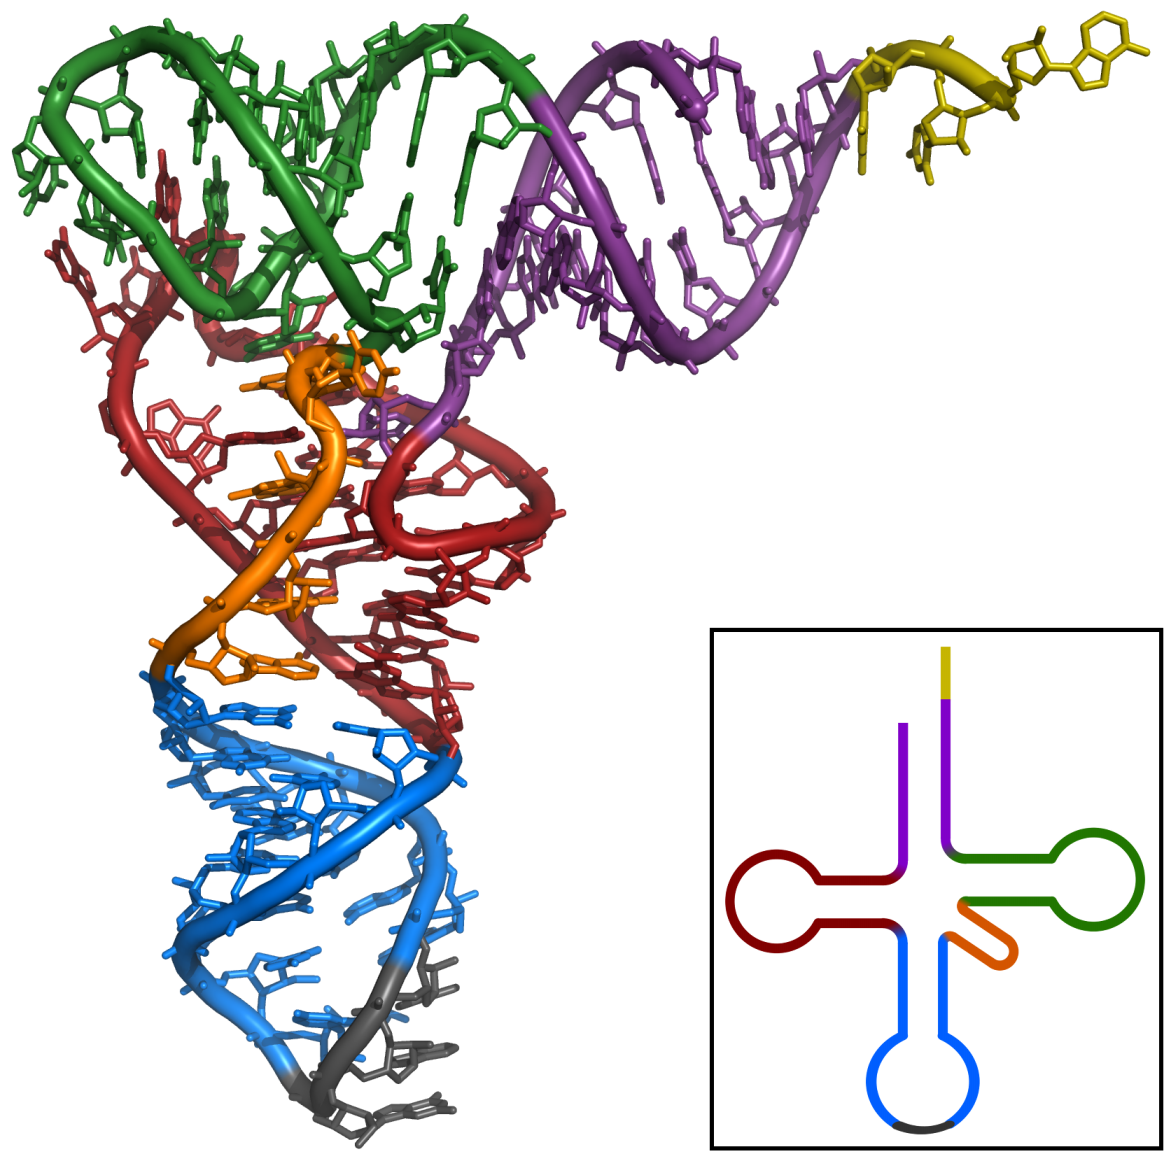
\includegraphics[width=\textwidth]{figures/chap3/TRNA-Phe_yeast_1ehz.png}
         \caption{}
         \label{fig:tRNA_3d_struct}
     \end{subfigure}
     \hfill
     \begin{subfigure}[b]{0.3\textwidth}
         \centering
         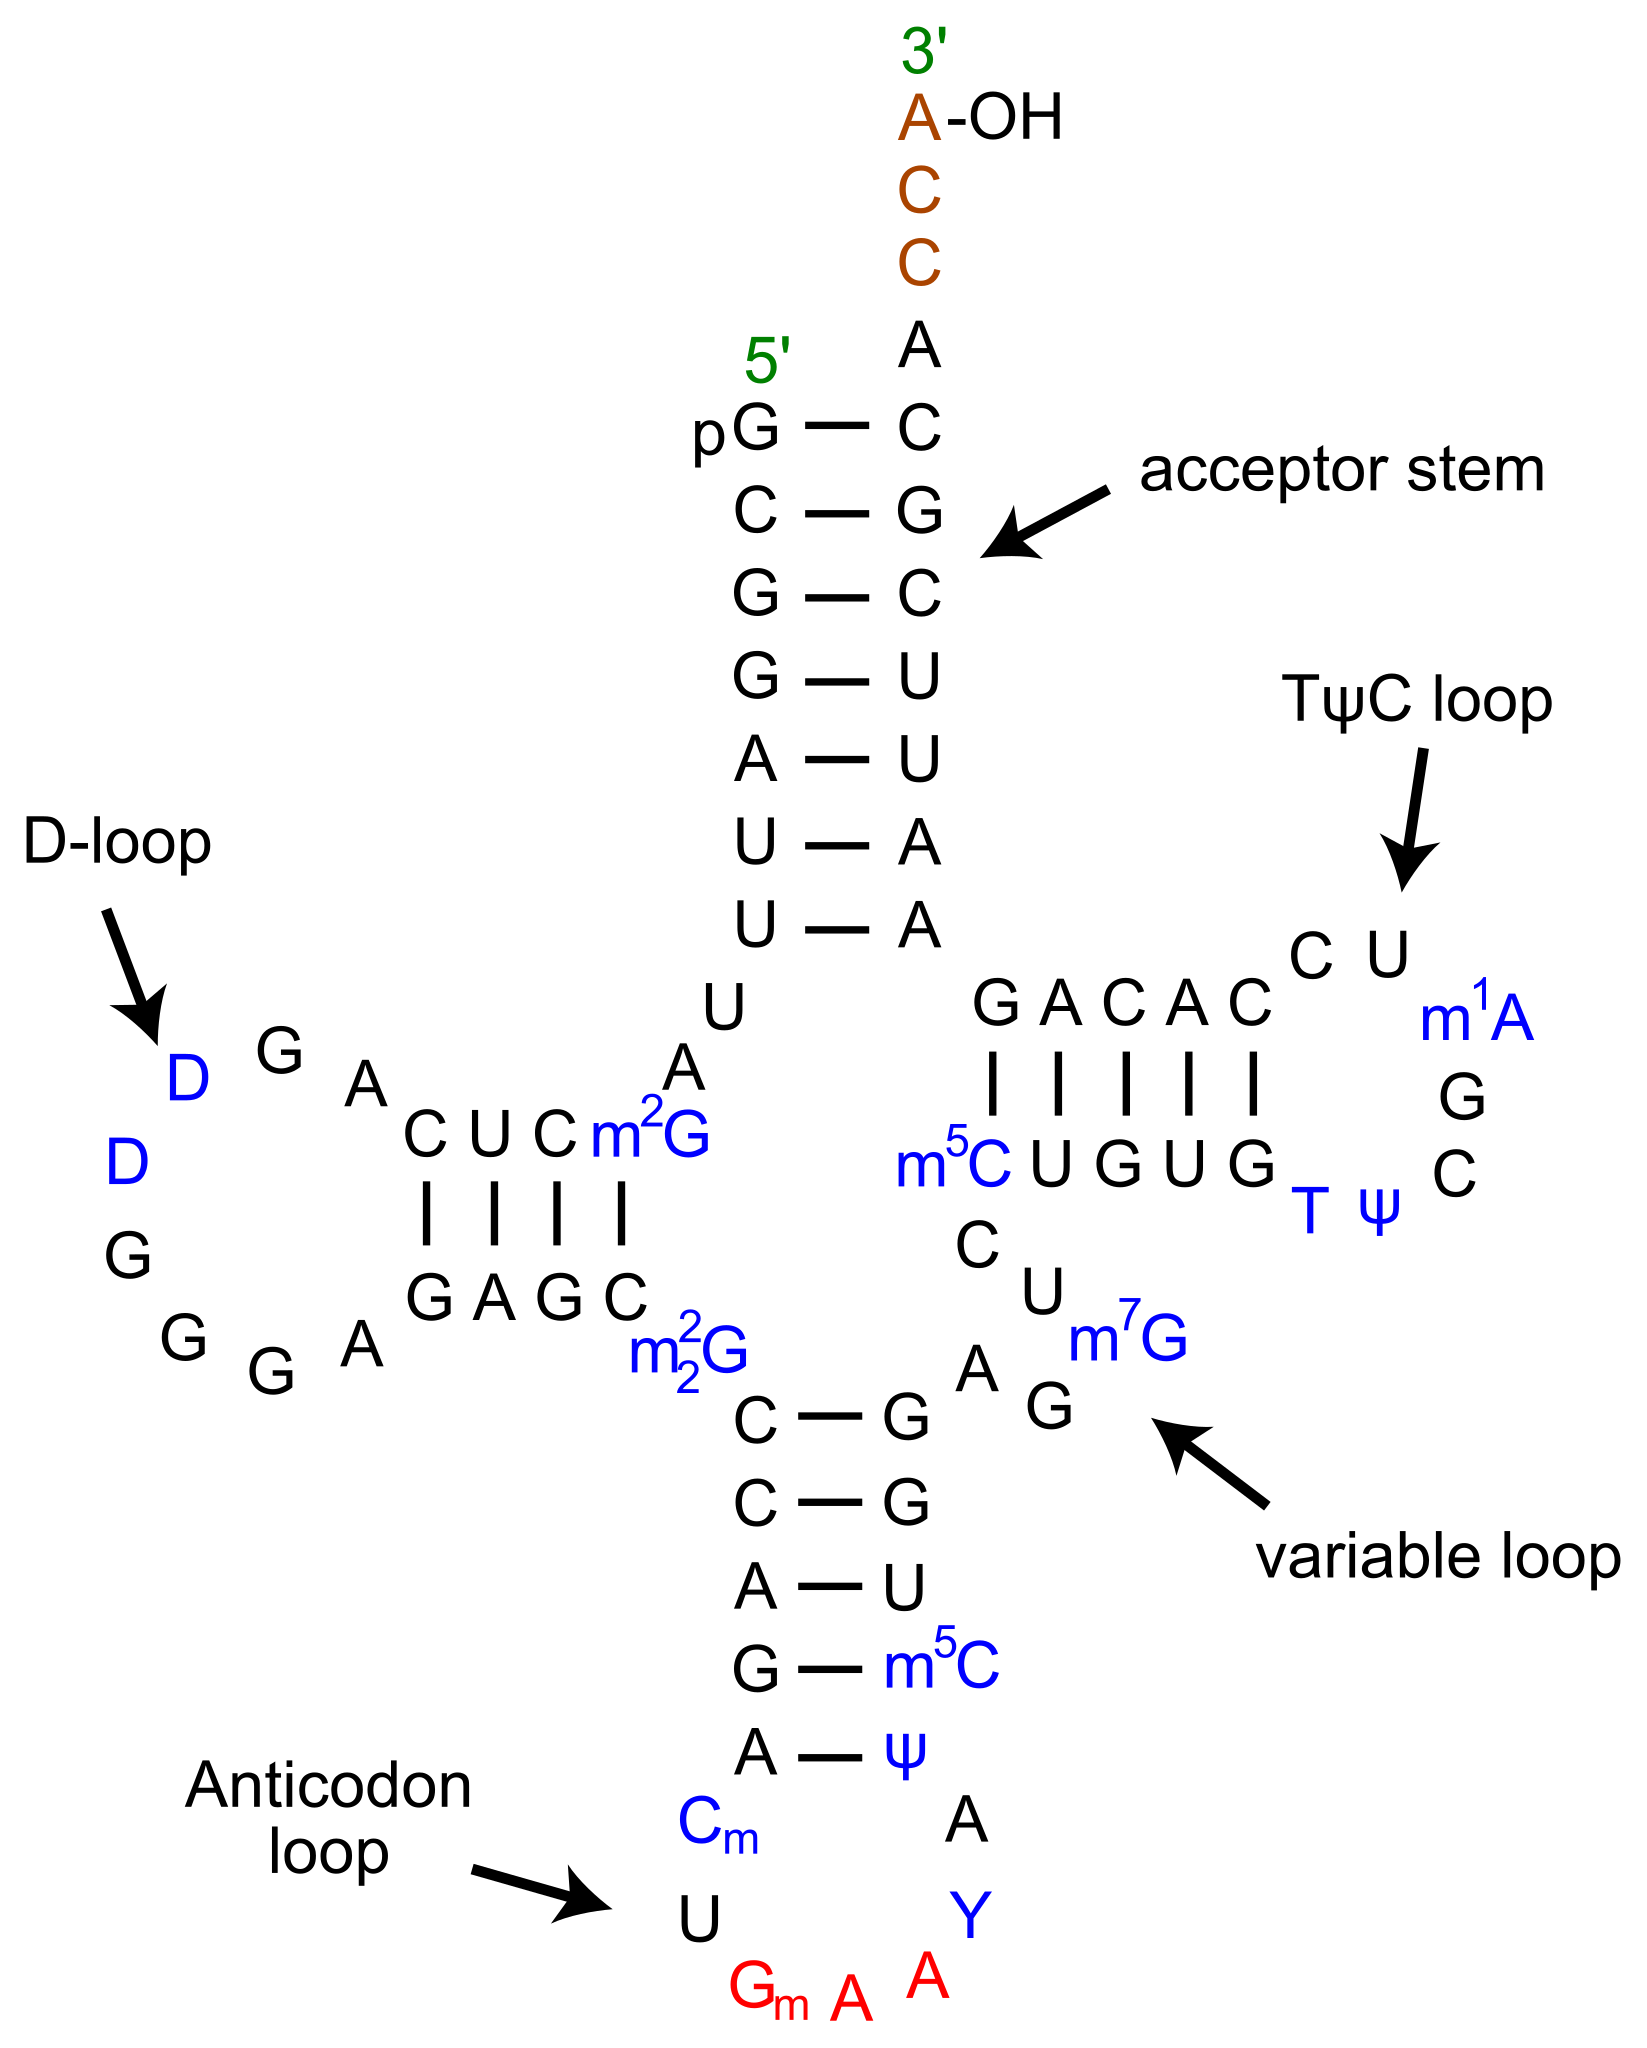
\includegraphics[width=\textwidth]{figures/chap3/TRNA-Phe_yeast_en.png}
         \caption{}
         \label{fig:tRNA_2d_struct}
     \end{subfigure}
     \hfill
     \begin{subfigure}[b]{0.2\textwidth}
         \centering
         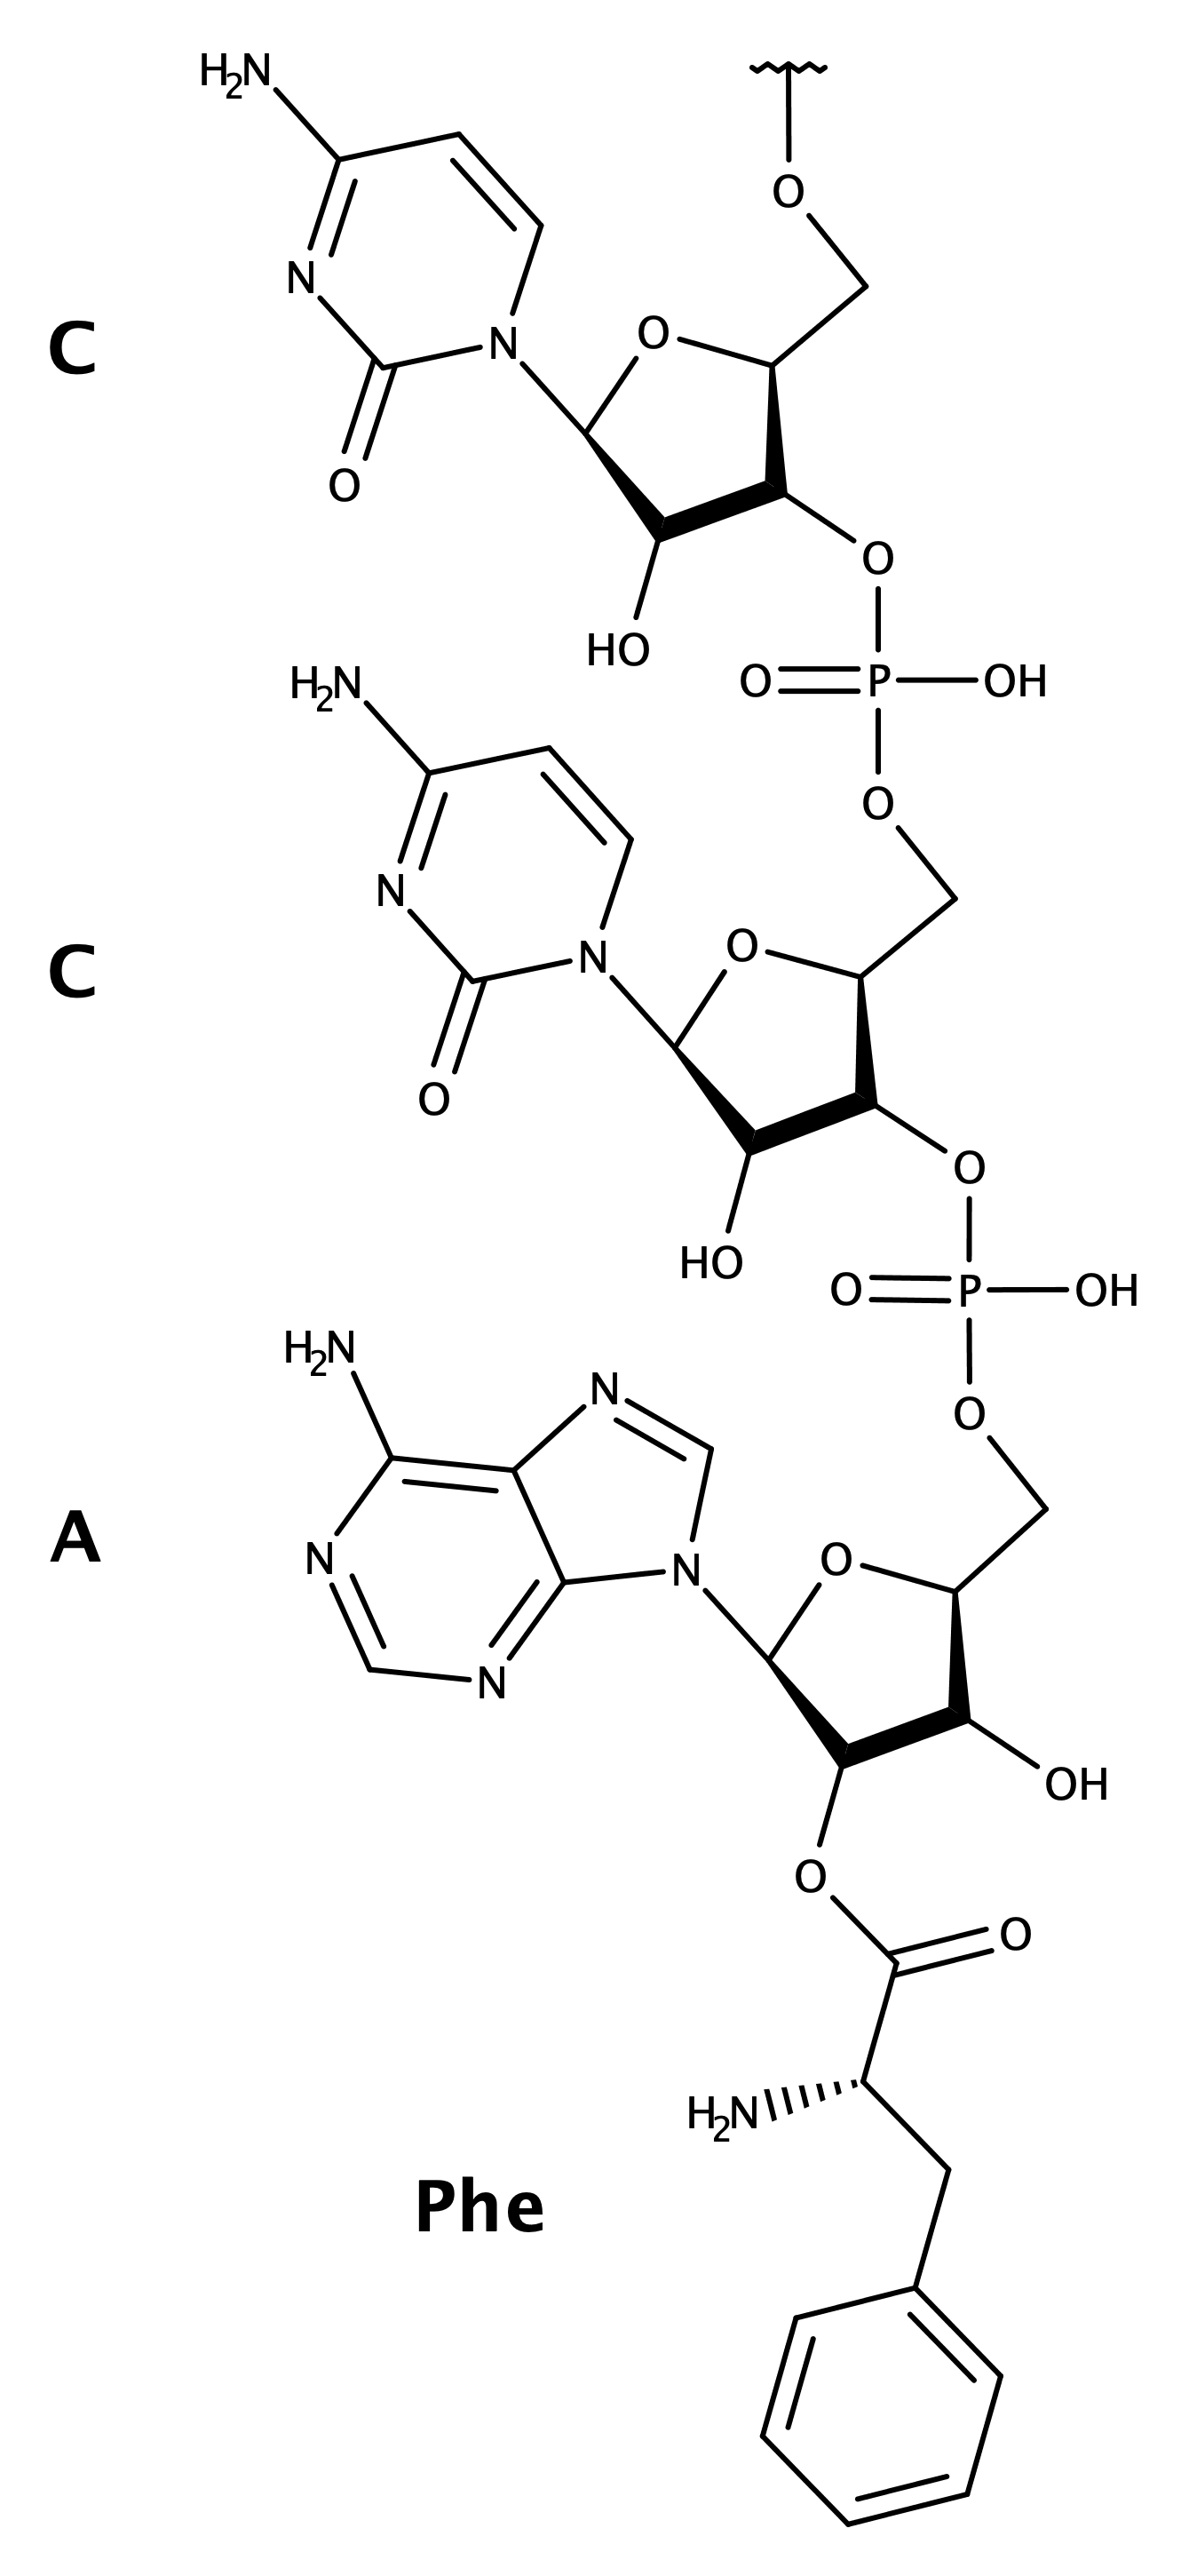
\includegraphics[width=\textwidth]{figures/chap3/CCA_Phe.png}
         \caption{}
         \label{fig:tRNA_CCAester}
     \end{subfigure}
        \caption{
        (a) Three dimensional structure of a tRNA colored by secondary structure elements shown in the insert, (b) secondary structure of a tRNA with names of the structural elements and some common base modifications, (c) the 3' CCA of a tRNA aminoacylated with phenylalanine.
        (a) and (b) from Yikrazuul, \href{https://creativecommons.org/licenses/by-sa/3.0}{CC BY-SA 3.0}, via Wikimedia Commons.
        }
\end{figure}





\begin{figure}
    \centering
    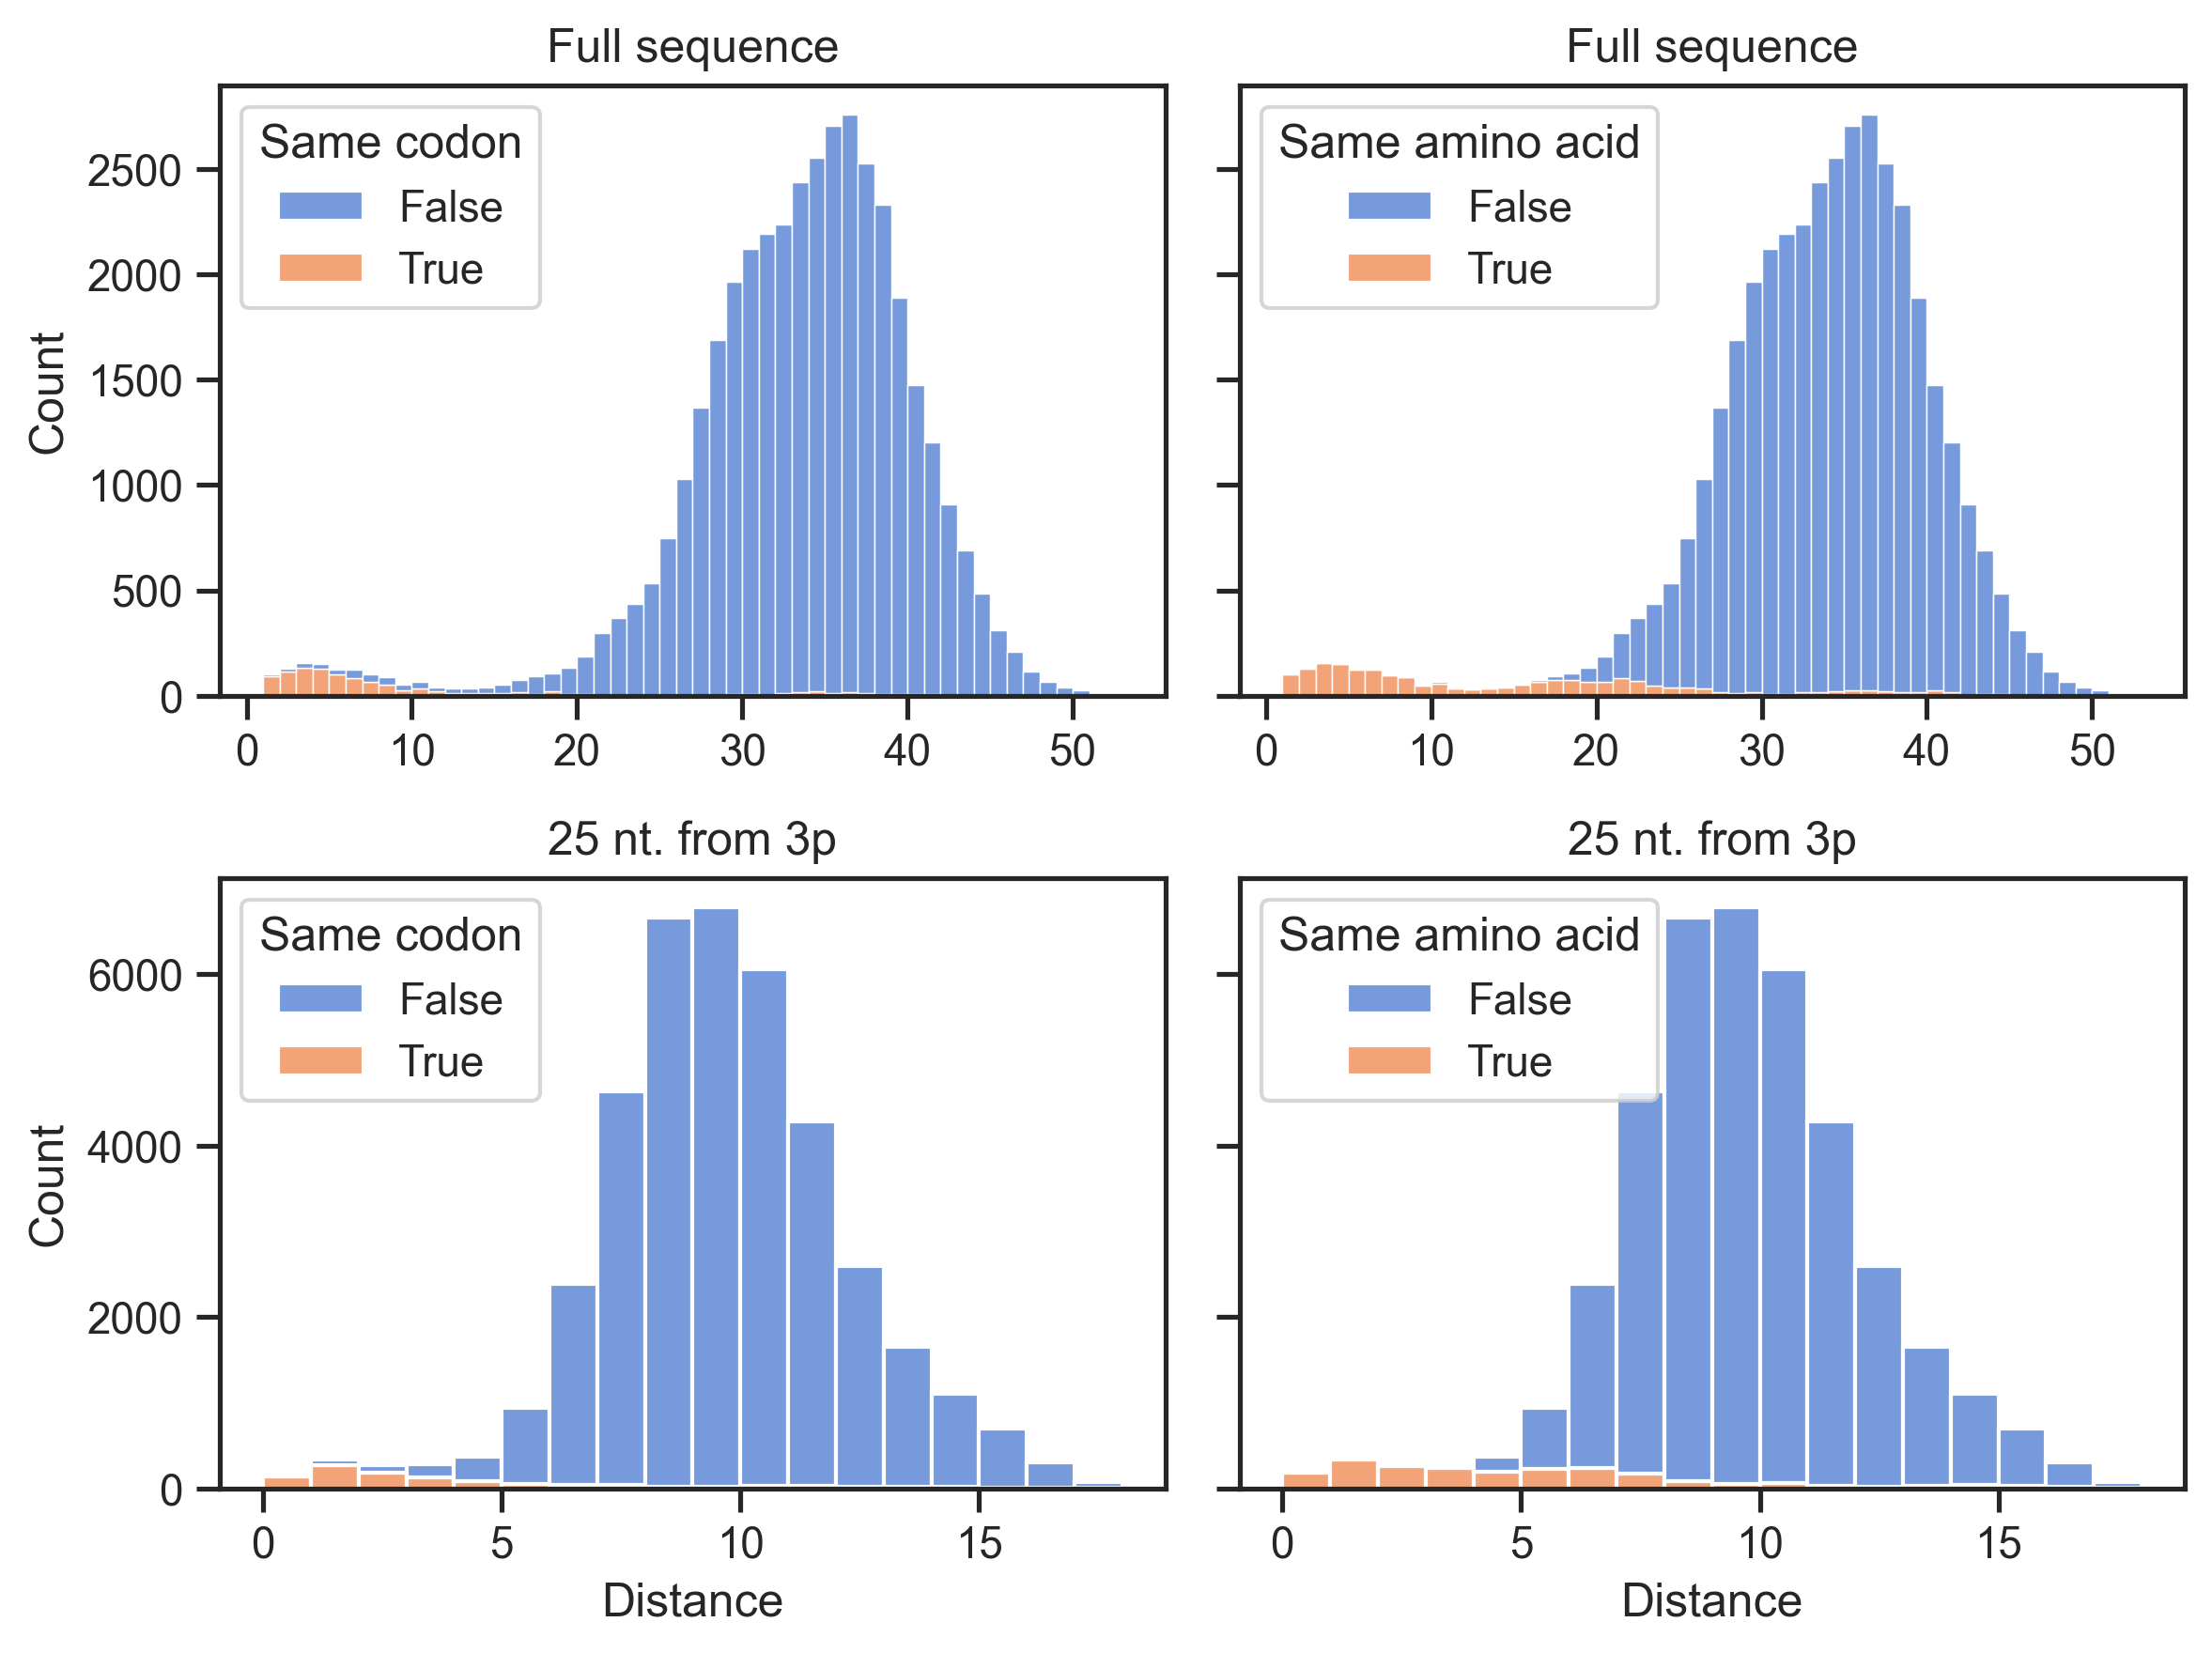
\includegraphics[width=\textwidth]{figures/chap3/tRNA_dist_hist.png}
    \caption{Histogram of the distances between tRNA transcripts after pairwise Needleman–Wunsch alignment. Distance is counted as the number of mismatches and gaps. The top row shows full sequence transcripts, the bottom row shows the last 25 nt. of each transcript. Distances are broken down by being between transcripts of the same codon or not, and same amino acid or not. Source: krdav Github \href{https://github.com/krdav/thesis_plotting/blob/main/tRNA_stats/plot_data.ipynb}{thesis\_plotting/tRNA\_stats}}
    \label{fig:dist_hist}
\end{figure}




\begin{table}[!htb]
\begin{tabular}{|l|p{0.85\textwidth}|}
\hline
Length & tRNAs \\ \hline
62     & m-Ser-AGC \\ \hline
68     & m-Arg-CGA \\ \hline
69     & m-Cys-UGC, m-Thr-ACA, m-Tyr-UAC \\ \hline
71     & m-Met-AUG, m-Trp-UGA, m-Pro-CCA, m-Gly-GGA, m-Asp-GAC \\ \hline
72     & m-Ser-UCA, m-Val-GUA, m-His-CAC, m-Ile-AUC, m-Glu-GAA, m-Ala-GCA \\ \hline
73     & c-Cys-UGC, m-Lys-AAA \\ \hline
74     & m-Phe-UUC, c-Gly-GGC, m-Leu-CUA, c-Ala-GCA, c-Gly-GGG \\ \hline
75     & c-Gln-CAG, c-Tyr-UAC, c-Ala-GCG, c-Ala-GCA, c-Gly-GGA, c-Pro-CCA,   c-Gln-CAA, c-Glu-GAG, c-Pro-CCU, c-Thr-ACA, c-Val-GUU, m-Gln-CAA, c-Asp-GAC,   c-Ala-GCU, c-Pro-CCG, c-Thr-ACG, c-His-CAC, c-Glu-GAA, c-Cys-UGC, c-Trp-UGG,   c-iMet-AUG \\ \hline
76     & c-Val-GUA, c-Arg-AGG, c-Tyr-UAU, c-Val-GUG, c-Ala-GCU, c-Tyr-UAC,   c-Arg-CGG, c-Met-AUG, m-Asn-AAC, c-Cys-UGC, c-Lys-AAG, c-Val-GUU, c-Arg-CGU,   c-Arg-CGA, c-Lys-AAA, c-Thr-ACA, c-Arg-AGA, c-Phe-UUC \\ \hline
77     & c-Thr-ACU, c-Ile-AUU, c-Ile-AUC, c-Lys-AAG, c-Asn-AAC, c-Leu-UUG,   c-Thr-ACA, c-Thr-ACG, c-Arg-AGA, c-Phe-UUC, c-Ile-AUA \\ \hline
78     & m-Leu-UUA, c-Asn-AAC \\ \hline
85     & c-Ser-UCG, c-Leu-CUU, c-Ser-AGC, c-Ser-UCU, c-Leu-CUA, c-Ser-UCA \\ \hline
86     & c-Leu-UUA, c-Leu-UUG, c-Leu-CUG \\ \hline
87     & c-Ser-AGC, c-Leu-UUG \\ \hline
90     & c-SeC-UGA \\ \hline
\end{tabular}
\caption{Mature human tRNA transcript lengths and the distribution among amino acids and codons. The tRNA column is populated with entries formatted as [cyto/mito]-[amino acid]-[codon] with [cyto/mito] indicated by c/m, [amino acid] indicated by the three letter amino acid code. Source: krdav Github \href{https://github.com/krdav/thesis_plotting/blob/main/tRNA_stats/plot_data.ipynb}{thesis\_plotting/tRNA\_stats}}
\end{table}
















\section{Quantifying aminoacylation}

Quantification of \textit{in vivo} transfer RNA (tRNA) aminoacylation is complicated by the many, highly similar, tRNA transcripts.
It was first with Northern blotting that tRNA transcripts could be resolved with sufficient resolution.
Aminoacylation can then be resolved by differential migration during electrophoresis and following probe quantification the level of aminoacylation, or charge, can be calculated \cite{Ho1987-ug, Varshney1991-zp, Stenum2017-wn}.





Multiple methods for quantifying aminoacylation these are...


\subsection{Northern blotting}
qwerty

\subsection{tRNA-seq}
Overview of the tRNA-seq methods.
Overview of the periodate-cleavage reaction.
Briefly, mention the array based tech introduced right before RNAseq.
Transition into giving an overview of each major advance in the methods.

\subsubsection{Zheng 2015}
Tao Pan RNAseq.
Extended by Evans 2017 to measure aminoacylation
\cite{Zheng2015-kj}


\subsubsection{Shigematsu 2017}
YAMAT seq


\subsubsection{Behrens 2021}
ghjm

\subsubsection{Others}
Here described other minor methodological advances/differences.
E.g. Wang [specifically amplified by GGT-ending primer during]







\subsection{The Malaprade-elimination reaction}
Dig deep into this reaction, the previous use, the chemistry etc.
This facilitates the discrimination between aminoacylated and unaminoacylated tRNA.
First used in Evans 2017, heavily inspired by the previous array based paper from Tao Pan's group.


\subsection{A lack of quantification rigor}
qwerty




\section{Strategy to improve tRNA-seq based aminoacylation quantification}


\section{Data processing}

\subsection{The alignment problem}
Blob on alignment:

* Maybe turn this into a wider discussion of annotation strategies and why it might be optimal to use masked sequences because this applies the least number of assumptions. A positional gap penalty would also help in that regard. HMM would be very strong but also would also make some assumptions about the modified sites that could be problematic in different contexts e.g. the HMM is fitted on data with a particular position always is modified but then in a biological context this modification is lost.
* Advantages: formalized model that calculated probabilities, can model site interactions, can model gaps and RT stops.
Modeling RT stops could be problematic though since it could easily vary depending on RT conditions, polymerases etc.
* Disadvantage: very slow, probably has to be refitted for new datasets because of slightly different RT conditions, also has to be refitted to take into account any biological changes in modification penetrance
* Pick a subset of reads with long alignments where the top scoring reference is several score points away from the runner up.
* Use these sequences to make an HMM for each annotation
* Run the HMMs on all sequences and calculate the annotation probability without the RT fall-off.
* Select all the sequences with an annotation with high HMM probability * away from the second best annotation.
* Refit the HMMs on these sequences.
* Run the HMMs on all sequences and calculate the annotation probability, this time with the RT fall-off included.
* Select sequences and refit HMM.
* Perform enough iterations to converge.





\section{Results}


\section{Methods}

\section{Discussion}



 % An engineered biosensor enables dynamic aspartate measurements in living cells

% Describe all things relevant to understand tRNA-Seq method:
\chapter{First degree dependence of aspartate for cell proliferation}

Closing chapter, dumping all the shitty unpublished data here.

\section{Introduction}
More blaa % Introduction to tRNA biology

% tRNA-Seq manuscript:
\chapter{Robust method for measuring aminoacylation through tRNA-seq}
Insert tRNA-Seq manuscript here.
 % Robust method for measuring aminoacylation through tRNA-seq

% Future directions:
\chapter{Future directions}

Closing chapter 

\section{Introduction}
More blaa

Cell size the nucleotide imbalance hypothesis.
%%% See "ETCrescue" folder under lab-work



\begin{figure}
    \centering
    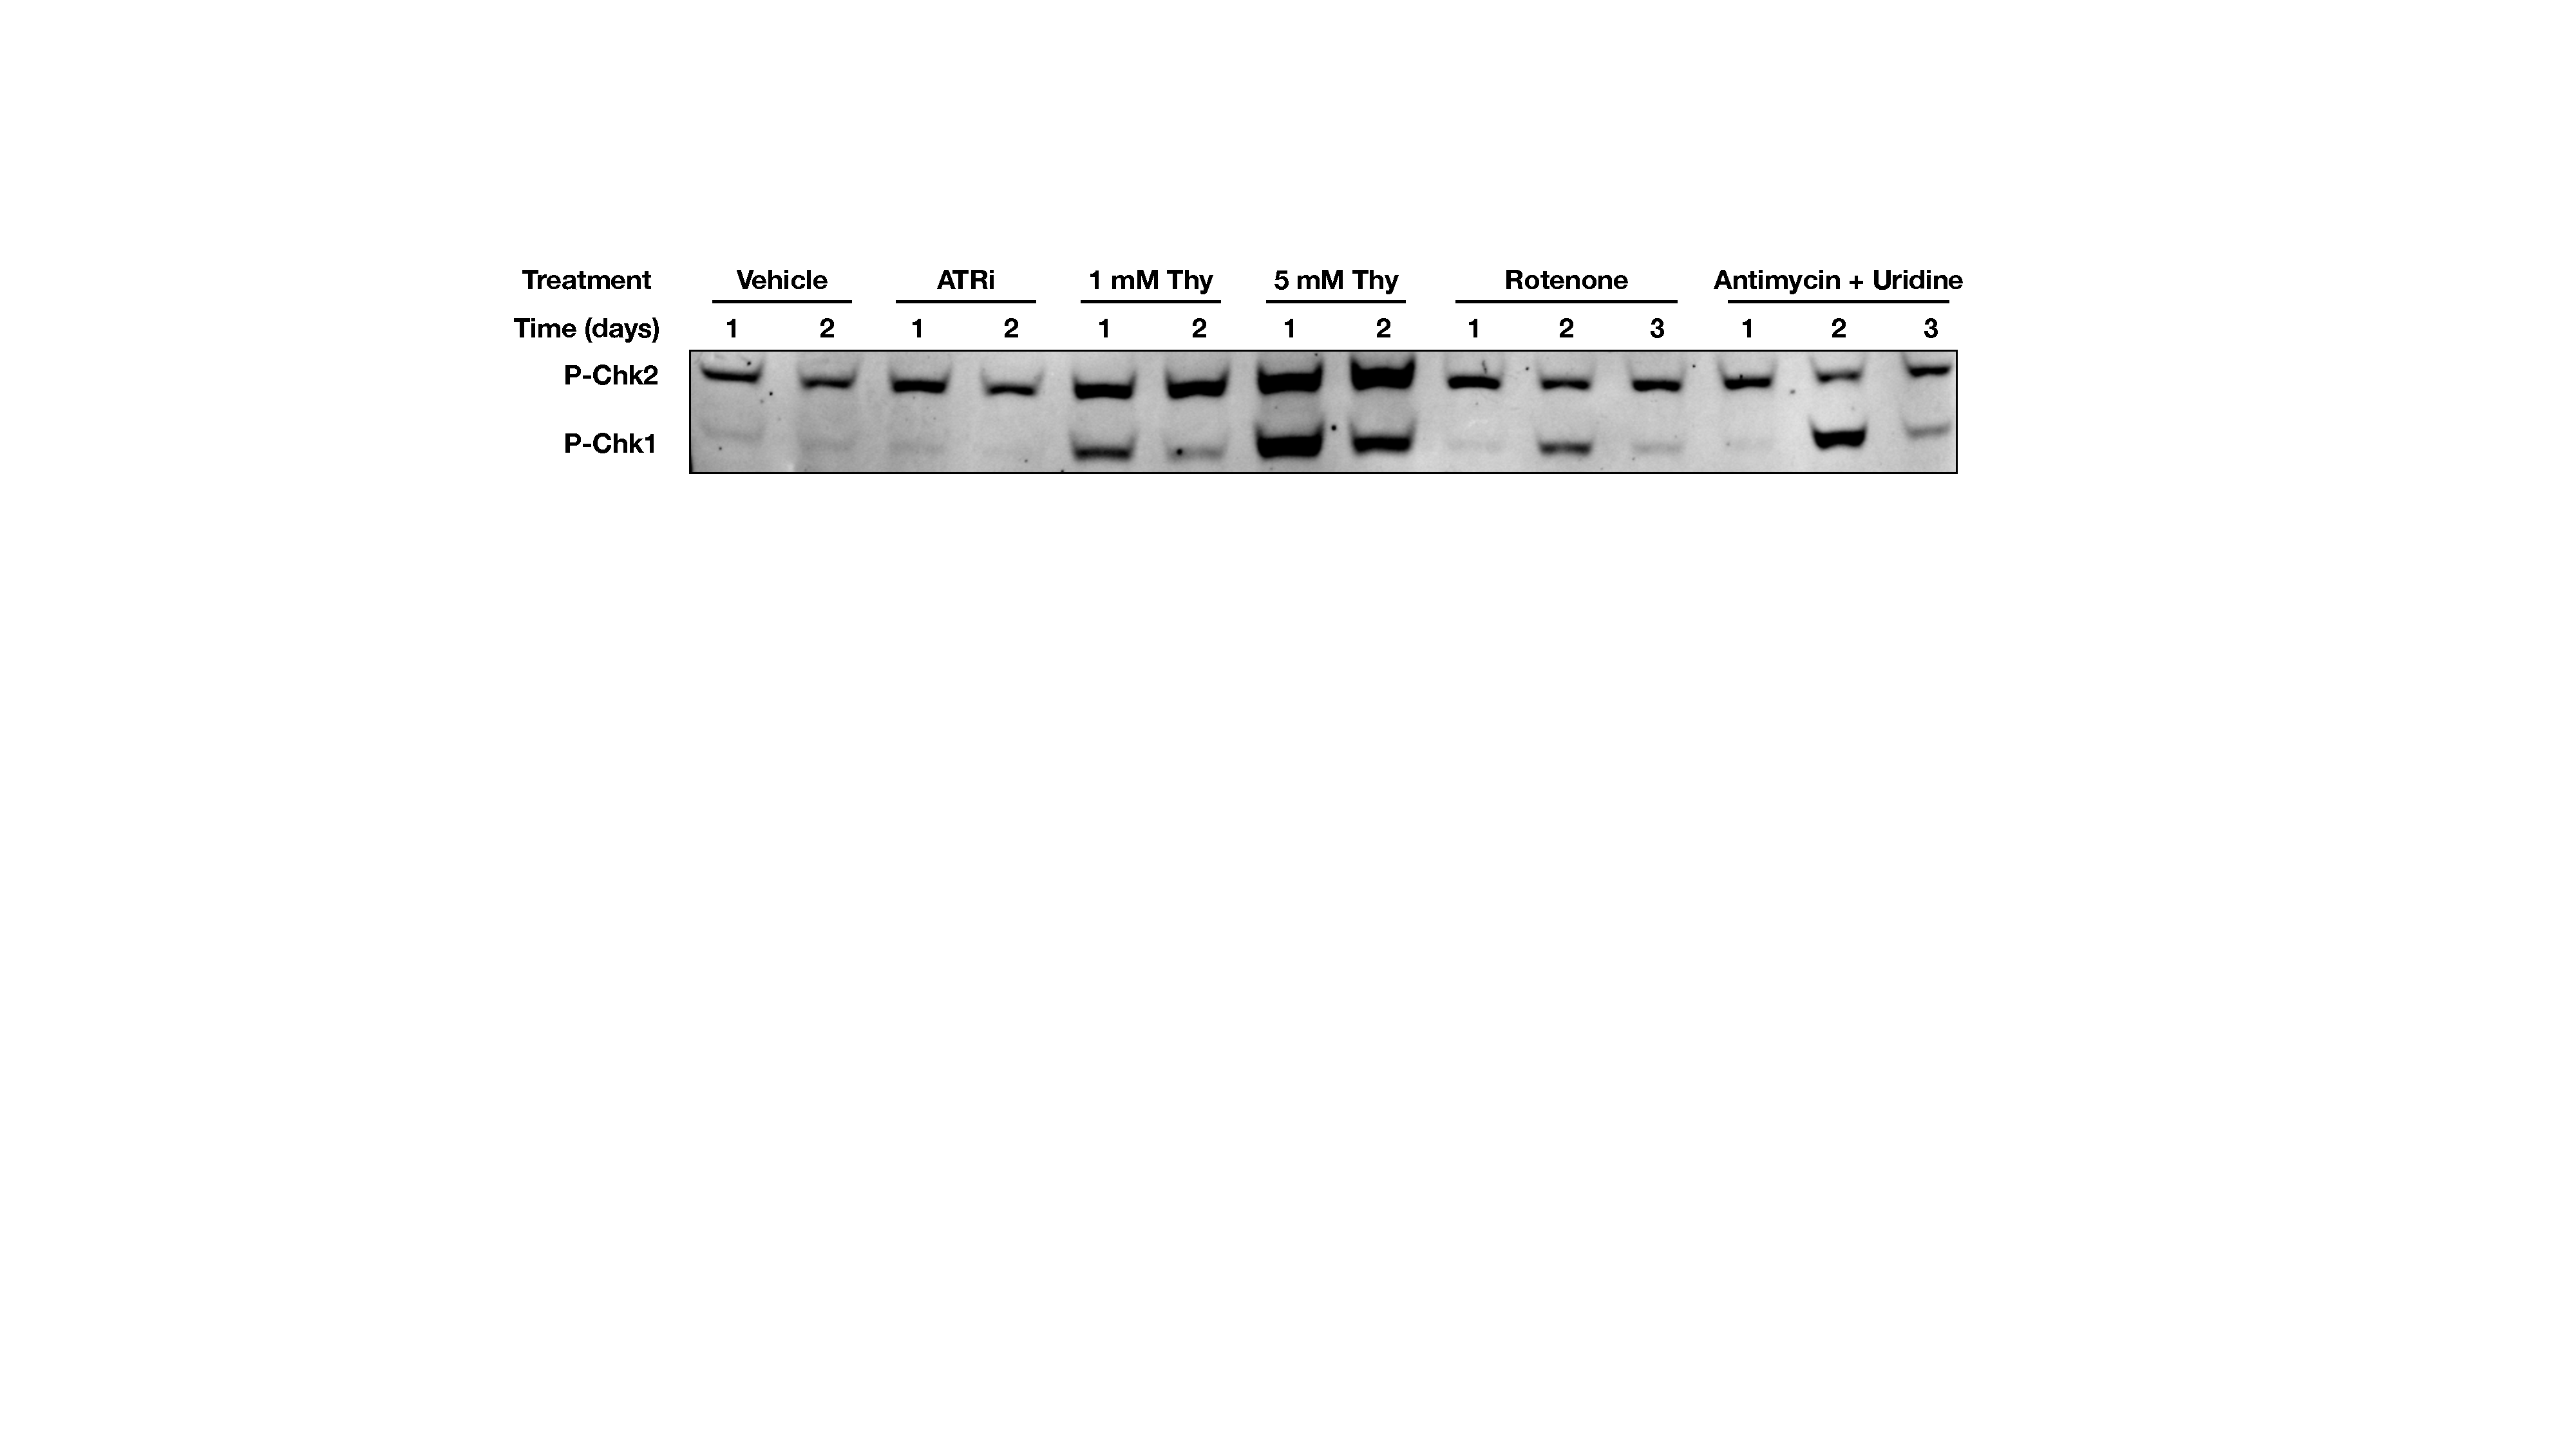
\includegraphics[width=0.85\textwidth]{figures/chap6/P_Chk_wstrn.pdf}
    \caption[gggg]{
    gggg
    }
    \label{fig:ch6:P_Chk_wstrn}
\end{figure}










% Cell signal	2348T	Phospho-Chk1 (Ser345) (133D3) Rabbit mAb #2348
% Cell signal	2197T	Phospho-Chk2 (Thr68) (C13C1) Rabbit mAb #2197
















 \chapter {Introduction}
 
The utility of a clean, professionally prepared thesis is well
documented%
\footnote{See, for example,
  W.~Shakespeare\cite{Hamlet} for a recent discussion.}
but, until recently, a degree candidate had no recourse but
to submit his or her thesis to a typist for completion.
Revisions were difficult and time consuming, and even at its best the
resultant thesis still looked typed.
The advent of computerized typesetting has revolutionized
thesis preparation, and \TeX\ in particular brings to the
university student the power and flexibility of an
`industrial-strength' typesetter.
 
 
\TeX\ is a flexible,
complete, and professional typesetting system.
It has been programmed to produce
the same document on all machines, so
a suitable printer can always be found for the final copy
while drafts are made on more conventional and inexpensive printers.
The `suitable' standard is a 300 dot-per-inch laser printer,
which is excellent for thesis production.  Many such laser printers
are available about the campus.
 
\section{The Purpose of This Sample Thesis}
 
This sample is both a demonstration of the quality and
propriety of a \LaTeX\footnote{We mean the \LaTeXe\ version
of \LaTeX.  Earlier versions, now called \LaTeX2.10 were much
different.} formatted thesis, and is 
documentation for the preparation of a thesis.
It has made extensive use of a custom class file
developed specifically for this purpose
at the University of Washington.  Chapter~II discusses
\TeX\ and \LaTeX.
Chapter III describes the additional macros and functions
provided by the custom thesis class file.  Finally, Chapter IV discusses
some special problems due to the inherent differences among the various
computers and printers that support \LaTeX.
 
It is 
impossible to predict all the formatting problems one will encounter
and there will be problems that are best handled
by a specialist.  
The Graduate School may be able to help you find help.
Some departments may also be able to provide \LaTeX\ assistance.
 
 
\section{Conventions and Notations}
 
In this thesis the typist
refers to the user of \LaTeX---the one who
makes formatting decisions and chooses the appropriate
formatting commands.
He or she will most often be the degree candidate.
 
This document deals with \LaTeX\ typesetting commands and their
functions.  Wherever possible the conventions used to display
text entered by the typist and the resulting formatted output
are the same as those used by the \TeX books.
Therefore, {\tt typewriter type} is used to indicate text
as typed by the computer
or entered by the typist.
It is quite the opposite of {\it italics,} which indicates
a category rather than exact text.  For example,
{\tt alpha} and {\tt beta} might each be an example of a {\it label}.
 
 
\section{Nota bene}
 
This sample thesis was produced by the \LaTeX\ document class it describes
and its format is consonant with the Graduate School's electronic dissertation guidelines%
\cite{SP}.
However, use of this package does not guarantee acceptability
of a particular thesis.
 

% ========== Chapter 2
 
\chapter{A Brief \\ Description of \protect\TeX}
 
The \TeX\ formatting program is the creation of
Donald Knuth of Stanford University.
It has been implemented on nearly every general purpose computer and
produces exactly\footnote{``Exactly'' specifically excludes the
  inherent variety in print devices.}
the same copy on all machines.
 
\section{What is it; why is it spelled that way; 
and what do
really long section titles look like in the text and in the
Table of Contents?}
 
\TeX\ is a formatter.  A document's format is controlled
by commands embedded in the text.
% The peculiar look to the names indicate that \TeX\ is also
% a typesetting program.  Each character and rule on the page
% is precisely positioned.
\LaTeX\ is a special version of \TeX---preloaded
with a voluminous set of macros that simplify most
formatting tasks.
 
\TeX\ uses {\it control sequences} to control
the formatting of a document.  These control sequences are usually
words or groups of letters prefaced with the backslash character
({\tt\char'134}).
For example,
Figure \ref{start-2} shows the text that printed the beginning
of this chapter.  Note the control sequence \verb"\chapter" that
instructed \TeX\ to start a new chapter, print the title, and
make an entry in the table of contents.  It is an example
of a macro defined by the \LaTeX\ macro package.
The control sequence \verb"\TeX", which prints the word \TeX,
is a standard macro from the {\it\TeX book}.
The short control sequence \verb"\\" in the title instructed \TeX\ to
break the title line at that point.
This capability is an example of an extension to \LaTeX\
provided by the uwthesis document class.
 
\begin{figure}
\begin{demo}
\\chapter\{A Brief\\\\Description of \\TeX\}

The \\TeX\\ formatting program is the creation of
Donald Knuth of Stanford University.
\end{demo}
\label{start-2}
\caption{The beginning of the Chapter II text}
\end{figure}
 
Most of the time \TeX\ is simply building paragraphs from
text in your source files.  No control sequences are involved.
New paragraphs are indicated by a blank line in the
input file.
Hyphenation is performed automatically.
 
\section{\TeX books}
 
The primary reference for \LaTeX\ is Lamport's second edition
of the \textit{\LaTeX\ User's Guide}\cite{Lbook}.
It is easily read and should be sufficient for thesis formatting.
See also the \textsl{\LaTeX\ Companion}\cite{companion} for descriptions
of many add-on macro packages.

Although unnecessary for thesis writers, the \textsl{\TeX book}
is the primary reference for \TeX sperts worldwide.
 

 
 
\section{Languages other than English}
 
Most \LaTeX\ implementations at the University are tailored
for the English language.  However, \LaTeX\ will format many
other languages. 
Consult your department or contact the
Center for Advanced Research Technology in the Arts and Humanities (CARTAH),
\smallskip
\begin{center}
{\tt cartha@u.washington.edu},
\end{center}
\smallskip
for assistance with non-English formatting.

Unusual characters can be defined via the
font maker \hbox{\mffont METAFONT} (documented by Knuth\cite{Metafont}).
The definitions are not trivial.
Students who attempt to print a thesis with
custom fonts may soon proclaim,
 
% note.  This is not the correct way to print Greek
\medskip
\begin{center}
``$\mathaccent"7027\alpha\pi o\kern1pt\theta\alpha\nu\epsilon\hat\iota\nu$
\ $\theta\acute\epsilon\lambda\omega$.''
 
\end{center}
 
% ========== Chapter 3
 
\chapter{The Thesis Unformatted}
 
This chapter describes the uwthesis class (\texttt{uwthesis.cls},
version dated 2011/06/27)
in detail 
and shows how it was used to format the thesis.
A working knowledge of Lamport's \LaTeX\ manual\cite{Lbook} is assumed.
 
\section{The Control File}
 
The source to this sample thesis is contained in a single file
only because ease of distribution was a concern.
You should not do this.  Your task will be much easier if you
break your thesis into several files:  a file for the preliminary pages,
a file for each chapter,  one for the glossary, and one for each
appendix.  Then use a control file to tie them all together.
This way you can edit and format parts of your thesis much more
efficiently.
 
Figure~\ref{control-file} shows a control file that
might have produced this thesis.
It sets the document style, with options and parameters,
and formats the various parts of the thesis---%
but contains no text of its own.
 
 
%  control file caption and figure
%
\begin{figure}[p]
 \begin{leftfullpage}
  \caption[A thesis control file]%
   {\narrower A thesis control file ({\tt thesis.tex}).
   This file is the input to \LaTeX\ that will produce a
   thesis.  It contains no text, only commands which
   direct the formatting of the thesis.
   This is also an example of a `facing page' caption.  It is guaranteed
   to appear on a lefthand page, facing the figure contents on the right.
   See the text.}
  \label{control-file}
 \end{leftfullpage}
\end{figure}
%
\begin{figure}[p]
%
 \begin{fullpage}
  \footnotesize
  \begin{verbatim}
    % LaTeX thesis control file
 
    \documentclass[11pt,twoside]{uwthesis}
 
    \begin{document}
 
    % preliminary pages
    %
    \prelimpages
    \include{prelim}
 
    % text pages
    %
    \textpages
    \chapter{Aspartate in cellular metabolism}
blaa

\section{Introduction}
More blaa

\subsection{Intro subject 1}
qwerty

\subsection{Intro subject 2}
qwerty
\subsection{Details}
qwerty1


\begin{figure}
    \centering
    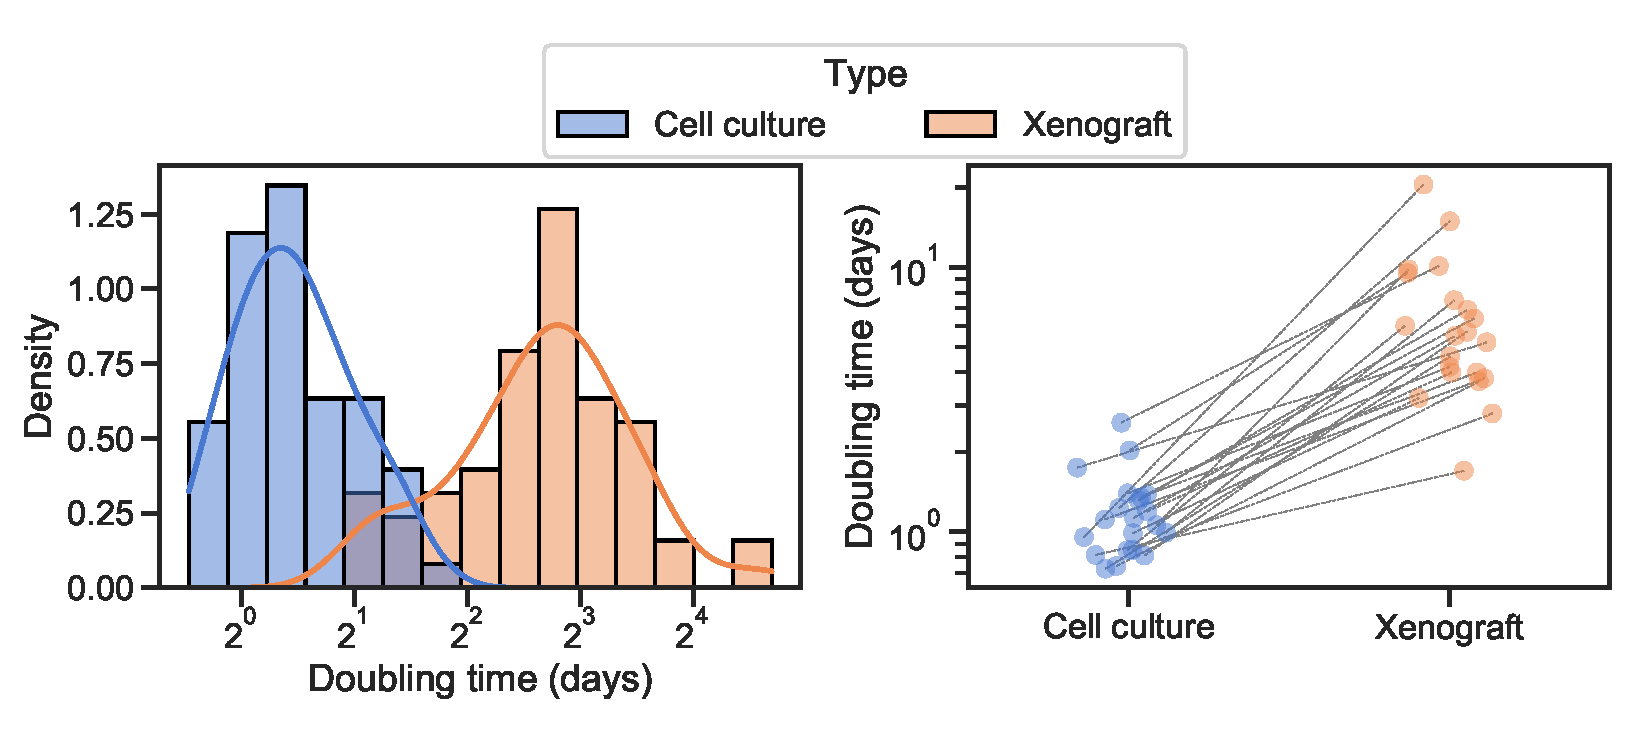
\includegraphics[width=0.70\textwidth]{figures/chap1/prlfr_contr.pdf}
    \caption[gggg]{
    gggg
    }
    \label{fig:ch1:prlfr_contr}
\end{figure}











\begin{figure}
    \centering
    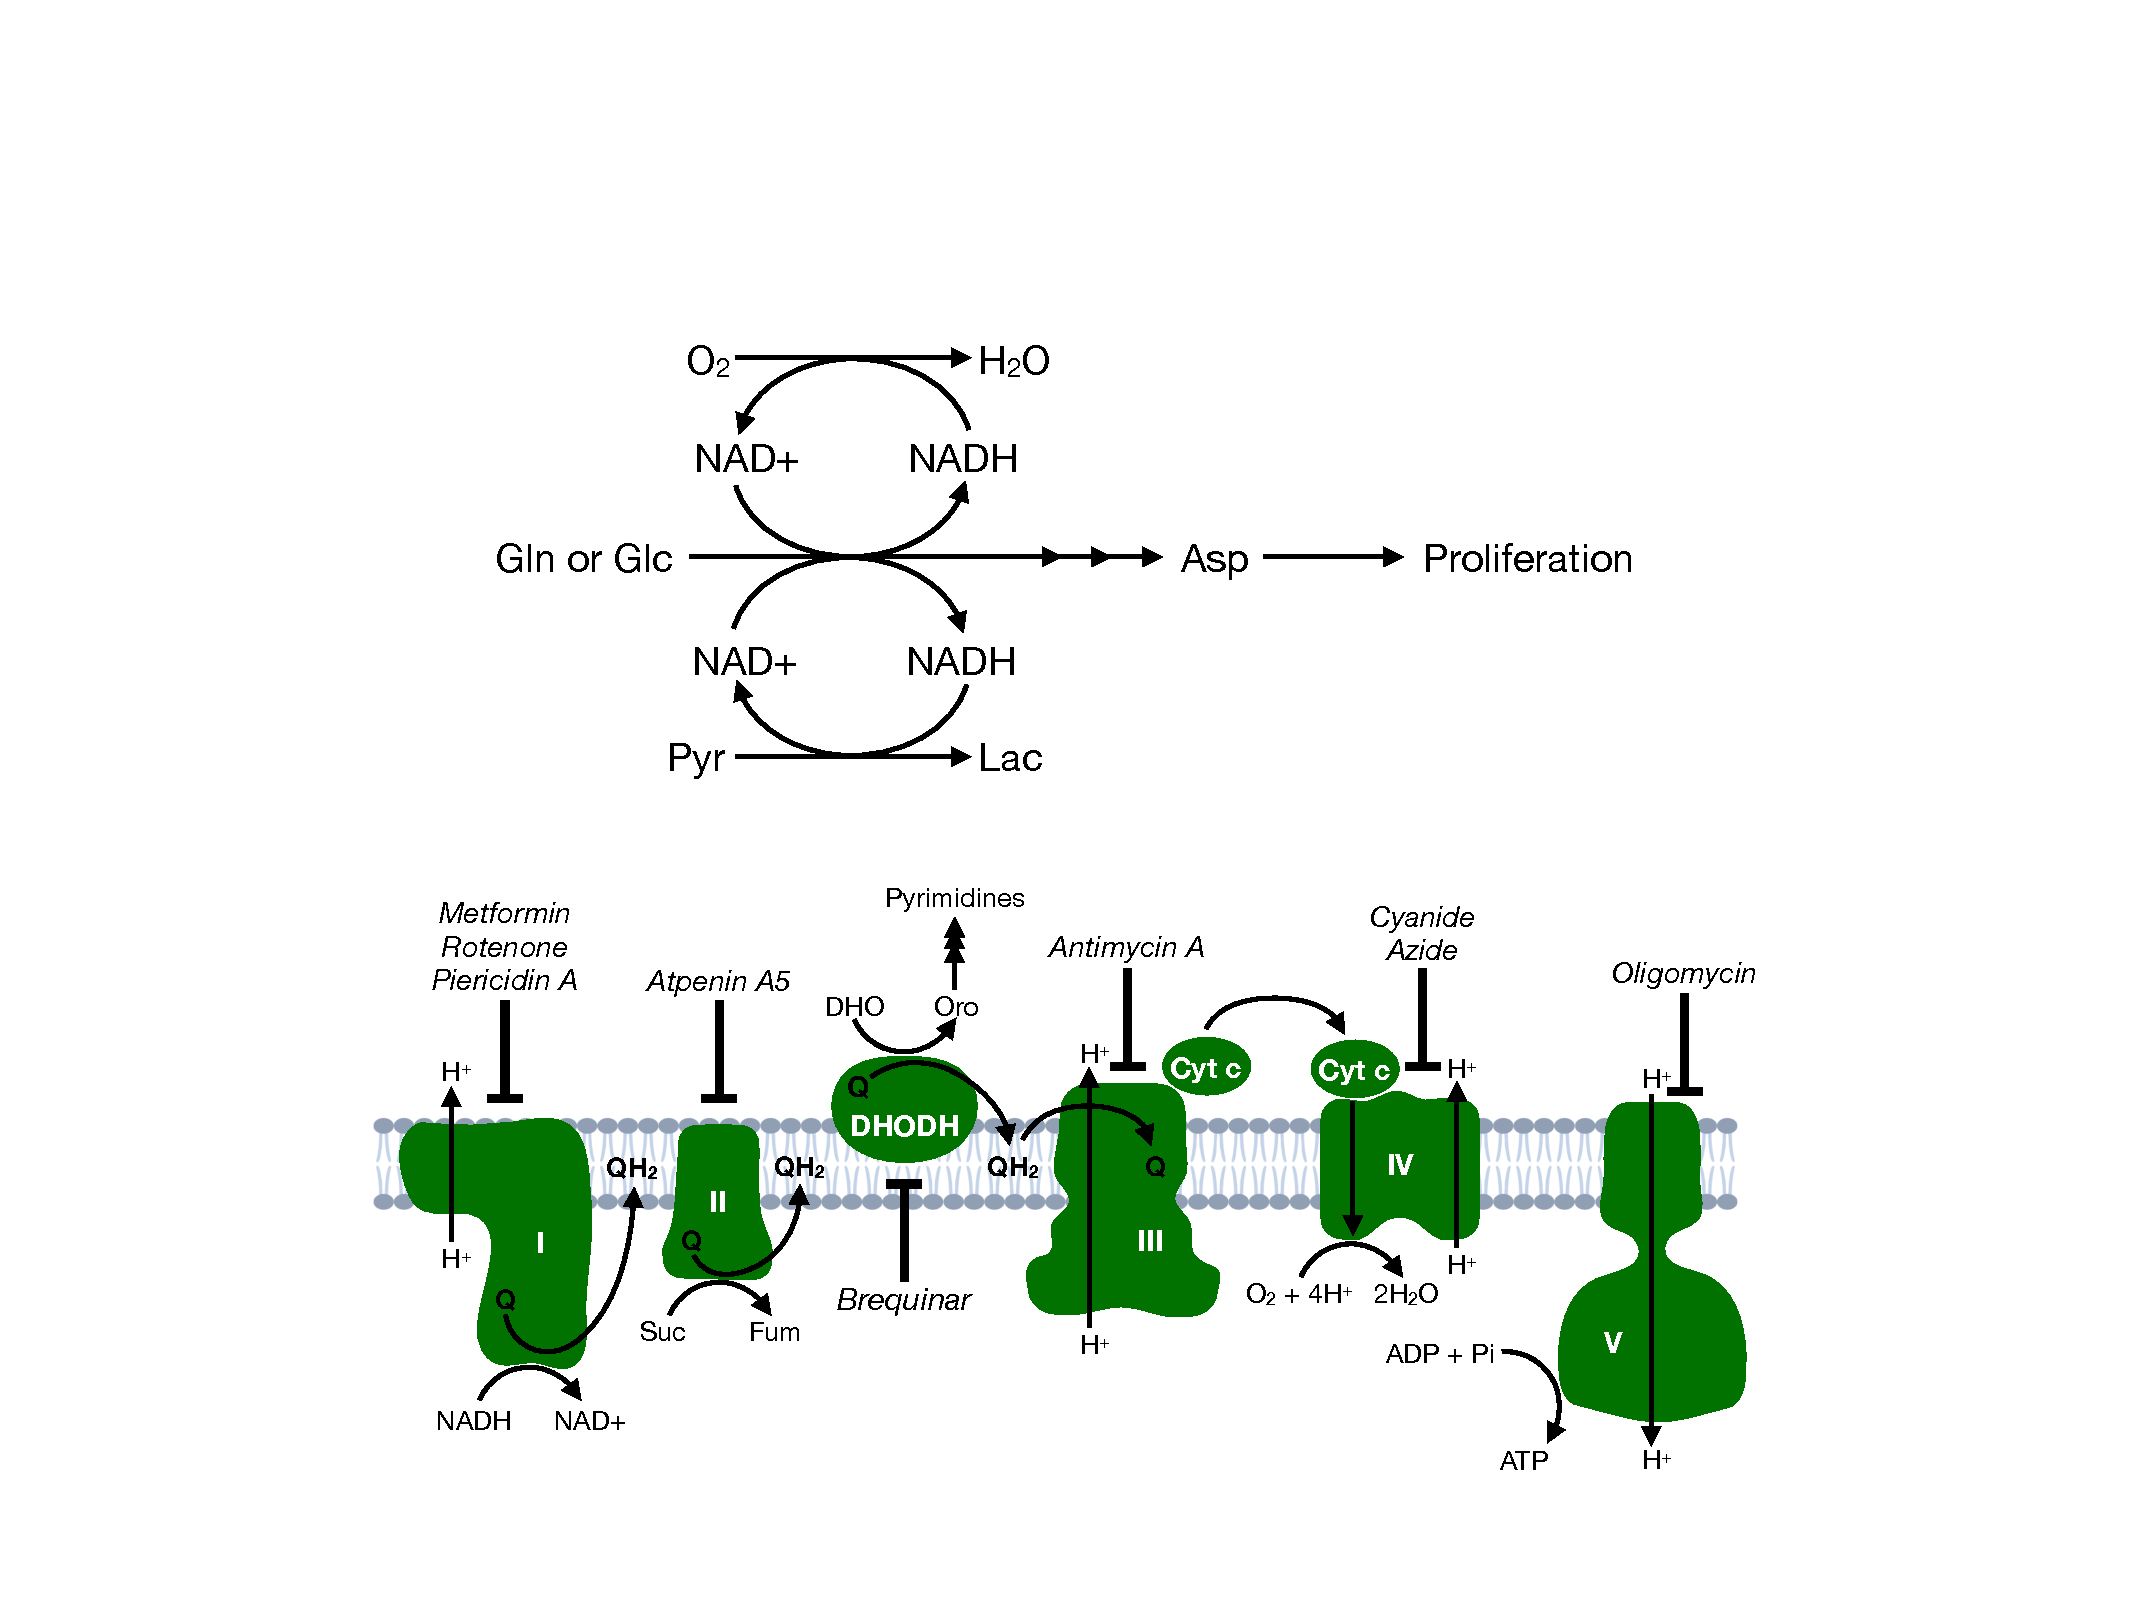
\includegraphics[width=0.70\textwidth]{figures/chap1/redox_biomass.pdf}
    \caption[Biomass accumulation requires NAD+ regeneration]{
    gggg
    }
    \label{fig:ch1:redox_biomass}
\end{figure}







Aspartate is typically coupled to NAD+/NADH ratio and thus if one is changed the other one is changed proportionally an vice versa.
Therefore it could be compelling to think that aspartate levels correlate with proliferation only indirectly through the NAD+/NADH ratio.
However, we have evidence against this:
Lucas' previous papers
My NAD+/NADH experiment with 143B SLC1A3 cells
Maddie's paper on SHDB which shows the opposite trend i.e. increased cytoplasmic NAD+/NADH ratio (due to media pyruvate) but are still aspartate limited



\begin{figure}
    \centering
    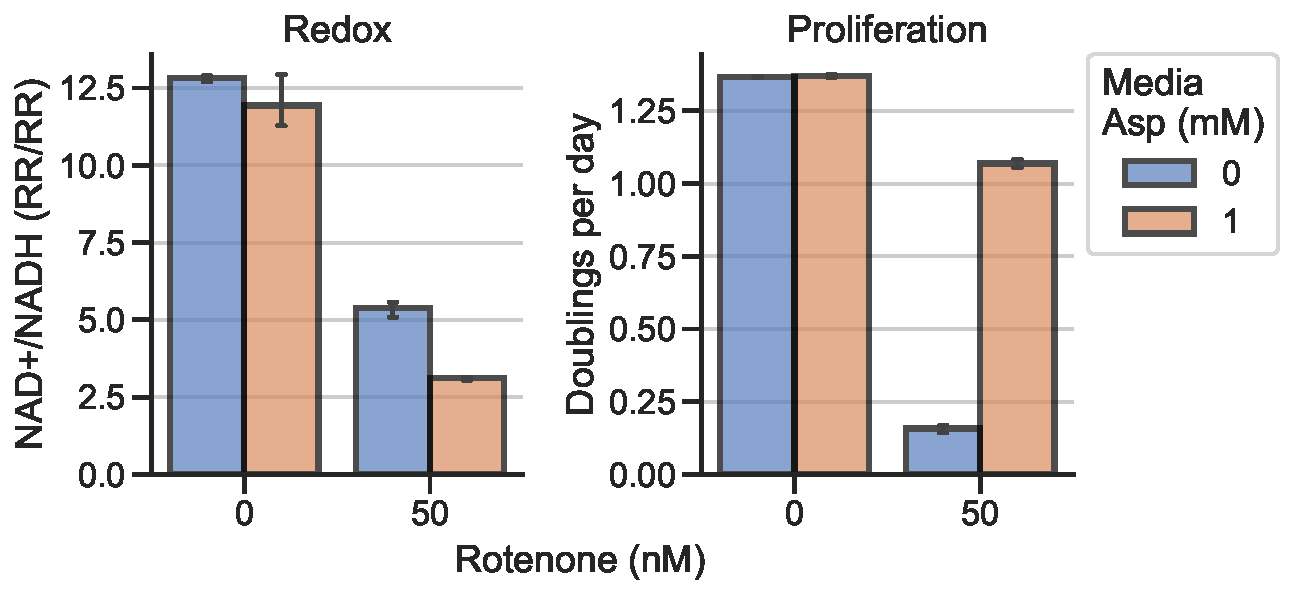
\includegraphics[width=0.70\textwidth]{figures/chap1/redox-prlfr_uncpl.pdf}
    \caption[Aspartate rescues proliferation but not the NAD+/NADH ratio]{
    Aspartate rescues proliferation but not the NAD+/NADH ratio.
    Uncoupling NAD+/NADH and aspartate's effect on proliferation using 143B cells with stable expression of the Glu/Asp transporter SLC1A3, treated with/without 1 mM media aspartate and with/without 50 nM rotenone.
    NAD+/NADH ratio measured using LCMS as a ratio between two internal standard normalized response ratios (RR/RR).
    }
    \label{fig:ch1:redox-prlfr_uncpl}
\end{figure}







\begin{figure}
    \centering
    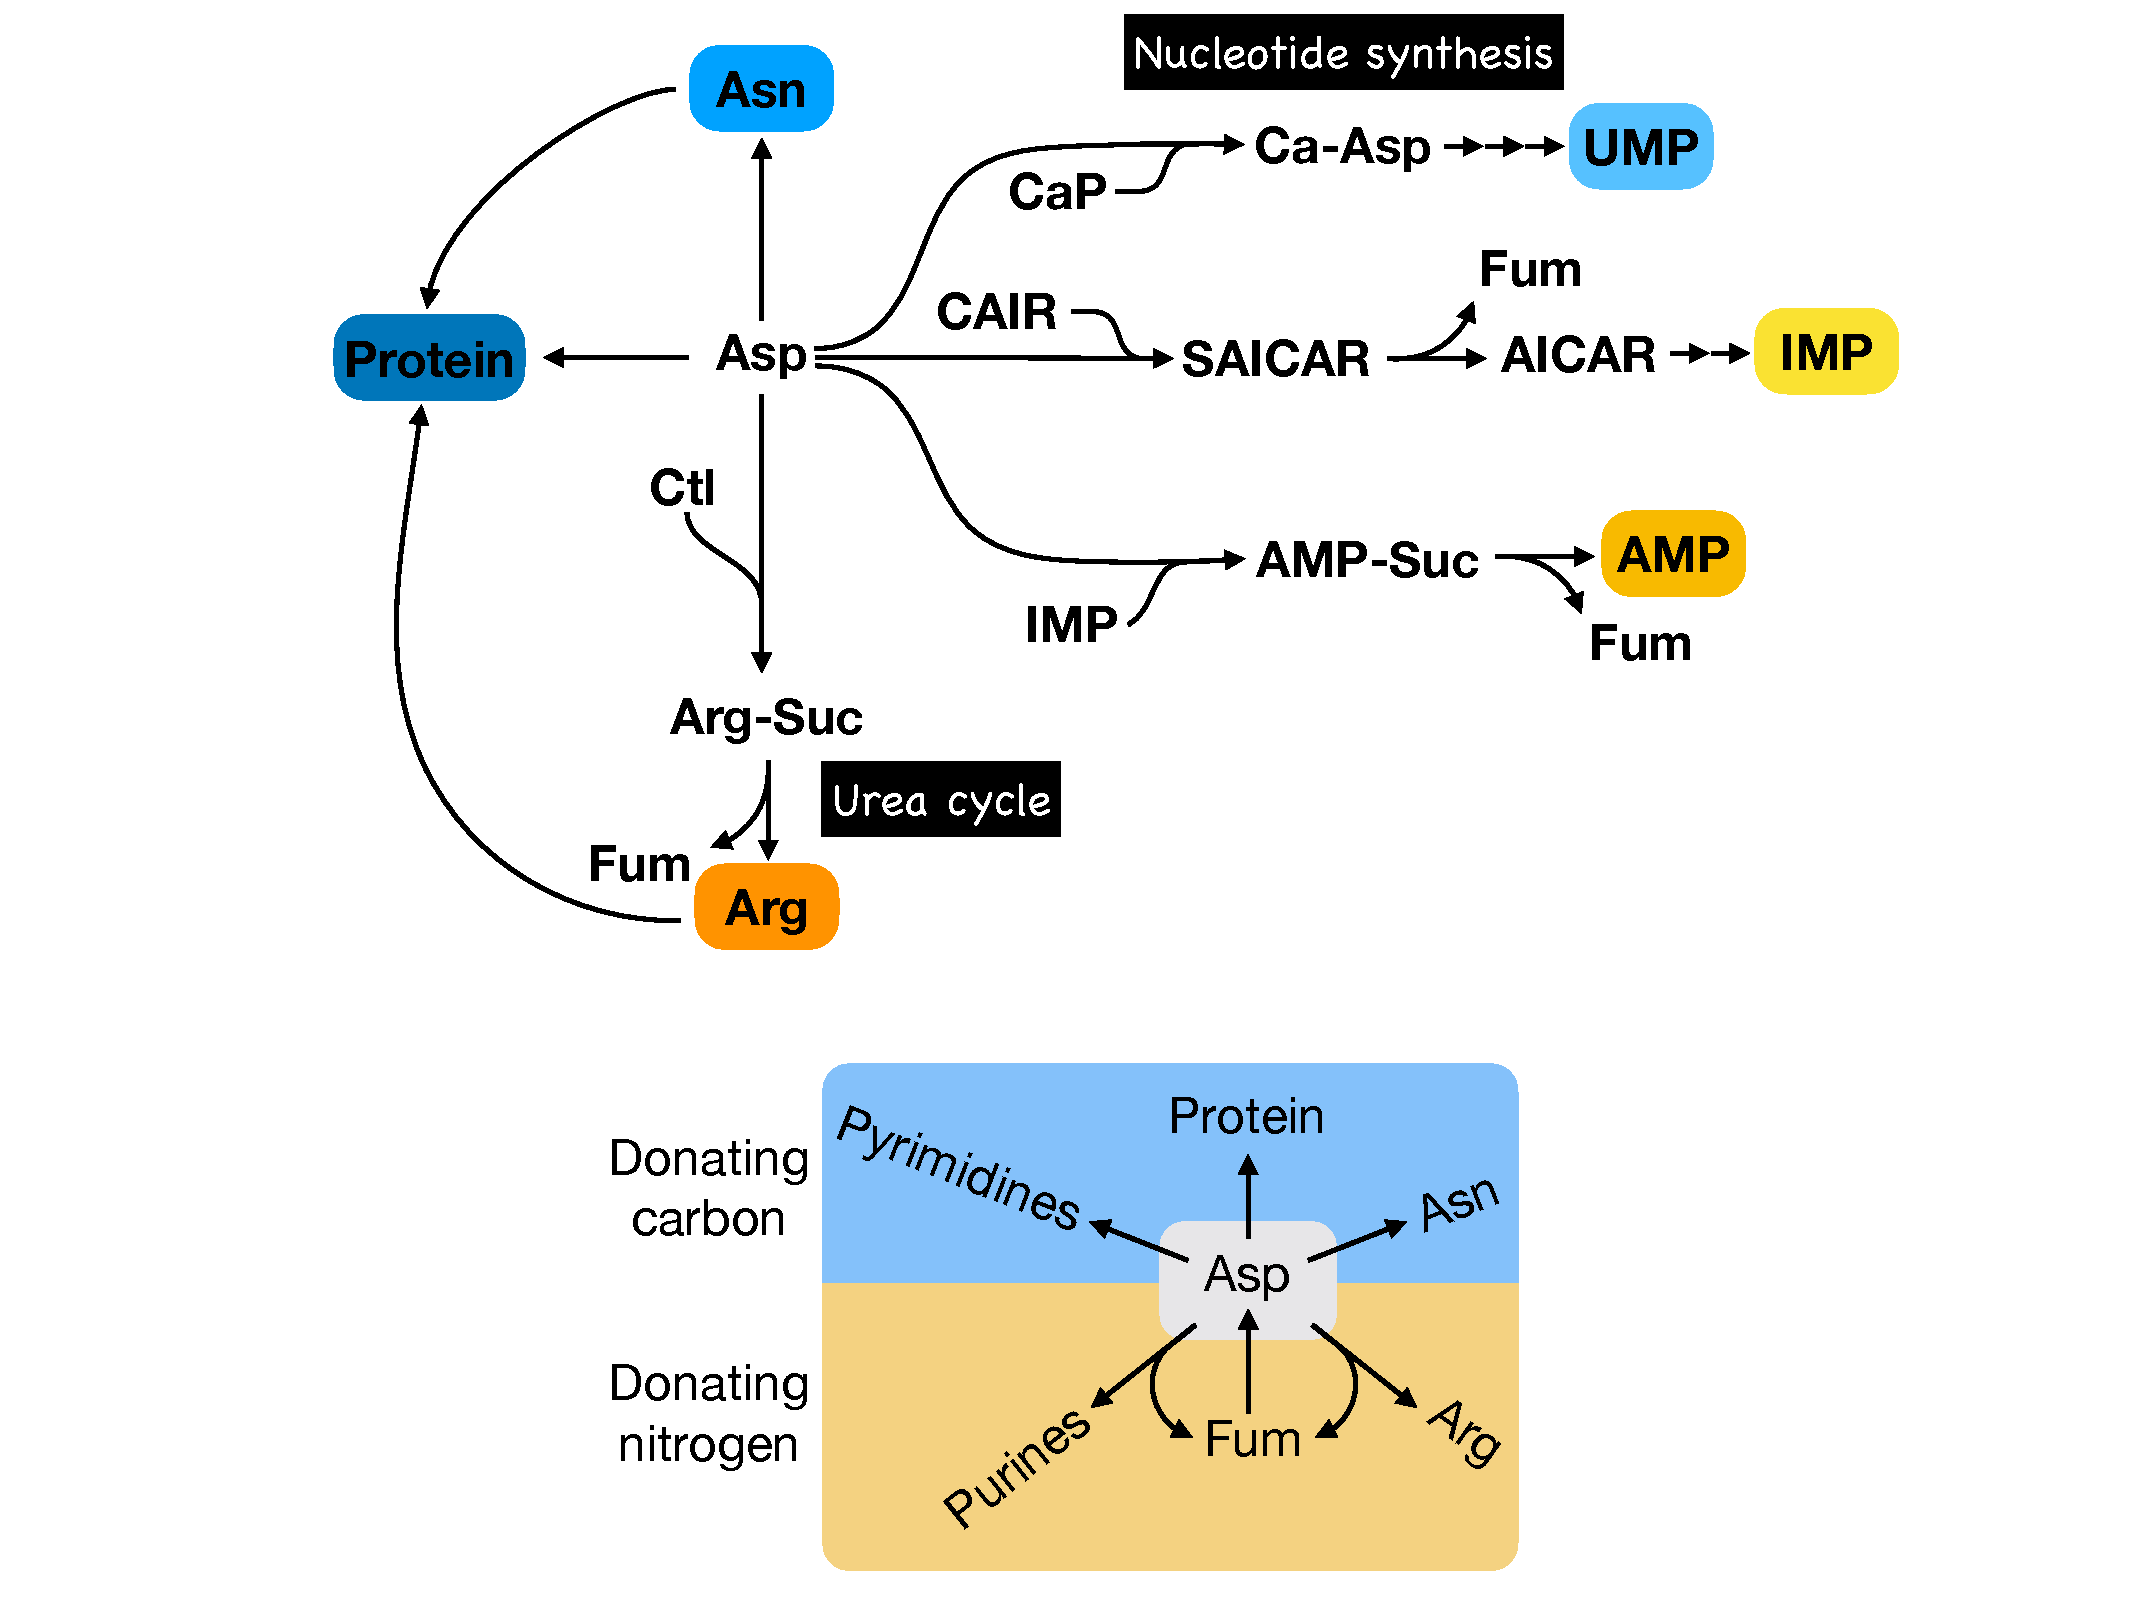
\includegraphics[width=0.70\textwidth]{figures/chap1/asp_fates.pdf}
    \caption[Metabolic fates of aspartate]{
    gggg
    }
    \label{fig:ch1:asp_fates}
\end{figure}




\begin{figure}
    \centering
    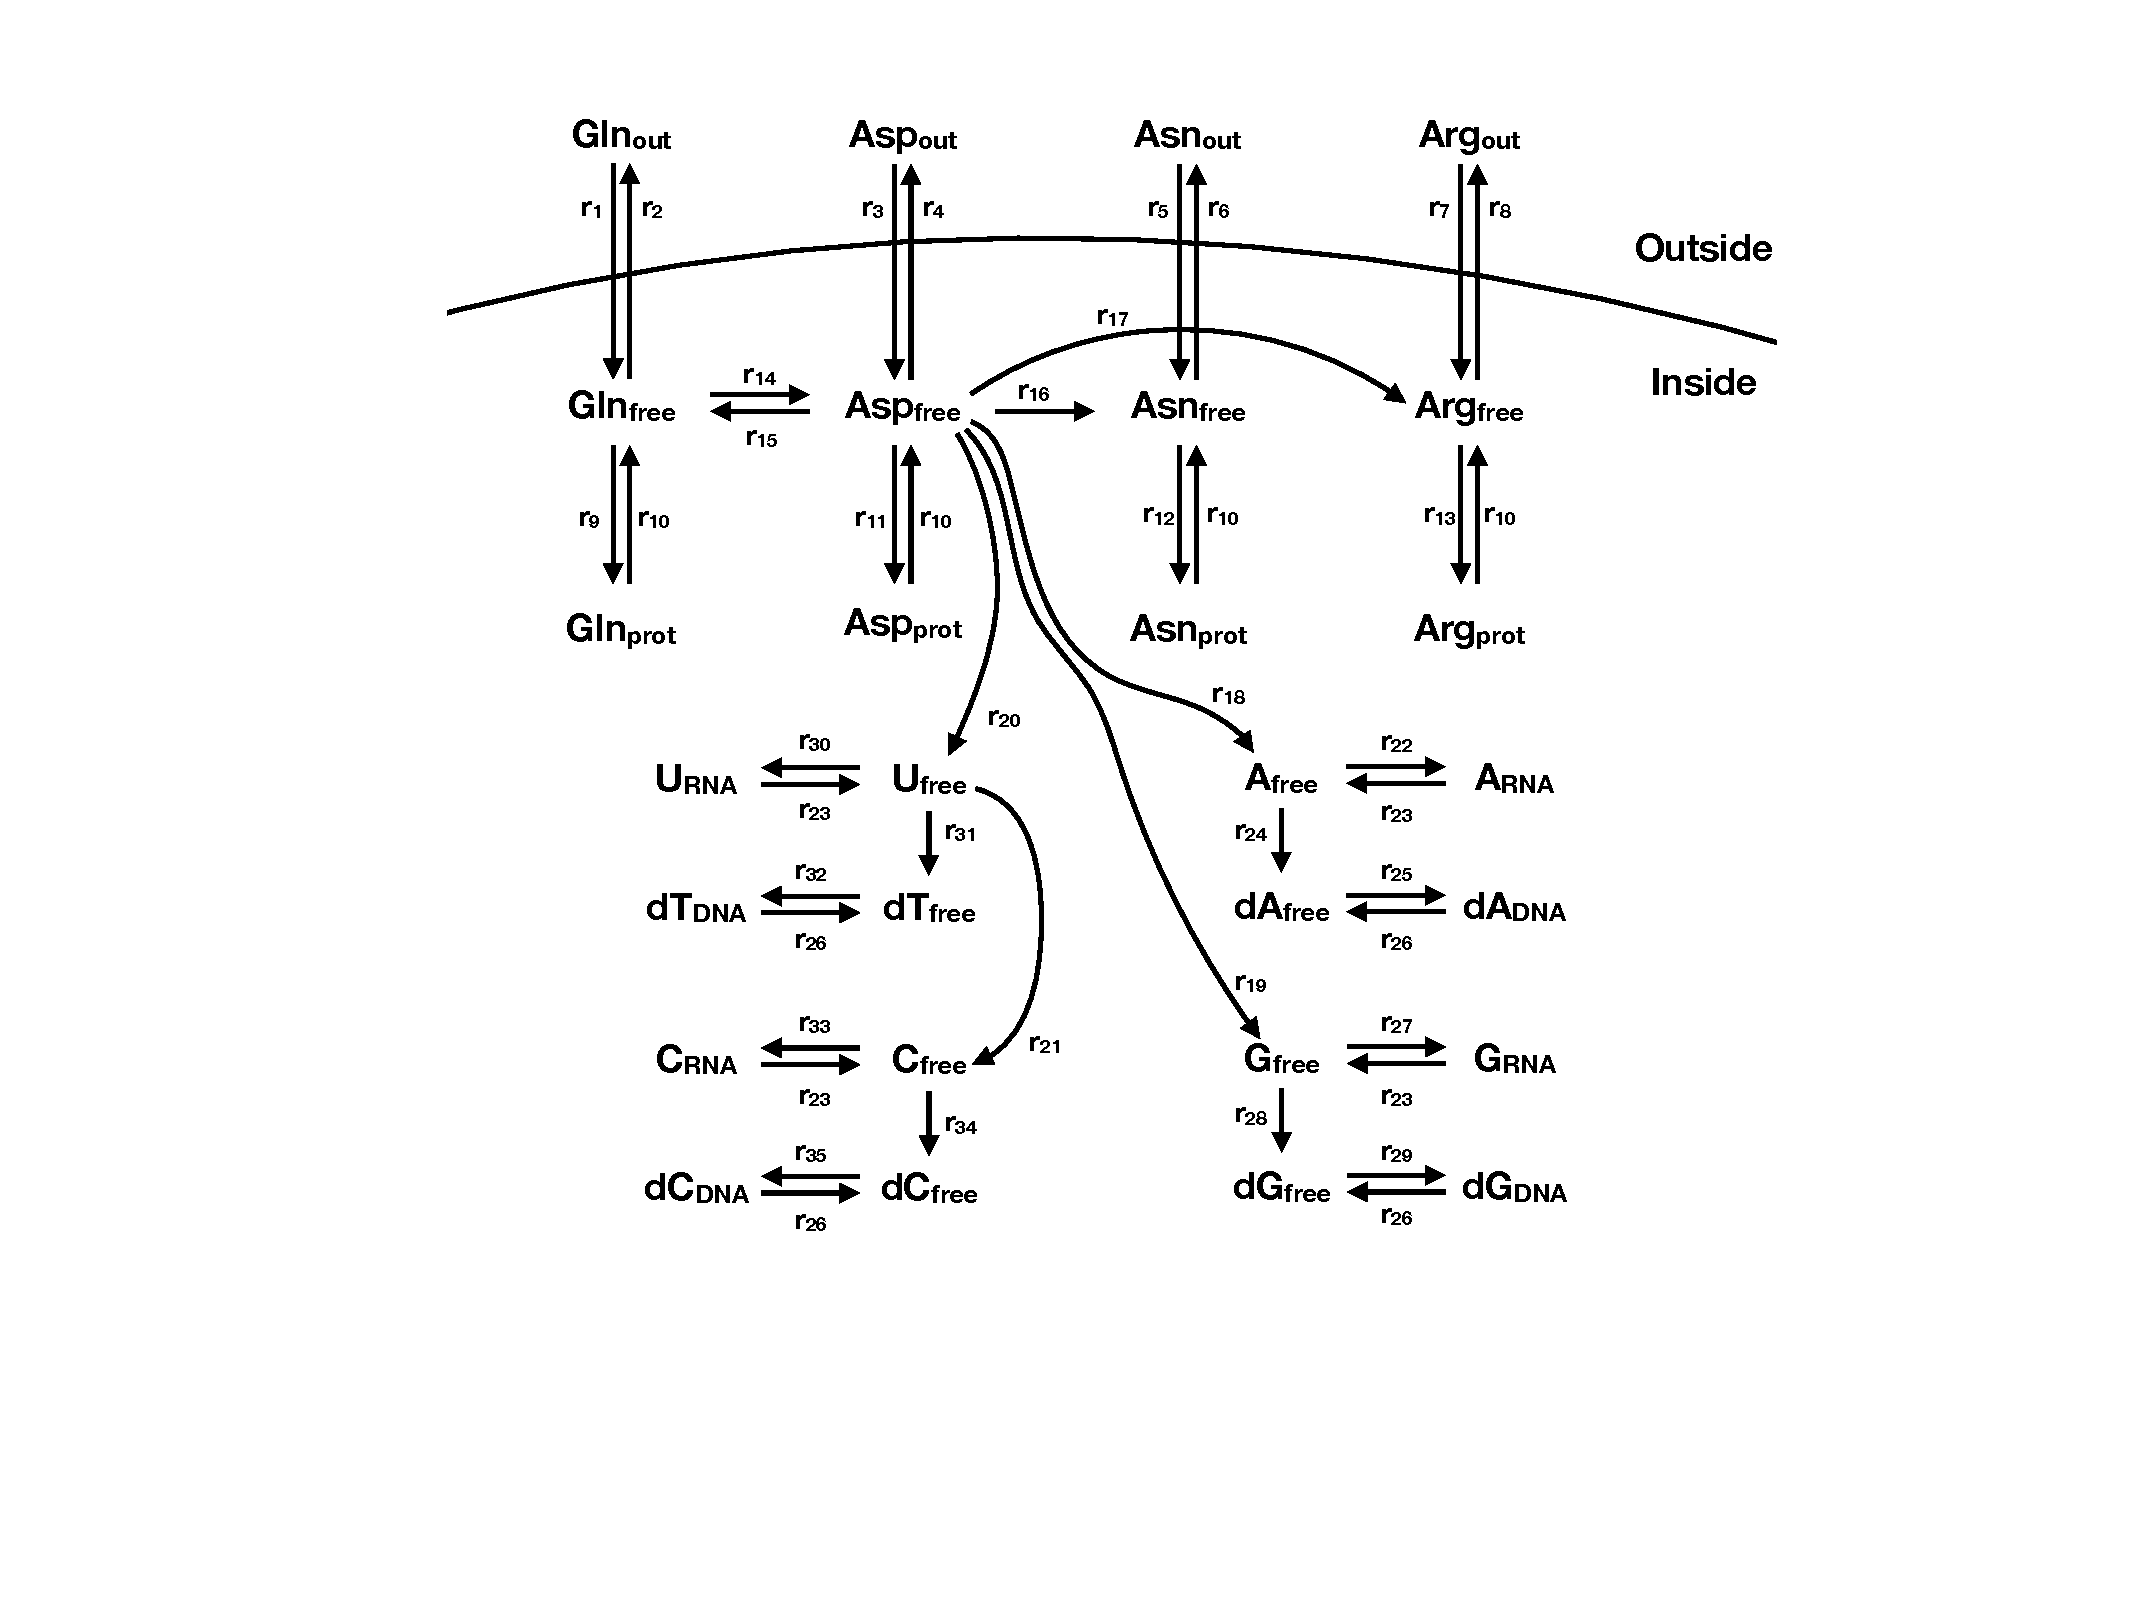
\includegraphics[width=0.70\textwidth]{figures/chap1/asp_fluxes.pdf}
    \caption[Aspartate metabolism fluxes]{
    gggg
    }
    \label{fig:ch1:asp_fluxes}
\end{figure}



\begin{figure}
    \centering
    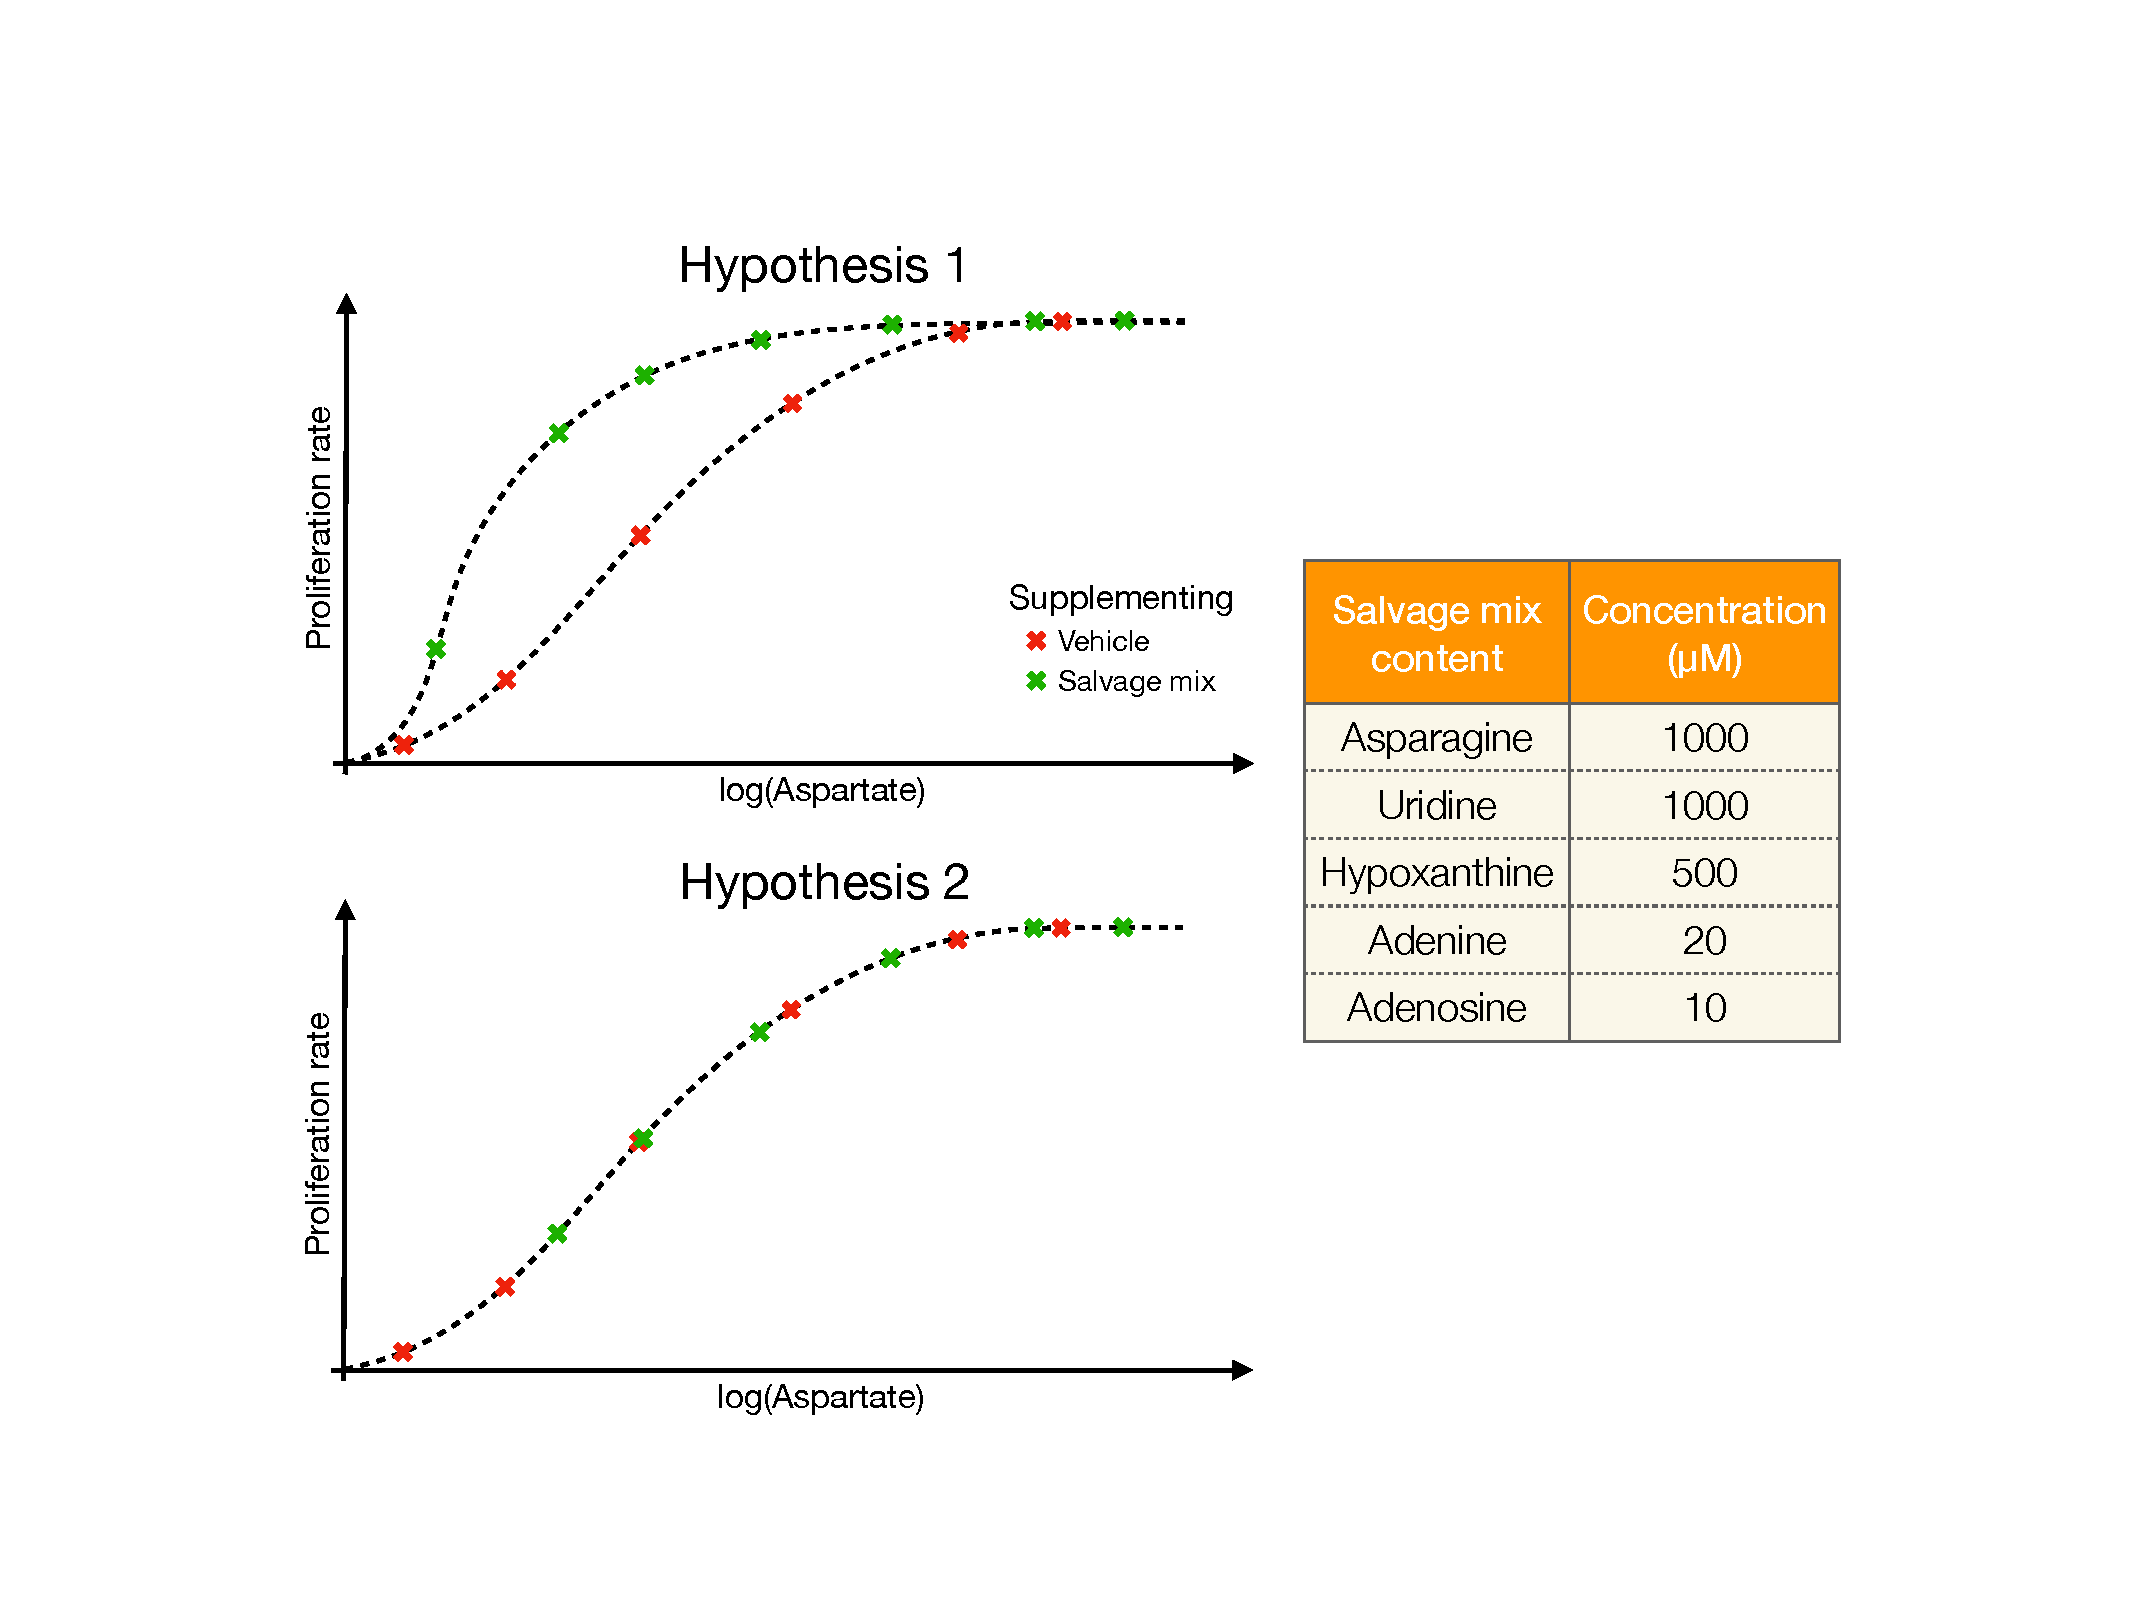
\includegraphics[width=0.70\textwidth]{figures/chap1/asp_fates_suppl_hypo.pdf}
    \caption[Two hypotheses for aspartate to proliferation correlation]{
    gggg
    }
    \label{fig:ch1:asp_fates_suppl_hypo}
\end{figure}










    \chapter{Molecular mechanisms of aspartate limitation}
blaa

\section{Introduction}
More blaa




\section{Mitochondrial inhibition induces a stable relationship between aspartate levels and proliferation rate}
%%% Experiments with H1299 and count/metabolites per day
%% Under ETCinhib_timeseries in lab-work







\section{Quantifying the metabolic fates of aspartate}


\begin{figure}
     \centering
     \begin{subfigure}[b]{0.75\textwidth}
         \centering
         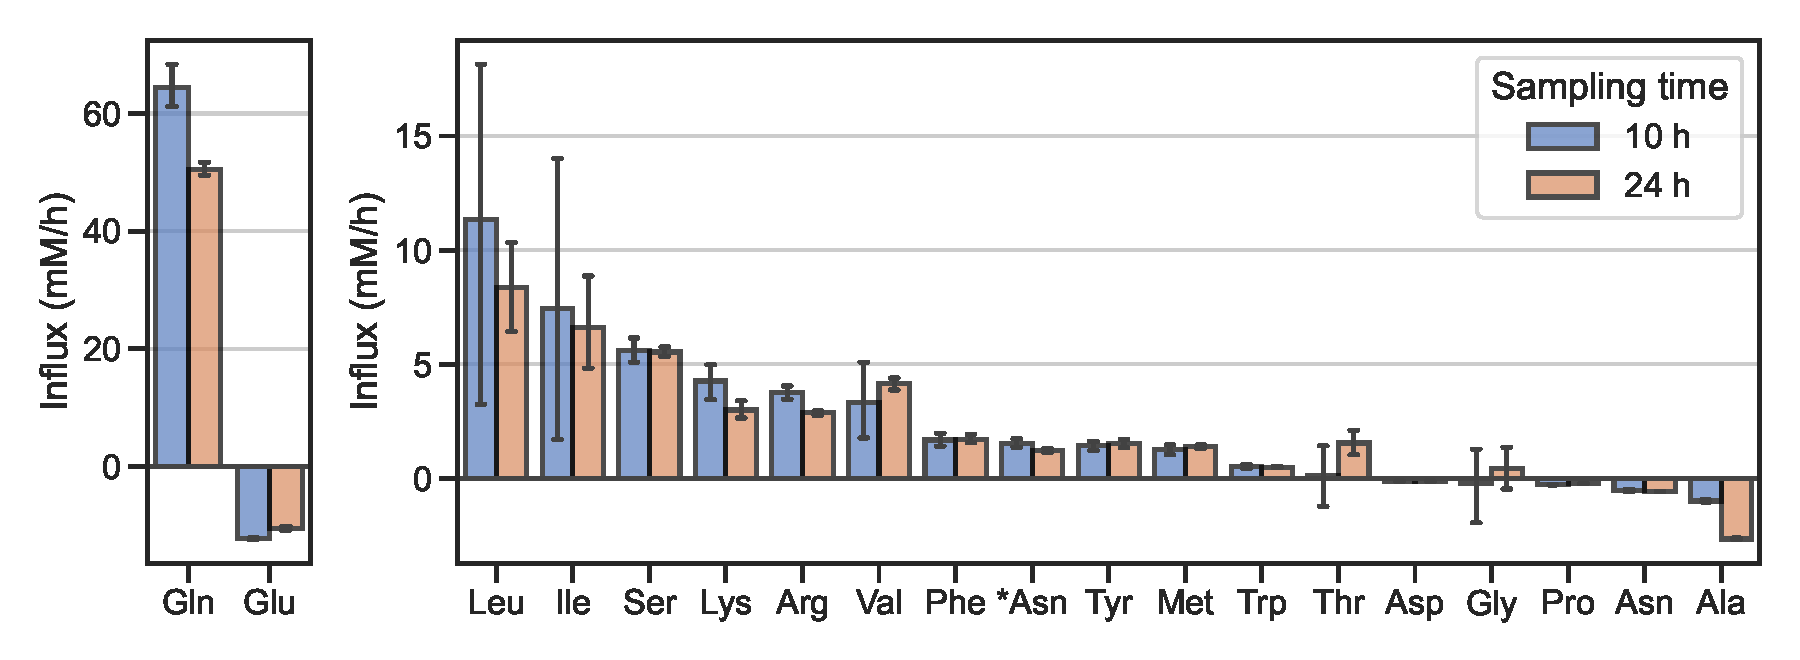
\includegraphics[width=\textwidth]{figures/chap2/flux_143wt.pdf}
         \caption{Media uptake 143B WT}
         \label{fig:ch2:flux_143wt}
     \end{subfigure}
     \begin{subfigure}[b]{0.75\textwidth}
         \centering
         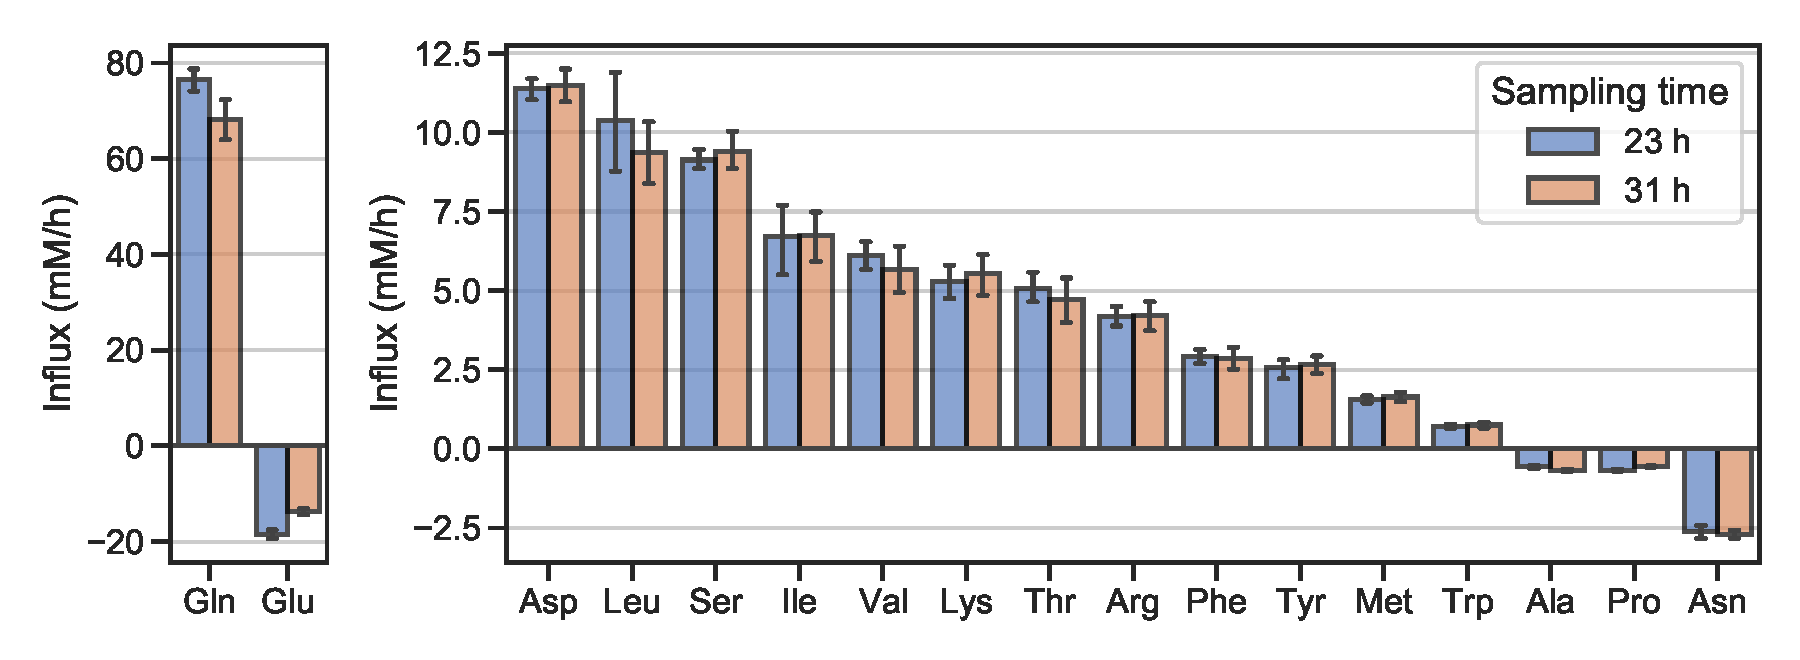
\includegraphics[width=\textwidth]{figures/chap2/flux_143dko.pdf}
         \caption{Media uptake 143B GOT DKO}
         \label{fig:ch2:flux_143dko}
     \end{subfigure}
        \caption[Media amino acid uptake]{
        Amino acid influx/efflux from DMEM.
        For 143B WT in (a), media was spiked with U-\hCi{} Asn (*Asn in the plot) to measure asparagine uptake which, taken together with the labelling fraction, was used to calculate the net asparagine consumption.
        For 143B GOT DKO in (b), cell expressed Glu/Asp transporter SLC1A3 and media was spiked with aspartate to measure its uptake.
        }
\end{figure}



Good correspondence between Asn efflux estimated through labelled Asn in 143B WT (figure \ref{fig:ch2:Asn_flux}) and measured Asn efflux in 143B GOT DKO (figure \ref{fig:ch2:flux_143dko}).
\begin{figure}
     \centering
     \hspace{0.05\textwidth}
     \begin{subfigure}[b]{0.35\textwidth}
         \centering
         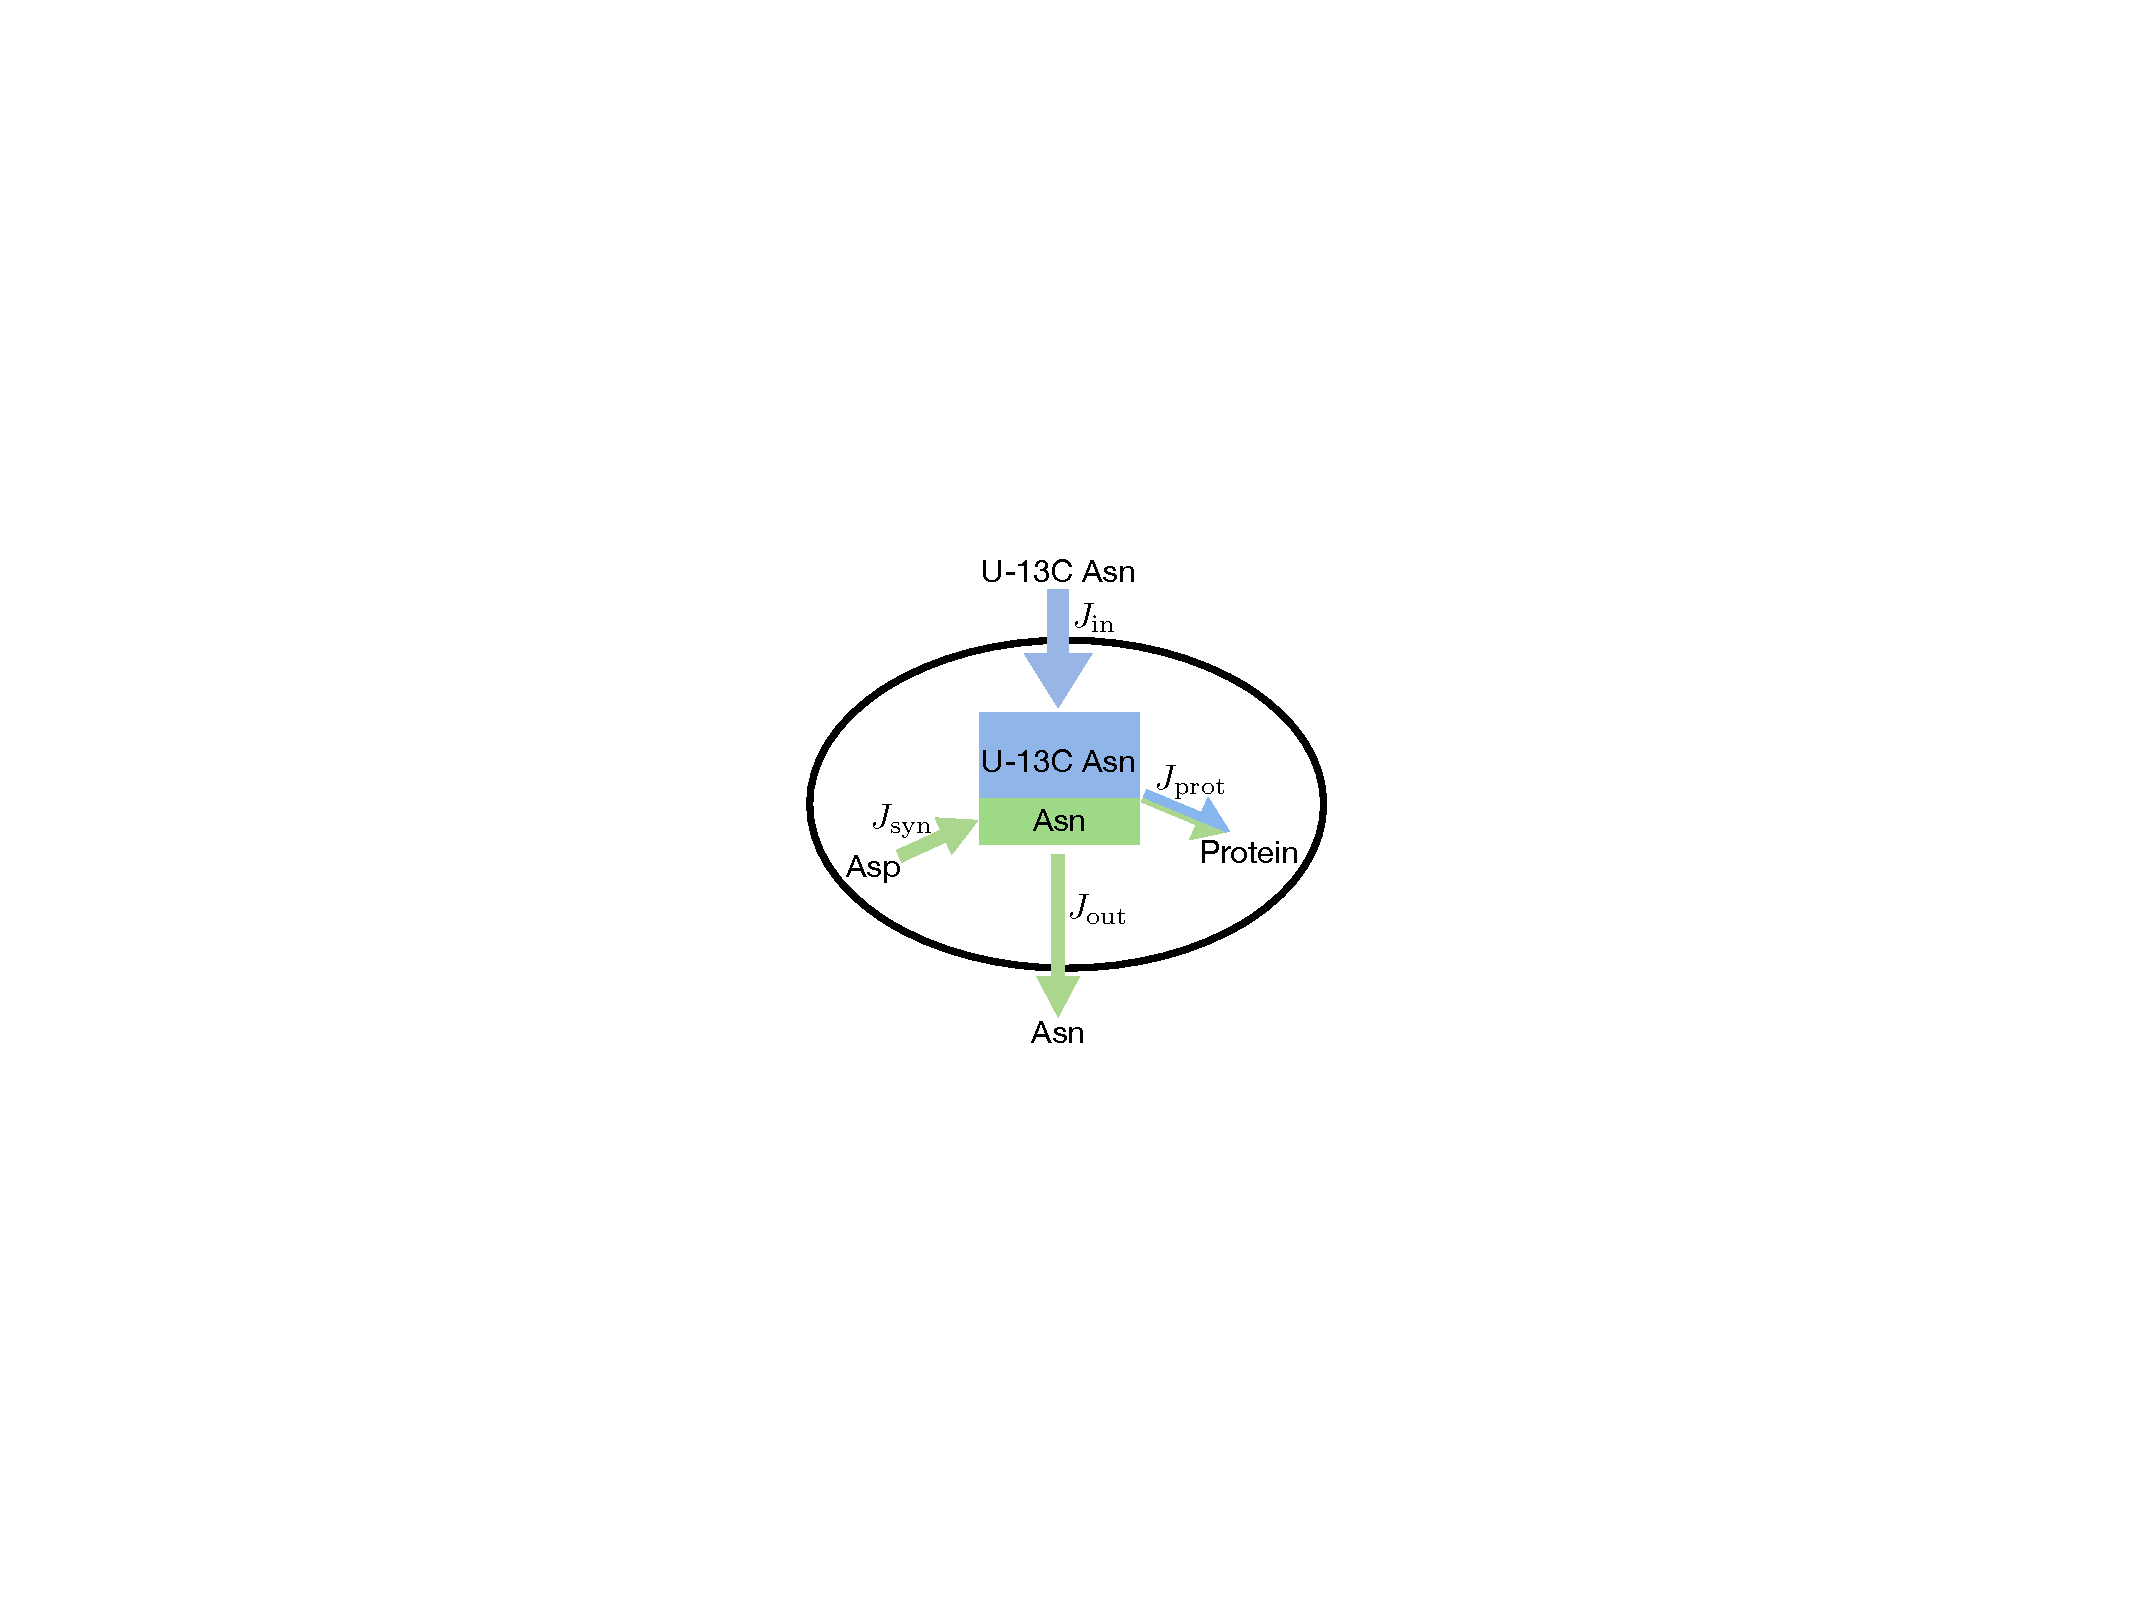
\includegraphics[width=\textwidth]{figures/chap2/asn_Jprot.pdf}
         \caption{Flux diagram}
         \label{fig:ch2:asn_Jprot}
     \end{subfigure}
     \hfill
     \begin{subfigure}[b]{0.4\textwidth}
         \centering
         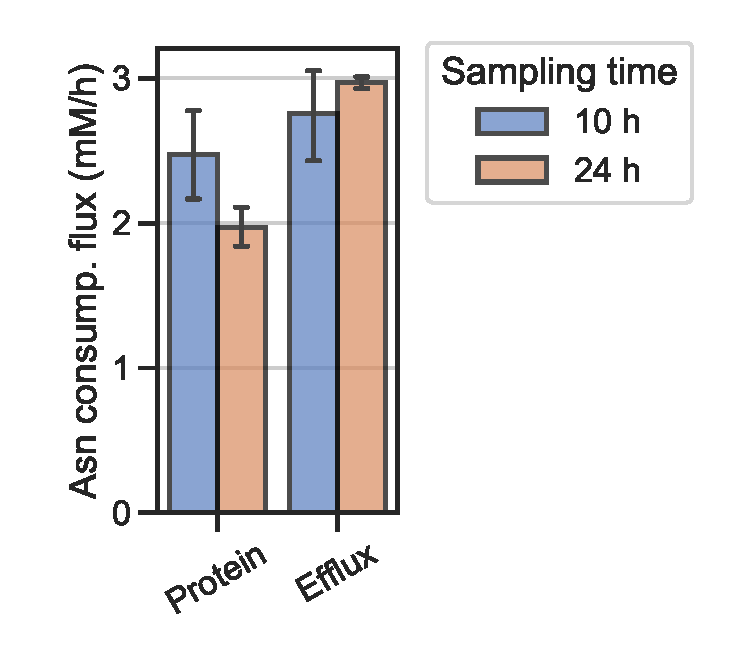
\includegraphics[width=\textwidth]{figures/chap2/Asn_flux.pdf}
         \caption{Asn consumption}
         \label{fig:ch2:Asn_flux}
     \end{subfigure}
     \hspace{0.05\textwidth}
        \caption[Asparagine consumption fluxes]{
        (a) Diagram of asparagine fluxes in a cell.
        Net influx of U-\hCi{} labelled Asn ($\Flin$), net efflux of unlabelled Asn ($\Flout$), net deposition of Asn into protein ($\Flprot$) and Asn synthesis from Asp ($\Flsyn$).
        Asn symbolized by green and U-\hCi{} Asn symbolized by blue.
        (b) Measured asparagine consumption fluxes in 143B cells using the media uptake data from figure \ref{fig:ch2:flux_143wt}.
        Asn is consumed into protein synthesis (Protein) and leaked into the media (Efflux).
        Efflux is calculated assuming no Asn is provided in the media.
        }
\end{figure}



Most of cellular biomass is amino acids \cite{Hosios2016-us}

\begin{figure}
    \centering
    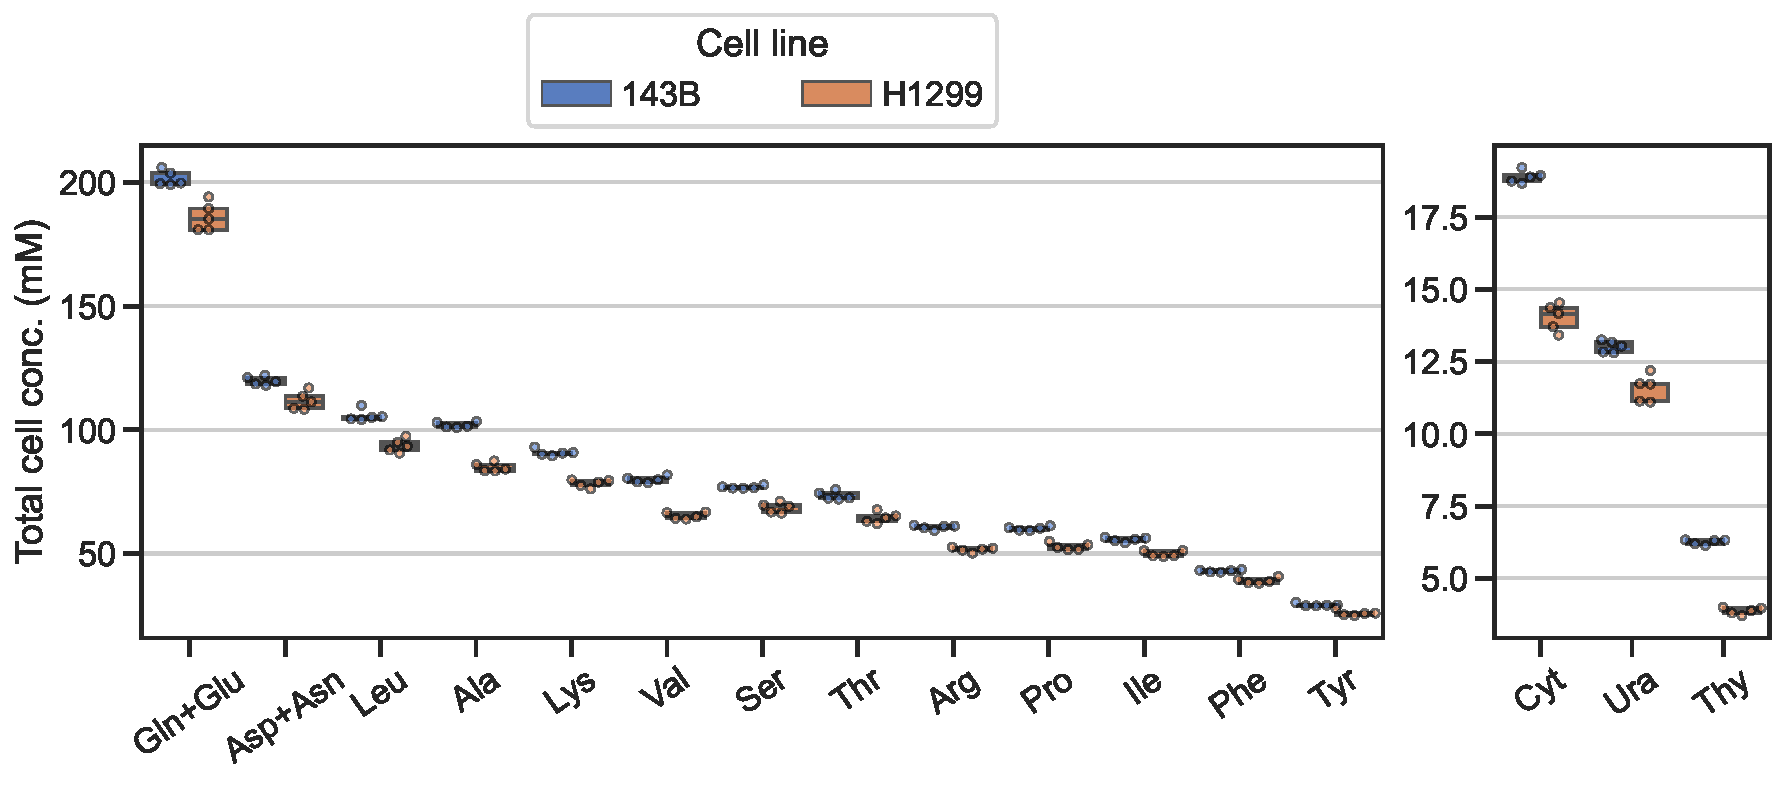
\includegraphics[width=0.80\textwidth]{figures/chap2/ah_cell_comp.pdf}
    \caption[Amino acid and pyrimidine total cell concentration]{
    Total amino acids and pyrimidines liberated by acid hydrolysis of 143B and H1299 cells, normalized by total cell volume (Total cell conc.).
    Gln and Asn is converted during acid hydrolysis to Glu and Asp respectively.
    }
    \label{fig:ch2:ah_cell_comp}
\end{figure}






The total Asp consumption flux expected in DMEM i.e. with Arg but without Asn, is estimated to be 9.25 mM/h.
This is close to Asp uptake in 143B GOT DKO which was measured at 11.43 mM/h (figure \ref{fig:ch2:flux_143dko}).
The difference is directionally as would be expected because total pyrimidine/purine levels underestimate synthesis flux by discounting recycling (figure ]\ref{fig:ch2:pur_tr_ov}) and because 143B GOT DKO maintain a higher intracellular concentration of aspartate due to expression of Glu/Asp transporter SLC1A3.
\begin{figure}
    \centering
    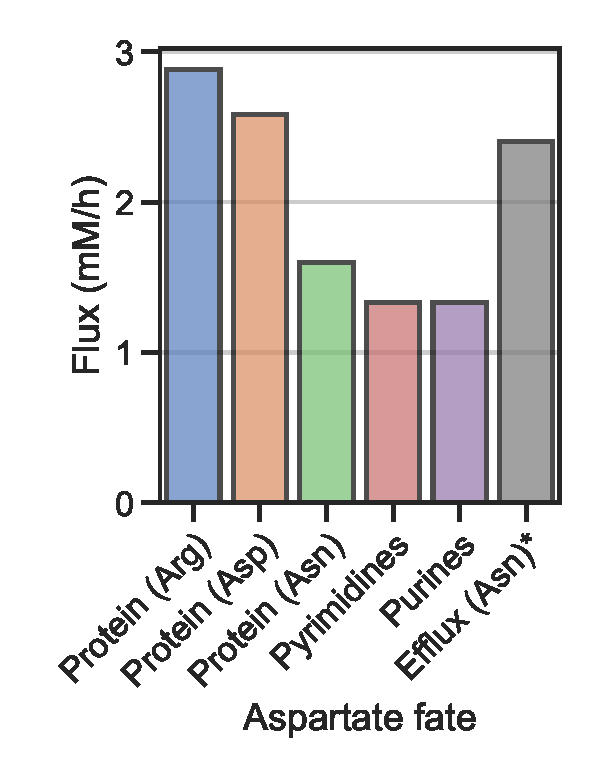
\includegraphics[width=0.36\textwidth]{figures/chap2/asp_fate.pdf}
    \caption[Relative consumption towards each fate of aspartate]{
    Relative consumption towards each fate of aspartate estimated using best estimates from figure \ref{fig:ch2:Asn_flux} and \ref{fig:ch2:ah_cell_comp}.
    Aspartate consumption towards purines was estimated equal to consumption towards pyrimidines.
    * Asn efflux is calculated based on the assumption that cells are grown in asparagine free media, prior to substantial media conditioning.
    }
    \label{fig:ch2:asp_fate}
\end{figure}






\section{Salvage of the metabolic fates of aspartate}

\subsection{Salvage mix fulfills all the metabolic fates of aspartate}

metabolic fates of aspartate i.e. aspartate conversion 


\begin{figure}
    \centering
    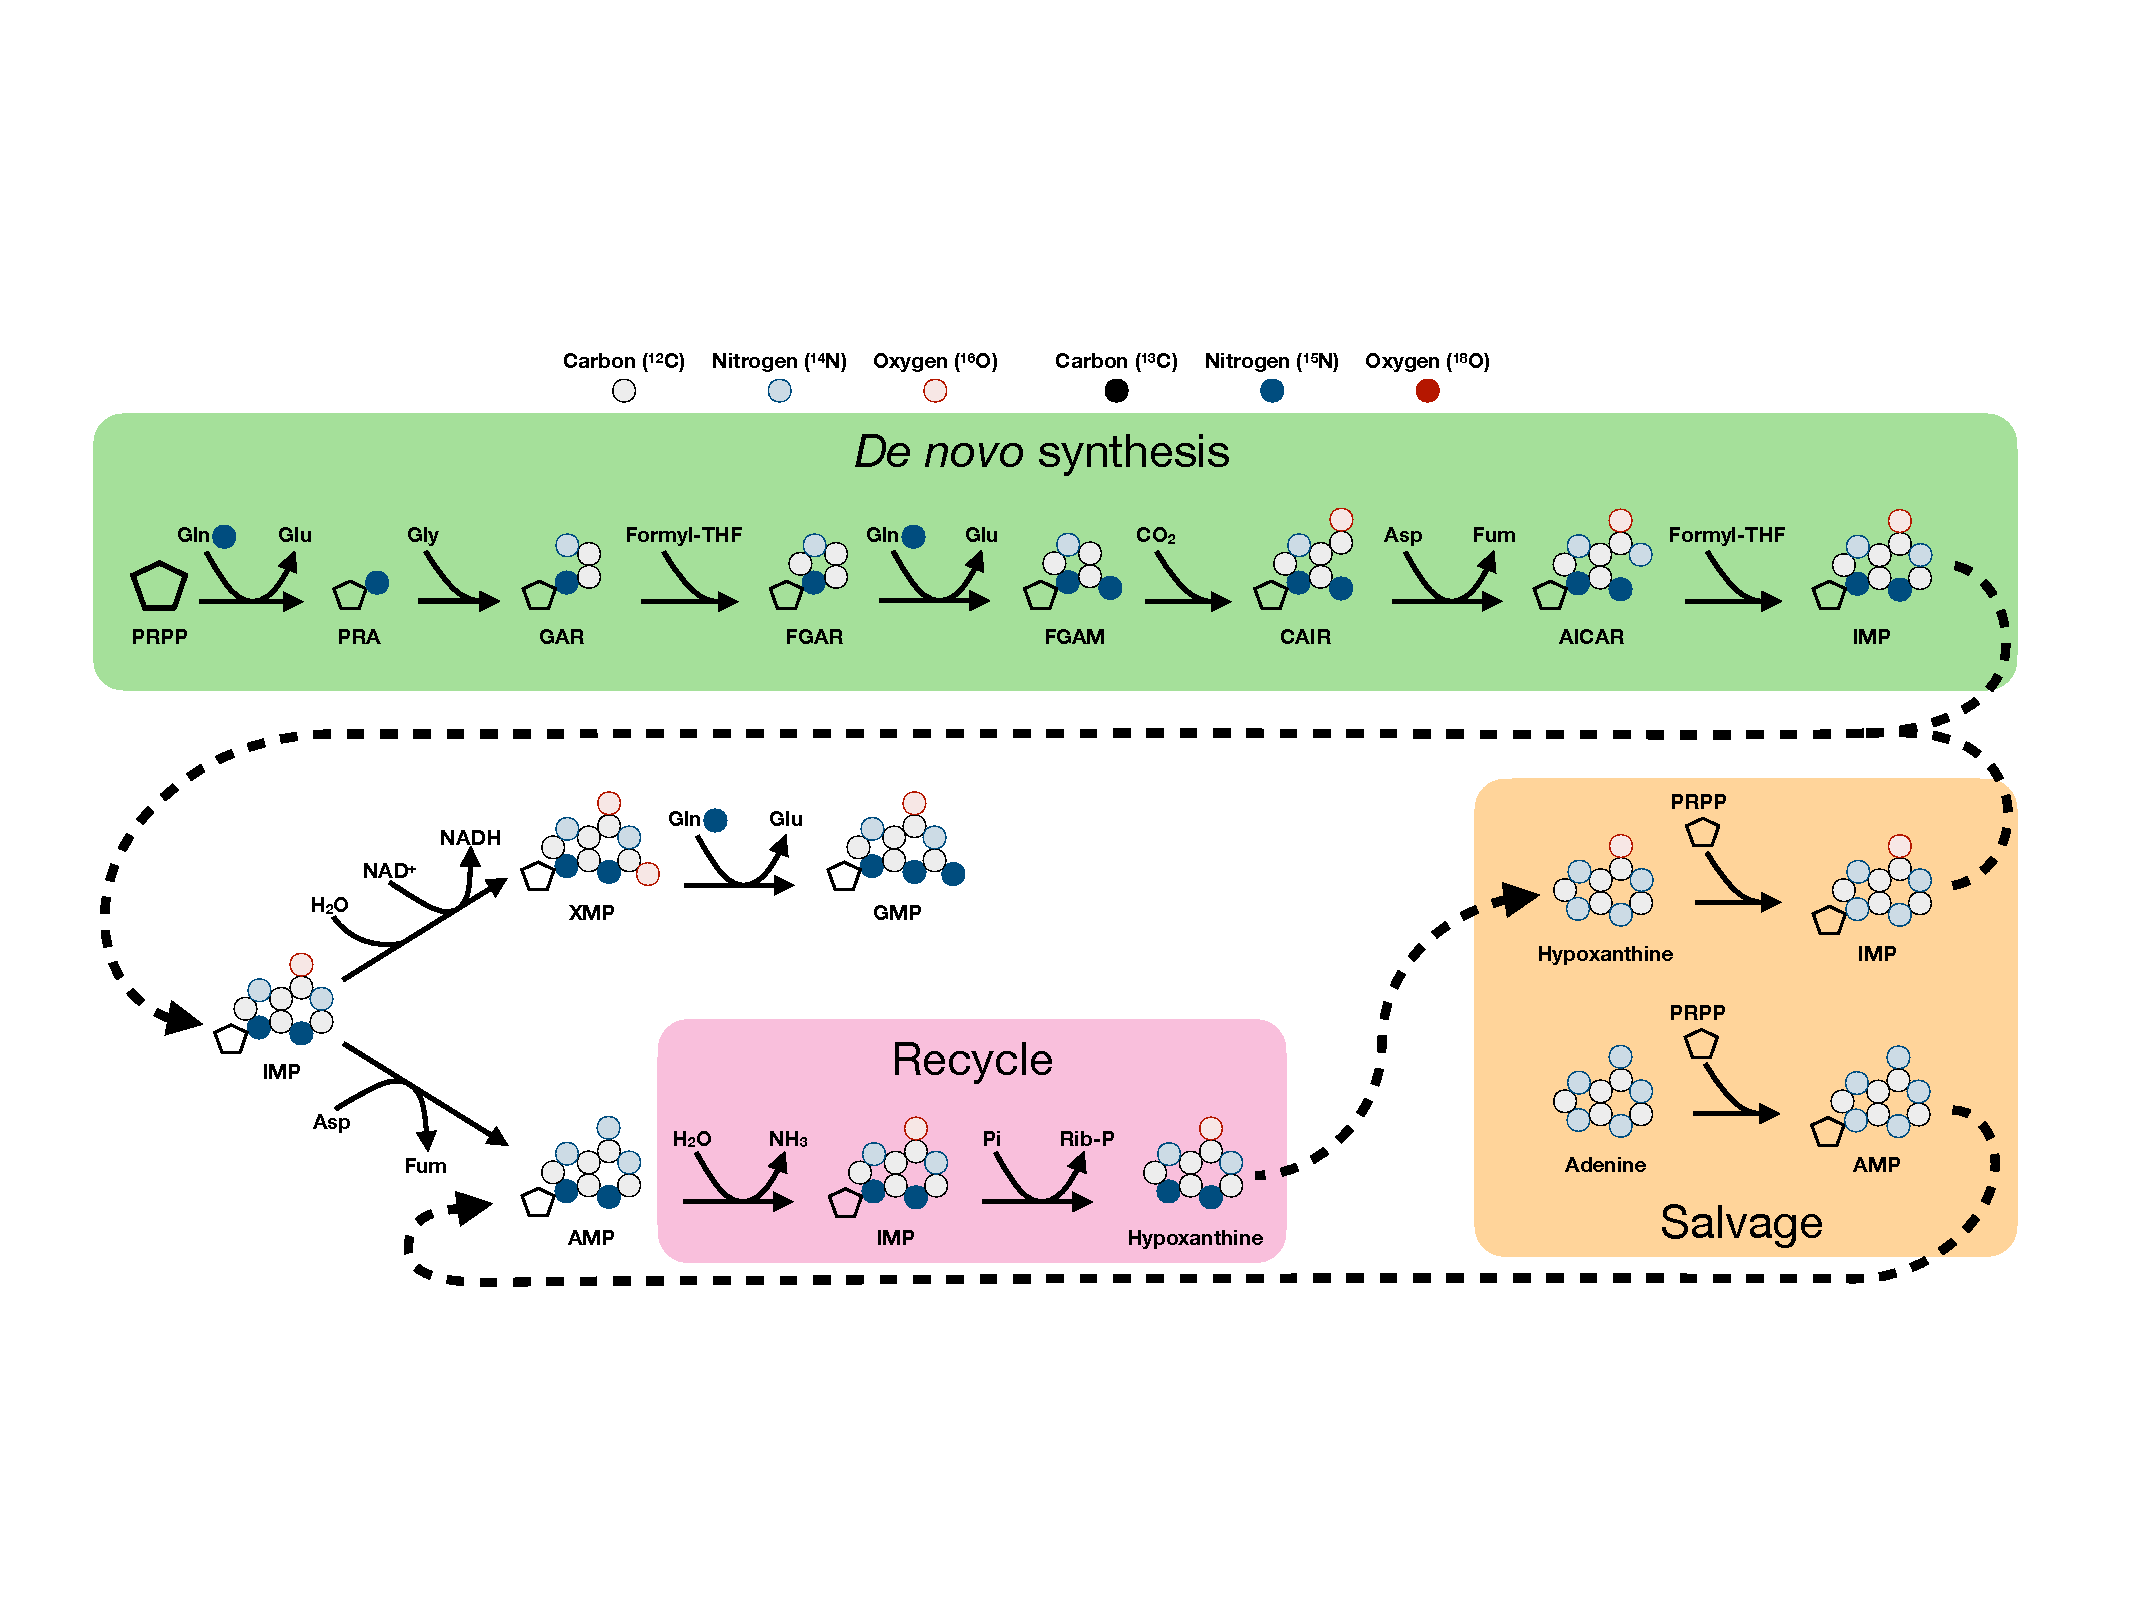
\includegraphics[width=0.95\textwidth]{figures/chap2/purine_tracing_overvew.pdf}
    \caption[Purine metabolism \hNi-amide Gln tracing overview]{
    Overview of \hNi-amide Gln label incorporation in \textit{de novo} purine synthesis.
    Label incorporation can be effected by salvage of unlabelled hypoxanthine or adenine and recycling as it appears on the overview.
    }
    \label{fig:ch2:pur_tr_ov}
\end{figure}





\begin{figure}
    \centering
    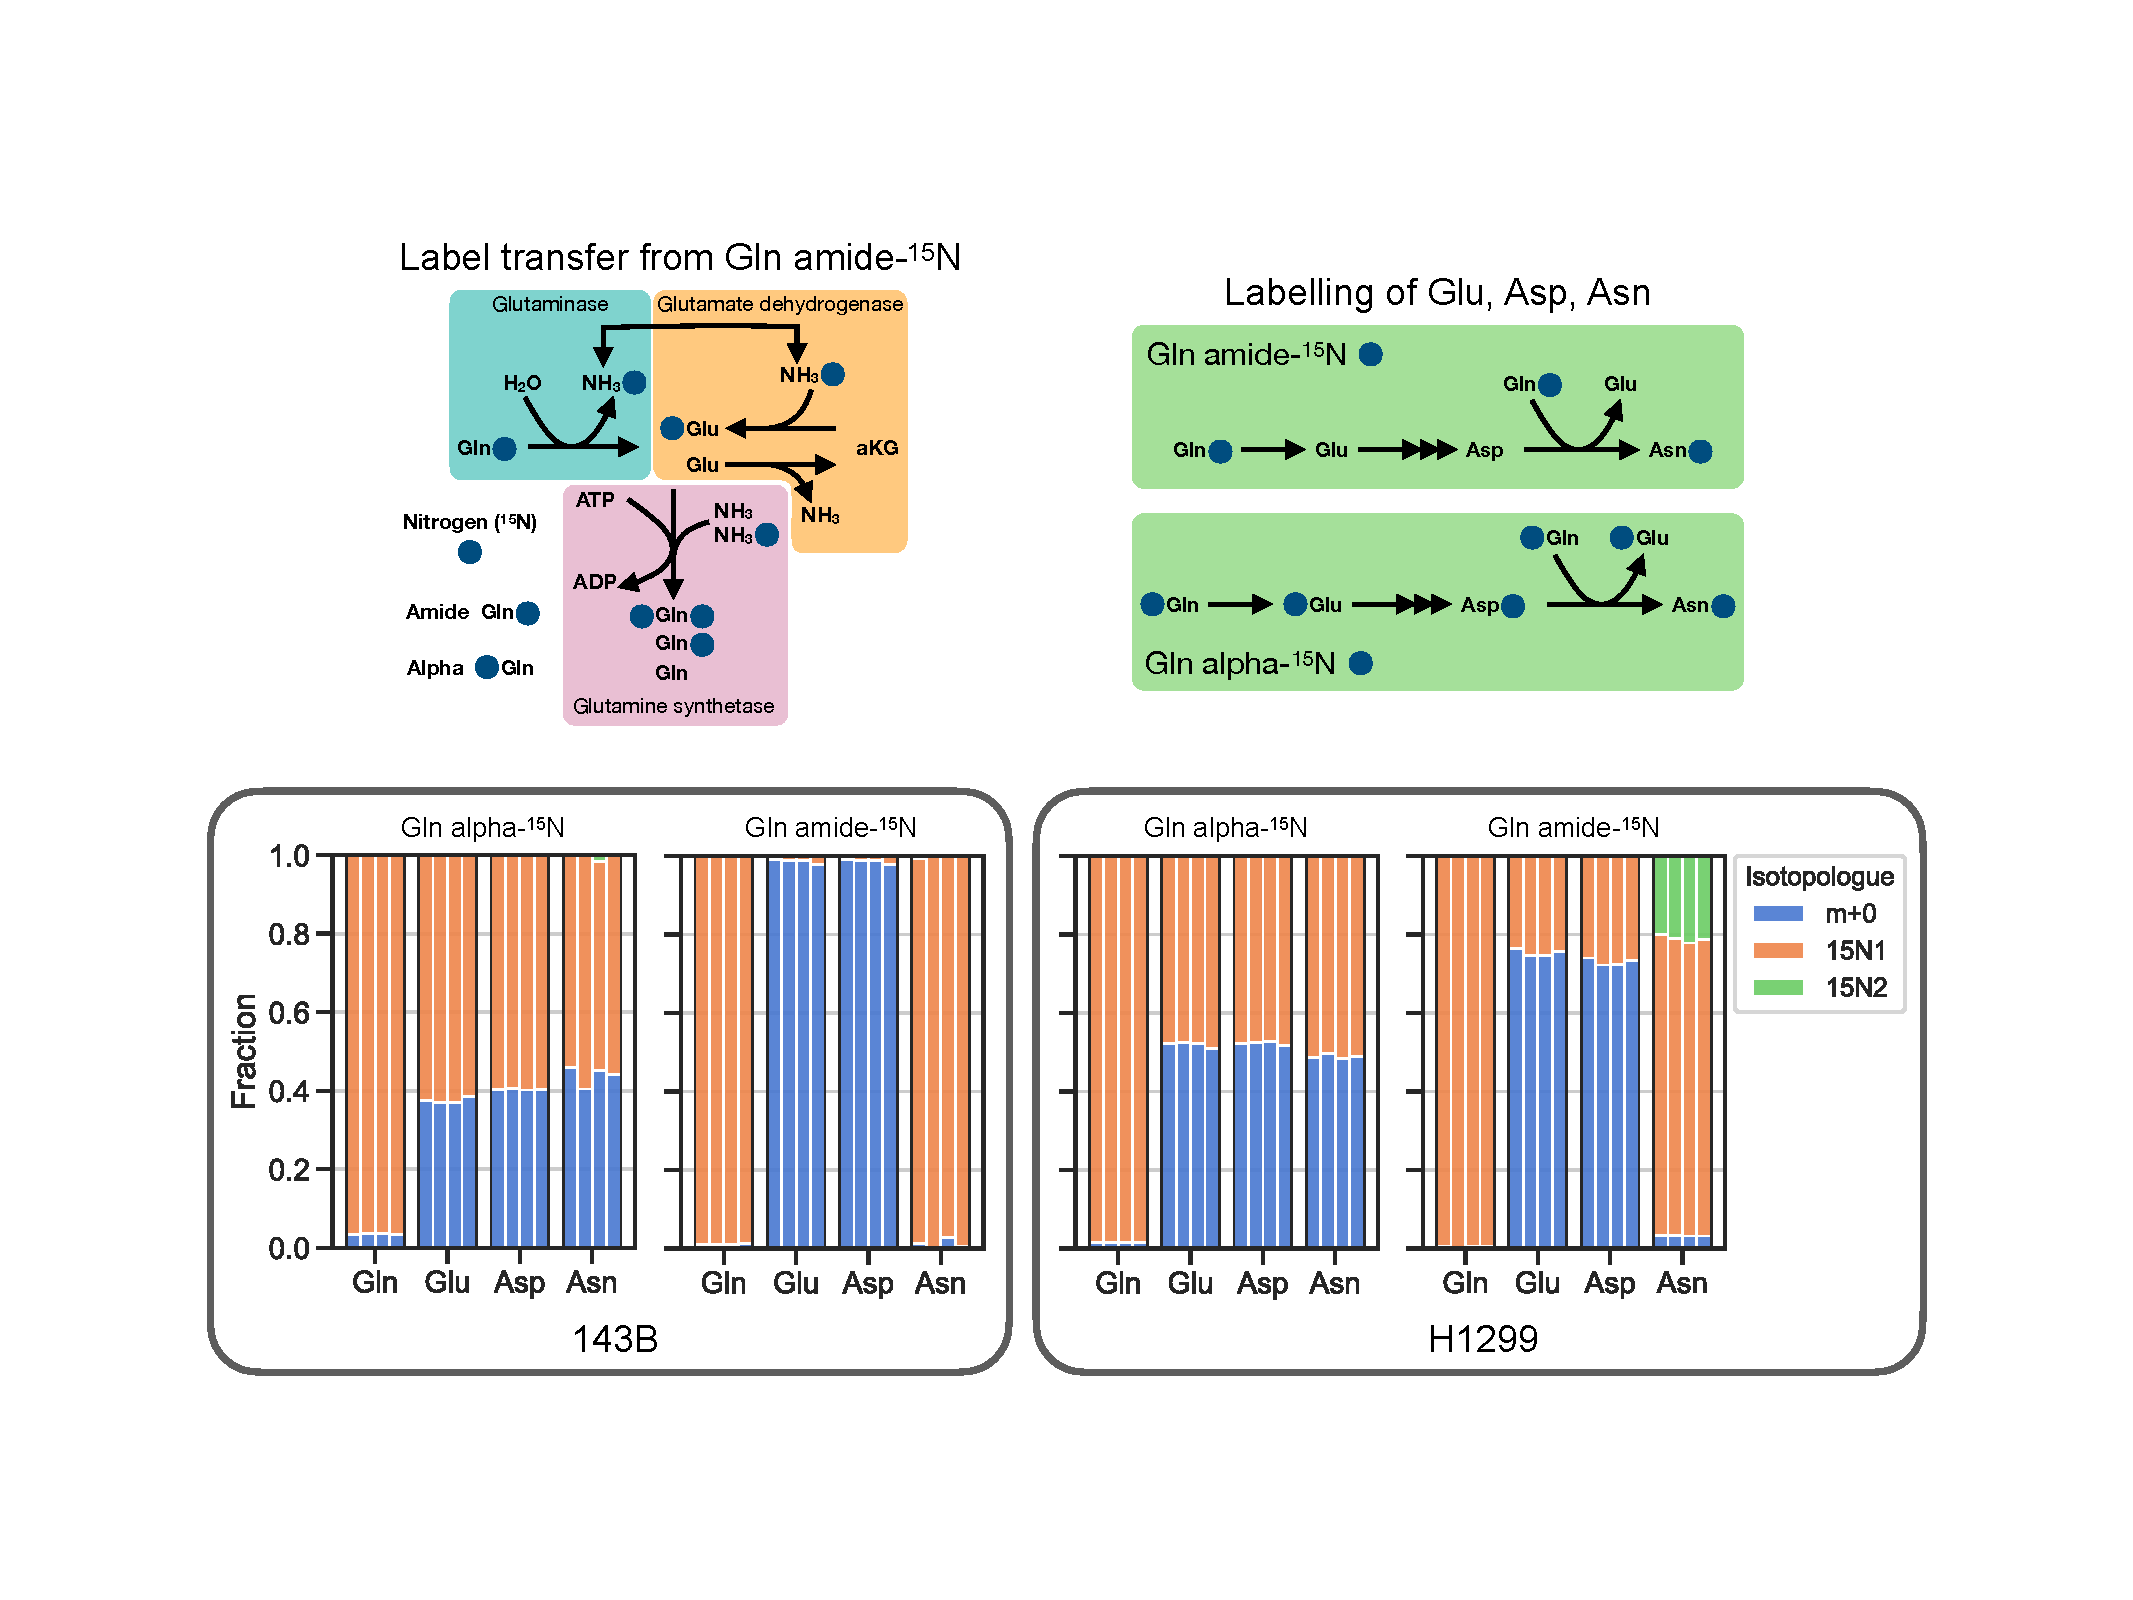
\includegraphics[width=0.95\textwidth]{figures/chap2/gln_lab_tranfr.pdf}
    \caption[Gln amide to alpha \hNi{} transfer]{
    Gln \hNi{} on the amide nitrogen can transfer to the alpha nitrogen in H1299 cells but not in 143B cells.
    Upper left diagram shows how Gln amide and alpha nitrogen labels can transfer.
    Transfer of amide labelled nitrogen can be achieved by glutaminase catalyzed release of labelled ammonia and its subsequent use as a substrate in the conversion of alpha-ketoglutarate (aKG) to Glu alpha-\hNi by glutamate dehydrogenase.
    The signature of glutamine synthetase activity is the appearance of doubly labelled Gln.
    Upper right diagram shows how Gln amide and alpha nitrogen labels are transferred to downstream metabolites Glu, Asp and Asn.
    Lower panel shows the nitrogen isotopologue distribution of Gln, Glu, Asp and Asn in 143B and H1299 at steady-state.
    The alpha nitrogen label is frequently lost in Glu and downstream, presumably due to transaminase catalyzed exchange with unlabelled amino groups on amino acids such as leucine, isoleucine, valine etc.
    The amide nitrogen label is partially transferred to the alpha position in H1299, but not in 143B, also indicated by the doubly labelled Asn.
    }
    \label{fig:ch2:gln_lab_tranfr}
\end{figure}


\begin{figure}
    \centering
    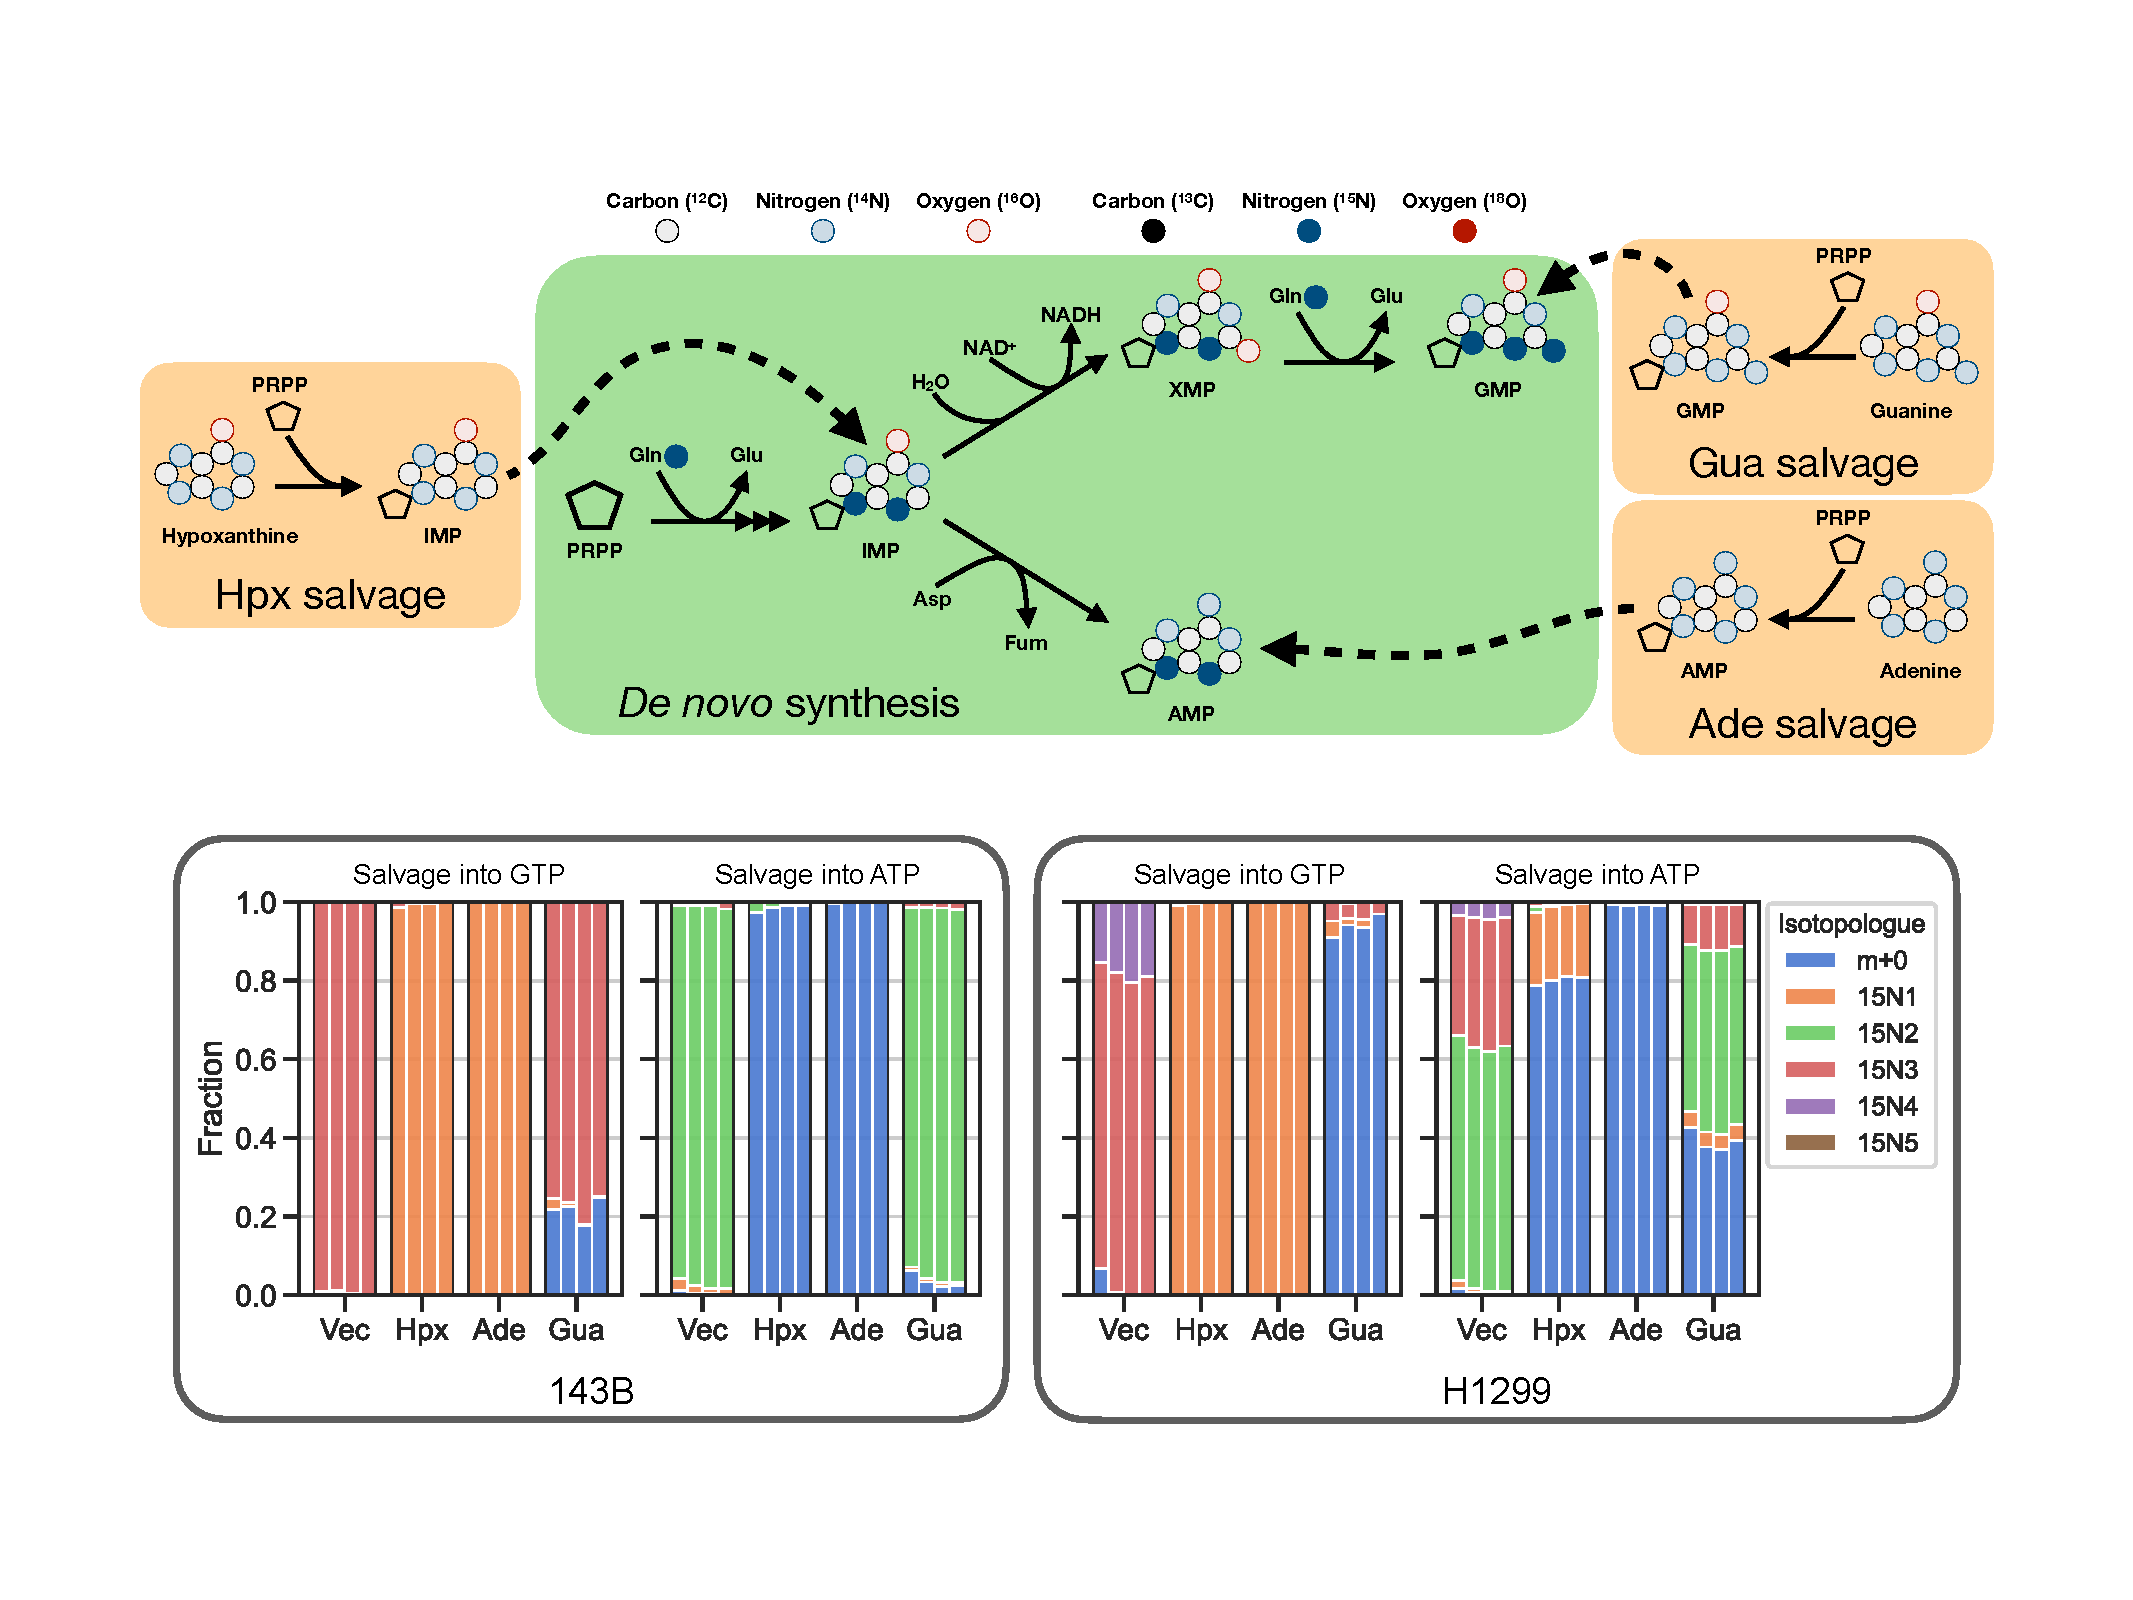
\includegraphics[width=0.98\textwidth]{figures/chap2/sal_frac_pur.pdf}
    \caption[Salvage into purines]{
    ggg
    }
    \label{fig:ch2:sal_frac_pur}
\end{figure}


\begin{figure}
    \centering
    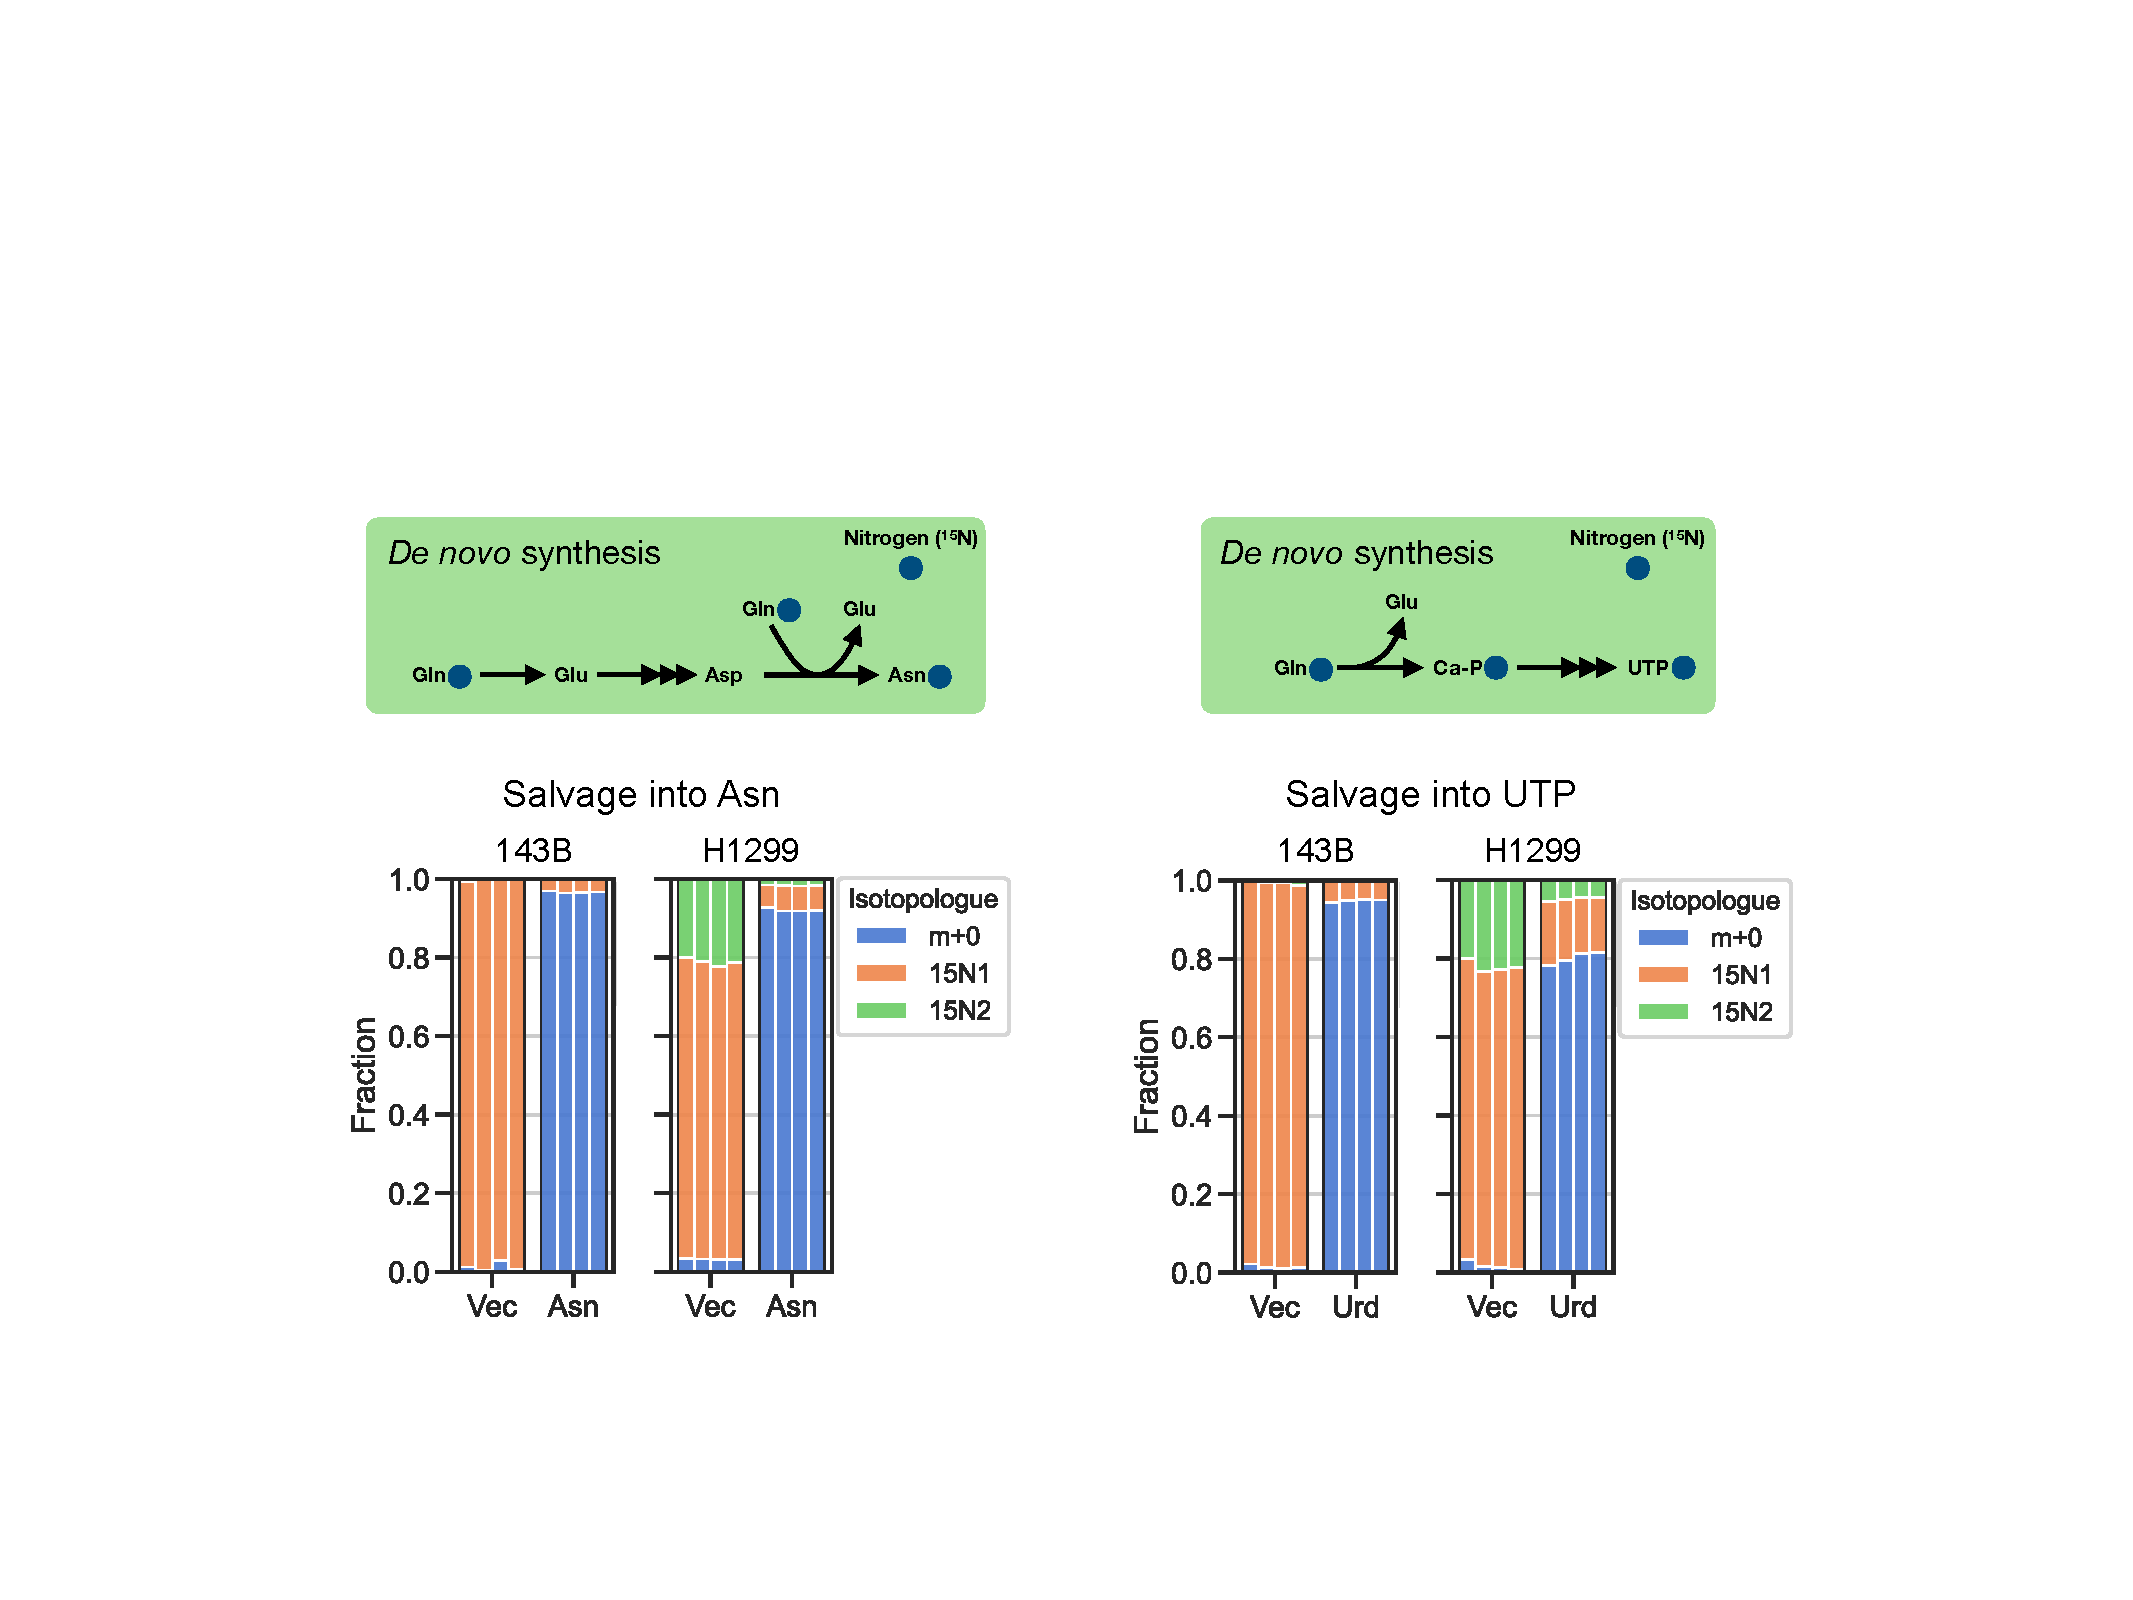
\includegraphics[width=0.8\textwidth]{figures/chap2/sal_frac_pyr-asn.pdf}
    \caption[Salvage into asparagine and pyrimidines]{
    ggg
    }
    \label{fig:ch2:sal_frac_pyr-asn}
\end{figure}









\begin{figure}
    \centering
    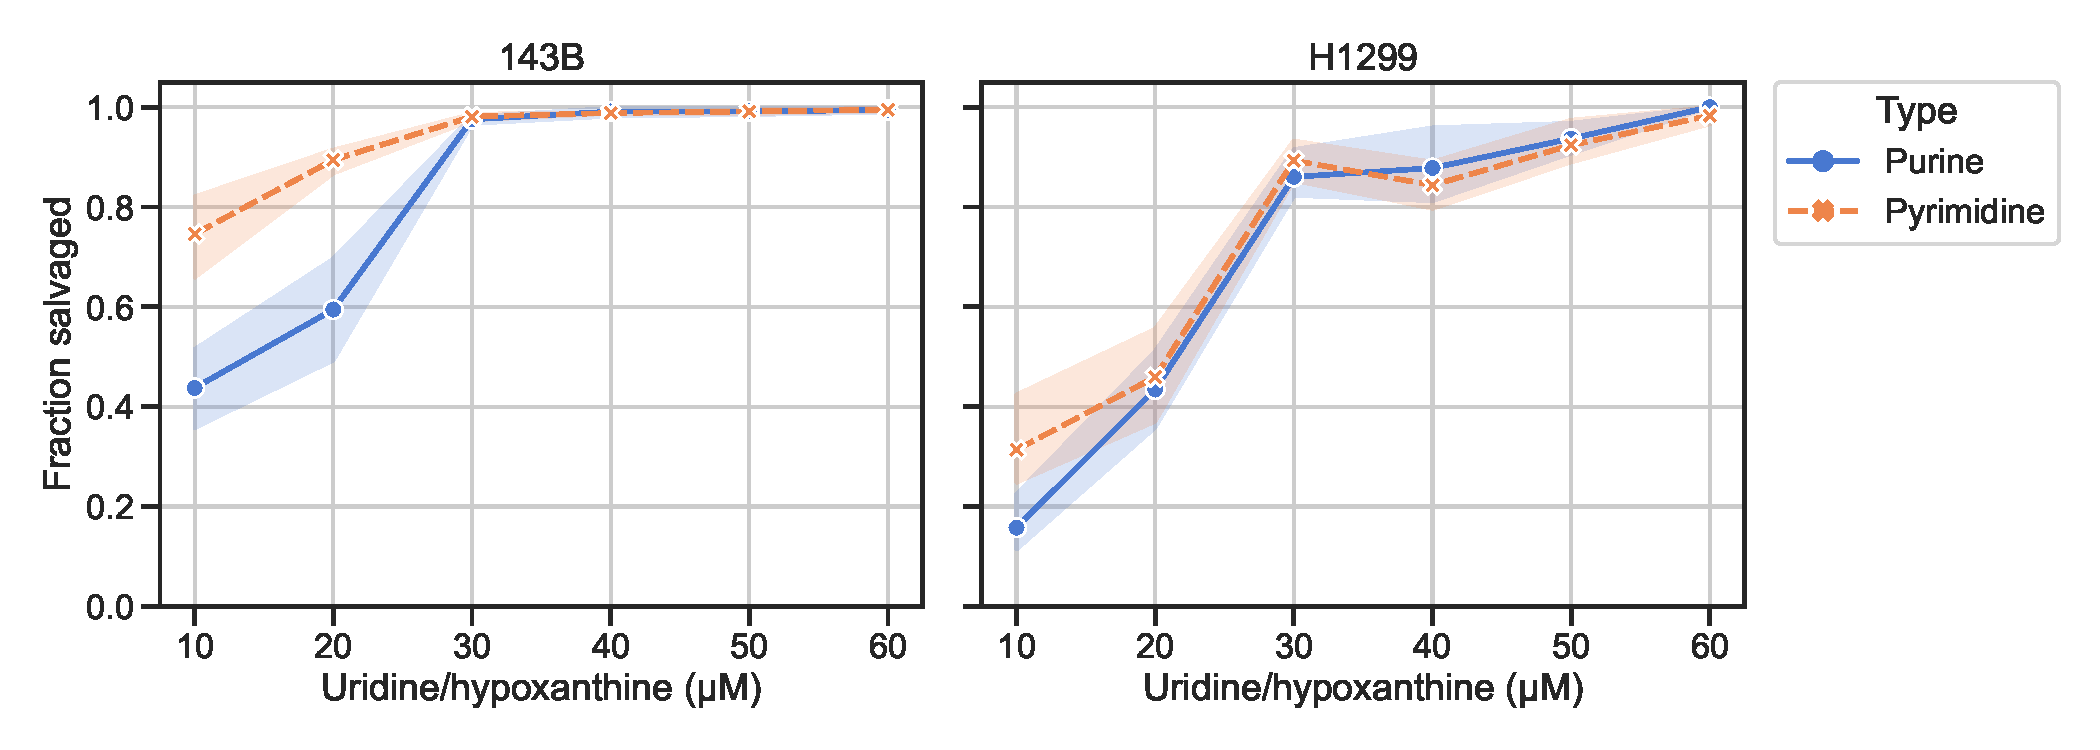
\includegraphics[width=0.95\textwidth]{figures/chap2/sal_frac_conc.pdf}
    \caption[Salvage as a function of Urd/Hpx concentration]{
    Fraction of purines (GDP, GMP, ADP and AMP) and pyrimidines (UDP, UMP, CDP and CMP) derived from salvage when 143B or H1299 cells are cultured in increasing concentrations of uridine/hypoxanthine.
    }
    \label{fig:ch2:sal_frac_conc}
\end{figure}







\section{Aspartate to proliferation curves}

%%% Experiments with individual components under "ETCrescue" folder in lab-work

%%% Experiments with H1299 (Metformin and Rotenone) and HT1080




\section{Integrated stress response}

Overlap between perturbations eliciting ISR by GCN2 and HRI \cite{Taniuchi2016-nc}









\section{Methods and Materials}

\subsection{Cell culture}
Cell lines were acquired from ATCC (143B, H1299, HT1080) and tested to be free from mycoplasma (MycoProbe, R\&D Systems).
Cells were maintained in Dulbecco’s Modified Eagle’s Medium (DMEM) (Gibco, 50-003-PB) supplemented with 3.7 g/L sodium bicarbonate (Sigma, S6297), 10\% fetal bovine serum (FBS) (Gibco, 26140079) and 1\% penicillin-streptomycin solution (Sigma, P4333).
Cells were incubated in a humidified incubator at 37°C with 5\% CO2.


\subsection{Western blots}
Protein lysates were harvested in RIPA buffer (Sigma, R0278) supplemented with Halt protease and phosphatase inhibitor cocktail (Fisher, PI78443) and 5 mM EDTA.
Protein concentration was determined using a bicinchoninic acid assay (Fisher, 23225) using bovine serum albumin (BSA) as a protein standard.
Equal amounts of protein were added to LDS sample buffer (ThermoFisher, B0008) and 5\% 2-Mercaptoethanol (Sigma, M3148), denatured at 95°C for 5 min, loaded onto 4–12\% SDS-polyacrylamide gels (Invitrogen, NW04122BOX) along with a prestained protein ladder (ThermoFisher, 26616) and run 35 min at 180V in MES buffer (ThermoFisher, B000202).
Proteins were dry transferred onto a 0.22 mm nitrocellulose membranes using the iBlot2 device (ThermoFisher, IB21001) with the P0 system setting and associated transfer stacks (Fisher, IB23001).
Membranes were blocked with 5\% bovine serum albumin; Sigma, A4503 in tris-buffered saline with 0.1\% Tween-20 (TBS-T) and incubated at 4°C overnight with the following antibodies:
anti-ATF4 (Cell Signaling, 11815S, 1:500),
anti-ASNS (Cell Signaling, 92479T, 1:1000),
anti-Phospho-eIF2alpha (Cell Signaling, 3398S, 1:500),
anti-eIF2alpha (Cell Signaling, 5324S, 1:500),
anti-Phospho-GCN2 (Cell Signaling, 94668S, 1:500),
anti-GCN2 (Cell Signaling, 3302S, 1:500),
anti-OMA1 (Cell Signaling, 95473, 1:1000),
anti-GADD34 (Proteintech, 10449-1-AP, 1:500),
anti-DARS2 (Proteintech, 13807-1-AP, 1:500),
anti-HRI (Sigma, HPA016496, 1:1000),
anti-FLAG (Sigma, F1804; 1:1000),
anti-SLC1A3 (Genetex, GTX20262; 1:500),
anti-GOT2 (Proteintech, 14800–1-AP, 1:750),
anti-GOT1 (Cell Signaling, 34423 S, 1:1000),
anti-Vinculin (Sigma, SAB4200729; 1:10,000) and anti-Tubulin (Sigma, T6199; 1:10,000).
Membranes were washed with TBS-T and the following secondary antibodies were added in blocking buffer: 800CW Goat anti-Mouse IgG (LiCOR, 926–32210; 1:15,000), 680RD Goat anti-Rabbit IgG (LiCOR, 926–68071; 1:15,000) and incubated for 1 hour.
Membranes were washed with TBS-T, incubated for 10 min in TBS-T, washed in deionized water and imaged on a LiCOR Odyssey Near-Infrared imaging system.


\subsection{Proliferation assays}
Cells were trypsinized (Corning, 25,051 CI), resuspended in seeding media, counted (Beckman Coulter Counter Multisizer 4) and seeded overnight onto 6/12/24-well dishes (Corning, 3516;3513:3524) with an initial seeding density of 10,000 cells/mL and a volume of 4, 2 and 1 mL, respectively.
After overnight incubation, 3–6 wells were counted for a starting cell count at the time of treatment.
Treatment was initiated either by media switch or by spike-in of drug/metabolite from a 20-50x stock.
Experiments were conducted in (both for seeding and treatment) DMEM without pyruvate (Corning 50–013-PB) supplemented with 3.7 g/L sodium bicarbonate 10\% dialyzed fetal bovine serum (FBS) (Sigma, F0392) and 1\% penicillin-streptomycin solution, with or without sodium pyruvate (Pyr) (Sigma, P8574),
2-ketobutyric acid (AKB) (Sigma, K401),
aspartate (Asp) (Sigma, A7219),
asparagine (Asn) (Sigma, A7094),
uridine (Urd) (Sigma, U3003), hypoxanthine (Cayman Chemical, 22254),
adenine (Ade) (Sigma, A2786),
guanine (Gua) (Sigma, 51030) or sodium formate (Sigma, 71539) with concentration noted when relevant.
Drug treatments included rotenone (Sigma, R8875),
metformin (Sigma, D150959),
atpenin A5 (Cayman Chemical, 11898; AdipoGen, AG-CN2-0110; Abcam, ab144194; or Enzo Life Sciences, ALX-380–313),
doxycycline hydrochloride (Sigma, D3447),
antimycin A (Sigma, A8674),
oligomycin A (Sigma, 495455),
GCN2iB (MedChemExpress, HY-112654),
FCCP (Cayman Chemical, 15218-10),
BAM15 (Cayman Chemical, 17811),
UCPH (HelloBio, HB0630) and DMSO vehicle (Sigma, D2650).
Cells were incubated in a humidified incubator at 37°C with 5\% CO2, then counted after 4–6 days.
Proliferation rate was reported as doublings per day and determined using the time and fold count difference between the starting and final counts and assuming a constant proliferation rate throughout the assay.


\subsection{Generation of nuclear RFP cell lines}
Nuclear RFP cell lines were generated using 1e5 transducing units of EF1A-nuclear RFP lentivirus (Cellomics Technology, PLV-10205-50) by spinfection.
Cells were seeded at 50\% confluency on 6 well dishes, lentivirus was added to fresh media with 8 µg/µL polybrene, then added to cells and followed by centrifugation (900g, 90 mins, 30°C).
Two days after infection, cells were sorted for high RFP expression using fluorescence-activated cell sorting (FACS).
High RFP cells were then expanded and single-cell cloned by limiting dilution, plating 0.5 cells/well on a 96 well plate.
Plates were then screened for RFP expression and localization using Incucyte S3 (Sartorius) and a suitable clone chosen, expanded, and used for all subsequent experiments.


\subsection{Incucyte measurements}
Proliferation assay using Incucyte



\subsection{Lentiviral production and stable cell line generation}
The following plasmids were obtained: pLenti6.3-V5 DEST\_SLC1A3 (DNASU Plasmid Repository), ATF4 reporter pXG237 (Addgene, 141281), pLHCX-gpASNase1 (Addgene, 121526) and pDONR221\_EGFP (Addgene, 25899).
ASNS was cloned by PCR from HEK293T reverse transcribed mRNA.
Genes were first cloned into entry vector pENTR1A (Fisher, A10462) using NEBuilder HiFI DNA Assembly Cloning Kit (New England BioLabs, E2621).
These donor constructs were then used to transfer their insert into destination vectors: pLX304-CMV-Blast (Addgene, 25890) or pLenti-CMV-Hygro (w117-1) (Addgene, 17454 a gift from Eric Campeau \& Paul Kaufman) using LR Clonase II (Fisher, 11791100).
Each plasmid sequence was verified by whole plasmid sequencing (Plasmidsaurus).
Lentivirus was generated by co-transfection of HEK293T cells with destination vector plasmid DNA and the packaging plasmids pMDLg/pRRE (Addgene, 12251), pRSV-Rev, (Addgene, 12253) and pMD2.G (Addgene, 12259) using FuGENE transfection reagent (Fisher, PRE2693) in DMEM (Fisher, MT10017CV) without FBS or penicillin-streptomycin.
The supernatant containing lentiviral particles was filtered through a 0.45 µM membrane (Fisher, 9720514) and was supplemented with 8 µg/µL polybrene (Sigma, TR-1003-G) prior to infection.
For infection, cells were seeded at 50\% confluency in 6 well dishes and centrifuged with lentivirus (900g, 90 mins, 30°C).
After 24 hours the media was replaced with fresh media and after 48 hours cells were treated with either 1 µg/mL blasticidin (Fisher, R21001) or 150 µg/mL hygromycin (Sigma, H7772-1G) and maintained in selection media until all uninfected control cells died.
After selection, cells were expanded and single-cell cloned by limiting dilution, plating 0.5 cells/well using 96 well plates.
These clones were expanded and screened by either western blot or presence of GFP or RFP signal using Incucyte S3 (Sartorius) to validate expression.
From this a single clone was chosen, expanded and used for all subsequent experiments.


\subsection{Generation of knockout cells}
Protocol and guide RNA generation was identical to that described in Hart et al. \cite{Hart2023-gp}.
Briefly, three chemically synthesized 2'-O-methyl 3’phosphorothioate-modified single guide RNA (sgRNA) sequences targeting the gene of interest were purchased (Synthego; table \ref{tab:ch2:guides}).
A pool of all three sgRNAs (or all six for GOT1/GOT2 double knockout) were resuspended in nuclease-free water, combined with SF buffer (Lonza, V4XC-2032), and sNLS-spCas9 (Aldevron, 9212).
200,000 H1299 cells were resuspended in the resulting solution containing ribonucleoprotein complexes (RNPs) and electroporated using a 4D-Nucleofector (Amaxa, Lonza).
Nucleofected cells were then expanded and single-cell cloned by limiting dilution by plating 0.5 cells/well in a 96 well plate.
Gene knockout was confirmed using western blots.

\begin{spacing}{1}
\begin{table}[ht]
\caption{\label{tab:ch2:guides}CRISPR guides.}
\begin{tabular}{|l|l|}
\hline
Gene & sgRNA   sequence (5’-3’) \\
\hline
GOT1 & \begin{tabular}[c]{@{}l@{}}\texttt{CAGUCAUCCGUGCGAUAUGC}\\\texttt{GCACGGAUGACUGCCAUCCC}\\\texttt{CGAUCUUCUCCAUCUGGGAA}\end{tabular} \\
\hline
GOT2 & \begin{tabular}[c]{@{}l@{}}\texttt{UUUCUCAUUUCAGCUCCUGG}\\\texttt{CGGACGCUAGGCAGAACGUA}\\\texttt{UCCUUCCACUGUUCCGGACG}\end{tabular} \\
\hline
OMA1 & \begin{tabular}[c]{@{}l@{}}\texttt{ACACAUUAGCAUCCACCUCA}\\\texttt{GAGUAAAUCAGUGUGACAGG}\\\texttt{GCCAACCCAAGAUGCCAGAA}\end{tabular} \\
\hline
HRI & \begin{tabular}[c]{@{}l@{}}\texttt{GUUUGCAACUGCAAAAGGGA}\\\texttt{UGAUGUUCCAGCAGAAAUCC}\\\texttt{CCAGCACCUUCACUUCCCGU}\end{tabular} \\
\hline
GCN2 & \begin{tabular}[c]{@{}l@{}}\texttt{AAAACUAAAUUGAUUUCAGG}\\\texttt{AGCUCGGUCAUCCUUGGCCA}\\\texttt{GAACUGGCCAAGAAACACUG}\end{tabular} \\
\hline
SLC25A10 & \begin{tabular}[c]{@{}l@{}}\texttt{GCAUCUGCAGACGCAGCAGG}\\\texttt{GCAACACCUUCUCGUGGAAG}\\\texttt{GAAGCUGCGCAUGACGGGCA}\end{tabular} \\
\hline
DARS2 & \begin{tabular}[c]{@{}l@{}}\texttt{ACAUAAAAUCUUCUUCACAG}\\\texttt{UGGUUAAGUCAGCUGUACAG}\\\texttt{GUGGAUGGAUUCAGUACCGA}\end{tabular} \\
\hline
\end{tabular}
\end{table}
\end{spacing}

\subsection{Polar metabolite extraction}
For polar metabolite extraction, a plate was move to ice and the media was thoroughly aspirated.
Wells were washed thrice with cold saline (Fisher, 23293184), 1 mL 80\% HPLC grade methanol in HPLC grade water was added, cells were scraped with the back of a P1000 pipet tip and transferred to Eppendorf tubes.
Tubes were centrifuged (17,000g, 15 mins, 4°C) and a fraction of the supernatant containing polar metabolites was transferred to a new centrifuge tube and placed in a centrivap until dry.
The fraction of supernatant transferred was adjusted to correspond to that extracted from a 1 µL cell volume e.g. 50\% was transferred if the total cell volume extracted from was 2 µL.
The total cell volume extracted from was determined by counting cells on a parallel plate using a coulter counter.
Dried samples were reconstituted with 40 µL 80\% HPLC grade methanol, containing internal standards if appropriate, and transferred to vials for measurement by LCMS.

\subsection{Media metabolite extraction}
For media metabolite extraction, 10 µL media was sampled, added to 990 µL 80\% HPLC grade methanol in HPLC grade water and incubated at -20°C for 30 min or until ready.
Tubes were centrifuged (17,000g, 15 mins, 4°C) and 400 µL of the supernatant containing media metabolites was transferred to a new centrifuge tube and placed in a centrivap until dry.
Dried samples were reconstituted with 40 µL 80\% HPLC grade methanol, containing internal standards if appropriate, and transferred to vials for measurement by LCMS.


\subsection{Absolute quantification by isotope dilution}
Dried samples were reconstituted with 40 µL 80\% HPLC grade methanol containing 5 µM U-\hCi, U-\hNi{} labelled canonical amino acid mix (Cambridge Isotope Laboratories, MSK-CAA-1) and transferred to vials for measurement by LCMS.
For pyrimidine nucleobase/nucleoside quantification a U-\hCi{} internal standard was made by partial hydrolysis (12 h in 6 M HCl at 90°C) of U-\hCi{} spirulina whole cells lyophilized powder (Cambridge Isotope Laboratories, CLM-8400-PK).
The peak area for each compound was divided by its labelled standard to derive the response ratio.
The response ratio was then mapped to a calibration curve to infer the compound concentration in the vial.
The sample concentration was calculated by correcting for each step introducing a dilution, for the intracellular concentrations this included using of the total cell volume.
To make the calibration curves a non-labelled amino acid mixture was made from an analytical amino acid standard without glutamine and asparagine (Sigma, A9906-1ML) and added glutamine (Sigma, 76523-100MG) and asparagine (Sigma, 51363-100MG) to match the concentration of the other amino acids.
For pyrimidine nucleobase/nucleoside quantification this pool was also mixed with equimolar uracil (Sigma, U1128), uridine (Sigma, U3003), 2′-deoxyuridine (Sigma, D5412), thymine (Sigma, T0376), cytosine (Sigma, C3506) and cytidine (Cayman Chemical, 29602).
Using this mix, three replicates of a 12 point 2-fold dilution series was made with a max concentration of 500 µM and a volume per dilution of 40 µL.
These were placed in a centrivap until dry and reconstituted with 40 µL 80\% HPLC grade methanol containing the appropriate isotopic internal standard and transferred to vials for measurement by LCMS.
The peak area for each compound was divided by its labelled standard to derive the response ratio, then the best fitting calibration curves for each compound were chosen among either linear, power or a second-degree polynomial.
Each calibration curve was manually inspected for proper fit and measurements below or above the concentration range of the dilution series were discarded.


\subsection{Liquid Chromatography-Mass Spectrometry (LCMS)}
Metabolite quantitation was performed using a Q Exactive HF-X Hybrid Quadrupole-Orbitrap Mass Spectrometer equipped with an Ion Max API source and H-ESI II probe, coupled to a Vanquish Flex Binary UHPLC system (Thermo Scientific).
Mass calibrations were completed at a minimum of every 5 days in both the positive and negative polarity modes using LTQ Velos ESI Calibration Solution (Pierce).
Polar Samples were chromatographically separated by injecting a sample volume of 1 µL into a SeQuant ZIC-pHILIC Polymeric column (2.1 x 150 mm 5 mM, EMD Millipore).
The flow rate was set to 150 mL/min, autosampler temperature set to 10°C, and column temperature set to 30°C.
Mobile Phase A consisted of 20 mM ammonium carbonate and 0.1\% (v/v) ammonium hydroxide, and Mobile Phase B consisted of 100\% acetonitrile.
The sample was gradient eluted (\%B) from the column as follows: 0-20 min.: linear gradient from 85\% to 20\% B; 20-24 min.: hold at 20\% B; 24-24.5 min.: linear gradient from 20\% to 85\% B; 24.5 min.-end: hold at 85\% B until equilibrated with ten column volumes.
Mobile Phase was directed into the ion source with the following parameters: sheath gas = 45, auxiliary gas = 15, sweep gas = 2, spray voltage = 2.9 kV in the negative mode or 3.5 kV in the positive mode, capillary temperature = 300°C, RF level = 40\%, auxiliary gas heater temperature = 325°C.
Mass detection was conducted with a resolution of 240,000 in full scan mode, with an AGC target of 3,000,000 and maximum injection time of 250 msec.
Metabolites were detected over a mass range of 70-850 m/z.
Quantitation of all metabolites was performed using Tracefinder 4.1 (Thermo Scientific) referencing an in-house metabolite standards library using ≤5 ppm mass error.
For samples subjected to stable isotope tracing, peak areas were natural abundance corrected with IsoCor \cite{Millard2019-hv}, using experimentally determined tracer purity values.



\subsection{Media uptake flux}
The cells were first passaged in DMEM with dialyzed FBS and the tracer and/or metabolites used during the uptake experiment.
For 143B GOT DKO cells expressing SLC1A3, 500 µM sodium aspartate was added to adjust intracellular aspartate levels.
For 143B WT cells, 100 µM U-\hCi{} Asn was added to achieve a steady-state label fraction in the proteome.
To start the experiment, cells were seeded on six well dishes at 1e5 cells/well.
On the next day fresh media was added and t=0 media samples were collected.
Then cells were incubated and subsequent media samples collected.
After the last media collection the residual media volume was quantified to correct for evaporation
For U-\hCi{} Asn tracing the labelling ratio was determined by extracting intracellular metabolites after the last media collection.
Two dishes were run in parallel and used for counting to determine proliferation rates and cell volume measurement using a coulter counter.

\subsubsection{Flux calculation}
Cell counts over time is assumed an exponential function ($y(t)$) with proliferation rate $K$ and cell count at $t=0$ being $y_0$:
\begin{equation}
    y(t) = y_0 2^{K t}
\end{equation}

Assuming amino acid uptake into a cell is constant, the uptake rate (also called influx) can be defined as the total molar uptake over a time range divided by the total area under the cell count curve of the same time range.
Formally, the flux of a compound $i$ is:
\begin{equation}
    F_i = \frac{n_i(t_1) - n_i(t_2)}{\int_{t_1}^{t_2} y(t) dt}
\end{equation}
With $F_i$ being the flux, $n_i(t)$ being the molar quantity of a compound $i$, and $t_1$ and $t_2$ being the first and second timepoint, respectively.

Using $\Delta$ to indicate the difference between $t_1$ and $t_2$, we can simplify the above:
\begin{equation}
    F_i = \frac{\Delta n_i}{\int_{t_1}^{t_2} y(t) dt} = \frac{\Delta n_i}{\frac{y_0 2^{K t_2}}{K\ \natlog(2)} - \frac{y_0 2^{K t_1}}{K\ \natlog(2)}} = \frac{\Delta n_i}{\frac{y_0 (2^{K t_2} - 2^{K t_1})}{K\ \natlog(2)}}
\end{equation}
The denominator is the area under the cell count curve from $t_1$ to $t_2$ and is sometimes referred to as ``cell hours'' because of its unit is time, typically hours.

Using cell hours it is possible to calculate the molar quantity taken up per cell per hour, typically as: $\frac{\text{fmol}}{\text{cell}\times h}$.
However, this makes it hard to compare across cell lines because of variability in cell size.
To fix this, simply redefine the problem from integrating the area under the cell count curve to the area under the cell volume curve.
The cell volume curve is defined using a volume per cell multiplier ($V_c$):
\begin{equation}
    V(t) = y(t) V_c = V_c y_0 2^{t K}
\end{equation}

Assuming cell volume is unchanged throughout the experiment, $V_c$ is a constant that is not integrated and we get:
\begin{equation}
    F_i = \frac{\Delta n_i}{\frac{V_c y_0 (2^{K t_2} - 2^{K t_1})}{K\ \natlog(2)}}
\label{eq:ch2:fl_vh}
\end{equation}
Since $V_c$ is a volume, we have a denominator with a typical unit of $\frac{L}{h}$.
We could call this ``volume hours'', and dividing a molar quantity onto this we typical get a unit of $\frac{\text{mM}}{h}$, which is comparable across cell lines with different sizes.

Sometimes it can be useful to convert the influx of a compound to its accumulated intracellular concentration, also referred to as total cell concentration.
The accumulated intracellular concentration of a compound can be understood intuitively as the total molar uptake divided by the total increase in cell volume.
To convert flux to total cell concentration for compound $i$ ($C_i$) observe the following rearrangement of equation \ref{eq:ch2:fl_vh}:
\begin{equation}
    F_i = K\ \natlog(2) \frac{\Delta n_i}{V_c y_0 (2^{K t_2} - 2^{K t_1})}
\end{equation}
The fraction is the total cell concentration for compound $i$ and thus we have:
\begin{equation}
    F_i = K\ \natlog(2) C_i => C_i = \frac{F_i}{K\ \natlog(2)}
\end{equation}


\subsubsection{Net asparagine consumption}
Human cells do not have any appreciable asparagine deaminase activity \cite{Sullivan2018-gz} and thus asparagine is a terminal metabolite that does not get converted or used as a substrate in other metabolic reactions.
This makes the asparagine fluxes suitable for isotope tracing if we make the explicit assumption is that asparagine can be generated from synthesis using aspartate but not recycled back.
Figure \ref{fig:ch2:asn_Jprot} shows the net asparagine fluxes when U-\hCi{} labelled Asn is added to the media.
Each net flux is the sum of fluxes in both directions e.g. U-\hCi{} Asn is net influxed because it is consumed while unlabelled Asn is net effluxed because it is absent from media at the initial conditions.

Influx and efflux can be measured by media sampling and using the ratio of labelled to unlabelled Asn inside the cell, the remaining fluxes can be solved.
Observe that the labelling ratio is defined by the influx, efflux and synthesis flux:
\begin{equation}
    \frac{\UAsn}{\Asn} = \frac{\Flin}{\Flsyn - \Flout}
\end{equation}

Isolate synthesis flux:
\begin{equation}
    \Flsyn = \frac{\Asn}{\UAsn} \Flin + \Flout
\label{eq:ch2:Jsyn}
\end{equation}

Introduce flux balance:
\begin{equation}
    \Flin + \Flsyn = \Flprot + \Flout => \Flprot = \Flin + (\Flsyn - \Flout)
\end{equation}

Isolate the flux of Asn deposition into protein ($\Flprot$) and insert $\Flsyn$ from equation \ref{eq:ch2:Jsyn}:
\begin{equation}
    \Flprot = \Flin + \left( \frac{\Asn}{\UAsn} \Flin + \Flout - \Flout \right)
\end{equation}

Simplify:
\begin{equation}
    \Flprot = \Flin \left( 1 + \frac{\Asn}{\UAsn} \right)
\label{eq:ch2:Jprot}
\end{equation}






\subsection{Acid hydrolysis}





Two 12W plates seeded in parallel (DMEM dia. FBS)
At 40-90\% confluency harvest by washing four times with saline
Count one plate
On the other plate add 1 mL 6M HCl to 5 wells, seal the plate and perform acid hydrolysis at 90C in incubator for 20h
Move hydrolysate to 2 mL tubes then wash the well thrice with 1 mL water and collect it in the same tube
Dry the hydrolysate
Add 0.5 mL 6M HCl to each tube and incubate another 48h at 90C, then dry
Reconstitute in 0.5 mL 6M HCl and aliquot 2 tubes with 10k cells and 2 tubes with 40k cells and dry.
Reconstitute the two 10k tubes with 1 mL water, move to a fresh tube, dry and reconstitute these with 40 uL SE+CAAv2 and run standard LCMS
Water reconstitution is an attempt to get rid of the plastic/glue soluble in HCl
Using uracil as a control (should be in the same range regardless of scraping or on plate hydrolysis)
% Sigma	84429-10X2ML	HCl for amino acid analysis






\subsection{Nitrogen-15 tracing}

\subsubsection{Salvage fraction of individual components}
The fractional contribution of individual components into their respective aspartate consuming fates was determined in 143B and H1299 cells for the salvageable metabolites asparagine (Asn), uridine (Urd), hypoxanthine (Hpx), adenine (Ade) and guanine (Gua) along with a vehicle treatment (Vec).
The salvageable metabolites were spiked-in from a 20x stock solution to achieve a final concentration of: 500 µM Asn, 200 µM Urd, 100 µM Hpx, 100 µM Ade or 100 µM Gua.
The fraction of salvage was determined by stable isotope tracing, performed using both Gln amide\=/\hNi{} (Cambridge Isotope Laboratories, NLM-557-PK) and Gln alpha\=/\hNi{} (Cambridge Isotope Laboratories, NLM-1016-PK) in separate reactions and added to DMEM without glucose, glutamine, pyruvate and phenol red (Sigma, D5030) supplemented with 10\% dialyzed FBS, 1\% penicillin-streptomycin, 25 mM glucose (Sigma, G7528).
The combination of cell lines, salvageable metabolites and tracers gave 2x6x2=24 conditions which were labelled to steady-state by culturing for four passages with a 1/20 split at each passage.
At the end of the last passage each condition was split into four technical replicates and plated on 24 well dishes (Corning, 3524).
Upon reaching confluency, polar metabolites were extracted and submitted to LCMS with the above described technique.

\subsubsection{Salvage fraction as a function of concentration}
Seeded H1299 and 143B cells at 5,000 and 10,000 cells/well on a 6-well dish in DMEM containing Gln amide\=/\hNi{} as described above.
Then added an equimolar mix of hypoxanthine and uridine from a 40x stock to a final concentration of 10, 20, 30, 40, 50, 60 µM in each of the 6 wells.
Fresh media was then added every four days and upon reaching confluency, polar metabolites were extracted and submitted to LCMS with the above described technique.









    \chapter{Robust method for measuring aminoacylation through tRNA-seq}
This chapter is related to the paper: "[insert title here]" [insert reference here].
This paper describes a method for quantifying tRNA aminoacylation levels by making several improvements and combining the best of previous tRNA-seq methods.
The method is then tested using realistic sample conditions and an improved data processing strategy is described and tested.
All the essential findings of this chapter are described in the publication, and thus this should be preferred for most practical applications.
However, the publication focuses on the elements of method development that work and largely omits observations from experiments that failed.
I shall here correct this bias towards successful experiments, add new observations and interpretations, expand the background and discuss the many trade offs and pitfalls.


\section{Background}
Basic background like:
Purpose (protein synthesis).
Transfer RNA (tRNA).
Abundance compared to total RNA.
Length and sequencing similarity.
Transcripts of the same codon and copy number.

Transcription, intron splicing and CCA addition.
Modifications and their purpose (wobble, decoding etc.).
Compartmentalization (cyto, mito, chloroplasts)

Secondary structure.
Discriminator base.

Aminoacylation, enzyme specificity and ester bond stability.



\begin{figure}
     \centering
     \begin{subfigure}[b]{0.4\textwidth}
         \centering
         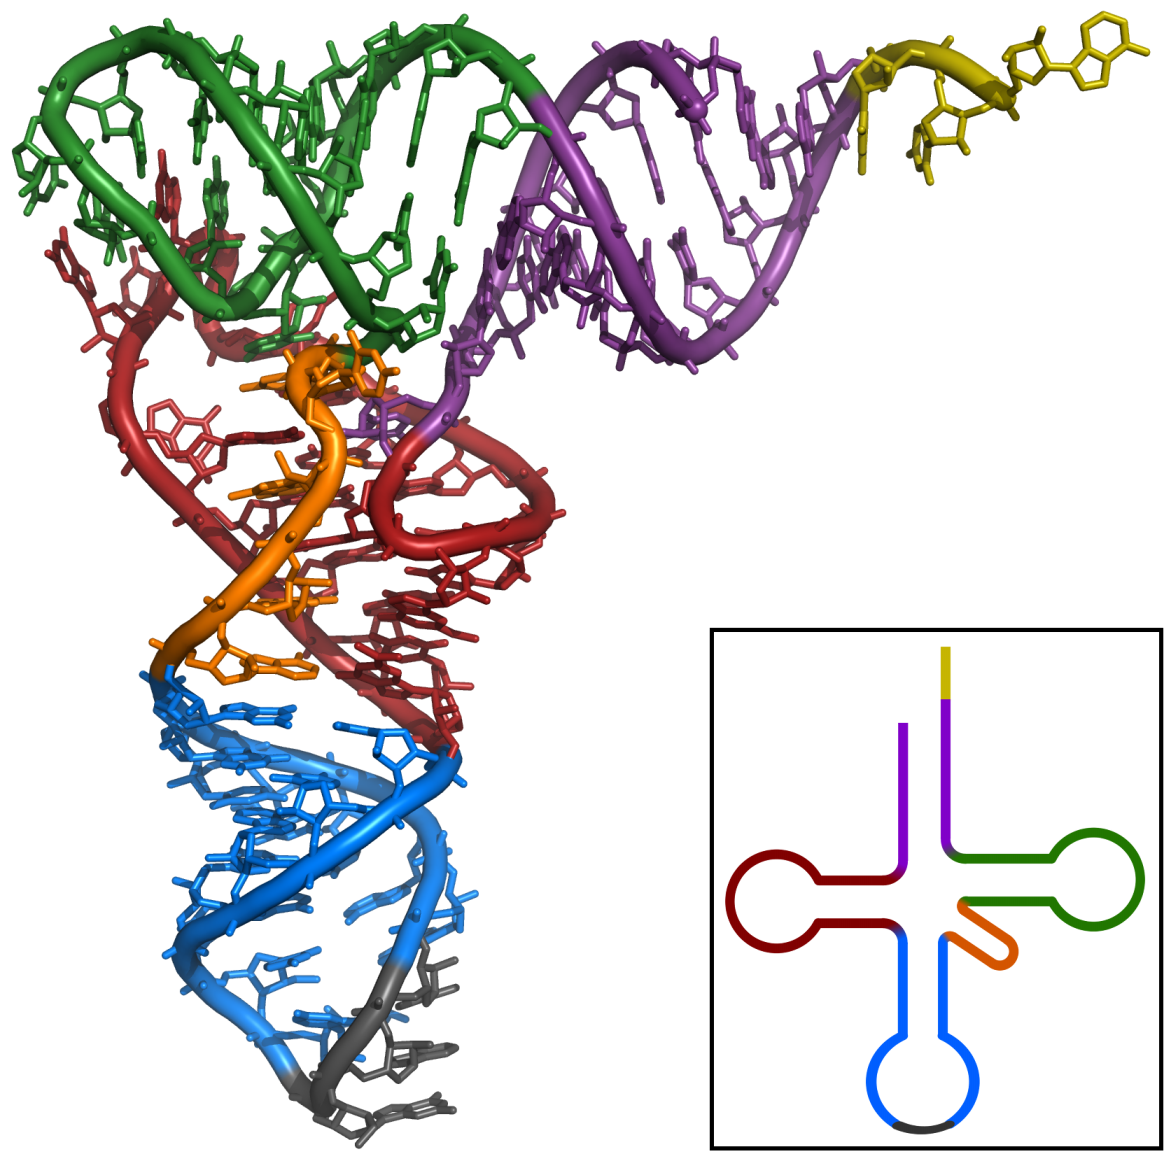
\includegraphics[width=\textwidth]{figures/chap3/TRNA-Phe_yeast_1ehz.png}
         \caption{}
         \label{fig:tRNA_3d_struct}
     \end{subfigure}
     \hfill
     \begin{subfigure}[b]{0.3\textwidth}
         \centering
         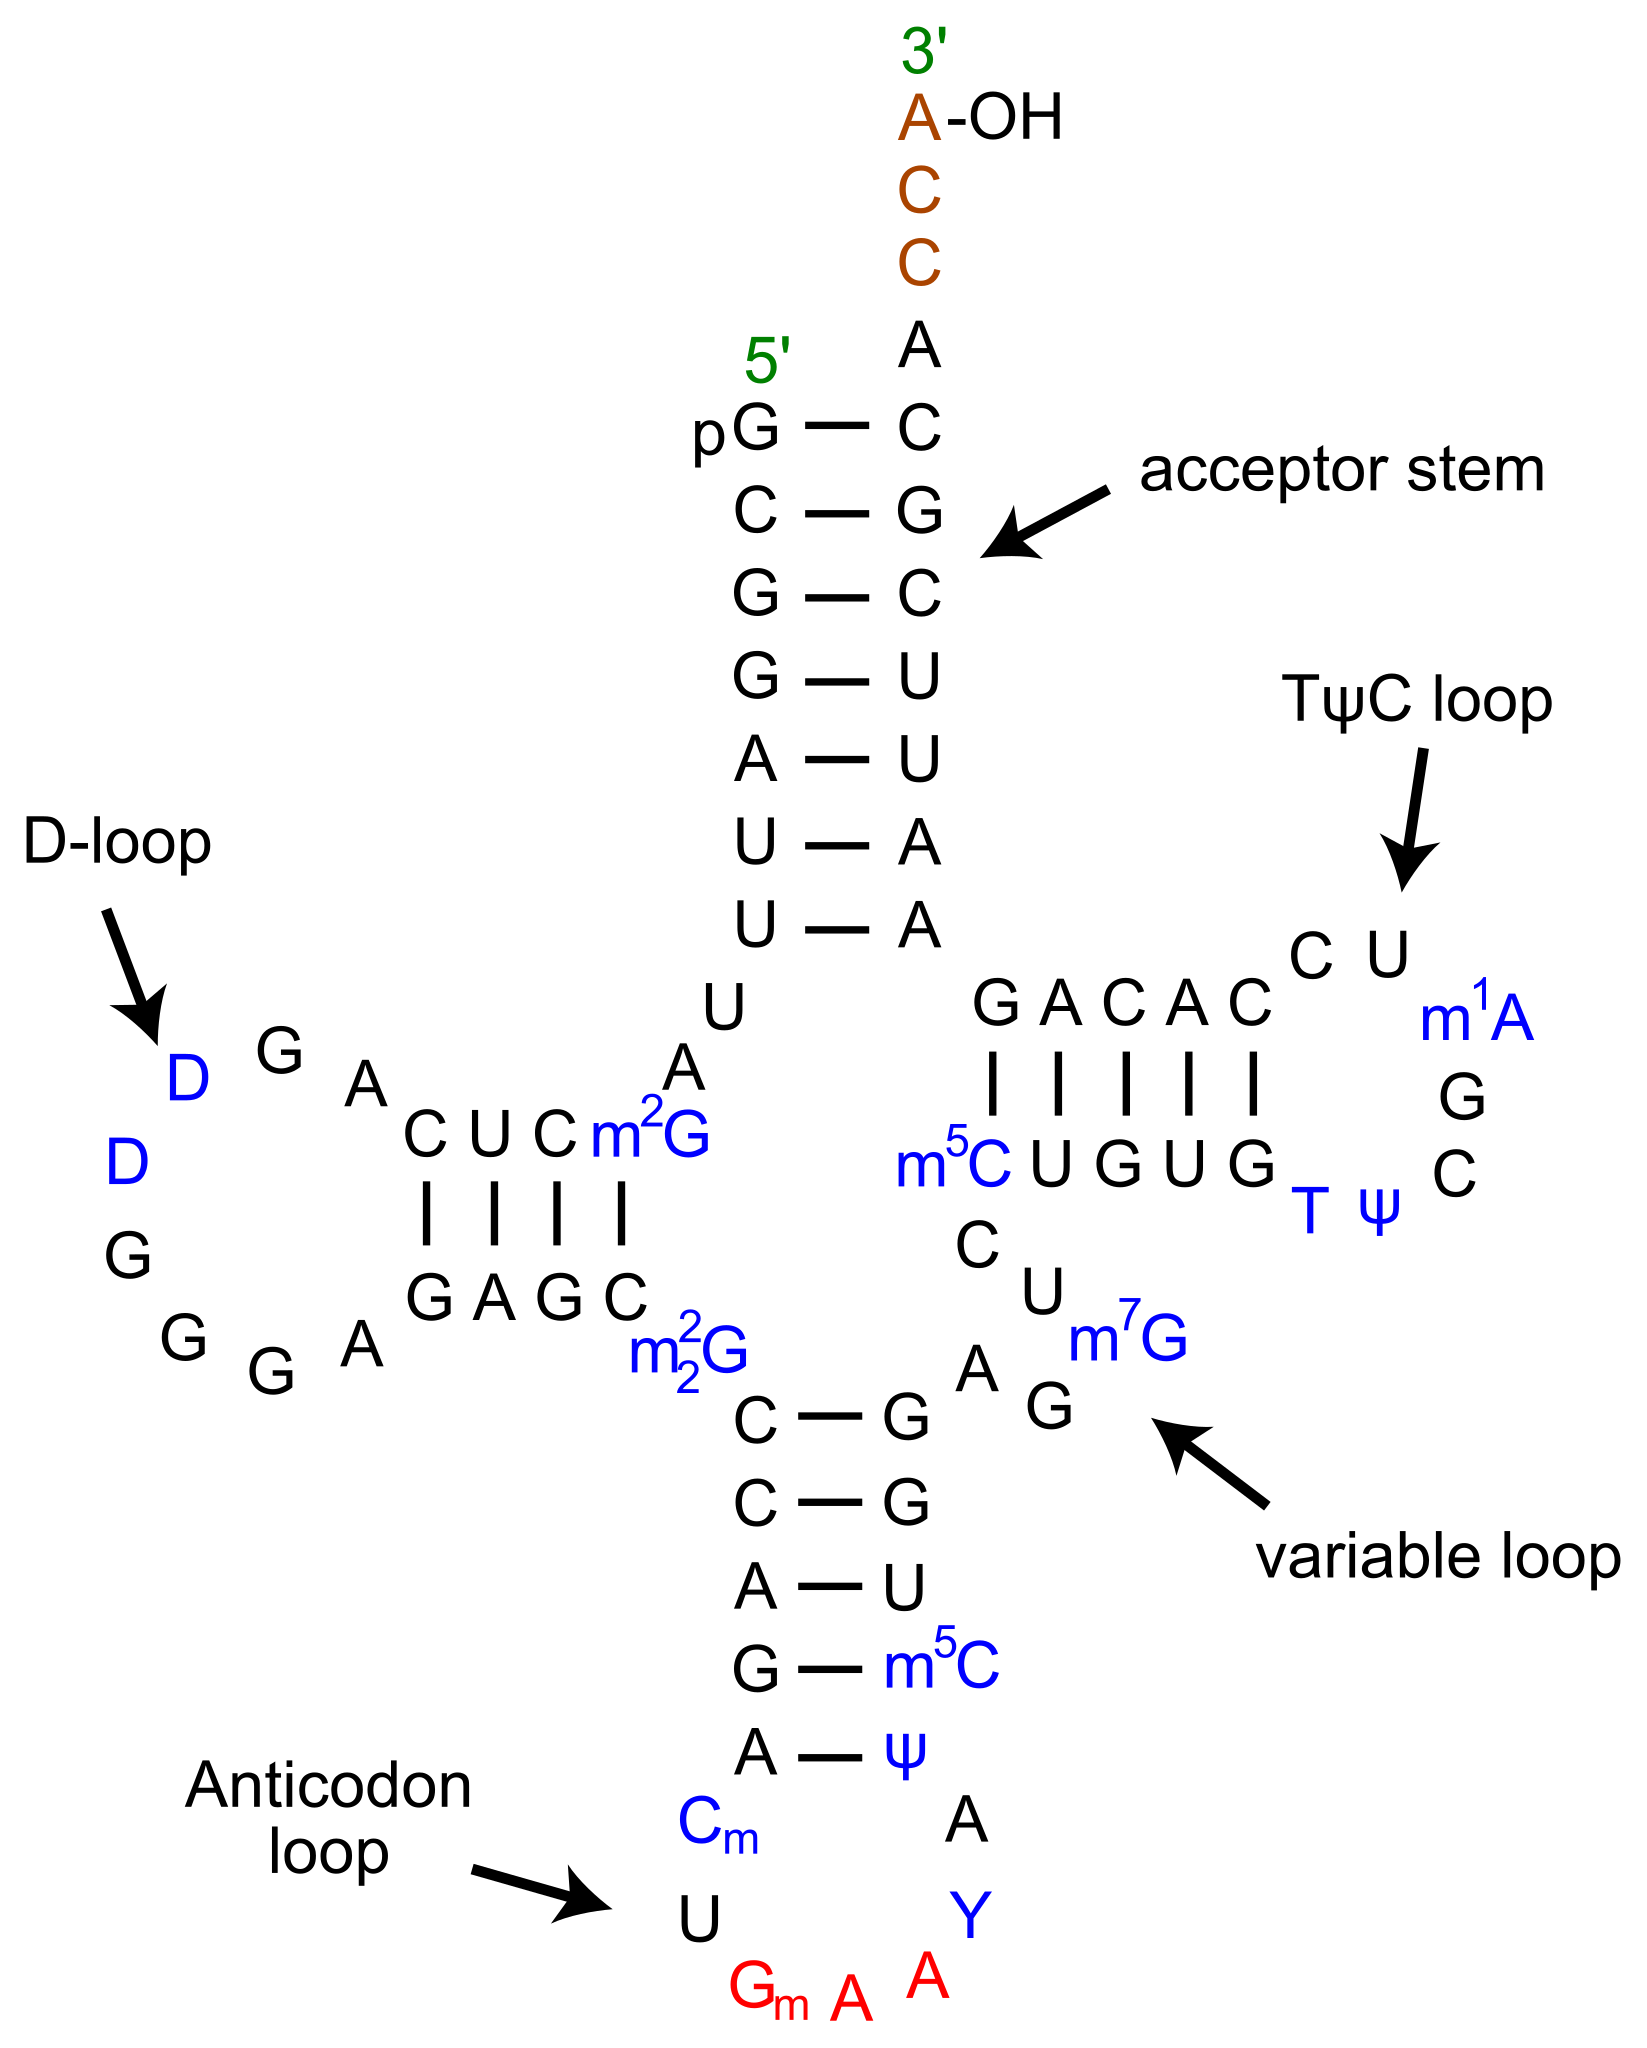
\includegraphics[width=\textwidth]{figures/chap3/TRNA-Phe_yeast_en.png}
         \caption{}
         \label{fig:tRNA_2d_struct}
     \end{subfigure}
     \hfill
     \begin{subfigure}[b]{0.2\textwidth}
         \centering
         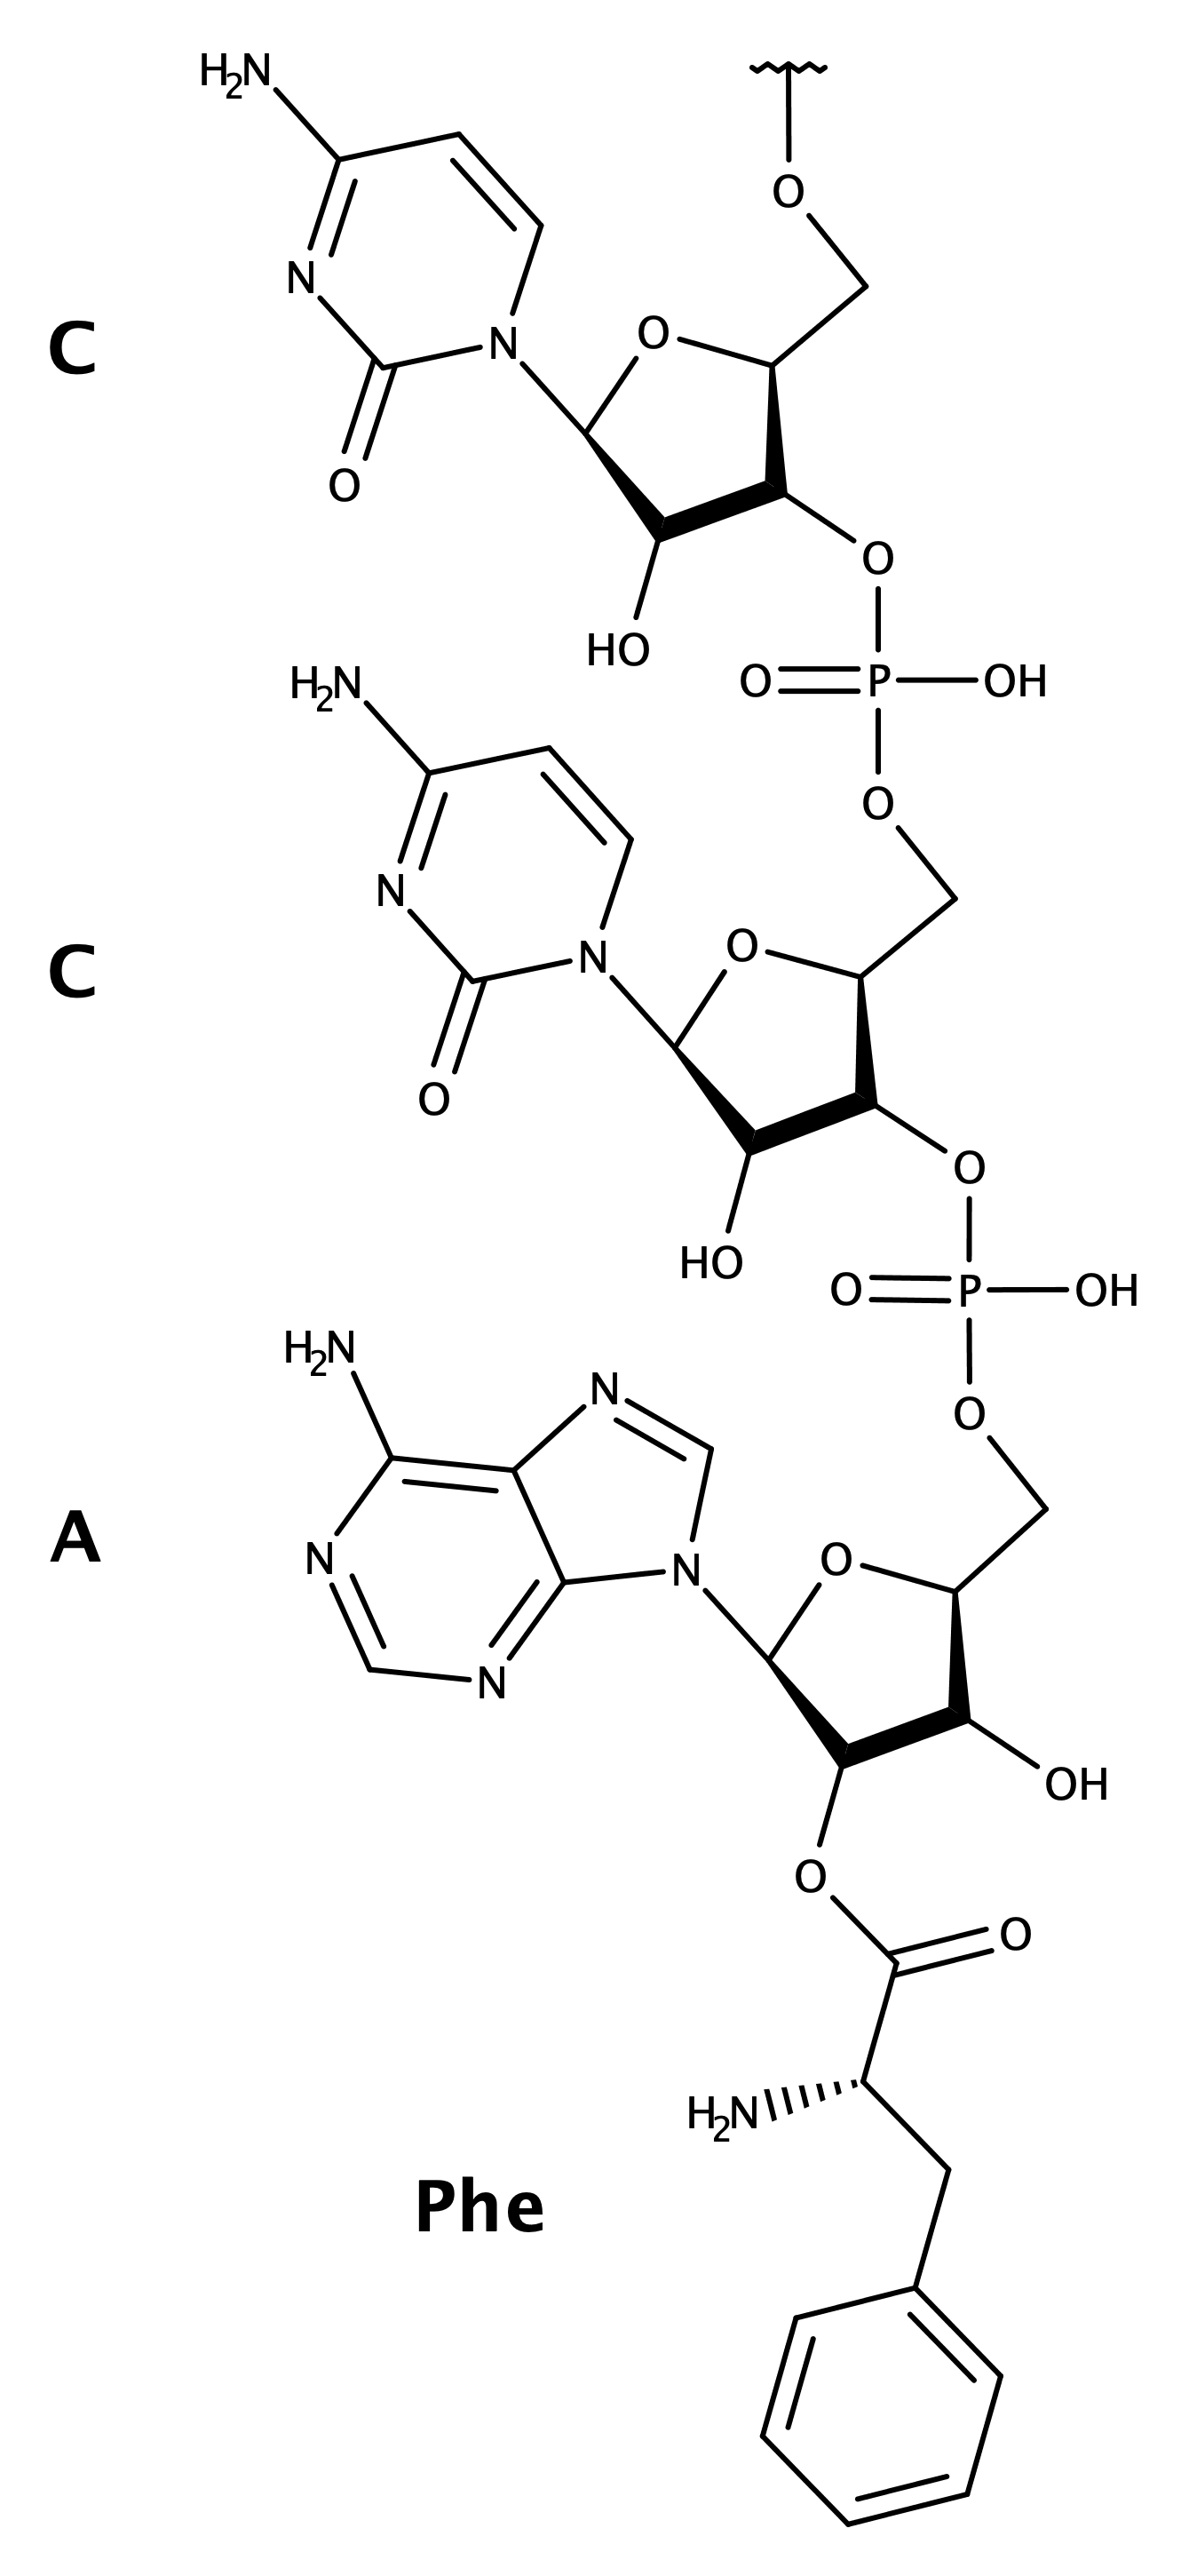
\includegraphics[width=\textwidth]{figures/chap3/CCA_Phe.png}
         \caption{}
         \label{fig:tRNA_CCAester}
     \end{subfigure}
        \caption{
        (a) Three dimensional structure of a tRNA colored by secondary structure elements shown in the insert, (b) secondary structure of a tRNA with names of the structural elements and some common base modifications, (c) the 3' CCA of a tRNA aminoacylated with phenylalanine.
        (a) and (b) from Yikrazuul, \href{https://creativecommons.org/licenses/by-sa/3.0}{CC BY-SA 3.0}, via Wikimedia Commons.
        }
\end{figure}





\begin{figure}
    \centering
    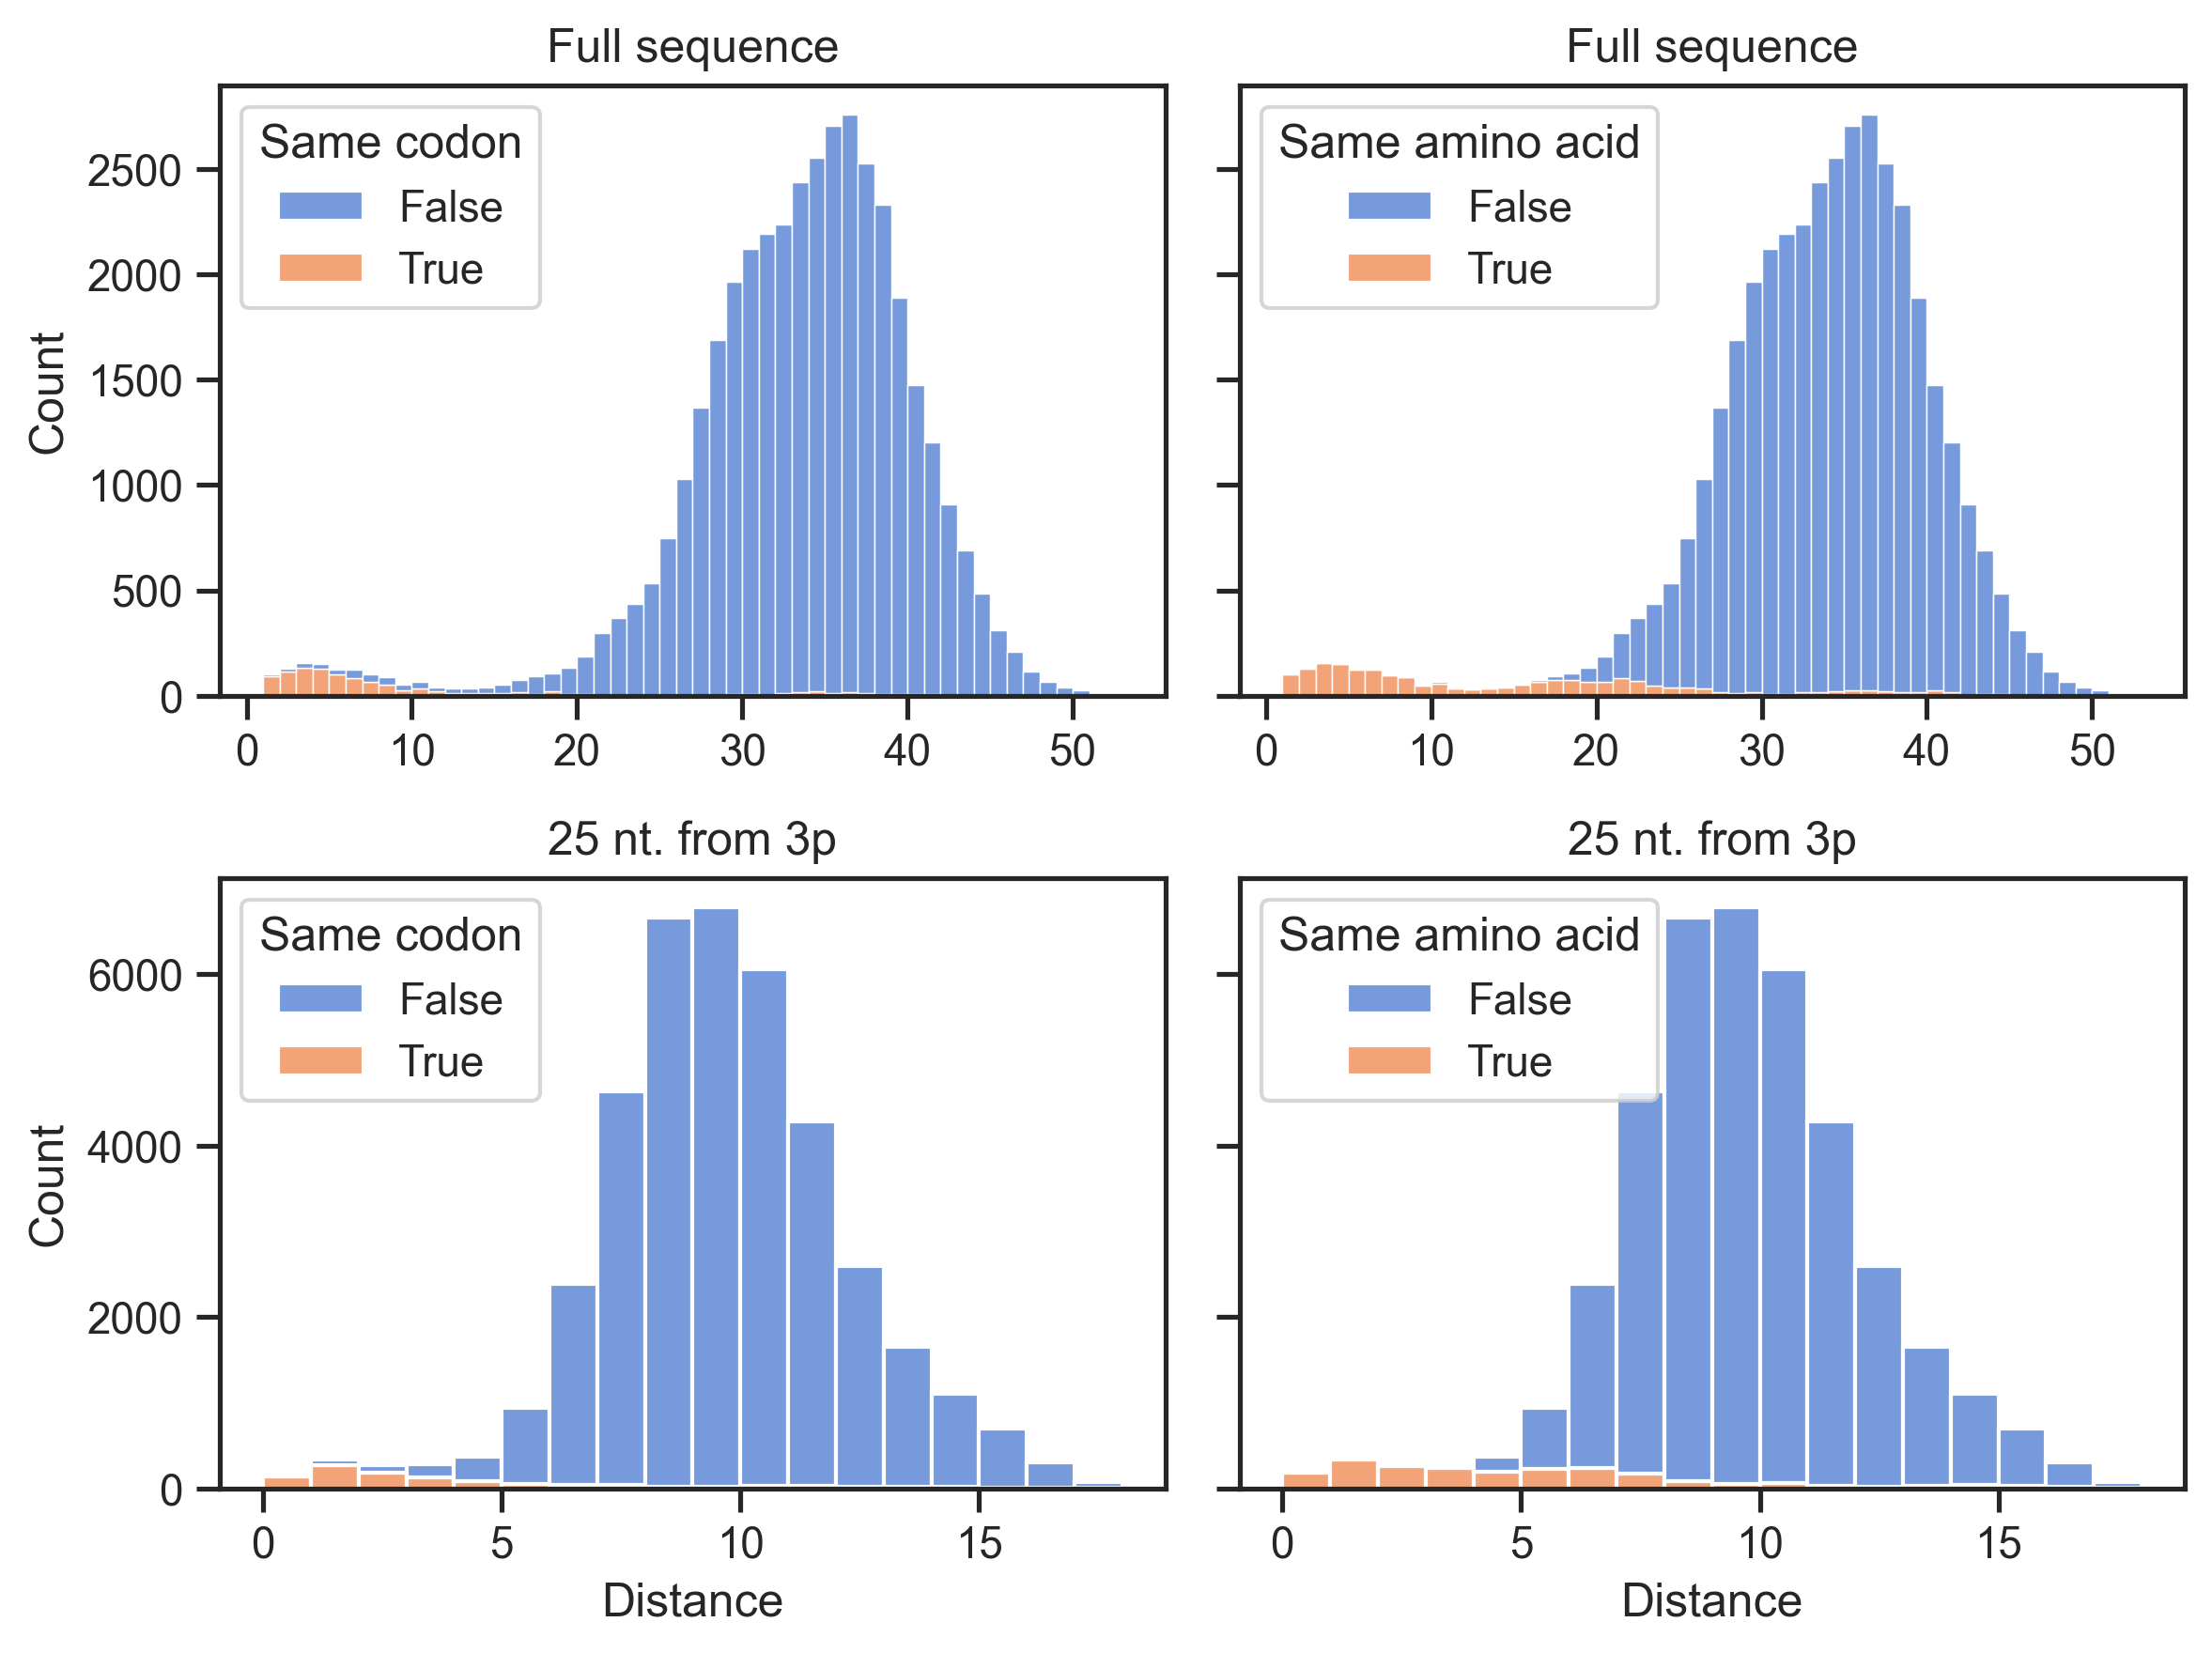
\includegraphics[width=\textwidth]{figures/chap3/tRNA_dist_hist.png}
    \caption{Histogram of the distances between tRNA transcripts after pairwise Needleman–Wunsch alignment. Distance is counted as the number of mismatches and gaps. The top row shows full sequence transcripts, the bottom row shows the last 25 nt. of each transcript. Distances are broken down by being between transcripts of the same codon or not, and same amino acid or not. Source: krdav Github \href{https://github.com/krdav/thesis_plotting/blob/main/tRNA_stats/plot_data.ipynb}{thesis\_plotting/tRNA\_stats}}
    \label{fig:dist_hist}
\end{figure}




\begin{table}[!htb]
\begin{tabular}{|l|p{0.85\textwidth}|}
\hline
Length & tRNAs \\ \hline
62     & m-Ser-AGC \\ \hline
68     & m-Arg-CGA \\ \hline
69     & m-Cys-UGC, m-Thr-ACA, m-Tyr-UAC \\ \hline
71     & m-Met-AUG, m-Trp-UGA, m-Pro-CCA, m-Gly-GGA, m-Asp-GAC \\ \hline
72     & m-Ser-UCA, m-Val-GUA, m-His-CAC, m-Ile-AUC, m-Glu-GAA, m-Ala-GCA \\ \hline
73     & c-Cys-UGC, m-Lys-AAA \\ \hline
74     & m-Phe-UUC, c-Gly-GGC, m-Leu-CUA, c-Ala-GCA, c-Gly-GGG \\ \hline
75     & c-Gln-CAG, c-Tyr-UAC, c-Ala-GCG, c-Ala-GCA, c-Gly-GGA, c-Pro-CCA,   c-Gln-CAA, c-Glu-GAG, c-Pro-CCU, c-Thr-ACA, c-Val-GUU, m-Gln-CAA, c-Asp-GAC,   c-Ala-GCU, c-Pro-CCG, c-Thr-ACG, c-His-CAC, c-Glu-GAA, c-Cys-UGC, c-Trp-UGG,   c-iMet-AUG \\ \hline
76     & c-Val-GUA, c-Arg-AGG, c-Tyr-UAU, c-Val-GUG, c-Ala-GCU, c-Tyr-UAC,   c-Arg-CGG, c-Met-AUG, m-Asn-AAC, c-Cys-UGC, c-Lys-AAG, c-Val-GUU, c-Arg-CGU,   c-Arg-CGA, c-Lys-AAA, c-Thr-ACA, c-Arg-AGA, c-Phe-UUC \\ \hline
77     & c-Thr-ACU, c-Ile-AUU, c-Ile-AUC, c-Lys-AAG, c-Asn-AAC, c-Leu-UUG,   c-Thr-ACA, c-Thr-ACG, c-Arg-AGA, c-Phe-UUC, c-Ile-AUA \\ \hline
78     & m-Leu-UUA, c-Asn-AAC \\ \hline
85     & c-Ser-UCG, c-Leu-CUU, c-Ser-AGC, c-Ser-UCU, c-Leu-CUA, c-Ser-UCA \\ \hline
86     & c-Leu-UUA, c-Leu-UUG, c-Leu-CUG \\ \hline
87     & c-Ser-AGC, c-Leu-UUG \\ \hline
90     & c-SeC-UGA \\ \hline
\end{tabular}
\caption{Mature human tRNA transcript lengths and the distribution among amino acids and codons. The tRNA column is populated with entries formatted as [cyto/mito]-[amino acid]-[codon] with [cyto/mito] indicated by c/m, [amino acid] indicated by the three letter amino acid code. Source: krdav Github \href{https://github.com/krdav/thesis_plotting/blob/main/tRNA_stats/plot_data.ipynb}{thesis\_plotting/tRNA\_stats}}
\end{table}
















\section{Quantifying aminoacylation}

Quantification of \textit{in vivo} transfer RNA (tRNA) aminoacylation is complicated by the many, highly similar, tRNA transcripts.
It was first with Northern blotting that tRNA transcripts could be resolved with sufficient resolution.
Aminoacylation can then be resolved by differential migration during electrophoresis and following probe quantification the level of aminoacylation, or charge, can be calculated \cite{Ho1987-ug, Varshney1991-zp, Stenum2017-wn}.





Multiple methods for quantifying aminoacylation these are...


\subsection{Northern blotting}
qwerty

\subsection{tRNA-seq}
Overview of the tRNA-seq methods.
Overview of the periodate-cleavage reaction.
Briefly, mention the array based tech introduced right before RNAseq.
Transition into giving an overview of each major advance in the methods.

\subsubsection{Zheng 2015}
Tao Pan RNAseq.
Extended by Evans 2017 to measure aminoacylation
\cite{Zheng2015-kj}


\subsubsection{Shigematsu 2017}
YAMAT seq


\subsubsection{Behrens 2021}
ghjm

\subsubsection{Others}
Here described other minor methodological advances/differences.
E.g. Wang [specifically amplified by GGT-ending primer during]







\subsection{The Malaprade-elimination reaction}
Dig deep into this reaction, the previous use, the chemistry etc.
This facilitates the discrimination between aminoacylated and unaminoacylated tRNA.
First used in Evans 2017, heavily inspired by the previous array based paper from Tao Pan's group.


\subsection{A lack of quantification rigor}
qwerty




\section{Strategy to improve tRNA-seq based aminoacylation quantification}


\section{Data processing}

\subsection{The alignment problem}
Blob on alignment:

* Maybe turn this into a wider discussion of annotation strategies and why it might be optimal to use masked sequences because this applies the least number of assumptions. A positional gap penalty would also help in that regard. HMM would be very strong but also would also make some assumptions about the modified sites that could be problematic in different contexts e.g. the HMM is fitted on data with a particular position always is modified but then in a biological context this modification is lost.
* Advantages: formalized model that calculated probabilities, can model site interactions, can model gaps and RT stops.
Modeling RT stops could be problematic though since it could easily vary depending on RT conditions, polymerases etc.
* Disadvantage: very slow, probably has to be refitted for new datasets because of slightly different RT conditions, also has to be refitted to take into account any biological changes in modification penetrance
* Pick a subset of reads with long alignments where the top scoring reference is several score points away from the runner up.
* Use these sequences to make an HMM for each annotation
* Run the HMMs on all sequences and calculate the annotation probability without the RT fall-off.
* Select all the sequences with an annotation with high HMM probability * away from the second best annotation.
* Refit the HMMs on these sequences.
* Run the HMMs on all sequences and calculate the annotation probability, this time with the RT fall-off included.
* Select sequences and refit HMM.
* Perform enough iterations to converge.





\section{Results}


\section{Methods}

\section{Discussion}




    \chapter{First degree dependence of aspartate for cell proliferation}

Closing chapter, dumping all the shitty unpublished data here.

\section{Introduction}
More blaa
 
    % bibliography
    %
    \bibliographystyle{plain}
    \bibliography{thesis}
 
    % appendices
    %
    \appendix
    \include{appxa}
    \include{appxb}
 
    \include{vita} 
    \end{document}
  \end{verbatim}
 \end{fullpage}
\end{figure}
 
The first section, from the \verb"\documentclass" to
the \verb"\begin\{document\}", defines the document class and options.
This thesis has specified two-sided formatting, which is now
allowed by the Graduate School.  Two sided printing is now
actually \LaTeX's default.  If you want one sided printing
you must specify \verb"oneside".
This sample also specified a font size
of 11 points. 
Possible font size options are: \verb"10pt", \verb"11pt", and \verb"12pt".
Default is 12 points, which is the preference
of the Graduate School. If you choose a smaller size be sure to
check with the Graduate School for acceptability.  The smaller fonts
can produce very small sub and superscripts.

Include most additional formatting packages with \verb"\usepackage",
as describe by Lamport\cite{Lbook}.  The one exception to this
rule is the \verb"natbib" package.  Include it with the \verb"natbib"
document option.
 
Use the \verb"\includeonly" command to format only a part of your
thesis.  See Lamport\cite[sec. 4.4]{Lbook} for usage and limitations.

 
\section{The Text Pages}
 
A chapter is a major division of the thesis.  Each chapter begins
on a new page and has a Table of Contents entry.
 
\subsection{Chapters, Sections, Subsections, and Appendices}
 
 
Within the chapter title use a \verb"\\" control sequence to separate lines
in the printed title (recall Figure \ref{start-2}.).
The \verb"\\" does not affect the Table of Contents entry.
 
Format appendices just like chapters.
The control sequence \verb"\appendix" instructs \LaTeX\ to
begin using the term `Appendix' rather than `Chapter'.
 
 
Sections and subsections of a chapter are specified
by  \verb"\section" and \verb"\subsection", respectively.
In this thesis chapter and section
titles are written to the table of contents.
Consult Lamport\cite[pg. 176]{Lbook} to see which
subdivisions of the thesis can be written to the table of contents.
The \verb"\\" control sequence is not permitted in section and
subsection titles.
 
 
\subsection{Footnotes}
 
\label{footnotes}
 Footnotes format as described in the \LaTeX\ book.  You can also
 ask for end-of-chapter or end-of-thesis notes.
 The thesis class will automatically set these up if
 you ask for the document class option \texttt{chapternotes}
 or \texttt{endnotes}.  
 
If selected, chapternotes will print automatically.  If you choose
endnotes however you must explicitly indicate when to print the notes 
with the command \verb"\printendnotes".  See the style guide for
suitable endnote placement.  

\subsection{Figures and Tables}
Standard \LaTeX\ figures and tables, see Lamport\cite[sec.~C.9]{Lbook},
normally provide the most convenient means to position the figure.
Full page floats and facing captions are exceptions to this rule.

If you want a figure or table to occupy a full page enclose the
contents in a \texttt{fullpage} environment.  
See figures~\ref{facing-caption}.

Facing page captions are described
in the Style Manual\cite{SP}.  They have different meanings
depending on whether you are using
the one-side or two-side thesis style.


If you are using the two-side style,
facing captions
are full page captions for full page figures or tables
and must face the illustration to which they refer.
You must explicitly format both pages. 
The caption part must appear on an even page
(left side) and the figure or table must
come on the following odd page (right side).
Enclose the float contents for the caption 
in a \texttt{leftfullpage} environment,
and enclose the float contents for the figure or table 
in a \texttt{fullpage} environment.
Figure~\ref{control-file}, for example,
required a full page so its caption (on a facing caption page)
would have been formatted as shown in figure~\ref{facing-caption}a.
The first page (left side) contains the caption. The second page
(right side) could be left blank.  A picture or graph might be pasted onto
this space.


\begin{figure}[t]
\footnotesize
\begin{verbatim}
     \begin{figure}[p]% the left side caption
       \begin{leftfullpage}
         \caption{ . . . }
       \end{leftfullpage}
     \end{figure}
     \begin{figure}[p]% the right side space
       \begin{fullpage}
          . . .
          ( note.. no caption here )
       \end{fullpage}
     \end{figure}
\end{verbatim}
\caption(a){This text would create a
  double page figure in the two-side style.}
\label{facing-caption}
\end{figure}
 
\begin{figure}[t]
\footnotesize
\begin{verbatim}
     \begin{figure}[p]
        \begin{leftfullpage}
           \caption{ . . . }
        \end{leftfullpage}
     \end{figure}
     \begin{figure}[p]% the right side space
       \begin{xtrafullpage}
          . . .
          ( note.. no caption here )
       \end{xtrafullpage}
     \end{figure}
\end{verbatim}
\caption(b)[Generating a facing caption page]{This text would create a
  facing caption page with the accompaning figure in the one-side style.}
\end{figure}
 
If instead you are using the one-side style,
facing caption pages are still
captions for full page figures or tables
that appear on the left-hand page (facing the illustration on the
right-hand page).  
However, the page number and binding offset are reversed
from their normal positions.
Format these captions by enclosing the float contents
in a \texttt{leftfullpage} environment.
Because you are printing on only one side of each sheet, you must manually
turn over this caption sheet. 
You then have the choice of inserting a preprinted illustration or
formatting one to print with the thesis. 
In either case no page number should appear
on the illustration page, nor should the page number increment. 
Enclose your figure's text
in an \texttt{xtrafullpage} environment, which will cause the
page numbers to come out right.  
You can, of course, leave out the illustration and insert a preprinted
copy later. 
Figure~\ref{facing-caption}b shows how to format a facing caption page
in the one-side style. Note that, in this case, the illustration
was also printed.

In the two-side style the \texttt{xtrafullpage} environment acts just like the
\texttt{fullpage} environment.  It does not produce a numberless page.


 
\subsection{Horizontal Figures and Tables}
Figures and tables may be formatted horizontally
(a.k.a.\ landscape) as long as their captions appear
horizontal also.  \LaTeX\ will format landscape material for you
if a couple of conditions are met.  You have to have a printer
and printer driver that allow rotations and
you have to have a couple of add-on \LaTeX\ packages.  

% Users of PostScript printers and Uniform Access computers 
% at the University of Washington will conform to both requirements,
% as will users of PC\TeX\ if they use postscript.

Include the \texttt{rotating} package 
\begin{demo}
\\usepackage[figuresright]\{rotating\}
\end{demo}
and read the documentation that comes with the package. 

Figure~\ref{sideways} is an example of how a landscape
table might be formatted. 

\begin{figure}[t]
\footnotesize
\begin{verbatim}
     \begin{sidewaystable}
         ...
         \caption{ . . . }
     \end{sidewaystable}
\end{verbatim}
\caption[Generating a landscape table]{This text would create a
  landscape table with caption.}
\label{sideways}
\end{figure}
 


\subsection{Figure and Table Captions}
Most captions are formatted with the \verb"\caption" macro as described 
by Lamport\cite[sec. C.9]{Lbook}. 
The uwthesis class extends this macro to allow
continued figures and tables, and to provide multiple figures and
tables with the same number, e.g., 3.1a, 3.1b, etc.
 
To format the caption for the first part of
a figure or table that cannot fit
onto a single page use the standard form:
\begin{demo}
\\caption[\textit{toc}]\{\textit{text}\}
\end{demo}
To format the caption for the subsequent parts of 
the figure or table 
use this caption:
\begin{demo}
\\caption(-)\{(continued)\}
\end{demo}
It will keep the same number and the text of the caption will be 
{\em(continued)}.

To format the caption for the first part of
a multi-part figure or table
use the format:
\begin{demo}
\\caption(a)[\textit{toc}]\{\textit{text}\}
\end{demo}
The figure or table will be lettered (with `a') as well as numbered.
To format the caption for the subsequent parts of 
the multi-part figure or table
use the format:
\begin{demo}
\\caption(\textit{x})\{\textit{text}\}
\end{demo}
where {\em x} is {\tt b}, {\tt c}, \ldots.
The parts will be lettered (with `b', `c', \ldots).

\section{The Preliminary Pages}
 
These are easy to format only because they are relatively invariant
among theses.  Therefore the difficulties have already been encountered
and overcome by \LaTeX\ and the thesis document classes.

Start with the definitions that describe your thesis.
This sample thesis was printed with the parameters:

\begin{demo}
\\Title\{The Suitability of the \\LaTeX\\ Text Formatter\\\\
   for Thesis Preparation by Technical and\\\\
   Non-technical Degree Candidates\}
\\Author\{Jim Fox\}
\\Program\{UW Information Technology\}
\\Year\{2012\}

\\Chair\{Name of Chairperson\}\{title\}\{Chair's department\}
\\Signature\{First committee member\}
\\Signature\{Next committee member\}
\\Signature\{etc\}

\end{demo}
 
Use two or more \verb"\Chair" lines if you have co-chairs.
 
\subsection{Copyright page}
Print the copyright page with \verb"\copyrightpage".

\subsection{Title page}
Print the title page with \verb"\titlepage".
The title page of this thesis was printed with%
\footnote{Actually, it wasn't.  I added a footnote---something you would not do.}
 
\begin{demo}
\\titlepage
\end{demo}
 
You may change default text on the title page with these
macros.  You will have to redefine \verb"\Degreetext", for instance,
if you're writing a Master's thesis instead of a dissertation.\footnote{If you use these they can
be included with the other information before \\copyrightpage".}

\begin{list}{}{\itemindent\parindent\itemsep0pt
   \def\makelabel#1{\texttt{\char`\\#1}\hfill}}
\item[Degree\char`\{{\it degree name}\char`\}]
   defaults to ``Doctor of Philosophy''
\item[School\char`\{{\it school name}\char`\}] defaults to
``University of Washington''
\item[Degreetext\char`\{{\it degree text}\char`\}] defaults to
``A dissertation submitted \ldots''
\item[textofCommittee\char`\{{\it committee label}\char`\}] defaults to
``Reading Committee:''
\item[textofChair\char`\{{\it chair label}\char`\}] defaults to
``Chair of the Supervisory Committee:''
\end{list}

These definitions must appear \underline{before} the \verb"\titlepage" command.

 
\subsection{Abstract}
Print the
abstract with \verb"\abstract".
It has one argument, which is the text of the abstract.
All the names have already been defined.
The abstract of this thesis was printed with
 
\begin{demo}
\\abstract\{This sample . . . `real' dissertation.\}
\end{demo}
 
 
\subsection{Tables of contents}
Use the standard \LaTeX\ commands to format these items.
 
 
\subsection{Acknowledgments}
Use the \verb"\acknowledgments" macro to format the acknowledgments page.
It has one argument, which is the text of the acknowledgment.
The acknowledgments of this thesis was printed with
 
\begin{demo}
\\acknowledgments\{The author wishes . . . \{\\it il miglior fabbro\}.\\par\}\}
\end{demo}
 
 
\subsection{Dedication}
Use the \verb"\dedication" macro to format the dedication page.
It has one argument, which is the text of the dedication.
 
\subsection{Vita}
Use the \verb"\vita" macro to format the curriculum vitae.
It has one argument, which chronicles your life's accomplishments.

Note that the Vita is not really a preliminary page.
It appears at the end of your thesis, just after the appendices.
 
 
%%  
%% \section{Customization of the Macros}
%%  
%% Simple customization, including 
%% alteration of default parameters,  changes to dimensions,
%% paragraph indentation, and margins, are not too difficult.
%% You have the choice of modifying the class file ({\tt uwthesis.cls})
%% or loading
%% one or more personal style files to customize your thesis.
%% The latter is usually most convenient, since you do not need
%% to edit the large and complicated class file.
%% 
 


% ========== Chapter 4
 
\chapter{Running \LaTeX\\
  ({\it and printing if you must})}
 
 
\TeX\ has been designed to produce exactly the same document
on all computers and on all printers.  {\it Exactly the same}
means that the various spacings, line and page breaks, and
even hyphenations will occur at the same places
when the document is formatted on a variety of computers.
However, the way you edit text files and run \LaTeX\ varies
from system to system.
 
\section{Running}

Unfortunately, the author is woefully out of water where 
\TeX\ on Windows is concerned.  Google would be his resource.
On a UNIX system he types

\begin{demo}
\$\ pdflatex uwthesis
\end{demo}

and it generally works.

 
\section{Printing}
 
All implementations of \TeX\ provide the option of {\bf pdf} output,
which is all the Graduate School now requires.  Even if you intend to
print a copy or two of your thesis---the best way to admire it---create a 
{\tt pdf} anyway.  It will print anywhere.

\printendnotes

%
% ==========   Bibliography
%
% \nocite{*}   % include everything in the uwthesis.bib file
\bibliographystyle{plain}
\bibliography{uwthesis}
%
% ==========   Appendices
%
\appendix
\raggedbottom\sloppy
 
% ========== Appendix A
 
\chapter{Where to find the files}
 
The uwthesis class file, {\tt uwthesis.cls}, contains the parameter settings,
macro definitions, and other \TeX nical commands which
allow \LaTeX\ to format a thesis.  
The source to
the document you are reading, {\tt uwthesis.tex},
contains many formatting examples
which you may find useful.
The bibliography database, {\tt uwthesis.bib}, contains instructions
to BibTeX to create and format the bibliography.
You can find the latest of these files on:

\begin{itemize}
\item My page.
\begin{description}
\item[] \verb%http://staff.washington.edu/fox/tex/uwthesis.html%
\end{description}

\item CTAN
\begin{description}
\item[]  \verb%http://tug.ctan.org/tex-archive/macros/latex/contrib/uwthesis/%
\item[]  (not always as up-to-date as my site)
\end{description}

\end{itemize}



\end{document}
